%%%%% Document class. %%%%
\documentclass [11 pt,	a4paper, notitlepage]{report}

%%%% Packages used. %%%%
% Math packages.
\usepackage{amsfonts}
\usepackage{amsmath} 
\usepackage{amssymb}
\usepackage{amsthm}
\usepackage{mathtools}
\usepackage{bbm}
\usepackage{mathrsfs}

% Language packages.
\usepackage[english, german]{babel}
\usepackage[ansinew]{inputenc}

% Other packages.
\usepackage{lipsum}
\usepackage{xcolor}
%\usepackage{showkeys}
\usepackage{float}
\usepackage{enumitem}

% Subfig, for figures.
\usepackage{subfig}


% FiXme package
\usepackage[draft, nofootnote, nomargin]{fixme}



%%% PGFPlot and TikZ. %%%%
\usepackage{tikz}
\usepackage{pgfplots}
\usetikzlibrary{positioning,intersections,calc, fit}

% Definition of node styles.
\tikzset{
	plain/.style={draw,circle, fill=white, minimum size = 1.6em, inner sep = 0.5},
	explored/.style = {circle, fill=gray, draw=black, very thick},
	discovered/.style = {circle, draw=black},
	neutral/.style = {circle, draw=black, minimum width=0.8em, inner sep=0},
	neutrallegend/.style = {circle, draw=black, minimum width=0.5em, inner sep=0}
}



%%%% BibLaTeX %%%%
% Set citestyle
%\usepackage[citestyle=authoryear]{biblatex}



%%%% Cosmetics. %%%%
% Set the style of chapter-headers: No "Chapter", only the number.
\usepackage{titlesec}
\titleformat{\chapter}
{\normalfont\LARGE\bfseries}{\thechapter}{1em}{}
\titlespacing*{\chapter}{0pt}{3.5ex plus 1ex minus .2ex}{2.3ex plus .2ex}



%%%% Theorems, Lemmas etc. %%%%
% All Theorems numbered by chapter.
% Theorem.
\newtheorem{theorem}{Theorem}[chapter]
% Lemma.
\newtheorem{lemma}[theorem]{Lemma}

% In Definition-style, i.e. no italics.
\theoremstyle{definition}
% Definition.
\newtheorem{definition}[theorem]{Definition}
% Note, not numbered.
\newtheorem*{note}{Note}

% Proofpart, to partition proofs
\newtheorem{proofpart}{Part}


% COMMANDS %%%%

%%%%%%%%%%%%%%%%%%%%%%%%%%%%%%%%%%%%%%%%%%%%%%%%%%%%%%%%%%%%
% General
%%%%%%%%%%%%%%%%%%%%%%%%%%%%%%%%%%%%%%%%%%%%%%%%%%%%%%%%%%%%

% Probability parameter (t or theta or...)
\newcommand{\pp}
	{\theta}

% BigO notation
\newcommand{\BigO}[1]
	{O\left(#1\right)}
\newcommand{\Smallo}[1]
	{o\left(#1\right)}
\newcommand{\OrderO}[1]
	{\Theta \left(#1\right)}
	
% Event E_{x}
\newcommand{\Event}[1]
	{\mathcal{E}_{#1}}
	
% càdlàq
\newcommand{\cadlag}
	{c\`{a}dl\`{a}g}	
	
% p(n)
\newcommand{\p}
	{p_n}
	
% Brownian motion
\newcommand{\Wt}
	{W^{\pp}}
\newcommand{\Bt}
	{B^{\pp}}
	
% l^2 space plus
\newcommand{\lp}
	{\mathit{l}^2_{+}}
% l^2 space down
\newcommand{\ld}
	{\mathit{l}^2_{\searrow}}	
	
% n{1,3} -> n^{1/3}]
\newcommand{\n}[2]
	{n^{#1 / #2}}
	
% \ps = \p/(1-(s-s)\p)
\newcommand{\ps}
	{\frac{\p}{1-(s-\floor{s})\p}}
% \psx{x} = x\p/(1-(s-s)\p)
\newcommand{\psx}[1]
	{\frac{#1 \p}{1-(s-\floor{s})\p}}
	
% Uniform rv Uij
\newcommand{\Uij}
	{U_{i,j}}
	
	
% \supns sup_{s<=n^2/3s0}
\newcommand{\supns}
	{\sup_{s \leq \n{2}{3} s_0 } }
	
% Condition in Expected Value, adds line and spaces.
\newcommand{\cond}
	{\: | \:}
% Expected value, regular brackets
\newcommand{\Exp}[1]
	{\mathbb{E}[#1]}
% Expected value, big fitted brackets
\newcommand{\ExpBig}[1]
	{\mathbb{E} \left[ #1 \right]}
% Ceiling
\DeclarePairedDelimiter\ceil{\lceil}{\rceil}
% Floor
\DeclarePairedDelimiter\floor{\lfloor}{\rfloor}

% Supremum-Norm 
\DeclarePairedDelimiter\norm{||}{||}
	
% Real numbers
\newcommand{\Real}
	{\mathbb{R}}
% Positive real numbers
\newcommand{\Rplus}
	{\mathbb{R}_+}
% Natural numbers
\newcommand{\Nat}
	{\mathbb{N}}
% Rational numbers
\newcommand{\Rat}
	{\mathbb{Q}}
	
% Space D[0, \infty]
\newcommand{\DInf}
	{D[0, \infty]}
% Space D[0, T]
\newcommand{\DT}
	{D[0, T]}
% Space C[0, \infty]
\newcommand{\CInf}
	{C[0, \infty]}
% Space C[0, T]
\newcommand{\CT}
	{C[0, T]}
	
% Borel 
\newcommand{\Bo}
	{\mathscr{B}}
% Borel sigma algebra
\newcommand{\Bosi}
	{Borel $\sigma$-algebra} 
	
% argmin
\DeclareMathOperator*{\argmin}
	{arg\,min}
	
% Binomial distribution
\DeclareMathOperator*{\Binom}
	{Bin}
% Bernoulli distribution
\DeclareMathOperator*{\Bern}
	{B}
% Exponential distribution
\DeclareMathOperator*{\Exponential}
	{Exp}
% Poisson distribution
\DeclareMathOperator*{\Poisson}
	{Poi}
		
% Indicator function
\newcommand{\Ind}[1]
	{\mathbbm{1}_{#1}}
	
% Interval [s, s+ds]
\newcommand{\sds}
	{[s, s+ds]}	
	
% Probability
\newcommand{\Prob}
	{\mathbb{P}}

% Sigma Algebra
\newcommand{\SigmaAlgebra}
	{\mathcal{F}}

% Probability space
\newcommand{\ProbSpace}
	{(\Omega, \SigmaAlgebra, \Prob)}


% Bounded function space
\newcommand{\Cb}
	{C_b}
% Compact function space
\newcommand{\CK}
	{C_K}
	
	
	
%%%%%%%%%%%%%%%%%%%%%%%%%%%%%%%%%%%%%%%%%%%%%%%%%%%%%%%%%%%%
% Graphs
%%%%%%%%%%%%%%%%%%%%%%%%%%%%%%%%%%%%%%%%%%%%%%%%%%%%%%%%%%%%
\newcommand{\Gnt}
	{\mathscr{G}(n, n^{-1} + \pp n^{-4/3})}
\newcommand{\Gcal}
	{\mathscr{G}}
\newcommand{\Ccal}
	{\mathcal{C}}
	
% Neighbour set
\newcommand{\Ni}[1]
	{\mathcal{N}_{#1}}
	
% Component C_i
\newcommand{\Ci}[1]
	{\mathcal{C}_{#1}}
% Component C^t_n 
\newcommand{\Cnt}
	{\mathcal{C}^{\pp}_n}
% Component C^t
\newcommand{\Ct}
	{\mathcal{C}^{\pp}}
% Component C^t_n bold
\newcommand{\Cntbold}
	{\boldsymbol{\mathcal{C}}^{\pp}_n}
% Component C^t bold
\newcommand{\Ctbold}
	{\boldsymbol{\mathcal{C}}^{\pp}}
	
% Number of ineligible vertices at time s.
\newcommand{\Ineligible}[1]
	{\eta_n(#1)}
	
% Event: New edge in interval I
\newcommand{\NewEdge}[1]
	{\Event{#1}}
	
	
%%%%%%%%%%%%%%%%%%%%%%%%%%%%%%%%%%%%%%%%%%%%%%%%%%%%%%%%%%%%	
% Processes 	
%%%%%%%%%%%%%%%%%%%%%%%%%%%%%%%%%%%%%%%%%%%%%%%%%%%%%%%%%%%%
% Zn -> Z_n()
\newcommand{\Zn}
	{Z_n}
% Znt -> Z_n^t()
\newcommand{\znt}
	{Z_n^{\pp}}
% Rescaled Z
\newcommand{\rznt}
	{\bar{Z}^{\pp}_n}
% Z - minZ process
\newcommand{\zminz}
	{B_n^{\pp}}
% Z - minZ process alt Prob Space
\newcommand{\zminzX}
	{\mathcal{B}_n^{\pp}}
% Rescaled Z-minZ process
\newcommand{\rzminz}
	{\bar{B}_n^{\pp}}

% An -> A_n()
\newcommand{\An}
	{F_n}
% Bn -> B_n()
\newcommand{\Bn}
	{G_n}
% Mn -> M_n()
\newcommand{\Mn}
	{M_n}
% Qn -> Q_n()
\newcommand{\Qn}
	{Q_n}
	
% Quadratic variation of Mn: [Mn]t
\newcommand{\Mnq}[1]
	{[M_n]_{#1}}
% an -> a_n()
\newcommand{\an}
	{a_n}
% amn -> a'_n() (a mark n)
\newcommand{\amn}
	{a'_n}
	
% Z, M, A, Q, B bar
\newcommand{\Zbar}
	{\bar{Z}_n}
\newcommand{\Abar}
	{\bar{F}_n}
\newcommand{\Mbar}
	{\bar{M}_n}
\newcommand{\Bbar}
	{\bar{G}_n}
\newcommand{\Qbar}
	{\bar{Q}_n}
	
% Ft filtration
\newcommand{\F}[1]
	{\mathcal{F}_{#1}}
% Ft filtration
\newcommand{\Fn}[1]
	{\mathcal{F}^n_{#1}}


% Surplus Edge Counting process N_n^t(.)
\newcommand{\nnt}
    {N_n^{\pp}}
% Surplus Edge Counting process N_n^t(.)
\newcommand{\nntX}
    {\mathcal{N}_n^{\pp}}
% Rescaled Surplus Edge Counting process N_n^t(.)
\newcommand{\rnnt}
    {\bar{N}_n^{\pp}}
% Limit N^t process 
\newcommand{\Nt}
	{N^{\pp}}    
% Limit N^t process alt prob space
\newcommand{\NtX}
	{\mathcal{N}^{\pp}}    
% N in discrete time (M_n?)
\newcommand{\Ndis}
	{\mathcal{M}_n^{\pp}}
% N in discrete time (M_n?)
\newcommand{\rNdis}
	{\bar{M}_n^{\pp}}
% N in discrete time (M_n?) alt prob space
\newcommand{\rNdisX}
	{\bar{\mathcal{M}}_n^{\pp}}
    
% Zeta = C^-1_n()
\newcommand{\ZetaMinus}[1]
	{\zeta^{-1}_n(#1)}
% Zeta = C^-1_n()
\newcommand{\Zetan}[1]
	{\zeta^{-1}_n(#1)}
	
% Alternate processes using Skorohod
% Rescaled Z
\newcommand{\rzntX}
	{\bar{\mathcal{Z}}^{\pp}_n}
% Brownian motion
\newcommand{\WtX}
	{\mathcal{W}^{\pp}}
% Reflected BM
\newcommand{\BtX}
	{\mathcal{B}^{\pp}}
% SE counting process
\newcommand{\rnntX}
	{\bar{\mathcal{N}}_n^{\pp}}
	
	
%%%%%%%%%%%%%%%%%%%%%%%%%%%%%%%%%%%%%%%%%%%%%%%%%%%%%%%%%%%%
% Rest (Chapter specific)
%%%%%%%%%%%%%%%%%%%%%%%%%%%%%%%%%%%%%%%%%%%%%%%%%%%%%%%%%%%%

% Deterministic lemma
\newcommand{\tn}[1]
	{t_{n, #1}}
\newcommand{\tip}
	{t_{i+1}}
\newcommand{\xip}
	{x_{i+1}}
\newcommand{\lnx}
	{l_n(x^*)}
\newcommand{\rnx}
	{r_n(x^*)}
\newcommand{\fnPoints}
	{\mathcal{T}_n}
	
% Lemma 8
\newcommand{\Xin}
	{\Xi^{(n)}}
\newcommand{\XinX}
	{\Xi^{\prime (n)}}
\newcommand{\XiX}
	{\Xi^{\prime}}
	
% [0, \infty) \times (0, \infty)
\newcommand{\IntTimesInt}
	{[0, \infty) \times (0, \infty)}
	
% E{\delta, c}
\newcommand{\ExcursionEvent}
	{\Event{\delta, C, n}}
	
% Chi_alpha^n
\newcommand{\ChiAn}
	{\chi^\alpha_n}
	
% Mean number of components in interval #1
\newcommand{\NComp}[1]
	{q(n,#1)}
	
%S Surplus sigma^t_n
\newcommand{\sigmant}
	{\mathcal{\sigma}^{\pp}_n}
%S Surplus sigma^t
\newcommand{\sigmat}
	{\mathcal{\sigma}^{\pp}}
%S Surplus sigma^t boldbold
\newcommand{\sigmatbold}
	{\boldsymbol{\mathcal{\sigma}}^{\pp}}
	

%%%%%%%%%%%%%%%%%%%%%%%%%%%%%%%%%%%%%%%%%%%%%%%%%%%%%%%%%%%%
% Outlook
%%%%%%%%%%%%%%%%%%%%%%%%%%%%%%%%%%%%%%%%%%%%%%%%%%%%%%%%%%%%
% Bold x vector
\newcommand{\x}
	{\boldsymbol{x}}
\newcommand{\xn}
	{\boldsymbol{x}^{(n)}}
\newcommand{\X}
	{\boldsymbol{X}}

% Probability parameter
\newcommand{\q}
	{q}
\newcommand{\qn}
	{q^{(n)}}
	
% Sigma^(n)
\newcommand{\sign}
	{\sigma^{(n)}}
	
% Random graph
\newcommand{\Wrg}
	{\mathscr{W}}

% BF-walk on W(x,q)
\newcommand{\bfw}
	{Z}
% BF-walk on W(xn, qn)
\newcommand{\bfwn}
	{Z_n}
% Rescaled BF-walk on W(x, q)
\newcommand{\rbfw}
	{\bar{Z}_n}
% Rescaled BF-walk on W(xn, qn)
\newcommand{\rbfwn}
	{\bar{Z}_n}

% x star n
\newcommand{\xsn}
	{x_*^{(n)}}

% Yn vector
\newcommand{\Yn}
	{{Y}^{(n)}_k}
% Y vector
\newcommand{\Y}
	{{Y}}
% Ynk vector
\newcommand{\Ynk}
	{{Y}^{(n)}_k}
% Yk vector
\newcommand{\Yk}
	{{Y}_k}
% gamma_n: Rescaled excursion of rznt
\newcommand{\rgamman}
	{\bar{\gamma}^{(n)}}
\newcommand{\rsigman}
	{\bar{\sigma}^{(n)}}

% YnX vector
\newcommand{\YnX}
{Y^{(n)}_k}
% Y vector
\newcommand{\YX}
{Y}
% Yn vector
\newcommand{\YnkX}
{Y^{(n)}_k}
% Y vector
\newcommand{\YkX}
{Y_k}


\usepackage[nopostdot, nonumberlist, toc, style = super]{glossaries}
\makenoidxglossaries 

% Numbers
\newglossaryentry{nat}
{
	name={$\Nat$},
	description={Natural numbers, excluding 0}
}
\newglossaryentry{nat0}
{
name={$\Nat_0$},
description={Natural numbers, including 0}
}
\newglossaryentry{rat}
{
name={$\Rat$},
description={Rational numbers}
}
\newglossaryentry{real}
{
	name={$\Real$},
	description={Real numbers}
}
\newglossaryentry{realpos}
{
name={$\Real_{\geq 0}$},
description={Positive real numbers}
}

% Graphs
\newglossaryentry{ergraphp}
{
name={$\mathscr{G}(n,p)$},
description={Erd\"os-Renyi random graph on $n$ vertices with edge-probability $p$}
}
\newglossaryentry{ergraphm}
{
	name={$\mathscr{G}(n,m)$},
	description={Erdös-Renyi random graph on $n$ vertices with $m$ edges}
}
\newglossaryentry{prob}
{
name={$\p$},
description={Edge-probability in $\Gnt$}
}

% Processes
\newglossaryentry{zsmall}
{
name={$z(i)$},
description={Breadth-first walk in discrete time}
}
\newglossaryentry{znt}
{
name={$\znt(s)$},
description={Breadth-first walk in continuous time}
}
\newglossaryentry{rznt}
{
name={$\rznt$},
description={Rescaled breadth-first random walk}
}
\newglossaryentry{bm}
{
name={$W$},
description={Standard Brownian motion}
}
\newglossaryentry{bmt}
{
name={$\Wt$},
description={Brownian motion with drift}
}
\newglossaryentry{bmtr}
{
name={$\Bt$},
description={Reflected Brownian motion with drift}
}

% Distributions
\newglossaryentry{Unif}
{
	name={$U[a,b]$},
	description={Uniform distribution on $[a,b]$}
}
\newglossaryentry{Binom}
{
name={$\Binom(n,p)$},
description={Binomial distribution with parameters $n$, $p$}
}
\newglossaryentry{Bern}
{
name={$\Bern(p)$},
description={Bernoulli distribution with parameter $p$}
}
\newglossaryentry{Exponential}
{
name={$\Exponential(\lambda)$},
description={Exponential distribution with parameter $\lambda$}
}
\newglossaryentry{Poisson}
{
name={$\Poisson(\lambda)$},
description={Poisson distribution with parameter $\lambda$}
}

% Rest
\newglossaryentry{Ind}
{
name={$\Ind{x}$},
description={Indicator function of $x$}
}
\newglossaryentry{SigmaAlgebra}
{
name={$\SigmaAlgebra$},
description={$\sigma$-algebra}
}
\newglossaryentry{SigmaAlgebrat}
{
name={$\SigmaAlgebra_t$},
description={Natural filtration generated by $(\znt(s), s \leq t)$}
}
\newglossaryentry{Event}
{
name={$\Event{X}$},
description={Event, defined by $X$}
}


\makeindex

\title{
	{Thesis Title}\\
	{Universit\"at Leipzig}
}
\author{David Biesner}
\date{\today}

\begin{document}
	
	\maketitle
	
	\newpage
	% Abstract
% Contains a short summary in English and German

\selectlanguage{english}
\begin{abstract}	
%	The Erdös-Renyi random graph $\Gcal(n, \p)$ on $n$ vertices with edge probability $\p = n^{-1} + \pp \n{-4}{3}$
%	for some $\pp \in \Real$ is called critical and its component sizes are of order $\n{2}{3}$.
	
	Based on a 1997 paper by David Aldous we analyse component sizes in the critical Erdös-Renyi random graph,
	$\Gcal(n, \p)$ with edge probability $\p = n^{-1} + \pp \n{-4}{3}$ for some $\pp \in \Real$.
	
	In general, component sizes will be of order $\n{2}{3}$.
	As $n \rightarrow\infty$, the ordered component sizes and corresponding counts of surplus edges
	(both rescaled by $\n{-2}{3}$) converge in distribution to a limit.
	
	Attach a downward drift $\pp - t$ to a Brownian motion $W(t)$ by $\Wt(t) = W(t) + \int_0^t(\pp-s)ds$
	and reflect this process at the $x$-axis by $\Bt(t) = \Wt(t) - \min_{s \leq t} \Wt(s)$.
	The limit of component sizes and surplus edges is distributed as the ordered lengths of excursions of $\Bt$ above zero 
	and marks of a Poisson point process with rate $\Bt$.
	
	While parts of the original paper rely on deep results on random graphs about bounds on the number of tree components, 
	unicyclic components and complex components, 
	we provide a self-contained proof that substantially simplifies the argument.
	
\end{abstract}

	% Dedication
% Probably in German

\chapter*{Danksagung}
	
	\tableofcontents 
	\newpage
	
	\cleardoublepage
	% \phantomsection
	\addcontentsline{toc}{chapter}{\listfigurename}
	\listoffigures
	
	\glsaddall
	\printnoidxglossary[title={List of Symbols}, sort=def]
	
	% Chapter 1: Introduction
% Contains:
%   An introduction to random graph theory
%   Basic results on the size of random graph components
%   Basic results on the critical window
%   The main theorem:
%      Motivation
%      The Brownian motion
%      Complete statement
%   Overview of coming proof

\chapter{Introduction}
\fxnote{Update title.}

The study of randomly generated graphs started in 1959,
when Paul Erd\H{o}s and Alfréd Rényis paper "On random graphs", \cite{Erdos.1959},
and Edgar Gilberts paper "Random graphs", \cite{Gilbert.1959},
introduced what is now known as the \emph{Erd\H{o}s-Rényi model} of random graphs.

Starting with the original papers,
the examination of sizes of connected components in such graphs was of great interest.
David Aldous 1997 paper "Brownian excursions, critical random graphs and the multiplicative coalescent", \cite{Aldous.1997},
which provides the basis for this thesis,
examines component sizes in the so-called critical Erd\H{o}s-Rényi random graph as the number of vertices $n$ grows to infinity.

This thesis will provide a strict proof of one of the the main results of this paper.
If no other reference is given, each result (or an equivalent thereof) can be found in Chapters 1 and 2 of \cite{Aldous.1997}.


\section{The Erd\H{o}s-Rényi random graph}
%%%%%%%%%%%%%%%%%%%%%%%%%%%%%%%%%%%%%%%%%%%%%%%%%%%%%%%%%%%%
% SECTION: The Erd\H{o}s-Rényi random graph
%%%%%%%%%%%%%%%%%%%%%%%%%%%%%%%%%%%%%%%%%%%%%%%%%%%%%%%%%%%%

In their paper, Erd\H{o}s and Rényi proposed a model of random graph that is now known as the Erd\H{o}s-Rényi random graph.
There are several ways to construct this random graph which we will briefly introduce,
starting with the historic models used in this first paper 
and continuing with the equivalent model which provides the basis for Aldous' paper and consequently this thesis.

We denote by $G_{n,M}$ the set of graphs on $n$ vertices with $M$ edges that are
\begin{enumerate}
	\item undirected,
	\item without slings, i.e. there is no edge $(v,v)$ for some vertex $v$,
	\item without parallel edges, i.e. there can be at most one edge $(v_1, v_2)$ for each pair of vertices.
\end{enumerate}
A graph in $G_{n,M}$ can be constructed by choosing $M$ out of the $\binom{n}{2}$ possible edges between the vertices,
which leads to a total number of graphs
\begin{equation}
	|G_{n,M}| = \binom{\binom{n}{2}}{M}.
\end{equation}
The Erd\H{o}s-Rényi random graph $\Gcal(n, M)$ is now obtained by choosing one element of $G_{n,M}$ at random
with equal probability for each graph, where the number of edges is usually dependent on the number of vertices, $M = M(n)$.

An equivalent definition provides the following process:
Starting with a graph on $n$ vertices with $0$ edges at time $t=1$, 
pick one of the $\binom{n}{2}$ possible edges at random with equal probability for each edge,
label it $e_1$.
At time $t=2$ pick one of the remaining $\binom{n}{2}-1$ edges, again all remaining edges being equiprobable,
and denote it by $e_2$.
Continue until $M$ edges have been chosen at time $t=M$.
The graph $(V,E)$ on vertices $V = \{1, \dots, n\}$ with edges $E = \{e_1, \dots, e_M\}$ is the desired Erd\H{o}s-Rényi random graph.

Using these definitions Erd\H{o}s and Rényi prove that,
when increasing the number of edges $M(n)$,
the sizes of connected components undergo distinct phases leading from small sparse components and unconnected vertices
to one giant component and eventually a completely connected graph.

Most current literature and the paper we are studying uses a slightly different approach to the construction of this random graph.
Given a set of vertices $\{1, \dots, n\}$ and an edge-probability $\p = p(n)$
we take every edge $(v_1, v_2)$ and add it to the set of edges $E$ of the random graph with probability $\p$ independently.
We call an edge $e = (v_1, v_2)$ open if $e \in E$, closed otherwise.
We denote a random object constructed this way by $\Gcal(n, \p)$\label{I: gnt} and expect a realisation of the random graph to have $\binom{n}{2}\p$ edges.
When increasing the probability $\p$ from $0$ to $1$ the resulting random graph undergoes the same so-called phase transitions
discovered by Erd\H{o}s and Rényi.

These phase transitions include a sudden dramatic increase in average component size happening around $M(n) = \frac{n}{2}$ or $\p = \frac{1}{n}$
which we study in this thesis.
The following section will provide a more precise introduction to the different phases a random graph undergoes
with increasing number of edges.


\section{General results on component sizes}
%%%%%%%%%%%%%%%%%%%%%%%%%%%%%%%%%%%%%%%%%%%%%%%%%%%%%%%%%%%%
% SECTION: General results on component sizes
%%%%%%%%%%%%%%%%%%%%%%%%%%%%%%%%%%%%%%%%%%%%%%%%%%%%%%%%%%%%

To provide an overview of the aforementioned phases
which the component sizes of the Erd\H{o}s-Rényi random graph pass through,
we discuss relevant results that were established previous to \cite{Aldous.1997}.

We begin with the subcritical graph, that is
$\Gcal(n, \p)$ with $\p < \frac{1}{n}$
or $\lambda = n \p < 1$.
The following theorem provides a lower bound on the size of $\Ccal_{\max}$, the largest component of $\Gcal$.
\begin{theorem}[Lower bound on largest subcritical component, {\cite[Theorem 4.4, p.125]{vanderHofstad.2016}}]
	Fix $\lambda < 1$. 
	Then, for all $a > 1/I_{\lambda}$, 
	there exists $\delta = \delta(a, \lambda)$ such that
	\begin{equation}
		\Prob( |\Ccal_{\max}| \geq a \log n ) = \BigO{n^{-\delta}},
	\end{equation}
	where 
	\begin{equation}
		I_{\lambda} = \lambda - 1 - \log(\lambda).
	\end{equation}
	is the large deviation rate function for Poisson random variables with mean $\lambda$.
\end{theorem}
The next theorem gives an upper bound for the size of $\Ccal_{\max}$.
\begin{theorem}[Upper bound on largest subcritical component, {\cite[Theorem 4.5, p.125]{vanderHofstad.2016}}]
	Fix $\lambda < 1$. 
	Then, for all $a < 1/I_{\lambda}$, 
	there exists $\delta = \delta(a, \lambda)$ such that
	\begin{equation}
	\Prob( |\Ccal_{\max}| \leq a \log n ) = \BigO{n^{-\delta}}.
	\end{equation}
\end{theorem}
Together, these theorems imply
\begin{equation}
	\frac{|\Ccal_{\max}|}{\log n} \rightarrow_p 1/I_{\lambda}.
\end{equation}
and therefore the expected largest component size will be of order $\log n$.

\bigskip

Consider the opposite case, the supercritical graph with $\lambda > 1$.
Denote by $\xi_\lambda$ the survival probability of a Poisson branching process with mean offspring $\lambda$.
Note that $\xi_\lambda > 0$ since $\lambda > 1$
(For an introduction into the theory of branching processes with application in random graphs, 
see \cite[Chapter 3, p.87ff.]{vanderHofstad.2016}).
Any vertex is part of a large component with probability $\xi_\lambda$, 
therefore we will expect around $n \xi_\lambda$ vertices being part of large connected components.
The following theorem now states that all of these vertices are, in fact, part of the same connected component, which we call the giant component.

\begin{theorem}[Law of large numbers for giant component, {\cite[Theorem 4.8, p.131]{vanderHofstad.2016}}]
	Fix $\lambda>1$.
	Then, for all $\nu \in (\frac{1}{2}, 1)$, there exists $\delta = \delta(\nu, \lambda)$ such that
	\begin{equation}
		\Prob\left( \left| |\Ccal_{\max}| - n \xi_\lambda \right| \geq n^{\nu}\right) = \BigO{n^{-\delta}}.
	\end{equation}
\end{theorem}

\begin{figure}[h]
	\centering
	\subfloat[$\lambda = 0.5$]{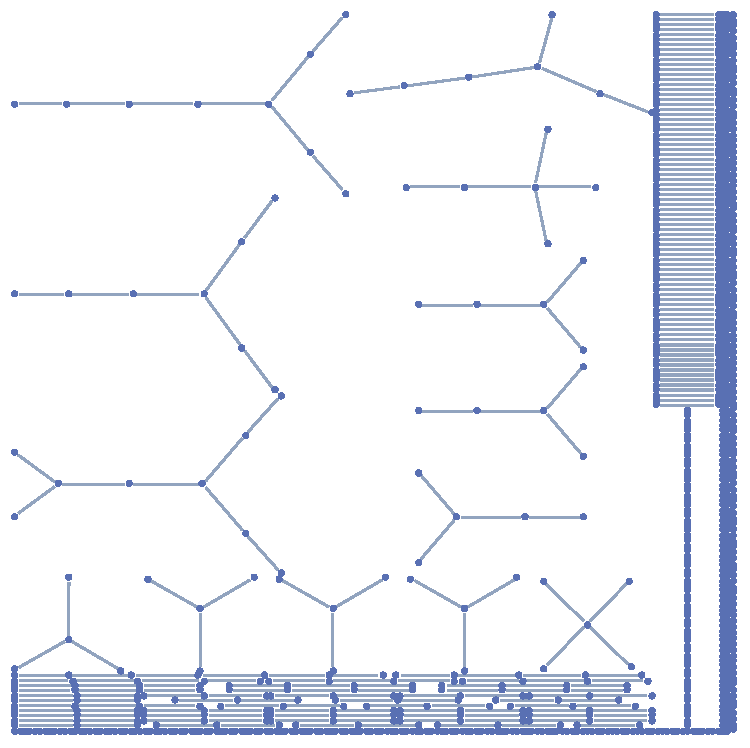
\includegraphics[page=1,width=.31\textwidth]{figures/chapter1/ER_1000_-5}}%
	\quad
	\subfloat[$\lambda = 1.5$]{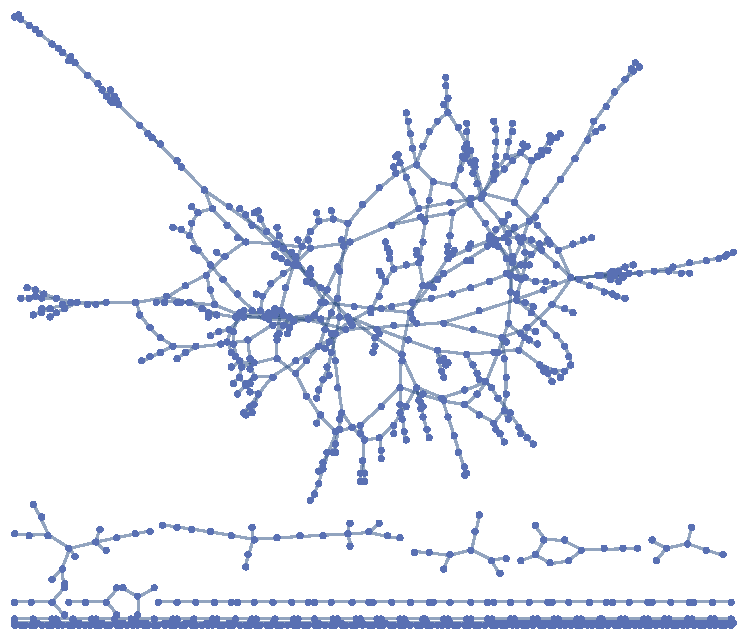
\includegraphics[page=1,width=.31\textwidth]{figures/chapter1/ER_1000_5}}%
	\caption{Realizations of the Erd\H{o}s-Rényi random graph on $n=1000$ vertices with varying $\lambda = n \p$.}%
	\label{F: ER lambda}%
\end{figure}

Figure~\ref{F: ER lambda} provides two realizations of the random graph with different $\lambda$,
one subcritical and one supercritical.
Note how the largest connected components in the subcritical graph still consist of very few vertices
(the largest component here having 9 vertices, while $\log(1000) \approx 6.9$)
and how a lot of nodes are isolated.
In contrast, the supercritical graph features a single large component 
and all other components are either drastically smaller in size or even still isolated vertices.

\bigskip

For $n \p < 1$ we expect many small clusters of order at most $\log n$,
for $n \p > 1$ we expect one giant component, approaching size $n$ with increasing $\p$.
But what happens around $n \p \approx 1$?
As it turns out, the emergence of the giant component occurs quite rapidly,
such that shortly after $n \p = 1$ most graphs do not have any component of order between $\frac{1}{2}\n{2}{3}$ and $\n{2}{3}$.

The following theorem provides an approximation of the time of emergence of the giant component,
seeing the random graph on $n$ vertices as a graph process,
starting at $t=0$ with $0$ edges, adding one random edge at every time step.
We would therefore expect the emergence starting around time $\binom{2}{n}\frac{1}{n} \approx \frac{1}{2}n$.
We say a property $P$ is shared by almost every graph if the probability of having this property approaches $1$ as $n \rightarrow \infty$.

\begin{theorem}[Emergence of the giant component, {\cite[Theorem 6.8, p.142]{Bollobas.2001}}]
	Almost every graph process
	$\Gcal = (\Gcal_t)_0^n$ is such that 
	for every $t \geq t_1 = \floor{ n/2 + 2(\log n)^{1/2}\n{2}{3} }$ 
	the graph $\Gcal_t$ has a unique component of order at least $\n{2}{3}$ and the other components have at most $\frac{1}{2}\n{2}{3}$.
\end{theorem}

As it turns out, there is a so-called critical window in which the maximum component sizes are not of order $\log n$ any more 
but there is no single giant component yet.
We call a random graph $\Gcal(n, n^{-1} + \pp\n{-4}{3})$ critical for $\pp \in \Real$.\label{I: pp}
The next theorem provides a approximation of the size of the largest component in a critical random graph.

\begin{theorem}[Largest critical cluster, {\cite[Theorem 5.1, p.150]{vanderHofstad.2016}}] \label{T: largest critical cluster}
	Let $\lambda = 1 + \pp\n{-1}{3}$, with $\pp \in \Real$.
	There exists a constant $b = b(\pp)$ such that for all $\omega > 1$,
	\begin{equation}
		\Prob\left( \omega^{-1} \n{2}{3} \leq |\Ccal_{\max}| \leq \omega \n{2}{3}\right) \geq 1 - \frac{b}{\omega}.
	\end{equation}	
\end{theorem}

In this critical window, the largest component of the random graph will be of order $\n{2}{3}$ with high probability.

\begin{figure}[h]
	\centering
	\subfloat[$\pp = -3$]{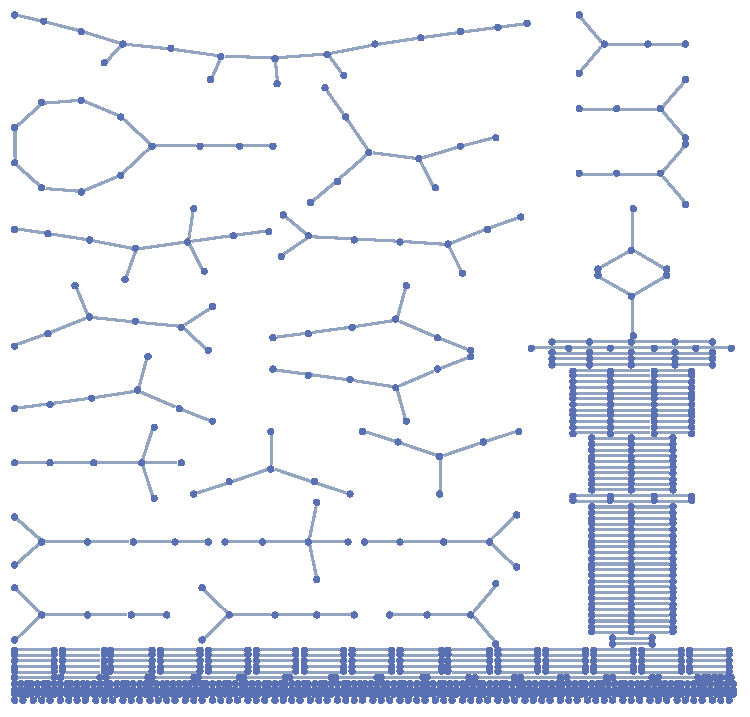
\includegraphics[page=1,width=.31\textwidth]{figures/chapter1/ER_1000_-3}}%
	\quad
	\subfloat[$\pp = 0$]{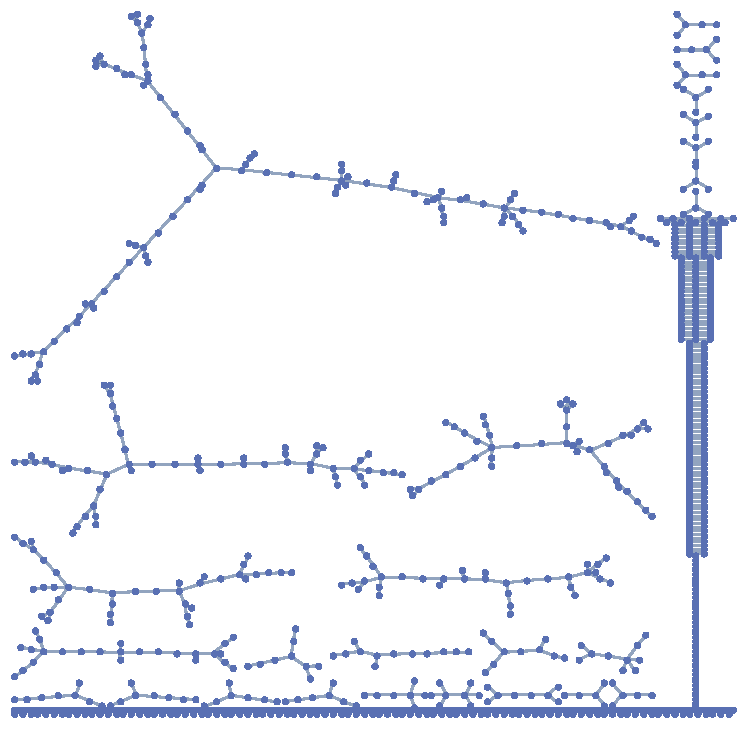
\includegraphics[page=1,width=.31\textwidth]{figures/chapter1/ER_1000_1}}%
	\quad
	\subfloat[$\pp = 3$]{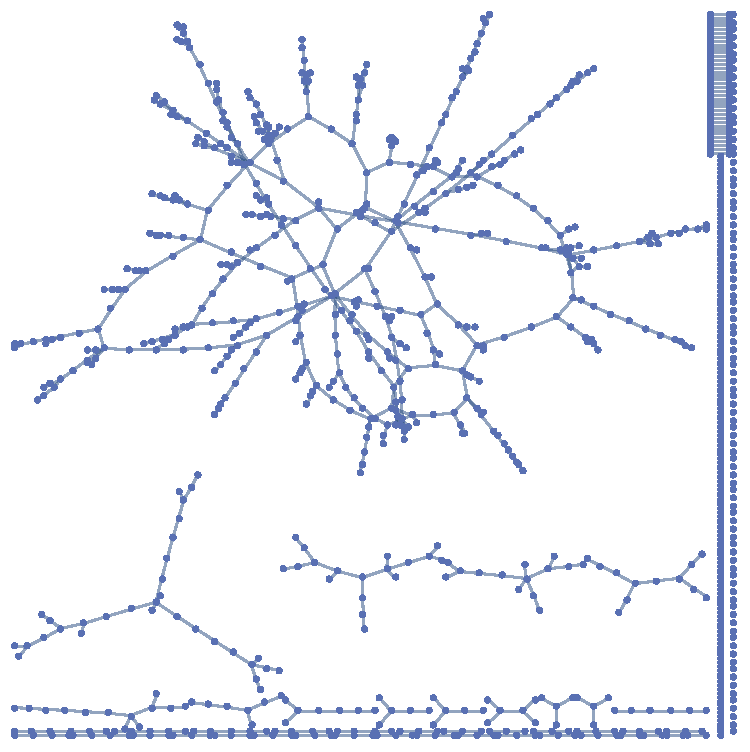
\includegraphics[page=1,width=.31\textwidth]{figures/chapter1/ER_1000_3}}%
	\caption{Realizations of the Erd\H{o}s-Rényi random graph on $n=1000$ vertices with varying $\pp$.}%
	\label{F: ER p}%
\end{figure}

Figure~\ref{F: ER p} shows realizations of the critical Erd\H{o}s-Rényi random graph for different parameters $\pp$.
It is evident how the graph undergoes its transition from relatively small and simple components 
to the emergence of a single great component, which will later, i.e. for larger $\p$,
encompass more and more vertices as seen in Figure~\ref{F: ER lambda}.

\bigskip

But is it possible to provide a similar statement not only for the largest, but for all components in a critical random graph?
Aldous notes that previous to his paper
the convergence of the rescaled component sizes to some limit process was generally assumed to be true,
although never explicitly proven.
He therefore provides the following folk theorem,
which will be proven along with a more precise version in the course of this thesis.

For a connected component we define the number of surplus edges or the surplus by
\begin{equation}
	\text{surplus} = \text{number of edges} - \text{number of vertices} + 1.
\end{equation}
The surplus gives the maximum number of edges we can remove from the component so that it stays connected.
A component with a surplus of zero is a tree.

\begin{folktheorem} \label{T: folk theorem}
	Let $\Cnt(1) \geq \Cnt(2) \geq \dots$ be the ordered component sizes of
	$\Gcal(n, n^{-1} + \pp\n{-4}{3})$ and let $\sigmant(j)$ be the surplus of the corresponding component.
	Then
	\begin{equation}
		( \n{-2}{3} ( \Cnt(j), \sigmant(j) ), \; j \geq 1 ) 
		\rightarrow_d
		( (\Ct(j), \sigmat(j)), \; j \geq 1 )
		= ( \Ctbold, \sigmatbold ),
	\end{equation}
	as $n \rightarrow \infty$ for some limit $( \Ctbold, \sigmatbold )$
	with $0 < \Ct(j) < \infty$ and $0 \leq \sigmat(j) < \infty$ almost surely for each $j \geq 1$.
\end{folktheorem}

The convergence is to hold with respect to the product topology, 
where $\xn \rightarrow \x$ holds for $\xn = (x^{(n)}_1, x^{(n)}_2, \dots)$ and $\x = (x_1, x_2, \dots)$
if for all $k \in \Nat$
\begin{equation}
	(x^{(n)}_1, \dots, x^{(n)}_k) \rightarrow (x_1, \dots,  x_k)
\end{equation}
by $x^{(n)}_i \rightarrow x_i$ for all $1 \leq i \leq k$ as $n \rightarrow \infty$.
Note that in our theorem the $x^{(n)}_i = ( \n{-2}{3} \Cnt(i), \n{-2}{3} \sigmant(i))$ and $x_i = (\Ct(i), \sigmat(i))$ are pairs of values themselves,
so for $x^{(n)}_i \rightarrow x_i$ to hold we require 
$\n{-2}{3}  \Cnt(i) \rightarrow \Ct(i)$ and $\n{-2}{3} \sigmant(i) \rightarrow \sigmat(i)$ 
in $\Real$ as $n \rightarrow \infty$.


\section{Main statements of this thesis}
%%%%%%%%%%%%%%%%%%%%%%%%%%%%%%%%%%%%%%%%%%%%%%%%%%%%%%%%%%%%
% SECTION: Main statements of this thesis
%%%%%%%%%%%%%%%%%%%%%%%%%%%%%%%%%%%%%%%%%%%%%%%%%%%%%%%%%%%%

In this section we state the main results of this thesis,
which is a refinement of Folk Theorem~\ref{T: folk theorem}.
We now identify the distribution of the limit vector precisely and state a stricter form of convergence of component sizes.

Denote by $W$ the standard Brownian motion on $\Rplus$.\label{I: bm} 
For a fixed parameter $\pp \in \Real$ we call the process $\Wt$, defined by
\begin{equation} \label{D: Wt}
	\Wt(s) := W(s) + \int_{0}^{s}(\pp - u)du = W(s) + \pp s - \frac{1}{2}s^2,
\end{equation}
the Brownian motion with drift $\pp -s$ at time $s$.
The central object of our analysis will be the process $\Wt$ and its excursions above past minima.
We reflect $\Wt$ at the x-axis to define the process $\Bt$ by
\begin{equation} \label{D: Bt}
	\Bt(s) := \Wt(s) - \min_{u \leq s}\Wt(u).
\end{equation}
We call $\Bt$ the reflected Brownian motion with drift.

\begin{figure}[h]%
	\centering
	\subfloat[$W(s)$]{% Created by tikzDevice version 0.10.1 on 2017-05-10 12:46:18
% !TEX encoding = UTF-8 Unicode
\begin{tikzpicture}[x=1pt,y=1pt]
\definecolor{fillColor}{RGB}{255,255,255}
\path[use as bounding box,fill=fillColor,fill opacity=0.00] (0,0) rectangle (108.41,108.41);
\begin{scope}
\path[clip] (  0.00,  0.00) rectangle (108.40,108.41);
\definecolor{drawColor}{RGB}{255,255,255}
\definecolor{fillColor}{RGB}{255,255,255}

\path[draw=drawColor,line width= 0.6pt,line join=round,line cap=round,fill=fillColor] (  0.00,  0.00) rectangle (108.41,108.41);
\end{scope}
\begin{scope}
\path[clip] (  9.00,  9.00) rectangle (102.41,102.41);
\definecolor{fillColor}{RGB}{255,255,255}

\path[fill=fillColor] (  9.00,  9.00) rectangle (102.40,102.41);
\definecolor{drawColor}{gray}{0.98}

\path[draw=drawColor,line width= 0.6pt,line join=round] (  9.00, 27.33) --
	(102.41, 27.33);

\path[draw=drawColor,line width= 0.6pt,line join=round] (  9.00, 53.68) --
	(102.41, 53.68);

\path[draw=drawColor,line width= 0.6pt,line join=round] (  9.00, 80.02) --
	(102.41, 80.02);

\path[draw=drawColor,line width= 0.6pt,line join=round] ( 23.86,  9.00) --
	( 23.86,102.41);

\path[draw=drawColor,line width= 0.6pt,line join=round] ( 45.09,  9.00) --
	( 45.09,102.41);

\path[draw=drawColor,line width= 0.6pt,line join=round] ( 66.32,  9.00) --
	( 66.32,102.41);

\path[draw=drawColor,line width= 0.6pt,line join=round] ( 87.55,  9.00) --
	( 87.55,102.41);
\definecolor{drawColor}{gray}{0.90}

\path[draw=drawColor,line width= 0.2pt,line join=round] (  9.00, 14.16) --
	(102.41, 14.16);

\path[draw=drawColor,line width= 0.2pt,line join=round] (  9.00, 40.51) --
	(102.41, 40.51);

\path[draw=drawColor,line width= 0.2pt,line join=round] (  9.00, 66.85) --
	(102.41, 66.85);

\path[draw=drawColor,line width= 0.2pt,line join=round] (  9.00, 93.20) --
	(102.41, 93.20);

\path[draw=drawColor,line width= 0.2pt,line join=round] ( 13.25,  9.00) --
	( 13.25,102.41);

\path[draw=drawColor,line width= 0.2pt,line join=round] ( 34.47,  9.00) --
	( 34.47,102.41);

\path[draw=drawColor,line width= 0.2pt,line join=round] ( 55.70,  9.00) --
	( 55.70,102.41);

\path[draw=drawColor,line width= 0.2pt,line join=round] ( 76.93,  9.00) --
	( 76.93,102.41);

\path[draw=drawColor,line width= 0.2pt,line join=round] ( 98.16,  9.00) --
	( 98.16,102.41);
\definecolor{drawColor}{RGB}{0,0,0}

\path[draw=drawColor,line width= 0.3pt,line join=round] ( 13.25, 66.85) --
	( 13.29, 65.53) --
	( 13.33, 65.77) --
	( 13.37, 66.53) --
	( 13.42, 66.35) --
	( 13.46, 66.33) --
	( 13.50, 66.35) --
	( 13.54, 64.91) --
	( 13.59, 62.96) --
	( 13.63, 63.01) --
	( 13.67, 61.39) --
	( 13.71, 61.32) --
	( 13.76, 60.98) --
	( 13.80, 58.33) --
	( 13.84, 57.98) --
	( 13.88, 58.44) --
	( 13.92, 58.91) --
	( 13.97, 57.65) --
	( 14.01, 59.52) --
	( 14.05, 60.34) --
	( 14.09, 60.18) --
	( 14.14, 59.86) --
	( 14.18, 62.08) --
	( 14.22, 62.00) --
	( 14.26, 62.75) --
	( 14.31, 61.75) --
	( 14.35, 61.57) --
	( 14.39, 62.10) --
	( 14.43, 62.33) --
	( 14.48, 62.65) --
	( 14.52, 64.43) --
	( 14.56, 63.67) --
	( 14.60, 64.76) --
	( 14.65, 62.59) --
	( 14.69, 63.10) --
	( 14.73, 64.09) --
	( 14.77, 64.61) --
	( 14.82, 64.82) --
	( 14.86, 64.03) --
	( 14.90, 64.20) --
	( 14.94, 64.98) --
	( 14.99, 63.69) --
	( 15.03, 67.02) --
	( 15.07, 68.66) --
	( 15.11, 68.86) --
	( 15.16, 67.07) --
	( 15.20, 66.63) --
	( 15.24, 67.36) --
	( 15.28, 69.02) --
	( 15.33, 69.74) --
	( 15.37, 69.35) --
	( 15.41, 68.96) --
	( 15.45, 68.83) --
	( 15.50, 68.66) --
	( 15.54, 67.01) --
	( 15.58, 68.24) --
	( 15.62, 67.59) --
	( 15.67, 68.55) --
	( 15.71, 66.88) --
	( 15.75, 65.67) --
	( 15.79, 66.09) --
	( 15.84, 67.54) --
	( 15.88, 69.50) --
	( 15.92, 70.11) --
	( 15.96, 71.15) --
	( 16.01, 70.89) --
	( 16.05, 67.90) --
	( 16.09, 66.46) --
	( 16.13, 66.96) --
	( 16.18, 68.15) --
	( 16.22, 69.19) --
	( 16.26, 68.50) --
	( 16.30, 69.29) --
	( 16.35, 69.60) --
	( 16.39, 69.25) --
	( 16.43, 68.06) --
	( 16.47, 68.12) --
	( 16.51, 66.80) --
	( 16.56, 64.38) --
	( 16.60, 65.59) --
	( 16.64, 66.05) --
	( 16.68, 65.94) --
	( 16.73, 66.41) --
	( 16.77, 67.21) --
	( 16.81, 67.51) --
	( 16.85, 66.64) --
	( 16.90, 68.61) --
	( 16.94, 70.28) --
	( 16.98, 69.03) --
	( 17.02, 69.84) --
	( 17.07, 69.00) --
	( 17.11, 68.21) --
	( 17.15, 68.12) --
	( 17.19, 68.47) --
	( 17.24, 69.15) --
	( 17.28, 69.14) --
	( 17.32, 72.30) --
	( 17.36, 74.80) --
	( 17.41, 75.58) --
	( 17.45, 75.03) --
	( 17.49, 73.62) --
	( 17.53, 71.24) --
	( 17.58, 70.96) --
	( 17.62, 70.16) --
	( 17.66, 69.00) --
	( 17.70, 67.62) --
	( 17.75, 67.59) --
	( 17.79, 67.08) --
	( 17.83, 66.45) --
	( 17.87, 67.76) --
	( 17.92, 68.57) --
	( 17.96, 68.05) --
	( 18.00, 68.53) --
	( 18.04, 68.81) --
	( 18.09, 68.58) --
	( 18.13, 68.54) --
	( 18.17, 70.96) --
	( 18.21, 71.74) --
	( 18.26, 71.18) --
	( 18.30, 71.81) --
	( 18.34, 71.91) --
	( 18.38, 72.81) --
	( 18.43, 72.40) --
	( 18.47, 71.57) --
	( 18.51, 70.90) --
	( 18.55, 71.73) --
	( 18.60, 70.05) --
	( 18.64, 69.08) --
	( 18.68, 68.90) --
	( 18.72, 68.13) --
	( 18.77, 68.67) --
	( 18.81, 66.85) --
	( 18.85, 67.08) --
	( 18.89, 68.15) --
	( 18.93, 68.86) --
	( 18.98, 68.74) --
	( 19.02, 68.68) --
	( 19.06, 67.22) --
	( 19.10, 67.99) --
	( 19.15, 67.10) --
	( 19.19, 68.38) --
	( 19.23, 67.74) --
	( 19.27, 67.78) --
	( 19.32, 68.84) --
	( 19.36, 69.72) --
	( 19.40, 68.98) --
	( 19.44, 69.28) --
	( 19.49, 68.77) --
	( 19.53, 71.64) --
	( 19.57, 71.31) --
	( 19.61, 70.63) --
	( 19.66, 71.60) --
	( 19.70, 69.88) --
	( 19.74, 70.32) --
	( 19.78, 70.49) --
	( 19.83, 68.77) --
	( 19.87, 69.36) --
	( 19.91, 68.44) --
	( 19.95, 67.19) --
	( 20.00, 67.56) --
	( 20.04, 68.00) --
	( 20.08, 68.61) --
	( 20.12, 70.35) --
	( 20.17, 69.77) --
	( 20.21, 69.84) --
	( 20.25, 69.59) --
	( 20.29, 68.82) --
	( 20.34, 68.89) --
	( 20.38, 69.18) --
	( 20.42, 68.59) --
	( 20.46, 69.07) --
	( 20.51, 69.07) --
	( 20.55, 67.58) --
	( 20.59, 68.46) --
	( 20.63, 65.94) --
	( 20.68, 65.85) --
	( 20.72, 65.61) --
	( 20.76, 63.80) --
	( 20.80, 60.78) --
	( 20.85, 62.61) --
	( 20.89, 60.03) --
	( 20.93, 59.93) --
	( 20.97, 60.30) --
	( 21.02, 59.38) --
	( 21.06, 58.67) --
	( 21.10, 58.30) --
	( 21.14, 57.71) --
	( 21.19, 57.34) --
	( 21.23, 56.64) --
	( 21.27, 56.55) --
	( 21.31, 56.03) --
	( 21.35, 59.81) --
	( 21.40, 62.79) --
	( 21.44, 63.17) --
	( 21.48, 62.28) --
	( 21.52, 63.32) --
	( 21.57, 65.10) --
	( 21.61, 65.92) --
	( 21.65, 65.80) --
	( 21.69, 65.05) --
	( 21.74, 65.28) --
	( 21.78, 65.43) --
	( 21.82, 67.02) --
	( 21.86, 65.82) --
	( 21.91, 66.88) --
	( 21.95, 65.63) --
	( 21.99, 66.37) --
	( 22.03, 66.48) --
	( 22.08, 66.44) --
	( 22.12, 67.44) --
	( 22.16, 66.17) --
	( 22.20, 65.83) --
	( 22.25, 65.45) --
	( 22.29, 68.70) --
	( 22.33, 68.41) --
	( 22.37, 69.63) --
	( 22.42, 68.37) --
	( 22.46, 66.97) --
	( 22.50, 69.20) --
	( 22.54, 68.96) --
	( 22.59, 69.23) --
	( 22.63, 69.70) --
	( 22.67, 68.74) --
	( 22.71, 67.88) --
	( 22.76, 66.35) --
	( 22.80, 66.86) --
	( 22.84, 67.49) --
	( 22.88, 67.62) --
	( 22.93, 67.04) --
	( 22.97, 67.51) --
	( 23.01, 69.84) --
	( 23.05, 68.85) --
	( 23.10, 67.60) --
	( 23.14, 67.93) --
	( 23.18, 67.02) --
	( 23.22, 66.77) --
	( 23.27, 66.51) --
	( 23.31, 68.11) --
	( 23.35, 65.38) --
	( 23.39, 62.78) --
	( 23.44, 64.24) --
	( 23.48, 63.71) --
	( 23.52, 64.25) --
	( 23.56, 65.82) --
	( 23.61, 66.55) --
	( 23.65, 65.20) --
	( 23.69, 64.91) --
	( 23.73, 62.88) --
	( 23.77, 63.85) --
	( 23.82, 63.45) --
	( 23.86, 62.84) --
	( 23.90, 63.32) --
	( 23.94, 62.72) --
	( 23.99, 62.66) --
	( 24.03, 61.74) --
	( 24.07, 60.21) --
	( 24.11, 59.99) --
	( 24.16, 60.14) --
	( 24.20, 59.72) --
	( 24.24, 60.14) --
	( 24.28, 58.25) --
	( 24.33, 60.96) --
	( 24.37, 60.27) --
	( 24.41, 58.64) --
	( 24.45, 58.42) --
	( 24.50, 57.70) --
	( 24.54, 58.55) --
	( 24.58, 57.31) --
	( 24.62, 57.76) --
	( 24.67, 58.18) --
	( 24.71, 57.22) --
	( 24.75, 56.33) --
	( 24.79, 56.87) --
	( 24.84, 57.18) --
	( 24.88, 58.16) --
	( 24.92, 56.84) --
	( 24.96, 56.48) --
	( 25.01, 57.20) --
	( 25.05, 57.09) --
	( 25.09, 55.14) --
	( 25.13, 53.91) --
	( 25.18, 54.31) --
	( 25.22, 52.51) --
	( 25.26, 52.51) --
	( 25.30, 51.47) --
	( 25.35, 51.21) --
	( 25.39, 50.09) --
	( 25.43, 48.59) --
	( 25.47, 46.99) --
	( 25.52, 47.26) --
	( 25.56, 47.52) --
	( 25.60, 48.14) --
	( 25.64, 49.08) --
	( 25.69, 52.07) --
	( 25.73, 51.05) --
	( 25.77, 49.74) --
	( 25.81, 50.55) --
	( 25.86, 48.10) --
	( 25.90, 48.31) --
	( 25.94, 48.05) --
	( 25.98, 48.76) --
	( 26.03, 47.68) --
	( 26.07, 47.07) --
	( 26.11, 47.21) --
	( 26.15, 47.02) --
	( 26.20, 48.55) --
	( 26.24, 47.33) --
	( 26.28, 45.57) --
	( 26.32, 46.38) --
	( 26.36, 46.80) --
	( 26.41, 45.98) --
	( 26.45, 44.92) --
	( 26.49, 47.53) --
	( 26.53, 48.19) --
	( 26.58, 48.08) --
	( 26.62, 48.78) --
	( 26.66, 48.60) --
	( 26.70, 47.60) --
	( 26.75, 46.27) --
	( 26.79, 46.88) --
	( 26.83, 47.57) --
	( 26.87, 46.77) --
	( 26.92, 46.16) --
	( 26.96, 45.27) --
	( 27.00, 47.12) --
	( 27.04, 46.76) --
	( 27.09, 45.68) --
	( 27.13, 46.66) --
	( 27.17, 45.84) --
	( 27.21, 44.90) --
	( 27.26, 45.13) --
	( 27.30, 41.65) --
	( 27.34, 38.33) --
	( 27.38, 38.45) --
	( 27.43, 39.97) --
	( 27.47, 41.11) --
	( 27.51, 41.39) --
	( 27.55, 41.75) --
	( 27.60, 42.30) --
	( 27.64, 41.89) --
	( 27.68, 42.30) --
	( 27.72, 43.58) --
	( 27.77, 41.79) --
	( 27.81, 41.71) --
	( 27.85, 41.43) --
	( 27.89, 42.42) --
	( 27.94, 40.37) --
	( 27.98, 38.79) --
	( 28.02, 38.57) --
	( 28.06, 39.20) --
	( 28.11, 40.14) --
	( 28.15, 41.14) --
	( 28.19, 40.48) --
	( 28.23, 40.39) --
	( 28.28, 40.22) --
	( 28.32, 41.39) --
	( 28.36, 41.55) --
	( 28.40, 43.67) --
	( 28.45, 42.27) --
	( 28.49, 41.63) --
	( 28.53, 40.50) --
	( 28.57, 38.31) --
	( 28.62, 40.54) --
	( 28.66, 38.08) --
	( 28.70, 38.10) --
	( 28.74, 37.27) --
	( 28.78, 37.45) --
	( 28.83, 36.65) --
	( 28.87, 38.40) --
	( 28.91, 40.03) --
	( 28.95, 40.96) --
	( 29.00, 39.41) --
	( 29.04, 38.70) --
	( 29.08, 37.08) --
	( 29.12, 36.92) --
	( 29.17, 38.42) --
	( 29.21, 38.28) --
	( 29.25, 39.05) --
	( 29.29, 38.03) --
	( 29.34, 38.09) --
	( 29.38, 36.97) --
	( 29.42, 35.71) --
	( 29.46, 37.85) --
	( 29.51, 37.06) --
	( 29.55, 35.75) --
	( 29.59, 35.16) --
	( 29.63, 37.20) --
	( 29.68, 36.76) --
	( 29.72, 35.32) --
	( 29.76, 34.65) --
	( 29.80, 35.79) --
	( 29.85, 34.89) --
	( 29.89, 34.33) --
	( 29.93, 34.17) --
	( 29.97, 32.39) --
	( 30.02, 31.77) --
	( 30.06, 30.04) --
	( 30.10, 31.61) --
	( 30.14, 33.14) --
	( 30.19, 34.80) --
	( 30.23, 33.20) --
	( 30.27, 33.28) --
	( 30.31, 34.23) --
	( 30.36, 34.21) --
	( 30.40, 32.70) --
	( 30.44, 33.45) --
	( 30.48, 33.89) --
	( 30.53, 33.25) --
	( 30.57, 32.55) --
	( 30.61, 32.58) --
	( 30.65, 33.12) --
	( 30.70, 31.92) --
	( 30.74, 33.16) --
	( 30.78, 33.98) --
	( 30.82, 34.39) --
	( 30.87, 34.02) --
	( 30.91, 33.13) --
	( 30.95, 32.91) --
	( 30.99, 33.49) --
	( 31.04, 34.21) --
	( 31.08, 33.25) --
	( 31.12, 32.81) --
	( 31.16, 33.15) --
	( 31.20, 32.24) --
	( 31.25, 32.19) --
	( 31.29, 31.12) --
	( 31.33, 31.21) --
	( 31.37, 31.23) --
	( 31.42, 32.78) --
	( 31.46, 33.57) --
	( 31.50, 33.61) --
	( 31.54, 33.28) --
	( 31.59, 34.35) --
	( 31.63, 33.36) --
	( 31.67, 33.73) --
	( 31.71, 34.01) --
	( 31.76, 35.20) --
	( 31.80, 35.39) --
	( 31.84, 35.20) --
	( 31.88, 36.42) --
	( 31.93, 36.86) --
	( 31.97, 36.77) --
	( 32.01, 38.22) --
	( 32.05, 39.22) --
	( 32.10, 38.92) --
	( 32.14, 39.65) --
	( 32.18, 39.66) --
	( 32.22, 38.04) --
	( 32.27, 36.33) --
	( 32.31, 36.93) --
	( 32.35, 38.04) --
	( 32.39, 39.02) --
	( 32.44, 39.90) --
	( 32.48, 40.19) --
	( 32.52, 43.45) --
	( 32.56, 43.23) --
	( 32.61, 42.89) --
	( 32.65, 42.80) --
	( 32.69, 44.60) --
	( 32.73, 46.35) --
	( 32.78, 47.97) --
	( 32.82, 47.06) --
	( 32.86, 48.82) --
	( 32.90, 48.84) --
	( 32.95, 49.23) --
	( 32.99, 48.08) --
	( 33.03, 46.59) --
	( 33.07, 46.61) --
	( 33.12, 47.44) --
	( 33.16, 46.76) --
	( 33.20, 47.01) --
	( 33.24, 46.71) --
	( 33.29, 46.60) --
	( 33.33, 47.55) --
	( 33.37, 43.67) --
	( 33.41, 43.87) --
	( 33.46, 44.96) --
	( 33.50, 44.76) --
	( 33.54, 47.82) --
	( 33.58, 46.50) --
	( 33.62, 47.03) --
	( 33.67, 45.33) --
	( 33.71, 44.94) --
	( 33.75, 44.39) --
	( 33.79, 46.44) --
	( 33.84, 45.31) --
	( 33.88, 44.55) --
	( 33.92, 43.08) --
	( 33.96, 43.99) --
	( 34.01, 43.64) --
	( 34.05, 43.71) --
	( 34.09, 44.94) --
	( 34.13, 45.46) --
	( 34.18, 44.78) --
	( 34.22, 46.80) --
	( 34.26, 47.93) --
	( 34.30, 47.57) --
	( 34.35, 47.46) --
	( 34.39, 48.58) --
	( 34.43, 49.67) --
	( 34.47, 50.09) --
	( 34.52, 51.65) --
	( 34.56, 50.06) --
	( 34.60, 50.61) --
	( 34.64, 50.56) --
	( 34.69, 51.32) --
	( 34.73, 52.30) --
	( 34.77, 52.86) --
	( 34.81, 53.82) --
	( 34.86, 53.17) --
	( 34.90, 53.91) --
	( 34.94, 53.82) --
	( 34.98, 52.84) --
	( 35.03, 50.73) --
	( 35.07, 52.74) --
	( 35.11, 53.39) --
	( 35.15, 52.88) --
	( 35.20, 51.78) --
	( 35.24, 50.92) --
	( 35.28, 51.41) --
	( 35.32, 51.75) --
	( 35.37, 51.38) --
	( 35.41, 50.09) --
	( 35.45, 52.21) --
	( 35.49, 55.35) --
	( 35.54, 53.82) --
	( 35.58, 53.32) --
	( 35.62, 52.92) --
	( 35.66, 55.69) --
	( 35.71, 58.03) --
	( 35.75, 59.20) --
	( 35.79, 59.47) --
	( 35.83, 59.19) --
	( 35.88, 60.48) --
	( 35.92, 60.68) --
	( 35.96, 60.92) --
	( 36.00, 62.37) --
	( 36.04, 59.47) --
	( 36.09, 60.20) --
	( 36.13, 61.28) --
	( 36.17, 60.74) --
	( 36.21, 61.51) --
	( 36.26, 61.77) --
	( 36.30, 61.29) --
	( 36.34, 61.10) --
	( 36.38, 62.08) --
	( 36.43, 61.24) --
	( 36.47, 62.46) --
	( 36.51, 59.33) --
	( 36.55, 60.51) --
	( 36.60, 60.29) --
	( 36.64, 60.46) --
	( 36.68, 60.51) --
	( 36.72, 61.79) --
	( 36.77, 62.05) --
	( 36.81, 62.49) --
	( 36.85, 63.54) --
	( 36.89, 64.22) --
	( 36.94, 66.83) --
	( 36.98, 68.05) --
	( 37.02, 66.23) --
	( 37.06, 66.55) --
	( 37.11, 67.79) --
	( 37.15, 68.92) --
	( 37.19, 67.02) --
	( 37.23, 69.73) --
	( 37.28, 70.42) --
	( 37.32, 71.29) --
	( 37.36, 72.07) --
	( 37.40, 71.29) --
	( 37.45, 72.66) --
	( 37.49, 73.22) --
	( 37.53, 73.39) --
	( 37.57, 72.09) --
	( 37.62, 69.46) --
	( 37.66, 68.56) --
	( 37.70, 67.13) --
	( 37.74, 66.86) --
	( 37.79, 67.31) --
	( 37.83, 67.36) --
	( 37.87, 66.11) --
	( 37.91, 66.55) --
	( 37.96, 65.64) --
	( 38.00, 67.34) --
	( 38.04, 69.30) --
	( 38.08, 68.29) --
	( 38.13, 66.63) --
	( 38.17, 65.76) --
	( 38.21, 64.79) --
	( 38.25, 65.61) --
	( 38.30, 64.34) --
	( 38.34, 64.11) --
	( 38.38, 64.52) --
	( 38.42, 64.19) --
	( 38.47, 64.15) --
	( 38.51, 64.22) --
	( 38.55, 65.38) --
	( 38.59, 67.62) --
	( 38.63, 68.38) --
	( 38.68, 65.77) --
	( 38.72, 66.80) --
	( 38.76, 64.64) --
	( 38.80, 65.59) --
	( 38.85, 66.43) --
	( 38.89, 66.92) --
	( 38.93, 66.76) --
	( 38.97, 64.53) --
	( 39.02, 65.23) --
	( 39.06, 65.65) --
	( 39.10, 65.58) --
	( 39.14, 64.71) --
	( 39.19, 65.04) --
	( 39.23, 67.46) --
	( 39.27, 68.66) --
	( 39.31, 68.03) --
	( 39.36, 68.94) --
	( 39.40, 67.61) --
	( 39.44, 65.85) --
	( 39.48, 64.85) --
	( 39.53, 65.38) --
	( 39.57, 64.12) --
	( 39.61, 64.10) --
	( 39.65, 65.43) --
	( 39.70, 63.84) --
	( 39.74, 62.70) --
	( 39.78, 63.55) --
	( 39.82, 61.89) --
	( 39.87, 59.92) --
	( 39.91, 58.44) --
	( 39.95, 59.14) --
	( 39.99, 58.04) --
	( 40.04, 58.23) --
	( 40.08, 58.72) --
	( 40.12, 59.70) --
	( 40.16, 59.95) --
	( 40.21, 60.97) --
	( 40.25, 60.87) --
	( 40.29, 62.08) --
	( 40.33, 61.16) --
	( 40.38, 61.37) --
	( 40.42, 61.37) --
	( 40.46, 60.73) --
	( 40.50, 61.66) --
	( 40.55, 60.64) --
	( 40.59, 61.25) --
	( 40.63, 59.58) --
	( 40.67, 57.50) --
	( 40.72, 59.40) --
	( 40.76, 57.48) --
	( 40.80, 56.99) --
	( 40.84, 56.69) --
	( 40.89, 57.50) --
	( 40.93, 57.80) --
	( 40.97, 57.58) --
	( 41.01, 59.05) --
	( 41.05, 58.31) --
	( 41.10, 59.39) --
	( 41.14, 59.85) --
	( 41.18, 60.67) --
	( 41.22, 60.31) --
	( 41.27, 58.75) --
	( 41.31, 59.55) --
	( 41.35, 60.30) --
	( 41.39, 62.38) --
	( 41.44, 60.80) --
	( 41.48, 60.25) --
	( 41.52, 60.63) --
	( 41.56, 60.55) --
	( 41.61, 60.33) --
	( 41.65, 60.16) --
	( 41.69, 60.25) --
	( 41.73, 60.20) --
	( 41.78, 60.38) --
	( 41.82, 60.14) --
	( 41.86, 59.60) --
	( 41.90, 59.64) --
	( 41.95, 60.15) --
	( 41.99, 61.01) --
	( 42.03, 62.60) --
	( 42.07, 64.96) --
	( 42.12, 66.83) --
	( 42.16, 67.21) --
	( 42.20, 69.56) --
	( 42.24, 70.81) --
	( 42.29, 71.93) --
	( 42.33, 71.71) --
	( 42.37, 71.11) --
	( 42.41, 72.57) --
	( 42.46, 73.41) --
	( 42.50, 75.02) --
	( 42.54, 76.86) --
	( 42.58, 78.15) --
	( 42.63, 77.14) --
	( 42.67, 77.00) --
	( 42.71, 76.25) --
	( 42.75, 74.42) --
	( 42.80, 74.84) --
	( 42.84, 77.39) --
	( 42.88, 77.90) --
	( 42.92, 79.81) --
	( 42.97, 80.09) --
	( 43.01, 77.95) --
	( 43.05, 77.38) --
	( 43.09, 78.73) --
	( 43.14, 78.89) --
	( 43.18, 81.34) --
	( 43.22, 82.30) --
	( 43.26, 82.39) --
	( 43.31, 83.04) --
	( 43.35, 85.27) --
	( 43.39, 83.93) --
	( 43.43, 83.03) --
	( 43.47, 84.10) --
	( 43.52, 84.06) --
	( 43.56, 83.17) --
	( 43.60, 82.55) --
	( 43.64, 82.52) --
	( 43.69, 80.74) --
	( 43.73, 82.68) --
	( 43.77, 83.49) --
	( 43.81, 83.44) --
	( 43.86, 84.09) --
	( 43.90, 85.16) --
	( 43.94, 87.61) --
	( 43.98, 86.26) --
	( 44.03, 85.86) --
	( 44.07, 85.34) --
	( 44.11, 86.10) --
	( 44.15, 86.76) --
	( 44.20, 87.28) --
	( 44.24, 86.78) --
	( 44.28, 85.48) --
	( 44.32, 84.74) --
	( 44.37, 82.55) --
	( 44.41, 83.84) --
	( 44.45, 85.05) --
	( 44.49, 85.48) --
	( 44.54, 86.17) --
	( 44.58, 84.51) --
	( 44.62, 84.73) --
	( 44.66, 84.05) --
	( 44.71, 83.98) --
	( 44.75, 85.18) --
	( 44.79, 86.17) --
	( 44.83, 85.30) --
	( 44.88, 84.58) --
	( 44.92, 85.21) --
	( 44.96, 84.11) --
	( 45.00, 84.02) --
	( 45.05, 84.57) --
	( 45.09, 84.65) --
	( 45.13, 85.02) --
	( 45.17, 86.17) --
	( 45.22, 86.74) --
	( 45.26, 86.67) --
	( 45.30, 88.83) --
	( 45.34, 87.37) --
	( 45.39, 87.82) --
	( 45.43, 84.81) --
	( 45.47, 84.77) --
	( 45.51, 85.25) --
	( 45.56, 85.43) --
	( 45.60, 85.49) --
	( 45.64, 86.91) --
	( 45.68, 88.21) --
	( 45.73, 90.10) --
	( 45.77, 89.70) --
	( 45.81, 89.52) --
	( 45.85, 91.52) --
	( 45.89, 91.07) --
	( 45.94, 91.85) --
	( 45.98, 91.13) --
	( 46.02, 92.04) --
	( 46.06, 91.82) --
	( 46.11, 91.25) --
	( 46.15, 91.78) --
	( 46.19, 93.02) --
	( 46.23, 91.30) --
	( 46.28, 92.24) --
	( 46.32, 92.52) --
	( 46.36, 93.97) --
	( 46.40, 95.03) --
	( 46.45, 97.51) --
	( 46.49, 96.76) --
	( 46.53, 98.16) --
	( 46.57, 97.23) --
	( 46.62, 95.77) --
	( 46.66, 95.81) --
	( 46.70, 94.83) --
	( 46.74, 93.86) --
	( 46.79, 93.15) --
	( 46.83, 92.82) --
	( 46.87, 93.48) --
	( 46.91, 94.23) --
	( 46.96, 94.59) --
	( 47.00, 93.25) --
	( 47.04, 93.52) --
	( 47.08, 95.55) --
	( 47.13, 95.64) --
	( 47.17, 97.09) --
	( 47.21, 95.82) --
	( 47.25, 95.78) --
	( 47.30, 94.99) --
	( 47.34, 96.80) --
	( 47.38, 97.15) --
	( 47.42, 96.12) --
	( 47.47, 95.37) --
	( 47.51, 95.03) --
	( 47.55, 94.97) --
	( 47.59, 92.59) --
	( 47.64, 92.36) --
	( 47.68, 91.11) --
	( 47.72, 89.17) --
	( 47.76, 90.41) --
	( 47.81, 91.51) --
	( 47.85, 91.06) --
	( 47.89, 91.74) --
	( 47.93, 91.64) --
	( 47.98, 89.93) --
	( 48.02, 89.46) --
	( 48.06, 87.13) --
	( 48.10, 85.93) --
	( 48.15, 87.90) --
	( 48.19, 87.09) --
	( 48.23, 88.51) --
	( 48.27, 87.66) --
	( 48.32, 88.83) --
	( 48.36, 86.52) --
	( 48.40, 88.46) --
	( 48.44, 89.49) --
	( 48.48, 90.73) --
	( 48.53, 92.41) --
	( 48.57, 89.82) --
	( 48.61, 87.24) --
	( 48.65, 85.30) --
	( 48.70, 85.03) --
	( 48.74, 84.02) --
	( 48.78, 83.40) --
	( 48.82, 82.90) --
	( 48.87, 84.84) --
	( 48.91, 85.72) --
	( 48.95, 87.07) --
	( 48.99, 86.95) --
	( 49.04, 86.98) --
	( 49.08, 87.07) --
	( 49.12, 89.11) --
	( 49.16, 89.18) --
	( 49.21, 89.74) --
	( 49.25, 91.67) --
	( 49.29, 94.61) --
	( 49.33, 92.39) --
	( 49.38, 91.93) --
	( 49.42, 90.86) --
	( 49.46, 89.97) --
	( 49.50, 89.58) --
	( 49.55, 89.46) --
	( 49.59, 87.86) --
	( 49.63, 86.22) --
	( 49.67, 86.37) --
	( 49.72, 84.82) --
	( 49.76, 84.77) --
	( 49.80, 84.43) --
	( 49.84, 83.81) --
	( 49.89, 83.77) --
	( 49.93, 83.97) --
	( 49.97, 81.59) --
	( 50.01, 80.38) --
	( 50.06, 81.87) --
	( 50.10, 84.00) --
	( 50.14, 83.25) --
	( 50.18, 82.64) --
	( 50.23, 83.39) --
	( 50.27, 82.46) --
	( 50.31, 82.65) --
	( 50.35, 82.60) --
	( 50.40, 83.88) --
	( 50.44, 84.17) --
	( 50.48, 83.48) --
	( 50.52, 80.97) --
	( 50.57, 81.99) --
	( 50.61, 82.77) --
	( 50.65, 82.14) --
	( 50.69, 82.87) --
	( 50.74, 80.68) --
	( 50.78, 83.02) --
	( 50.82, 82.64) --
	( 50.86, 83.10) --
	( 50.90, 82.39) --
	( 50.95, 82.82) --
	( 50.99, 80.39) --
	( 51.03, 80.38) --
	( 51.07, 79.70) --
	( 51.12, 80.27) --
	( 51.16, 80.33) --
	( 51.20, 81.22) --
	( 51.24, 82.96) --
	( 51.29, 83.00) --
	( 51.33, 82.21) --
	( 51.37, 80.00) --
	( 51.41, 79.39) --
	( 51.46, 77.30) --
	( 51.50, 76.67) --
	( 51.54, 76.81) --
	( 51.58, 76.12) --
	( 51.63, 75.18) --
	( 51.67, 73.90) --
	( 51.71, 72.04) --
	( 51.75, 73.10) --
	( 51.80, 73.09) --
	( 51.84, 74.17) --
	( 51.88, 72.75) --
	( 51.92, 71.31) --
	( 51.97, 70.66) --
	( 52.01, 71.56) --
	( 52.05, 72.27) --
	( 52.09, 73.37) --
	( 52.14, 74.71) --
	( 52.18, 74.57) --
	( 52.22, 76.36) --
	( 52.26, 75.83) --
	( 52.31, 75.58) --
	( 52.35, 74.98) --
	( 52.39, 75.62) --
	( 52.43, 79.04) --
	( 52.48, 80.32) --
	( 52.52, 78.78) --
	( 52.56, 78.03) --
	( 52.60, 78.76) --
	( 52.65, 79.70) --
	( 52.69, 79.44) --
	( 52.73, 78.34) --
	( 52.77, 79.40) --
	( 52.82, 79.52) --
	( 52.86, 79.42) --
	( 52.90, 79.38) --
	( 52.94, 79.66) --
	( 52.99, 81.42) --
	( 53.03, 79.63) --
	( 53.07, 78.80) --
	( 53.11, 78.33) --
	( 53.16, 80.19) --
	( 53.20, 80.03) --
	( 53.24, 79.72) --
	( 53.28, 79.09) --
	( 53.32, 78.96) --
	( 53.37, 78.97) --
	( 53.41, 81.31) --
	( 53.45, 82.01) --
	( 53.49, 81.87) --
	( 53.54, 80.98) --
	( 53.58, 79.89) --
	( 53.62, 81.35) --
	( 53.66, 80.79) --
	( 53.71, 79.43) --
	( 53.75, 77.57) --
	( 53.79, 79.05) --
	( 53.83, 79.39) --
	( 53.88, 80.34) --
	( 53.92, 81.19) --
	( 53.96, 80.93) --
	( 54.00, 80.13) --
	( 54.05, 81.07) --
	( 54.09, 82.63) --
	( 54.13, 83.90) --
	( 54.17, 81.24) --
	( 54.22, 79.77) --
	( 54.26, 79.25) --
	( 54.30, 77.95) --
	( 54.34, 78.26) --
	( 54.39, 77.00) --
	( 54.43, 76.71) --
	( 54.47, 76.80) --
	( 54.51, 75.95) --
	( 54.56, 75.66) --
	( 54.60, 76.74) --
	( 54.64, 74.15) --
	( 54.68, 72.74) --
	( 54.73, 72.96) --
	( 54.77, 71.12) --
	( 54.81, 70.34) --
	( 54.85, 68.54) --
	( 54.90, 67.20) --
	( 54.94, 65.95) --
	( 54.98, 65.22) --
	( 55.02, 65.34) --
	( 55.07, 66.01) --
	( 55.11, 65.72) --
	( 55.15, 64.97) --
	( 55.19, 65.36) --
	( 55.24, 62.34) --
	( 55.28, 62.43) --
	( 55.32, 62.61) --
	( 55.36, 63.90) --
	( 55.41, 63.33) --
	( 55.45, 63.49) --
	( 55.49, 60.45) --
	( 55.53, 60.86) --
	( 55.58, 59.48) --
	( 55.62, 61.44) --
	( 55.66, 61.70) --
	( 55.70, 62.00) --
	( 55.74, 60.47) --
	( 55.79, 61.79) --
	( 55.83, 61.13) --
	( 55.87, 62.42) --
	( 55.91, 62.17) --
	( 55.96, 59.91) --
	( 56.00, 60.16) --
	( 56.04, 58.64) --
	( 56.08, 59.04) --
	( 56.13, 58.34) --
	( 56.17, 59.47) --
	( 56.21, 61.07) --
	( 56.25, 59.36) --
	( 56.30, 60.57) --
	( 56.34, 59.60) --
	( 56.38, 57.70) --
	( 56.42, 58.74) --
	( 56.47, 59.00) --
	( 56.51, 60.23) --
	( 56.55, 59.62) --
	( 56.59, 61.90) --
	( 56.64, 61.41) --
	( 56.68, 59.60) --
	( 56.72, 60.34) --
	( 56.76, 62.42) --
	( 56.81, 58.75) --
	( 56.85, 57.88) --
	( 56.89, 57.52) --
	( 56.93, 58.69) --
	( 56.98, 57.88) --
	( 57.02, 58.16) --
	( 57.06, 60.42) --
	( 57.10, 58.94) --
	( 57.15, 58.84) --
	( 57.19, 59.64) --
	( 57.23, 59.08) --
	( 57.27, 58.05) --
	( 57.32, 59.05) --
	( 57.36, 59.35) --
	( 57.40, 58.34) --
	( 57.44, 60.37) --
	( 57.49, 60.81) --
	( 57.53, 61.91) --
	( 57.57, 61.84) --
	( 57.61, 61.42) --
	( 57.66, 57.17) --
	( 57.70, 56.75) --
	( 57.74, 58.75) --
	( 57.78, 56.37) --
	( 57.83, 58.00) --
	( 57.87, 56.99) --
	( 57.91, 56.27) --
	( 57.95, 55.78) --
	( 58.00, 56.01) --
	( 58.04, 56.16) --
	( 58.08, 55.97) --
	( 58.12, 57.08) --
	( 58.16, 58.83) --
	( 58.21, 57.02) --
	( 58.25, 56.82) --
	( 58.29, 57.76) --
	( 58.33, 58.28) --
	( 58.38, 57.91) --
	( 58.42, 56.23) --
	( 58.46, 57.55) --
	( 58.50, 57.37) --
	( 58.55, 56.38) --
	( 58.59, 56.40) --
	( 58.63, 56.76) --
	( 58.67, 56.29) --
	( 58.72, 56.86) --
	( 58.76, 55.94) --
	( 58.80, 55.45) --
	( 58.84, 54.67) --
	( 58.89, 54.48) --
	( 58.93, 54.59) --
	( 58.97, 54.57) --
	( 59.01, 55.95) --
	( 59.06, 54.02) --
	( 59.10, 54.95) --
	( 59.14, 56.28) --
	( 59.18, 55.18) --
	( 59.23, 54.89) --
	( 59.27, 54.52) --
	( 59.31, 55.91) --
	( 59.35, 55.04) --
	( 59.40, 52.77) --
	( 59.44, 51.25) --
	( 59.48, 51.55) --
	( 59.52, 50.65) --
	( 59.57, 50.14) --
	( 59.61, 50.84) --
	( 59.65, 51.15) --
	( 59.69, 51.29) --
	( 59.74, 51.27) --
	( 59.78, 49.32) --
	( 59.82, 48.37) --
	( 59.86, 46.32) --
	( 59.91, 46.36) --
	( 59.95, 44.15) --
	( 59.99, 45.02) --
	( 60.03, 46.31) --
	( 60.08, 47.25) --
	( 60.12, 47.09) --
	( 60.16, 48.32) --
	( 60.20, 47.81) --
	( 60.25, 46.12) --
	( 60.29, 45.21) --
	( 60.33, 45.46) --
	( 60.37, 44.45) --
	( 60.42, 45.52) --
	( 60.46, 47.24) --
	( 60.50, 46.82) --
	( 60.54, 45.23) --
	( 60.59, 44.47) --
	( 60.63, 46.58) --
	( 60.67, 45.23) --
	( 60.71, 44.46) --
	( 60.75, 45.40) --
	( 60.80, 44.65) --
	( 60.84, 47.40) --
	( 60.88, 47.94) --
	( 60.92, 49.76) --
	( 60.97, 50.18) --
	( 61.01, 52.74) --
	( 61.05, 51.31) --
	( 61.09, 52.21) --
	( 61.14, 52.65) --
	( 61.18, 51.57) --
	( 61.22, 52.50) --
	( 61.26, 51.19) --
	( 61.31, 50.34) --
	( 61.35, 52.01) --
	( 61.39, 51.65) --
	( 61.43, 51.30) --
	( 61.48, 50.60) --
	( 61.52, 48.09) --
	( 61.56, 46.65) --
	( 61.60, 46.41) --
	( 61.65, 47.00) --
	( 61.69, 46.89) --
	( 61.73, 48.13) --
	( 61.77, 47.52) --
	( 61.82, 47.95) --
	( 61.86, 48.84) --
	( 61.90, 47.17) --
	( 61.94, 45.98) --
	( 61.99, 47.73) --
	( 62.03, 48.97) --
	( 62.07, 50.83) --
	( 62.11, 51.48) --
	( 62.16, 52.92) --
	( 62.20, 53.01) --
	( 62.24, 52.41) --
	( 62.28, 50.74) --
	( 62.33, 51.09) --
	( 62.37, 50.10) --
	( 62.41, 51.11) --
	( 62.45, 49.82) --
	( 62.50, 45.26) --
	( 62.54, 45.43) --
	( 62.58, 44.60) --
	( 62.62, 44.53) --
	( 62.67, 43.63) --
	( 62.71, 43.50) --
	( 62.75, 43.84) --
	( 62.79, 45.39) --
	( 62.84, 44.16) --
	( 62.88, 46.17) --
	( 62.92, 47.21) --
	( 62.96, 45.23) --
	( 63.01, 45.40) --
	( 63.05, 43.51) --
	( 63.09, 41.67) --
	( 63.13, 43.15) --
	( 63.17, 42.88) --
	( 63.22, 43.78) --
	( 63.26, 42.03) --
	( 63.30, 41.99) --
	( 63.34, 42.39) --
	( 63.39, 41.30) --
	( 63.43, 41.92) --
	( 63.47, 41.05) --
	( 63.51, 39.80) --
	( 63.56, 40.66) --
	( 63.60, 40.38) --
	( 63.64, 41.67) --
	( 63.68, 41.43) --
	( 63.73, 41.24) --
	( 63.77, 42.43) --
	( 63.81, 43.51) --
	( 63.85, 42.32) --
	( 63.90, 40.67) --
	( 63.94, 39.81) --
	( 63.98, 38.28) --
	( 64.02, 38.19) --
	( 64.07, 39.44) --
	( 64.11, 39.30) --
	( 64.15, 38.58) --
	( 64.19, 38.84) --
	( 64.24, 40.12) --
	( 64.28, 40.05) --
	( 64.32, 41.32) --
	( 64.36, 39.59) --
	( 64.41, 39.92) --
	( 64.45, 40.61) --
	( 64.49, 41.61) --
	( 64.53, 41.84) --
	( 64.58, 42.48) --
	( 64.62, 40.82) --
	( 64.66, 41.23) --
	( 64.70, 40.38) --
	( 64.75, 41.78) --
	( 64.79, 42.30) --
	( 64.83, 44.84) --
	( 64.87, 43.25) --
	( 64.92, 42.09) --
	( 64.96, 43.03) --
	( 65.00, 43.08) --
	( 65.04, 44.09) --
	( 65.09, 44.04) --
	( 65.13, 44.19) --
	( 65.17, 45.15) --
	( 65.21, 47.41) --
	( 65.26, 45.67) --
	( 65.30, 45.57) --
	( 65.34, 44.30) --
	( 65.38, 42.68) --
	( 65.43, 42.85) --
	( 65.47, 41.54) --
	( 65.51, 42.47) --
	( 65.55, 41.60) --
	( 65.59, 43.03) --
	( 65.64, 42.97) --
	( 65.68, 42.72) --
	( 65.72, 43.00) --
	( 65.76, 43.38) --
	( 65.81, 42.89) --
	( 65.85, 41.31) --
	( 65.89, 40.74) --
	( 65.93, 42.88) --
	( 65.98, 42.57) --
	( 66.02, 42.33) --
	( 66.06, 42.41) --
	( 66.10, 40.88) --
	( 66.15, 37.91) --
	( 66.19, 39.20) --
	( 66.23, 40.24) --
	( 66.27, 40.30) --
	( 66.32, 38.68) --
	( 66.36, 40.01) --
	( 66.40, 41.96) --
	( 66.44, 39.42) --
	( 66.49, 39.90) --
	( 66.53, 40.33) --
	( 66.57, 39.96) --
	( 66.61, 39.99) --
	( 66.66, 39.32) --
	( 66.70, 38.46) --
	( 66.74, 37.65) --
	( 66.78, 40.66) --
	( 66.83, 39.31) --
	( 66.87, 38.33) --
	( 66.91, 39.03) --
	( 66.95, 38.49) --
	( 67.00, 40.89) --
	( 67.04, 42.36) --
	( 67.08, 42.31) --
	( 67.12, 41.30) --
	( 67.17, 39.96) --
	( 67.21, 39.18) --
	( 67.25, 40.36) --
	( 67.29, 39.73) --
	( 67.34, 40.55) --
	( 67.38, 41.42) --
	( 67.42, 41.35) --
	( 67.46, 41.64) --
	( 67.51, 40.65) --
	( 67.55, 40.59) --
	( 67.59, 39.83) --
	( 67.63, 39.21) --
	( 67.68, 39.00) --
	( 67.72, 38.90) --
	( 67.76, 37.83) --
	( 67.80, 37.97) --
	( 67.85, 37.59) --
	( 67.89, 37.21) --
	( 67.93, 36.70) --
	( 67.97, 36.26) --
	( 68.01, 37.83) --
	( 68.06, 38.09) --
	( 68.10, 38.09) --
	( 68.14, 38.83) --
	( 68.18, 39.23) --
	( 68.23, 41.59) --
	( 68.27, 41.69) --
	( 68.31, 41.66) --
	( 68.35, 42.01) --
	( 68.40, 43.11) --
	( 68.44, 44.21) --
	( 68.48, 42.72) --
	( 68.52, 40.96) --
	( 68.57, 41.91) --
	( 68.61, 43.03) --
	( 68.65, 42.97) --
	( 68.69, 42.11) --
	( 68.74, 41.26) --
	( 68.78, 41.14) --
	( 68.82, 42.51) --
	( 68.86, 42.09) --
	( 68.91, 42.24) --
	( 68.95, 40.83) --
	( 68.99, 40.50) --
	( 69.03, 40.80) --
	( 69.08, 41.77) --
	( 69.12, 41.92) --
	( 69.16, 43.14) --
	( 69.20, 40.73) --
	( 69.25, 42.33) --
	( 69.29, 41.18) --
	( 69.33, 42.68) --
	( 69.37, 42.52) --
	( 69.42, 40.51) --
	( 69.46, 38.24) --
	( 69.50, 37.36) --
	( 69.54, 35.40) --
	( 69.59, 34.24) --
	( 69.63, 33.74) --
	( 69.67, 35.00) --
	( 69.71, 34.74) --
	( 69.76, 35.94) --
	( 69.80, 37.26) --
	( 69.84, 37.37) --
	( 69.88, 36.17) --
	( 69.93, 36.89) --
	( 69.97, 38.31) --
	( 70.01, 39.34) --
	( 70.05, 39.38) --
	( 70.10, 40.59) --
	( 70.14, 41.00) --
	( 70.18, 41.92) --
	( 70.22, 40.32) --
	( 70.27, 39.28) --
	( 70.31, 39.82) --
	( 70.35, 41.56) --
	( 70.39, 40.56) --
	( 70.44, 38.92) --
	( 70.48, 38.89) --
	( 70.52, 39.81) --
	( 70.56, 37.81) --
	( 70.60, 38.39) --
	( 70.65, 38.34) --
	( 70.69, 38.53) --
	( 70.73, 38.48) --
	( 70.77, 37.10) --
	( 70.82, 37.85) --
	( 70.86, 38.44) --
	( 70.90, 37.71) --
	( 70.94, 38.92) --
	( 70.99, 38.08) --
	( 71.03, 38.47) --
	( 71.07, 39.01) --
	( 71.11, 36.63) --
	( 71.16, 37.21) --
	( 71.20, 37.06) --
	( 71.24, 36.74) --
	( 71.28, 36.41) --
	( 71.33, 36.32) --
	( 71.37, 35.33) --
	( 71.41, 35.19) --
	( 71.45, 33.82) --
	( 71.50, 34.71) --
	( 71.54, 33.55) --
	( 71.58, 33.92) --
	( 71.62, 33.95) --
	( 71.67, 34.91) --
	( 71.71, 29.28) --
	( 71.75, 29.71) --
	( 71.79, 28.92) --
	( 71.84, 28.20) --
	( 71.88, 30.85) --
	( 71.92, 31.85) --
	( 71.96, 33.38) --
	( 72.01, 31.99) --
	( 72.05, 31.86) --
	( 72.09, 30.63) --
	( 72.13, 31.91) --
	( 72.18, 29.22) --
	( 72.22, 28.86) --
	( 72.26, 29.31) --
	( 72.30, 28.70) --
	( 72.35, 30.07) --
	( 72.39, 28.69) --
	( 72.43, 27.61) --
	( 72.47, 27.56) --
	( 72.52, 29.53) --
	( 72.56, 30.55) --
	( 72.60, 31.51) --
	( 72.64, 32.83) --
	( 72.69, 34.09) --
	( 72.73, 34.22) --
	( 72.77, 34.09) --
	( 72.81, 34.49) --
	( 72.86, 34.35) --
	( 72.90, 34.36) --
	( 72.94, 33.53) --
	( 72.98, 34.89) --
	( 73.02, 36.59) --
	( 73.07, 36.63) --
	( 73.11, 35.01) --
	( 73.15, 35.34) --
	( 73.19, 35.23) --
	( 73.24, 33.99) --
	( 73.28, 34.44) --
	( 73.32, 34.67) --
	( 73.36, 34.80) --
	( 73.41, 37.01) --
	( 73.45, 35.86) --
	( 73.49, 37.67) --
	( 73.53, 35.32) --
	( 73.58, 35.43) --
	( 73.62, 35.64) --
	( 73.66, 35.23) --
	( 73.70, 38.24) --
	( 73.75, 38.88) --
	( 73.79, 37.36) --
	( 73.83, 35.99) --
	( 73.87, 36.75) --
	( 73.92, 37.55) --
	( 73.96, 38.10) --
	( 74.00, 36.78) --
	( 74.04, 36.08) --
	( 74.09, 36.48) --
	( 74.13, 35.06) --
	( 74.17, 34.27) --
	( 74.21, 34.81) --
	( 74.26, 36.56) --
	( 74.30, 36.04) --
	( 74.34, 34.78) --
	( 74.38, 30.99) --
	( 74.43, 31.33) --
	( 74.47, 30.18) --
	( 74.51, 32.13) --
	( 74.55, 31.23) --
	( 74.60, 30.85) --
	( 74.64, 30.94) --
	( 74.68, 30.89) --
	( 74.72, 29.84) --
	( 74.77, 30.92) --
	( 74.81, 32.69) --
	( 74.85, 35.05) --
	( 74.89, 35.08) --
	( 74.94, 34.64) --
	( 74.98, 33.87) --
	( 75.02, 34.26) --
	( 75.06, 34.46) --
	( 75.11, 33.36) --
	( 75.15, 32.46) --
	( 75.19, 31.87) --
	( 75.23, 30.96) --
	( 75.28, 29.00) --
	( 75.32, 28.03) --
	( 75.36, 27.67) --
	( 75.40, 29.37) --
	( 75.44, 28.86) --
	( 75.49, 30.89) --
	( 75.53, 31.22) --
	( 75.57, 30.73) --
	( 75.61, 30.63) --
	( 75.66, 29.34) --
	( 75.70, 29.63) --
	( 75.74, 29.01) --
	( 75.78, 29.30) --
	( 75.83, 31.50) --
	( 75.87, 33.09) --
	( 75.91, 32.69) --
	( 75.95, 33.68) --
	( 76.00, 33.36) --
	( 76.04, 31.83) --
	( 76.08, 31.67) --
	( 76.12, 29.99) --
	( 76.17, 30.68) --
	( 76.21, 28.30) --
	( 76.25, 28.43) --
	( 76.29, 28.62) --
	( 76.34, 27.70) --
	( 76.38, 27.93) --
	( 76.42, 27.09) --
	( 76.46, 27.99) --
	( 76.51, 26.30) --
	( 76.55, 25.95) --
	( 76.59, 26.43) --
	( 76.63, 27.30) --
	( 76.68, 26.37) --
	( 76.72, 25.68) --
	( 76.76, 25.05) --
	( 76.80, 24.51) --
	( 76.85, 24.74) --
	( 76.89, 24.78) --
	( 76.93, 24.20) --
	( 76.97, 23.60) --
	( 77.02, 24.37) --
	( 77.06, 26.62) --
	( 77.10, 26.46) --
	( 77.14, 27.56) --
	( 77.19, 28.68) --
	( 77.23, 27.11) --
	( 77.27, 26.99) --
	( 77.31, 26.57) --
	( 77.36, 27.55) --
	( 77.40, 27.19) --
	( 77.44, 26.10) --
	( 77.48, 26.98) --
	( 77.53, 26.54) --
	( 77.57, 23.95) --
	( 77.61, 22.29) --
	( 77.65, 22.97) --
	( 77.70, 21.02) --
	( 77.74, 18.43) --
	( 77.78, 19.29) --
	( 77.82, 21.27) --
	( 77.86, 20.04) --
	( 77.91, 20.27) --
	( 77.95, 20.14) --
	( 77.99, 21.40) --
	( 78.03, 21.85) --
	( 78.08, 20.49) --
	( 78.12, 20.77) --
	( 78.16, 20.23) --
	( 78.20, 18.47) --
	( 78.25, 17.51) --
	( 78.29, 16.65) --
	( 78.33, 18.17) --
	( 78.37, 19.30) --
	( 78.42, 21.49) --
	( 78.46, 22.29) --
	( 78.50, 23.04) --
	( 78.54, 23.32) --
	( 78.59, 24.13) --
	( 78.63, 27.12) --
	( 78.67, 26.50) --
	( 78.71, 26.44) --
	( 78.76, 26.99) --
	( 78.80, 26.62) --
	( 78.84, 27.20) --
	( 78.88, 27.63) --
	( 78.93, 26.80) --
	( 78.97, 28.19) --
	( 79.01, 28.74) --
	( 79.05, 27.68) --
	( 79.10, 28.15) --
	( 79.14, 29.27) --
	( 79.18, 27.64) --
	( 79.22, 30.14) --
	( 79.27, 31.01) --
	( 79.31, 31.55) --
	( 79.35, 34.48) --
	( 79.39, 33.39) --
	( 79.44, 34.47) --
	( 79.48, 32.15) --
	( 79.52, 31.57) --
	( 79.56, 30.21) --
	( 79.61, 30.20) --
	( 79.65, 30.06) --
	( 79.69, 29.56) --
	( 79.73, 30.02) --
	( 79.78, 29.61) --
	( 79.82, 30.05) --
	( 79.86, 30.08) --
	( 79.90, 30.79) --
	( 79.95, 30.00) --
	( 79.99, 32.00) --
	( 80.03, 33.32) --
	( 80.07, 34.85) --
	( 80.12, 33.27) --
	( 80.16, 32.64) --
	( 80.20, 31.09) --
	( 80.24, 30.12) --
	( 80.28, 31.00) --
	( 80.33, 29.70) --
	( 80.37, 28.45) --
	( 80.41, 28.15) --
	( 80.45, 27.34) --
	( 80.50, 27.15) --
	( 80.54, 27.62) --
	( 80.58, 28.45) --
	( 80.62, 29.22) --
	( 80.67, 29.76) --
	( 80.71, 28.44) --
	( 80.75, 28.38) --
	( 80.79, 29.64) --
	( 80.84, 28.86) --
	( 80.88, 28.45) --
	( 80.92, 28.72) --
	( 80.96, 28.49) --
	( 81.01, 27.35) --
	( 81.05, 27.86) --
	( 81.09, 28.30) --
	( 81.13, 27.67) --
	( 81.18, 30.27) --
	( 81.22, 28.24) --
	( 81.26, 29.14) --
	( 81.30, 30.66) --
	( 81.35, 32.44) --
	( 81.39, 32.20) --
	( 81.43, 30.54) --
	( 81.47, 31.25) --
	( 81.52, 31.29) --
	( 81.56, 29.28) --
	( 81.60, 29.32) --
	( 81.64, 28.92) --
	( 81.69, 27.29) --
	( 81.73, 25.37) --
	( 81.77, 25.75) --
	( 81.81, 26.54) --
	( 81.86, 27.63) --
	( 81.90, 28.42) --
	( 81.94, 29.87) --
	( 81.98, 29.16) --
	( 82.03, 31.11) --
	( 82.07, 32.80) --
	( 82.11, 33.06) --
	( 82.15, 32.49) --
	( 82.20, 33.54) --
	( 82.24, 32.13) --
	( 82.28, 31.17) --
	( 82.32, 31.73) --
	( 82.37, 31.21) --
	( 82.41, 30.62) --
	( 82.45, 32.36) --
	( 82.49, 30.61) --
	( 82.54, 31.22) --
	( 82.58, 31.83) --
	( 82.62, 30.92) --
	( 82.66, 29.85) --
	( 82.71, 30.91) --
	( 82.75, 29.61) --
	( 82.79, 29.20) --
	( 82.83, 29.04) --
	( 82.87, 27.80) --
	( 82.92, 26.25) --
	( 82.96, 24.98) --
	( 83.00, 24.70) --
	( 83.04, 24.24) --
	( 83.09, 23.38) --
	( 83.13, 24.70) --
	( 83.17, 24.53) --
	( 83.21, 25.23) --
	( 83.26, 24.64) --
	( 83.30, 23.71) --
	( 83.34, 24.91) --
	( 83.38, 24.33) --
	( 83.43, 22.92) --
	( 83.47, 23.93) --
	( 83.51, 23.10) --
	( 83.55, 22.08) --
	( 83.60, 23.15) --
	( 83.64, 25.56) --
	( 83.68, 26.05) --
	( 83.72, 26.13) --
	( 83.77, 25.42) --
	( 83.81, 26.48) --
	( 83.85, 24.74) --
	( 83.89, 25.06) --
	( 83.94, 24.21) --
	( 83.98, 23.28) --
	( 84.02, 24.33) --
	( 84.06, 23.17) --
	( 84.11, 21.21) --
	( 84.15, 21.30) --
	( 84.19, 21.10) --
	( 84.23, 21.67) --
	( 84.28, 19.91) --
	( 84.32, 20.04) --
	( 84.36, 17.44) --
	( 84.40, 14.79) --
	( 84.45, 15.14) --
	( 84.49, 15.18) --
	( 84.53, 16.79) --
	( 84.57, 15.45) --
	( 84.62, 16.30) --
	( 84.66, 15.48) --
	( 84.70, 16.89) --
	( 84.74, 15.73) --
	( 84.79, 13.25) --
	( 84.83, 16.13) --
	( 84.87, 14.93) --
	( 84.91, 17.71) --
	( 84.96, 17.31) --
	( 85.00, 17.77) --
	( 85.04, 17.90) --
	( 85.08, 17.14) --
	( 85.13, 18.84) --
	( 85.17, 19.43) --
	( 85.21, 18.06) --
	( 85.25, 17.74) --
	( 85.29, 17.17) --
	( 85.34, 17.94) --
	( 85.38, 17.50) --
	( 85.42, 17.13) --
	( 85.46, 16.17) --
	( 85.51, 16.65) --
	( 85.55, 16.80) --
	( 85.59, 16.68) --
	( 85.63, 17.10) --
	( 85.68, 17.91) --
	( 85.72, 17.81) --
	( 85.76, 17.19) --
	( 85.80, 17.61) --
	( 85.85, 17.50) --
	( 85.89, 16.78) --
	( 85.93, 19.35) --
	( 85.97, 19.40) --
	( 86.02, 18.30) --
	( 86.06, 17.18) --
	( 86.10, 17.21) --
	( 86.14, 17.56) --
	( 86.19, 16.84) --
	( 86.23, 17.21) --
	( 86.27, 16.96) --
	( 86.31, 17.24) --
	( 86.36, 17.36) --
	( 86.40, 15.22) --
	( 86.44, 15.20) --
	( 86.48, 16.17) --
	( 86.53, 16.36) --
	( 86.57, 16.69) --
	( 86.61, 17.21) --
	( 86.65, 17.95) --
	( 86.70, 16.63) --
	( 86.74, 15.65) --
	( 86.78, 17.40) --
	( 86.82, 15.06) --
	( 86.87, 15.01) --
	( 86.91, 14.59) --
	( 86.95, 14.71) --
	( 86.99, 15.24) --
	( 87.04, 15.39) --
	( 87.08, 15.35) --
	( 87.12, 15.86) --
	( 87.16, 15.22) --
	( 87.21, 14.83) --
	( 87.25, 15.13) --
	( 87.29, 15.61) --
	( 87.33, 16.09) --
	( 87.38, 16.61) --
	( 87.42, 15.90) --
	( 87.46, 16.24) --
	( 87.50, 16.72) --
	( 87.55, 17.36) --
	( 87.59, 18.45) --
	( 87.63, 20.76) --
	( 87.67, 22.86) --
	( 87.71, 23.00) --
	( 87.76, 22.33) --
	( 87.80, 21.80) --
	( 87.84, 22.10) --
	( 87.88, 21.38) --
	( 87.93, 21.58) --
	( 87.97, 23.96) --
	( 88.01, 24.91) --
	( 88.05, 24.72) --
	( 88.10, 22.32) --
	( 88.14, 20.99) --
	( 88.18, 22.85) --
	( 88.22, 20.69) --
	( 88.27, 19.90) --
	( 88.31, 21.90) --
	( 88.35, 21.24) --
	( 88.39, 21.33) --
	( 88.44, 20.36) --
	( 88.48, 23.53) --
	( 88.52, 24.04) --
	( 88.56, 22.25) --
	( 88.61, 22.17) --
	( 88.65, 23.87) --
	( 88.69, 22.79) --
	( 88.73, 21.80) --
	( 88.78, 21.55) --
	( 88.82, 20.41) --
	( 88.86, 20.42) --
	( 88.90, 21.78) --
	( 88.95, 24.26) --
	( 88.99, 24.97) --
	( 89.03, 25.49) --
	( 89.07, 26.88) --
	( 89.12, 25.28) --
	( 89.16, 25.96) --
	( 89.20, 26.71) --
	( 89.24, 28.74) --
	( 89.29, 28.30) --
	( 89.33, 27.64) --
	( 89.37, 29.19) --
	( 89.41, 29.98) --
	( 89.46, 29.52) --
	( 89.50, 30.80) --
	( 89.54, 30.12) --
	( 89.58, 30.67) --
	( 89.63, 29.96) --
	( 89.67, 28.56) --
	( 89.71, 28.54) --
	( 89.75, 28.52) --
	( 89.80, 30.43) --
	( 89.84, 30.06) --
	( 89.88, 28.85) --
	( 89.92, 29.52) --
	( 89.97, 30.27) --
	( 90.01, 31.43) --
	( 90.05, 32.21) --
	( 90.09, 33.15) --
	( 90.13, 35.28) --
	( 90.18, 36.63) --
	( 90.22, 36.42) --
	( 90.26, 36.64) --
	( 90.30, 37.55) --
	( 90.35, 37.58) --
	( 90.39, 37.81) --
	( 90.43, 37.16) --
	( 90.47, 36.50) --
	( 90.52, 36.50) --
	( 90.56, 36.44) --
	( 90.60, 36.16) --
	( 90.64, 36.52) --
	( 90.69, 34.68) --
	( 90.73, 34.91) --
	( 90.77, 34.52) --
	( 90.81, 34.63) --
	( 90.86, 34.99) --
	( 90.90, 35.40) --
	( 90.94, 36.04) --
	( 90.98, 34.89) --
	( 91.03, 34.57) --
	( 91.07, 32.89) --
	( 91.11, 34.62) --
	( 91.15, 34.85) --
	( 91.20, 33.72) --
	( 91.24, 32.44) --
	( 91.28, 33.62) --
	( 91.32, 35.32) --
	( 91.37, 37.76) --
	( 91.41, 37.09) --
	( 91.45, 36.43) --
	( 91.49, 36.63) --
	( 91.54, 34.11) --
	( 91.58, 35.43) --
	( 91.62, 35.66) --
	( 91.66, 36.78) --
	( 91.71, 37.69) --
	( 91.75, 39.99) --
	( 91.79, 40.57) --
	( 91.83, 39.05) --
	( 91.88, 39.65) --
	( 91.92, 41.05) --
	( 91.96, 40.53) --
	( 92.00, 40.56) --
	( 92.05, 40.54) --
	( 92.09, 42.94) --
	( 92.13, 43.21) --
	( 92.17, 42.52) --
	( 92.22, 43.19) --
	( 92.26, 42.39) --
	( 92.30, 39.72) --
	( 92.34, 36.56) --
	( 92.39, 37.08) --
	( 92.43, 36.94) --
	( 92.47, 35.87) --
	( 92.51, 36.97) --
	( 92.56, 35.15) --
	( 92.60, 34.39) --
	( 92.64, 33.80) --
	( 92.68, 33.54) --
	( 92.72, 35.10) --
	( 92.77, 33.35) --
	( 92.81, 32.08) --
	( 92.85, 33.56) --
	( 92.89, 33.91) --
	( 92.94, 31.69) --
	( 92.98, 30.78) --
	( 93.02, 30.29) --
	( 93.06, 31.42) --
	( 93.11, 32.87) --
	( 93.15, 33.35) --
	( 93.19, 34.67) --
	( 93.23, 32.94) --
	( 93.28, 33.03) --
	( 93.32, 32.35) --
	( 93.36, 32.62) --
	( 93.40, 31.05) --
	( 93.45, 33.06) --
	( 93.49, 34.27) --
	( 93.53, 35.70) --
	( 93.57, 34.92) --
	( 93.62, 35.18) --
	( 93.66, 35.56) --
	( 93.70, 34.84) --
	( 93.74, 34.09) --
	( 93.79, 34.90) --
	( 93.83, 36.23) --
	( 93.87, 36.12) --
	( 93.91, 38.12) --
	( 93.96, 39.74) --
	( 94.00, 39.91) --
	( 94.04, 39.92) --
	( 94.08, 40.05) --
	( 94.13, 42.98) --
	( 94.17, 44.38) --
	( 94.21, 43.00) --
	( 94.25, 41.85) --
	( 94.30, 41.75) --
	( 94.34, 42.86) --
	( 94.38, 42.34) --
	( 94.42, 42.77) --
	( 94.47, 44.87) --
	( 94.51, 45.33) --
	( 94.55, 44.01) --
	( 94.59, 44.27) --
	( 94.64, 43.57) --
	( 94.68, 42.64) --
	( 94.72, 43.55) --
	( 94.76, 44.67) --
	( 94.81, 45.93) --
	( 94.85, 46.41) --
	( 94.89, 47.90) --
	( 94.93, 49.49) --
	( 94.98, 49.63) --
	( 95.02, 48.85) --
	( 95.06, 46.76) --
	( 95.10, 47.01) --
	( 95.14, 44.16) --
	( 95.19, 45.23) --
	( 95.23, 46.33) --
	( 95.27, 45.26) --
	( 95.31, 44.50) --
	( 95.36, 46.33) --
	( 95.40, 47.20) --
	( 95.44, 45.72) --
	( 95.48, 46.55) --
	( 95.53, 46.91) --
	( 95.57, 47.36) --
	( 95.61, 46.02) --
	( 95.65, 47.03) --
	( 95.70, 46.45) --
	( 95.74, 48.05) --
	( 95.78, 46.87) --
	( 95.82, 46.95) --
	( 95.87, 47.15) --
	( 95.91, 48.21) --
	( 95.95, 48.17) --
	( 95.99, 48.46) --
	( 96.04, 49.77) --
	( 96.08, 50.13) --
	( 96.12, 50.97) --
	( 96.16, 51.64) --
	( 96.21, 55.44) --
	( 96.25, 54.70) --
	( 96.29, 55.29) --
	( 96.33, 55.42) --
	( 96.38, 54.60) --
	( 96.42, 55.17) --
	( 96.46, 53.82) --
	( 96.50, 54.89) --
	( 96.55, 55.46) --
	( 96.59, 55.67) --
	( 96.63, 56.32) --
	( 96.67, 56.00) --
	( 96.72, 55.16) --
	( 96.76, 54.26) --
	( 96.80, 54.97) --
	( 96.84, 53.01) --
	( 96.89, 54.11) --
	( 96.93, 53.64) --
	( 96.97, 53.38) --
	( 97.01, 51.94) --
	( 97.06, 53.95) --
	( 97.10, 52.14) --
	( 97.14, 50.51) --
	( 97.18, 49.53) --
	( 97.23, 50.20) --
	( 97.27, 50.17) --
	( 97.31, 51.13) --
	( 97.35, 51.19) --
	( 97.40, 50.36) --
	( 97.44, 50.27) --
	( 97.48, 48.01) --
	( 97.52, 45.24) --
	( 97.56, 44.75) --
	( 97.61, 43.74) --
	( 97.65, 42.86) --
	( 97.69, 44.25) --
	( 97.73, 44.06) --
	( 97.78, 42.16) --
	( 97.82, 43.37) --
	( 97.86, 40.40) --
	( 97.90, 41.87) --
	( 97.95, 41.00) --
	( 97.99, 42.22) --
	( 98.03, 44.47) --
	( 98.07, 44.50) --
	( 98.12, 45.63) --
	( 98.16, 44.12);

\path[draw=drawColor,line width= 0.6pt,line join=round] (  9.00, 66.85) -- (102.41, 66.85);

\path[draw=drawColor,line width= 0.6pt,line join=round] ( 13.25,  9.00) -- ( 13.25,102.41);
\definecolor{drawColor}{gray}{0.50}

\path[draw=drawColor,line width= 0.6pt,line join=round,line cap=round] (  9.00,  9.00) rectangle (102.40,102.41);
\end{scope}
\end{tikzpicture}
}%
	\quad
	\subfloat[$W^{\pp_1}(s)$]{% Created by tikzDevice version 0.10.1 on 2017-05-10 12:46:19
% !TEX encoding = UTF-8 Unicode
\begin{tikzpicture}[x=1pt,y=1pt]
\definecolor{fillColor}{RGB}{255,255,255}
\path[use as bounding box,fill=fillColor,fill opacity=0.00] (0,0) rectangle (108.41,108.41);
\begin{scope}
\path[clip] (  0.00,  0.00) rectangle (108.40,108.41);
\definecolor{drawColor}{RGB}{255,255,255}
\definecolor{fillColor}{RGB}{255,255,255}

\path[draw=drawColor,line width= 0.6pt,line join=round,line cap=round,fill=fillColor] (  0.00,  0.00) rectangle (108.41,108.41);
\end{scope}
\begin{scope}
\path[clip] (  9.00,  9.00) rectangle (102.41,102.41);
\definecolor{fillColor}{RGB}{255,255,255}

\path[fill=fillColor] (  9.00,  9.00) rectangle (102.40,102.41);
\definecolor{drawColor}{gray}{0.98}

\path[draw=drawColor,line width= 0.6pt,line join=round] (  9.00, 29.72) --
	(102.41, 29.72);

\path[draw=drawColor,line width= 0.6pt,line join=round] (  9.00, 58.00) --
	(102.41, 58.00);

\path[draw=drawColor,line width= 0.6pt,line join=round] (  9.00, 86.27) --
	(102.41, 86.27);

\path[draw=drawColor,line width= 0.6pt,line join=round] ( 23.86,  9.00) --
	( 23.86,102.41);

\path[draw=drawColor,line width= 0.6pt,line join=round] ( 45.09,  9.00) --
	( 45.09,102.41);

\path[draw=drawColor,line width= 0.6pt,line join=round] ( 66.32,  9.00) --
	( 66.32,102.41);

\path[draw=drawColor,line width= 0.6pt,line join=round] ( 87.55,  9.00) --
	( 87.55,102.41);
\definecolor{drawColor}{gray}{0.90}

\path[draw=drawColor,line width= 0.2pt,line join=round] (  9.00, 15.58) --
	(102.41, 15.58);

\path[draw=drawColor,line width= 0.2pt,line join=round] (  9.00, 43.86) --
	(102.41, 43.86);

\path[draw=drawColor,line width= 0.2pt,line join=round] (  9.00, 72.13) --
	(102.41, 72.13);

\path[draw=drawColor,line width= 0.2pt,line join=round] (  9.00,100.41) --
	(102.41,100.41);

\path[draw=drawColor,line width= 0.2pt,line join=round] ( 13.25,  9.00) --
	( 13.25,102.41);

\path[draw=drawColor,line width= 0.2pt,line join=round] ( 34.47,  9.00) --
	( 34.47,102.41);

\path[draw=drawColor,line width= 0.2pt,line join=round] ( 55.70,  9.00) --
	( 55.70,102.41);

\path[draw=drawColor,line width= 0.2pt,line join=round] ( 76.93,  9.00) --
	( 76.93,102.41);

\path[draw=drawColor,line width= 0.2pt,line join=round] ( 98.16,  9.00) --
	( 98.16,102.41);
\definecolor{drawColor}{RGB}{0,0,0}

\path[draw=drawColor,line width= 0.3pt,line join=round] ( 13.25, 72.13) --
	( 13.29, 71.46) --
	( 13.33, 71.62) --
	( 13.37, 72.06) --
	( 13.42, 72.00) --
	( 13.46, 72.02) --
	( 13.50, 72.07) --
	( 13.54, 71.33) --
	( 13.59, 70.32) --
	( 13.63, 70.38) --
	( 13.67, 69.54) --
	( 13.71, 69.53) --
	( 13.76, 69.39) --
	( 13.80, 68.00) --
	( 13.84, 67.84) --
	( 13.88, 68.12) --
	( 13.92, 68.41) --
	( 13.97, 67.77) --
	( 14.01, 68.80) --
	( 14.05, 69.27) --
	( 14.09, 69.22) --
	( 14.14, 69.08) --
	( 14.18, 70.31) --
	( 14.22, 70.30) --
	( 14.26, 70.73) --
	( 14.31, 70.23) --
	( 14.35, 70.16) --
	( 14.39, 70.48) --
	( 14.43, 70.64) --
	( 14.48, 70.84) --
	( 14.52, 71.83) --
	( 14.56, 71.45) --
	( 14.60, 72.07) --
	( 14.65, 70.94) --
	( 14.69, 71.24) --
	( 14.73, 71.81) --
	( 14.77, 72.12) --
	( 14.82, 72.26) --
	( 14.86, 71.87) --
	( 14.90, 71.99) --
	( 14.94, 72.44) --
	( 14.99, 71.78) --
	( 15.03, 73.60) --
	( 15.07, 74.51) --
	( 15.11, 74.65) --
	( 15.16, 73.72) --
	( 15.20, 73.51) --
	( 15.24, 73.94) --
	( 15.28, 74.86) --
	( 15.33, 75.28) --
	( 15.37, 75.10) --
	( 15.41, 74.92) --
	( 15.45, 74.88) --
	( 15.50, 74.82) --
	( 15.54, 73.97) --
	( 15.58, 74.66) --
	( 15.62, 74.34) --
	( 15.67, 74.89) --
	( 15.71, 74.02) --
	( 15.75, 73.40) --
	( 15.79, 73.66) --
	( 15.84, 74.47) --
	( 15.88, 75.55) --
	( 15.92, 75.91) --
	( 15.96, 76.50) --
	( 16.01, 76.39) --
	( 16.05, 74.81) --
	( 16.09, 74.07) --
	( 16.13, 74.37) --
	( 16.18, 75.04) --
	( 16.22, 75.63) --
	( 16.26, 75.29) --
	( 16.30, 75.74) --
	( 16.35, 75.93) --
	( 16.39, 75.78) --
	( 16.43, 75.17) --
	( 16.47, 75.23) --
	( 16.51, 74.55) --
	( 16.56, 73.28) --
	( 16.60, 73.96) --
	( 16.64, 74.24) --
	( 16.68, 74.21) --
	( 16.73, 74.49) --
	( 16.77, 74.95) --
	( 16.81, 75.14) --
	( 16.85, 74.70) --
	( 16.90, 75.79) --
	( 16.94, 76.71) --
	( 16.98, 76.07) --
	( 17.02, 76.54) --
	( 17.07, 76.11) --
	( 17.11, 75.72) --
	( 17.15, 75.70) --
	( 17.19, 75.91) --
	( 17.24, 76.31) --
	( 17.28, 76.33) --
	( 17.32, 78.06) --
	( 17.36, 79.43) --
	( 17.41, 79.87) --
	( 17.45, 79.60) --
	( 17.49, 78.88) --
	( 17.53, 77.63) --
	( 17.58, 77.51) --
	( 17.62, 77.11) --
	( 17.66, 76.51) --
	( 17.70, 75.80) --
	( 17.75, 75.81) --
	( 17.79, 75.57) --
	( 17.83, 75.25) --
	( 17.87, 75.99) --
	( 17.92, 76.45) --
	( 17.96, 76.20) --
	( 18.00, 76.48) --
	( 18.04, 76.66) --
	( 18.09, 76.56) --
	( 18.13, 76.57) --
	( 18.17, 77.89) --
	( 18.21, 78.34) --
	( 18.26, 78.07) --
	( 18.30, 78.43) --
	( 18.34, 78.51) --
	( 18.38, 79.02) --
	( 18.43, 78.83) --
	( 18.47, 78.41) --
	( 18.51, 78.08) --
	( 18.55, 78.56) --
	( 18.60, 77.68) --
	( 18.64, 77.18) --
	( 18.68, 77.11) --
	( 18.72, 76.73) --
	( 18.77, 77.04) --
	( 18.81, 76.10) --
	( 18.85, 76.24) --
	( 18.89, 76.85) --
	( 18.93, 77.25) --
	( 18.98, 77.21) --
	( 19.02, 77.21) --
	( 19.06, 76.45) --
	( 19.10, 76.89) --
	( 19.15, 76.44) --
	( 19.19, 77.15) --
	( 19.23, 76.83) --
	( 19.27, 76.88) --
	( 19.32, 77.48) --
	( 19.36, 77.97) --
	( 19.40, 77.60) --
	( 19.44, 77.79) --
	( 19.49, 77.54) --
	( 19.53, 79.11) --
	( 19.57, 78.95) --
	( 19.61, 78.62) --
	( 19.66, 79.16) --
	( 19.70, 78.26) --
	( 19.74, 78.53) --
	( 19.78, 78.64) --
	( 19.83, 77.74) --
	( 19.87, 78.08) --
	( 19.91, 77.62) --
	( 19.95, 76.97) --
	( 20.00, 77.20) --
	( 20.04, 77.46) --
	( 20.08, 77.81) --
	( 20.12, 78.77) --
	( 20.17, 78.48) --
	( 20.21, 78.54) --
	( 20.25, 78.44) --
	( 20.29, 78.04) --
	( 20.34, 78.11) --
	( 20.38, 78.29) --
	( 20.42, 77.99) --
	( 20.46, 78.27) --
	( 20.51, 78.30) --
	( 20.55, 77.53) --
	( 20.59, 78.02) --
	( 20.63, 76.69) --
	( 20.68, 76.67) --
	( 20.72, 76.56) --
	( 20.76, 75.62) --
	( 20.80, 74.02) --
	( 20.85, 75.03) --
	( 20.89, 73.67) --
	( 20.93, 73.63) --
	( 20.97, 73.86) --
	( 21.02, 73.39) --
	( 21.06, 73.03) --
	( 21.10, 72.86) --
	( 21.14, 72.56) --
	( 21.19, 72.39) --
	( 21.23, 72.04) --
	( 21.27, 72.01) --
	( 21.31, 71.76) --
	( 21.35, 73.81) --
	( 21.40, 75.43) --
	( 21.44, 75.65) --
	( 21.48, 75.20) --
	( 21.52, 75.78) --
	( 21.57, 76.76) --
	( 21.61, 77.22) --
	( 21.65, 77.18) --
	( 21.69, 76.80) --
	( 21.74, 76.95) --
	( 21.78, 77.05) --
	( 21.82, 77.93) --
	( 21.86, 77.31) --
	( 21.91, 77.90) --
	( 21.95, 77.25) --
	( 21.99, 77.66) --
	( 22.03, 77.75) --
	( 22.08, 77.75) --
	( 22.12, 78.30) --
	( 22.16, 77.65) --
	( 22.20, 77.49) --
	( 22.25, 77.31) --
	( 22.29, 79.07) --
	( 22.33, 78.94) --
	( 22.37, 79.61) --
	( 22.42, 78.96) --
	( 22.46, 78.23) --
	( 22.50, 79.45) --
	( 22.54, 79.34) --
	( 22.59, 79.51) --
	( 22.63, 79.78) --
	( 22.67, 79.29) --
	( 22.71, 78.85) --
	( 22.76, 78.05) --
	( 22.80, 78.34) --
	( 22.84, 78.70) --
	( 22.88, 78.79) --
	( 22.93, 78.50) --
	( 22.97, 78.78) --
	( 23.01, 80.05) --
	( 23.05, 79.54) --
	( 23.10, 78.89) --
	( 23.14, 79.08) --
	( 23.18, 78.61) --
	( 23.22, 78.51) --
	( 23.27, 78.38) --
	( 23.31, 79.26) --
	( 23.35, 77.82) --
	( 23.39, 76.45) --
	( 23.44, 77.25) --
	( 23.48, 76.99) --
	( 23.52, 77.30) --
	( 23.56, 78.16) --
	( 23.61, 78.57) --
	( 23.65, 77.86) --
	( 23.69, 77.73) --
	( 23.73, 76.66) --
	( 23.77, 77.20) --
	( 23.82, 77.00) --
	( 23.86, 76.70) --
	( 23.90, 76.98) --
	( 23.94, 76.67) --
	( 23.99, 76.66) --
	( 24.03, 76.19) --
	( 24.07, 75.39) --
	( 24.11, 75.29) --
	( 24.16, 75.39) --
	( 24.20, 75.18) --
	( 24.24, 75.42) --
	( 24.28, 74.43) --
	( 24.33, 75.90) --
	( 24.37, 75.55) --
	( 24.41, 74.70) --
	( 24.45, 74.60) --
	( 24.50, 74.23) --
	( 24.54, 74.71) --
	( 24.58, 74.06) --
	( 24.62, 74.32) --
	( 24.67, 74.56) --
	( 24.71, 74.06) --
	( 24.75, 73.61) --
	( 24.79, 73.92) --
	( 24.84, 74.10) --
	( 24.88, 74.64) --
	( 24.92, 73.96) --
	( 24.96, 73.78) --
	( 25.01, 74.19) --
	( 25.05, 74.14) --
	( 25.09, 73.12) --
	( 25.13, 72.48) --
	( 25.18, 72.71) --
	( 25.22, 71.76) --
	( 25.26, 71.77) --
	( 25.30, 71.23) --
	( 25.35, 71.11) --
	( 25.39, 70.53) --
	( 25.43, 69.74) --
	( 25.47, 68.90) --
	( 25.52, 69.06) --
	( 25.56, 69.22) --
	( 25.60, 69.57) --
	( 25.64, 70.10) --
	( 25.69, 71.71) --
	( 25.73, 71.18) --
	( 25.77, 70.50) --
	( 25.81, 70.95) --
	( 25.86, 69.66) --
	( 25.90, 69.79) --
	( 25.94, 69.66) --
	( 25.98, 70.06) --
	( 26.03, 69.50) --
	( 26.07, 69.19) --
	( 26.11, 69.28) --
	( 26.15, 69.19) --
	( 26.20, 70.03) --
	( 26.24, 69.40) --
	( 26.28, 68.47) --
	( 26.32, 68.92) --
	( 26.36, 69.16) --
	( 26.41, 68.74) --
	( 26.45, 68.19) --
	( 26.49, 69.60) --
	( 26.53, 69.97) --
	( 26.58, 69.93) --
	( 26.62, 70.32) --
	( 26.66, 70.24) --
	( 26.70, 69.72) --
	( 26.75, 69.02) --
	( 26.79, 69.37) --
	( 26.83, 69.75) --
	( 26.87, 69.34) --
	( 26.92, 69.02) --
	( 26.96, 68.56) --
	( 27.00, 69.57) --
	( 27.04, 69.40) --
	( 27.09, 68.83) --
	( 27.13, 69.37) --
	( 27.17, 68.95) --
	( 27.21, 68.46) --
	( 27.26, 68.60) --
	( 27.30, 66.74) --
	( 27.34, 64.98) --
	( 27.38, 65.06) --
	( 27.43, 65.89) --
	( 27.47, 66.52) --
	( 27.51, 66.68) --
	( 27.55, 66.89) --
	( 27.60, 67.20) --
	( 27.64, 66.99) --
	( 27.68, 67.23) --
	( 27.72, 67.93) --
	( 27.77, 66.99) --
	( 27.81, 66.96) --
	( 27.85, 66.82) --
	( 27.89, 67.37) --
	( 27.94, 66.28) --
	( 27.98, 65.44) --
	( 28.02, 65.34) --
	( 28.06, 65.69) --
	( 28.11, 66.21) --
	( 28.15, 66.76) --
	( 28.19, 66.42) --
	( 28.23, 66.39) --
	( 28.28, 66.31) --
	( 28.32, 66.96) --
	( 28.36, 67.05) --
	( 28.40, 68.21) --
	( 28.45, 67.47) --
	( 28.49, 67.14) --
	( 28.53, 66.54) --
	( 28.57, 65.38) --
	( 28.62, 66.59) --
	( 28.66, 65.29) --
	( 28.70, 65.31) --
	( 28.74, 64.88) --
	( 28.78, 64.99) --
	( 28.83, 64.57) --
	( 28.87, 65.52) --
	( 28.91, 66.41) --
	( 28.95, 66.93) --
	( 29.00, 66.10) --
	( 29.04, 65.74) --
	( 29.08, 64.88) --
	( 29.12, 64.81) --
	( 29.17, 65.62) --
	( 29.21, 65.56) --
	( 29.25, 65.99) --
	( 29.29, 65.46) --
	( 29.34, 65.50) --
	( 29.38, 64.91) --
	( 29.42, 64.25) --
	( 29.46, 65.41) --
	( 29.51, 64.99) --
	( 29.55, 64.31) --
	( 29.59, 64.00) --
	( 29.63, 65.11) --
	( 29.68, 64.88) --
	( 29.72, 64.12) --
	( 29.76, 63.77) --
	( 29.80, 64.40) --
	( 29.85, 63.93) --
	( 29.89, 63.64) --
	( 29.93, 63.57) --
	( 29.97, 62.62) --
	( 30.02, 62.30) --
	( 30.06, 61.38) --
	( 30.10, 62.24) --
	( 30.14, 63.07) --
	( 30.19, 63.97) --
	( 30.23, 63.13) --
	( 30.27, 63.18) --
	( 30.31, 63.70) --
	( 30.36, 63.70) --
	( 30.40, 62.90) --
	( 30.44, 63.31) --
	( 30.48, 63.56) --
	( 30.53, 63.23) --
	( 30.57, 62.87) --
	( 30.61, 62.89) --
	( 30.65, 63.19) --
	( 30.70, 62.56) --
	( 30.74, 63.23) --
	( 30.78, 63.68) --
	( 30.82, 63.92) --
	( 30.87, 63.73) --
	( 30.91, 63.26) --
	( 30.95, 63.15) --
	( 30.99, 63.48) --
	( 31.04, 63.87) --
	( 31.08, 63.37) --
	( 31.12, 63.14) --
	( 31.16, 63.33) --
	( 31.20, 62.85) --
	( 31.25, 62.83) --
	( 31.29, 62.28) --
	( 31.33, 62.33) --
	( 31.37, 62.35) --
	( 31.42, 63.19) --
	( 31.46, 63.63) --
	( 31.50, 63.66) --
	( 31.54, 63.49) --
	( 31.59, 64.07) --
	( 31.63, 63.55) --
	( 31.67, 63.76) --
	( 31.71, 63.92) --
	( 31.76, 64.57) --
	( 31.80, 64.68) --
	( 31.84, 64.59) --
	( 31.88, 65.25) --
	( 31.93, 65.49) --
	( 31.97, 65.46) --
	( 32.01, 66.25) --
	( 32.05, 66.79) --
	( 32.10, 66.64) --
	( 32.14, 67.04) --
	( 32.18, 67.05) --
	( 32.22, 66.19) --
	( 32.27, 65.28) --
	( 32.31, 65.61) --
	( 32.35, 66.22) --
	( 32.39, 66.75) --
	( 32.44, 67.23) --
	( 32.48, 67.40) --
	( 32.52, 69.15) --
	( 32.56, 69.04) --
	( 32.61, 68.87) --
	( 32.65, 68.83) --
	( 32.69, 69.80) --
	( 32.73, 70.75) --
	( 32.78, 71.63) --
	( 32.82, 71.15) --
	( 32.86, 72.10) --
	( 32.90, 72.12) --
	( 32.95, 72.33) --
	( 32.99, 71.73) --
	( 33.03, 70.93) --
	( 33.07, 70.95) --
	( 33.12, 71.40) --
	( 33.16, 71.04) --
	( 33.20, 71.19) --
	( 33.24, 71.04) --
	( 33.29, 70.98) --
	( 33.33, 71.50) --
	( 33.37, 69.42) --
	( 33.41, 69.54) --
	( 33.46, 70.13) --
	( 33.50, 70.03) --
	( 33.54, 71.68) --
	( 33.58, 70.98) --
	( 33.62, 71.27) --
	( 33.67, 70.37) --
	( 33.71, 70.16) --
	( 33.75, 69.88) --
	( 33.79, 70.98) --
	( 33.84, 70.38) --
	( 33.88, 69.98) --
	( 33.92, 69.20) --
	( 33.96, 69.69) --
	( 34.01, 69.51) --
	( 34.05, 69.55) --
	( 34.09, 70.22) --
	( 34.13, 70.51) --
	( 34.18, 70.15) --
	( 34.22, 71.24) --
	( 34.26, 71.85) --
	( 34.30, 71.66) --
	( 34.35, 71.61) --
	( 34.39, 72.21) --
	( 34.43, 72.81) --
	( 34.47, 73.04) --
	( 34.52, 73.88) --
	( 34.56, 73.03) --
	( 34.60, 73.33) --
	( 34.64, 73.31) --
	( 34.69, 73.72) --
	( 34.73, 74.25) --
	( 34.77, 74.56) --
	( 34.81, 75.08) --
	( 34.86, 74.74) --
	( 34.90, 75.14) --
	( 34.94, 75.10) --
	( 34.98, 74.58) --
	( 35.03, 73.45) --
	( 35.07, 74.53) --
	( 35.11, 74.88) --
	( 35.15, 74.62) --
	( 35.20, 74.03) --
	( 35.24, 73.57) --
	( 35.28, 73.84) --
	( 35.32, 74.03) --
	( 35.37, 73.83) --
	( 35.41, 73.15) --
	( 35.45, 74.29) --
	( 35.49, 75.98) --
	( 35.54, 75.16) --
	( 35.58, 74.90) --
	( 35.62, 74.69) --
	( 35.66, 76.18) --
	( 35.71, 77.44) --
	( 35.75, 78.07) --
	( 35.79, 78.22) --
	( 35.83, 78.07) --
	( 35.88, 78.77) --
	( 35.92, 78.88) --
	( 35.96, 79.01) --
	( 36.00, 79.79) --
	( 36.04, 78.24) --
	( 36.09, 78.64) --
	( 36.13, 79.22) --
	( 36.17, 78.93) --
	( 36.21, 79.35) --
	( 36.26, 79.49) --
	( 36.30, 79.24) --
	( 36.34, 79.14) --
	( 36.38, 79.67) --
	( 36.43, 79.22) --
	( 36.47, 79.88) --
	( 36.51, 78.20) --
	( 36.55, 78.84) --
	( 36.60, 78.72) --
	( 36.64, 78.82) --
	( 36.68, 78.85) --
	( 36.72, 79.54) --
	( 36.77, 79.68) --
	( 36.81, 79.92) --
	( 36.85, 80.49) --
	( 36.89, 80.85) --
	( 36.94, 82.25) --
	( 36.98, 82.91) --
	( 37.02, 81.93) --
	( 37.06, 82.11) --
	( 37.11, 82.78) --
	( 37.15, 83.38) --
	( 37.19, 82.37) --
	( 37.23, 83.82) --
	( 37.28, 84.20) --
	( 37.32, 84.67) --
	( 37.36, 85.09) --
	( 37.40, 84.67) --
	( 37.45, 85.41) --
	( 37.49, 85.71) --
	( 37.53, 85.80) --
	( 37.57, 85.10) --
	( 37.62, 83.70) --
	( 37.66, 83.21) --
	( 37.70, 82.45) --
	( 37.74, 82.30) --
	( 37.79, 82.55) --
	( 37.83, 82.58) --
	( 37.87, 81.90) --
	( 37.91, 82.14) --
	( 37.96, 81.66) --
	( 38.00, 82.57) --
	( 38.04, 83.62) --
	( 38.08, 83.08) --
	( 38.13, 82.19) --
	( 38.17, 81.73) --
	( 38.21, 81.21) --
	( 38.25, 81.65) --
	( 38.30, 80.96) --
	( 38.34, 80.84) --
	( 38.38, 81.06) --
	( 38.42, 80.88) --
	( 38.47, 80.86) --
	( 38.51, 80.90) --
	( 38.55, 81.52) --
	( 38.59, 82.73) --
	( 38.63, 83.13) --
	( 38.68, 81.74) --
	( 38.72, 82.28) --
	( 38.76, 81.13) --
	( 38.80, 81.64) --
	( 38.85, 82.09) --
	( 38.89, 82.35) --
	( 38.93, 82.26) --
	( 38.97, 81.07) --
	( 39.02, 81.44) --
	( 39.06, 81.67) --
	( 39.10, 81.63) --
	( 39.14, 81.16) --
	( 39.19, 81.34) --
	( 39.23, 82.64) --
	( 39.27, 83.28) --
	( 39.31, 82.94) --
	( 39.36, 83.43) --
	( 39.40, 82.72) --
	( 39.44, 81.77) --
	( 39.48, 81.23) --
	( 39.53, 81.51) --
	( 39.57, 80.84) --
	( 39.61, 80.83) --
	( 39.65, 81.54) --
	( 39.70, 80.69) --
	( 39.74, 80.07) --
	( 39.78, 80.52) --
	( 39.82, 79.63) --
	( 39.87, 78.57) --
	( 39.91, 77.78) --
	( 39.95, 78.15) --
	( 39.99, 77.56) --
	( 40.04, 77.66) --
	( 40.08, 77.92) --
	( 40.12, 78.44) --
	( 40.16, 78.58) --
	( 40.21, 79.12) --
	( 40.25, 79.07) --
	( 40.29, 79.72) --
	( 40.33, 79.22) --
	( 40.38, 79.33) --
	( 40.42, 79.33) --
	( 40.46, 78.98) --
	( 40.50, 79.48) --
	( 40.55, 78.93) --
	( 40.59, 79.25) --
	( 40.63, 78.36) --
	( 40.67, 77.24) --
	( 40.72, 78.25) --
	( 40.76, 77.22) --
	( 40.80, 76.96) --
	( 40.84, 76.79) --
	( 40.89, 77.22) --
	( 40.93, 77.38) --
	( 40.97, 77.26) --
	( 41.01, 78.05) --
	( 41.05, 77.64) --
	( 41.10, 78.22) --
	( 41.14, 78.46) --
	( 41.18, 78.90) --
	( 41.22, 78.71) --
	( 41.27, 77.87) --
	( 41.31, 78.29) --
	( 41.35, 78.69) --
	( 41.39, 79.80) --
	( 41.44, 78.95) --
	( 41.48, 78.65) --
	( 41.52, 78.85) --
	( 41.56, 78.81) --
	( 41.61, 78.68) --
	( 41.65, 78.59) --
	( 41.69, 78.63) --
	( 41.73, 78.60) --
	( 41.78, 78.70) --
	( 41.82, 78.56) --
	( 41.86, 78.27) --
	( 41.90, 78.28) --
	( 41.95, 78.55) --
	( 41.99, 79.01) --
	( 42.03, 79.86) --
	( 42.07, 81.12) --
	( 42.12, 82.12) --
	( 42.16, 82.32) --
	( 42.20, 83.58) --
	( 42.24, 84.24) --
	( 42.29, 84.84) --
	( 42.33, 84.72) --
	( 42.37, 84.39) --
	( 42.41, 85.17) --
	( 42.46, 85.62) --
	( 42.50, 86.48) --
	( 42.54, 87.46) --
	( 42.58, 88.15) --
	( 42.63, 87.59) --
	( 42.67, 87.52) --
	( 42.71, 87.11) --
	( 42.75, 86.12) --
	( 42.80, 86.34) --
	( 42.84, 87.71) --
	( 42.88, 87.97) --
	( 42.92, 88.99) --
	( 42.97, 89.14) --
	( 43.01, 87.98) --
	( 43.05, 87.67) --
	( 43.09, 88.39) --
	( 43.14, 88.47) --
	( 43.18, 89.78) --
	( 43.22, 90.29) --
	( 43.26, 90.33) --
	( 43.31, 90.67) --
	( 43.35, 91.86) --
	( 43.39, 91.14) --
	( 43.43, 90.65) --
	( 43.47, 91.22) --
	( 43.52, 91.19) --
	( 43.56, 90.71) --
	( 43.60, 90.37) --
	( 43.64, 90.34) --
	( 43.69, 89.38) --
	( 43.73, 90.42) --
	( 43.77, 90.84) --
	( 43.81, 90.81) --
	( 43.86, 91.15) --
	( 43.90, 91.72) --
	( 43.94, 93.03) --
	( 43.98, 92.29) --
	( 44.03, 92.07) --
	( 44.07, 91.79) --
	( 44.11, 92.19) --
	( 44.15, 92.54) --
	( 44.20, 92.81) --
	( 44.24, 92.53) --
	( 44.28, 91.82) --
	( 44.32, 91.42) --
	( 44.37, 90.24) --
	( 44.41, 90.92) --
	( 44.45, 91.56) --
	( 44.49, 91.79) --
	( 44.54, 92.15) --
	( 44.58, 91.25) --
	( 44.62, 91.37) --
	( 44.66, 90.99) --
	( 44.71, 90.95) --
	( 44.75, 91.58) --
	( 44.79, 92.10) --
	( 44.83, 91.63) --
	( 44.88, 91.24) --
	( 44.92, 91.56) --
	( 44.96, 90.97) --
	( 45.00, 90.91) --
	( 45.05, 91.19) --
	( 45.09, 91.23) --
	( 45.13, 91.42) --
	( 45.17, 92.03) --
	( 45.22, 92.32) --
	( 45.26, 92.28) --
	( 45.30, 93.43) --
	( 45.34, 92.64) --
	( 45.39, 92.87) --
	( 45.43, 91.25) --
	( 45.47, 91.22) --
	( 45.51, 91.46) --
	( 45.56, 91.55) --
	( 45.60, 91.57) --
	( 45.64, 92.33) --
	( 45.68, 93.02) --
	( 45.73, 94.02) --
	( 45.77, 93.80) --
	( 45.81, 93.69) --
	( 45.85, 94.75) --
	( 45.89, 94.50) --
	( 45.94, 94.91) --
	( 45.98, 94.52) --
	( 46.02, 95.00) --
	( 46.06, 94.87) --
	( 46.11, 94.55) --
	( 46.15, 94.83) --
	( 46.19, 95.48) --
	( 46.23, 94.55) --
	( 46.28, 95.04) --
	( 46.32, 95.18) --
	( 46.36, 95.95) --
	( 46.40, 96.51) --
	( 46.45, 97.83) --
	( 46.49, 97.42) --
	( 46.53, 98.16) --
	( 46.57, 97.65) --
	( 46.62, 96.86) --
	( 46.66, 96.87) --
	( 46.70, 96.33) --
	( 46.74, 95.80) --
	( 46.79, 95.41) --
	( 46.83, 95.22) --
	( 46.87, 95.56) --
	( 46.91, 95.95) --
	( 46.96, 96.14) --
	( 47.00, 95.41) --
	( 47.04, 95.54) --
	( 47.08, 96.62) --
	( 47.13, 96.66) --
	( 47.17, 97.43) --
	( 47.21, 96.73) --
	( 47.25, 96.70) --
	( 47.30, 96.26) --
	( 47.34, 97.22) --
	( 47.38, 97.40) --
	( 47.42, 96.83) --
	( 47.47, 96.42) --
	( 47.51, 96.23) --
	( 47.55, 96.18) --
	( 47.59, 94.89) --
	( 47.64, 94.76) --
	( 47.68, 94.08) --
	( 47.72, 93.02) --
	( 47.76, 93.68) --
	( 47.81, 94.25) --
	( 47.85, 94.00) --
	( 47.89, 94.35) --
	( 47.93, 94.29) --
	( 47.98, 93.36) --
	( 48.02, 93.09) --
	( 48.06, 91.83) --
	( 48.10, 91.17) --
	( 48.15, 92.22) --
	( 48.19, 91.77) --
	( 48.23, 92.52) --
	( 48.27, 92.05) --
	( 48.32, 92.67) --
	( 48.36, 91.41) --
	( 48.40, 92.44) --
	( 48.44, 92.98) --
	( 48.48, 93.64) --
	( 48.53, 94.52) --
	( 48.57, 93.12) --
	( 48.61, 91.72) --
	( 48.65, 90.67) --
	( 48.70, 90.51) --
	( 48.74, 89.96) --
	( 48.78, 89.61) --
	( 48.82, 89.32) --
	( 48.87, 90.35) --
	( 48.91, 90.81) --
	( 48.95, 91.52) --
	( 48.99, 91.44) --
	( 49.04, 91.45) --
	( 49.08, 91.48) --
	( 49.12, 92.56) --
	( 49.16, 92.59) --
	( 49.21, 92.87) --
	( 49.25, 93.90) --
	( 49.29, 95.46) --
	( 49.33, 94.25) --
	( 49.38, 93.99) --
	( 49.42, 93.40) --
	( 49.46, 92.91) --
	( 49.50, 92.69) --
	( 49.55, 92.61) --
	( 49.59, 91.74) --
	( 49.63, 90.84) --
	( 49.67, 90.91) --
	( 49.72, 90.06) --
	( 49.76, 90.02) --
	( 49.80, 89.82) --
	( 49.84, 89.47) --
	( 49.89, 89.44) --
	( 49.93, 89.53) --
	( 49.97, 88.24) --
	( 50.01, 87.58) --
	( 50.06, 88.36) --
	( 50.10, 89.48) --
	( 50.14, 89.07) --
	( 50.18, 88.73) --
	( 50.23, 89.11) --
	( 50.27, 88.60) --
	( 50.31, 88.69) --
	( 50.35, 88.64) --
	( 50.40, 89.31) --
	( 50.44, 89.45) --
	( 50.48, 89.07) --
	( 50.52, 87.71) --
	( 50.57, 88.24) --
	( 50.61, 88.64) --
	( 50.65, 88.28) --
	( 50.69, 88.66) --
	( 50.74, 87.47) --
	( 50.78, 88.71) --
	( 50.82, 88.49) --
	( 50.86, 88.72) --
	( 50.90, 88.33) --
	( 50.95, 88.54) --
	( 50.99, 87.22) --
	( 51.03, 87.20) --
	( 51.07, 86.81) --
	( 51.12, 87.10) --
	( 51.16, 87.12) --
	( 51.20, 87.58) --
	( 51.24, 88.50) --
	( 51.29, 88.50) --
	( 51.33, 88.06) --
	( 51.37, 86.86) --
	( 51.41, 86.52) --
	( 51.46, 85.38) --
	( 51.50, 85.02) --
	( 51.54, 85.08) --
	( 51.58, 84.69) --
	( 51.63, 84.17) --
	( 51.67, 83.47) --
	( 51.71, 82.45) --
	( 51.75, 83.00) --
	( 51.80, 82.98) --
	( 51.84, 83.54) --
	( 51.88, 82.76) --
	( 51.92, 81.97) --
	( 51.97, 81.61) --
	( 52.01, 82.07) --
	( 52.05, 82.43) --
	( 52.09, 83.01) --
	( 52.14, 83.71) --
	( 52.18, 83.61) --
	( 52.22, 84.56) --
	( 52.26, 84.26) --
	( 52.31, 84.10) --
	( 52.35, 83.76) --
	( 52.39, 84.09) --
	( 52.43, 85.91) --
	( 52.48, 86.58) --
	( 52.52, 85.73) --
	( 52.56, 85.31) --
	( 52.60, 85.68) --
	( 52.65, 86.17) --
	( 52.69, 86.01) --
	( 52.73, 85.40) --
	( 52.77, 85.95) --
	( 52.82, 86.00) --
	( 52.86, 85.93) --
	( 52.90, 85.88) --
	( 52.94, 86.01) --
	( 52.99, 86.94) --
	( 53.03, 85.96) --
	( 53.07, 85.50) --
	( 53.11, 85.23) --
	( 53.16, 86.20) --
	( 53.20, 86.10) --
	( 53.24, 85.91) --
	( 53.28, 85.55) --
	( 53.32, 85.47) --
	( 53.37, 85.45) --
	( 53.41, 86.69) --
	( 53.45, 87.04) --
	( 53.49, 86.95) --
	( 53.54, 86.46) --
	( 53.58, 85.85) --
	( 53.62, 86.61) --
	( 53.66, 86.29) --
	( 53.71, 85.54) --
	( 53.75, 84.53) --
	( 53.79, 85.30) --
	( 53.83, 85.46) --
	( 53.88, 85.95) --
	( 53.92, 86.39) --
	( 53.96, 86.22) --
	( 54.00, 85.78) --
	( 54.05, 86.26) --
	( 54.09, 87.08) --
	( 54.13, 87.74) --
	( 54.17, 86.29) --
	( 54.22, 85.48) --
	( 54.26, 85.18) --
	( 54.30, 84.46) --
	( 54.34, 84.61) --
	( 54.39, 83.91) --
	( 54.43, 83.73) --
	( 54.47, 83.76) --
	( 54.51, 83.29) --
	( 54.56, 83.11) --
	( 54.60, 83.67) --
	( 54.64, 82.26) --
	( 54.68, 81.48) --
	( 54.73, 81.58) --
	( 54.77, 80.56) --
	( 54.81, 80.12) --
	( 54.85, 79.14) --
	( 54.90, 78.40) --
	( 54.94, 77.71) --
	( 54.98, 77.29) --
	( 55.02, 77.33) --
	( 55.07, 77.67) --
	( 55.11, 77.49) --
	( 55.15, 77.07) --
	( 55.19, 77.26) --
	( 55.24, 75.61) --
	( 55.28, 75.64) --
	( 55.32, 75.71) --
	( 55.36, 76.39) --
	( 55.41, 76.06) --
	( 55.45, 76.12) --
	( 55.49, 74.47) --
	( 55.53, 74.66) --
	( 55.58, 73.90) --
	( 55.62, 74.93) --
	( 55.66, 75.05) --
	( 55.70, 75.19) --
	( 55.74, 74.34) --
	( 55.79, 75.03) --
	( 55.83, 74.65) --
	( 55.87, 75.32) --
	( 55.91, 75.17) --
	( 55.96, 73.93) --
	( 56.00, 74.04) --
	( 56.04, 73.20) --
	( 56.08, 73.39) --
	( 56.13, 72.99) --
	( 56.17, 73.58) --
	( 56.21, 74.41) --
	( 56.25, 73.47) --
	( 56.30, 74.10) --
	( 56.34, 73.55) --
	( 56.38, 72.51) --
	( 56.42, 73.04) --
	( 56.47, 73.16) --
	( 56.51, 73.80) --
	( 56.55, 73.45) --
	( 56.59, 74.64) --
	( 56.64, 74.36) --
	( 56.68, 73.36) --
	( 56.72, 73.74) --
	( 56.76, 74.83) --
	( 56.81, 72.83) --
	( 56.85, 72.34) --
	( 56.89, 72.13) --
	( 56.93, 72.73) --
	( 56.98, 72.27) --
	( 57.02, 72.40) --
	( 57.06, 73.58) --
	( 57.10, 72.77) --
	( 57.15, 72.69) --
	( 57.19, 73.10) --
	( 57.23, 72.77) --
	( 57.27, 72.19) --
	( 57.32, 72.70) --
	( 57.36, 72.84) --
	( 57.40, 72.27) --
	( 57.44, 73.34) --
	( 57.49, 73.55) --
	( 57.53, 74.11) --
	( 57.57, 74.05) --
	( 57.61, 73.80) --
	( 57.66, 71.49) --
	( 57.70, 71.24) --
	( 57.74, 72.29) --
	( 57.78, 70.99) --
	( 57.83, 71.84) --
	( 57.87, 71.27) --
	( 57.91, 70.86) --
	( 57.95, 70.57) --
	( 58.00, 70.67) --
	( 58.04, 70.72) --
	( 58.08, 70.59) --
	( 58.12, 71.16) --
	( 58.16, 72.08) --
	( 58.21, 71.08) --
	( 58.25, 70.95) --
	( 58.29, 71.43) --
	( 58.33, 71.68) --
	( 58.38, 71.45) --
	( 58.42, 70.52) --
	( 58.46, 71.21) --
	( 58.50, 71.09) --
	( 58.55, 70.53) --
	( 58.59, 70.51) --
	( 58.63, 70.68) --
	( 58.67, 70.40) --
	( 58.72, 70.68) --
	( 58.76, 70.16) --
	( 58.80, 69.87) --
	( 58.84, 69.42) --
	( 58.89, 69.29) --
	( 58.93, 69.33) --
	( 58.97, 69.29) --
	( 59.01, 70.01) --
	( 59.06, 68.94) --
	( 59.10, 69.41) --
	( 59.14, 70.10) --
	( 59.18, 69.48) --
	( 59.23, 69.30) --
	( 59.27, 69.07) --
	( 59.31, 69.79) --
	( 59.35, 69.30) --
	( 59.40, 68.05) --
	( 59.44, 67.21) --
	( 59.48, 67.34) --
	( 59.52, 66.83) --
	( 59.57, 66.53) --
	( 59.61, 66.87) --
	( 59.65, 67.01) --
	( 59.69, 67.06) --
	( 59.74, 67.02) --
	( 59.78, 65.95) --
	( 59.82, 65.41) --
	( 59.86, 64.28) --
	( 59.91, 64.28) --
	( 59.95, 63.06) --
	( 59.99, 63.50) --
	( 60.03, 64.16) --
	( 60.08, 64.64) --
	( 60.12, 64.52) --
	( 60.16, 65.16) --
	( 60.20, 64.86) --
	( 60.25, 63.92) --
	( 60.29, 63.40) --
	( 60.33, 63.51) --
	( 60.37, 62.94) --
	( 60.42, 63.48) --
	( 60.46, 64.38) --
	( 60.50, 64.12) --
	( 60.54, 63.24) --
	( 60.59, 62.80) --
	( 60.63, 63.90) --
	( 60.67, 63.15) --
	( 60.71, 62.71) --
	( 60.75, 63.19) --
	( 60.80, 62.76) --
	( 60.84, 64.20) --
	( 60.88, 64.46) --
	( 60.92, 65.41) --
	( 60.97, 65.60) --
	( 61.01, 66.95) --
	( 61.05, 66.15) --
	( 61.09, 66.60) --
	( 61.14, 66.81) --
	( 61.18, 66.20) --
	( 61.22, 66.67) --
	( 61.26, 65.94) --
	( 61.31, 65.45) --
	( 61.35, 66.32) --
	( 61.39, 66.09) --
	( 61.43, 65.88) --
	( 61.48, 65.47) --
	( 61.52, 64.09) --
	( 61.56, 63.29) --
	( 61.60, 63.13) --
	( 61.65, 63.42) --
	( 61.69, 63.33) --
	( 61.73, 63.96) --
	( 61.77, 63.60) --
	( 61.82, 63.81) --
	( 61.86, 64.25) --
	( 61.90, 63.32) --
	( 61.94, 62.66) --
	( 61.99, 63.56) --
	( 62.03, 64.19) --
	( 62.07, 65.16) --
	( 62.11, 65.48) --
	( 62.16, 66.22) --
	( 62.20, 66.24) --
	( 62.24, 65.89) --
	( 62.28, 64.96) --
	( 62.33, 65.11) --
	( 62.37, 64.55) --
	( 62.41, 65.06) --
	( 62.45, 64.34) --
	( 62.50, 61.86) --
	( 62.54, 61.92) --
	( 62.58, 61.44) --
	( 62.62, 61.38) --
	( 62.67, 60.86) --
	( 62.71, 60.76) --
	( 62.75, 60.90) --
	( 62.79, 61.70) --
	( 62.84, 61.02) --
	( 62.88, 62.06) --
	( 62.92, 62.59) --
	( 62.96, 61.49) --
	( 63.01, 61.55) --
	( 63.05, 60.50) --
	( 63.09, 59.48) --
	( 63.13, 60.24) --
	( 63.17, 60.07) --
	( 63.22, 60.52) --
	( 63.26, 59.55) --
	( 63.30, 59.49) --
	( 63.34, 59.67) --
	( 63.39, 59.06) --
	( 63.43, 59.36) --
	( 63.47, 58.85) --
	( 63.51, 58.15) --
	( 63.56, 58.58) --
	( 63.60, 58.40) --
	( 63.64, 59.06) --
	( 63.68, 58.90) --
	( 63.73, 58.76) --
	( 63.77, 59.37) --
	( 63.81, 59.91) --
	( 63.85, 59.24) --
	( 63.90, 58.32) --
	( 63.94, 57.83) --
	( 63.98, 56.97) --
	( 64.02, 56.89) --
	( 64.07, 57.53) --
	( 64.11, 57.42) --
	( 64.15, 57.00) --
	( 64.19, 57.10) --
	( 64.24, 57.75) --
	( 64.28, 57.68) --
	( 64.32, 58.33) --
	( 64.36, 57.37) --
	( 64.41, 57.51) --
	( 64.45, 57.85) --
	( 64.49, 58.35) --
	( 64.53, 58.44) --
	( 64.58, 58.75) --
	( 64.62, 57.82) --
	( 64.66, 58.01) --
	( 64.70, 57.52) --
	( 64.75, 58.24) --
	( 64.79, 58.48) --
	( 64.83, 59.81) --
	( 64.87, 58.92) --
	( 64.92, 58.26) --
	( 64.96, 58.73) --
	( 65.00, 58.72) --
	( 65.04, 59.23) --
	( 65.09, 59.17) --
	( 65.13, 59.21) --
	( 65.17, 59.70) --
	( 65.21, 60.87) --
	( 65.26, 59.90) --
	( 65.30, 59.81) --
	( 65.34, 59.09) --
	( 65.38, 58.19) --
	( 65.43, 58.24) --
	( 65.47, 57.51) --
	( 65.51, 57.97) --
	( 65.55, 57.47) --
	( 65.59, 58.20) --
	( 65.64, 58.13) --
	( 65.68, 57.96) --
	( 65.72, 58.07) --
	( 65.76, 58.24) --
	( 65.81, 57.94) --
	( 65.85, 57.06) --
	( 65.89, 56.72) --
	( 65.93, 57.83) --
	( 65.98, 57.63) --
	( 66.02, 57.46) --
	( 66.06, 57.47) --
	( 66.10, 56.61) --
	( 66.15, 54.98) --
	( 66.19, 55.64) --
	( 66.23, 56.16) --
	( 66.27, 56.15) --
	( 66.32, 55.25) --
	( 66.36, 55.93) --
	( 66.40, 56.93) --
	( 66.44, 55.54) --
	( 66.49, 55.76) --
	( 66.53, 55.95) --
	( 66.57, 55.71) --
	( 66.61, 55.70) --
	( 66.66, 55.30) --
	( 66.70, 54.80) --
	( 66.74, 54.33) --
	( 66.78, 55.90) --
	( 66.83, 55.14) --
	( 66.87, 54.58) --
	( 66.91, 54.92) --
	( 66.95, 54.59) --
	( 67.00, 55.84) --
	( 67.04, 56.59) --
	( 67.08, 56.53) --
	( 67.12, 55.94) --
	( 67.17, 55.19) --
	( 67.21, 54.73) --
	( 67.25, 55.33) --
	( 67.29, 54.95) --
	( 67.34, 55.35) --
	( 67.38, 55.78) --
	( 67.42, 55.71) --
	( 67.46, 55.82) --
	( 67.51, 55.26) --
	( 67.55, 55.19) --
	( 67.59, 54.74) --
	( 67.63, 54.37) --
	( 67.68, 54.22) --
	( 67.72, 54.12) --
	( 67.76, 53.51) --
	( 67.80, 53.55) --
	( 67.85, 53.30) --
	( 67.89, 53.06) --
	( 67.93, 52.75) --
	( 67.97, 52.47) --
	( 68.01, 53.28) --
	( 68.06, 53.38) --
	( 68.10, 53.34) --
	( 68.14, 53.69) --
	( 68.18, 53.87) --
	( 68.23, 55.10) --
	( 68.27, 55.11) --
	( 68.31, 55.06) --
	( 68.35, 55.21) --
	( 68.40, 55.76) --
	( 68.44, 56.31) --
	( 68.48, 55.47) --
	( 68.52, 54.49) --
	( 68.57, 54.96) --
	( 68.61, 55.52) --
	( 68.65, 55.44) --
	( 68.69, 54.94) --
	( 68.74, 54.44) --
	( 68.78, 54.34) --
	( 68.82, 55.04) --
	( 68.86, 54.77) --
	( 68.91, 54.81) --
	( 68.95, 54.01) --
	( 68.99, 53.80) --
	( 69.03, 53.92) --
	( 69.08, 54.40) --
	( 69.12, 54.44) --
	( 69.16, 55.05) --
	( 69.20, 53.72) --
	( 69.25, 54.54) --
	( 69.29, 53.88) --
	( 69.33, 54.64) --
	( 69.37, 54.51) --
	( 69.42, 53.40) --
	( 69.46, 52.14) --
	( 69.50, 51.63) --
	( 69.54, 50.53) --
	( 69.59, 49.87) --
	( 69.63, 49.56) --
	( 69.67, 50.19) --
	( 69.71, 50.01) --
	( 69.76, 50.62) --
	( 69.80, 51.28) --
	( 69.84, 51.30) --
	( 69.88, 50.61) --
	( 69.93, 50.96) --
	( 69.97, 51.68) --
	( 70.01, 52.19) --
	( 70.05, 52.17) --
	( 70.10, 52.78) --
	( 70.14, 52.96) --
	( 70.18, 53.41) --
	( 70.22, 52.51) --
	( 70.27, 51.91) --
	( 70.31, 52.16) --
	( 70.35, 53.05) --
	( 70.39, 52.47) --
	( 70.44, 51.54) --
	( 70.48, 51.49) --
	( 70.52, 51.94) --
	( 70.56, 50.82) --
	( 70.60, 51.09) --
	( 70.65, 51.02) --
	( 70.69, 51.08) --
	( 70.73, 51.01) --
	( 70.77, 50.23) --
	( 70.82, 50.59) --
	( 70.86, 50.86) --
	( 70.90, 50.43) --
	( 70.94, 51.04) --
	( 70.99, 50.54) --
	( 71.03, 50.71) --
	( 71.07, 50.96) --
	( 71.11, 49.63) --
	( 71.16, 49.90) --
	( 71.20, 49.78) --
	( 71.24, 49.56) --
	( 71.28, 49.34) --
	( 71.33, 49.25) --
	( 71.37, 48.68) --
	( 71.41, 48.56) --
	( 71.45, 47.78) --
	( 71.50, 48.21) --
	( 71.54, 47.55) --
	( 71.58, 47.70) --
	( 71.62, 47.68) --
	( 71.67, 48.15) --
	( 71.71, 45.08) --
	( 71.75, 45.27) --
	( 71.79, 44.80) --
	( 71.84, 44.37) --
	( 71.88, 45.74) --
	( 71.92, 46.24) --
	( 71.96, 47.01) --
	( 72.01, 46.23) --
	( 72.05, 46.11) --
	( 72.09, 45.41) --
	( 72.13, 46.05) --
	( 72.18, 44.56) --
	( 72.22, 44.32) --
	( 72.26, 44.52) --
	( 72.30, 44.15) --
	( 72.35, 44.84) --
	( 72.39, 44.05) --
	( 72.43, 43.43) --
	( 72.47, 43.35) --
	( 72.52, 44.37) --
	( 72.56, 44.87) --
	( 72.60, 45.34) --
	( 72.64, 46.00) --
	( 72.69, 46.63) --
	( 72.73, 46.66) --
	( 72.77, 46.54) --
	( 72.81, 46.72) --
	( 72.86, 46.59) --
	( 72.90, 46.55) --
	( 72.94, 46.06) --
	( 72.98, 46.75) --
	( 73.02, 47.61) --
	( 73.07, 47.59) --
	( 73.11, 46.68) --
	( 73.15, 46.80) --
	( 73.19, 46.70) --
	( 73.24, 45.99) --
	( 73.28, 46.18) --
	( 73.32, 46.26) --
	( 73.36, 46.28) --
	( 73.41, 47.42) --
	( 73.45, 46.76) --
	( 73.49, 47.68) --
	( 73.53, 46.38) --
	( 73.58, 46.39) --
	( 73.62, 46.46) --
	( 73.66, 46.19) --
	( 73.70, 47.76) --
	( 73.75, 48.06) --
	( 73.79, 47.19) --
	( 73.83, 46.41) --
	( 73.87, 46.77) --
	( 73.92, 47.15) --
	( 73.96, 47.41) --
	( 74.00, 46.65) --
	( 74.04, 46.23) --
	( 74.09, 46.39) --
	( 74.13, 45.58) --
	( 74.17, 45.12) --
	( 74.21, 45.36) --
	( 74.26, 46.25) --
	( 74.30, 45.92) --
	( 74.34, 45.20) --
	( 74.38, 43.12) --
	( 74.43, 43.25) --
	( 74.47, 42.59) --
	( 74.51, 43.58) --
	( 74.55, 43.06) --
	( 74.60, 42.80) --
	( 74.64, 42.80) --
	( 74.68, 42.73) --
	( 74.72, 42.12) --
	( 74.77, 42.65) --
	( 74.81, 43.55) --
	( 74.85, 44.77) --
	( 74.89, 44.73) --
	( 74.94, 44.45) --
	( 74.98, 43.99) --
	( 75.02, 44.15) --
	( 75.06, 44.21) --
	( 75.11, 43.57) --
	( 75.15, 43.04) --
	( 75.19, 42.67) --
	( 75.23, 42.14) --
	( 75.28, 41.04) --
	( 75.32, 40.47) --
	( 75.36, 40.23) --
	( 75.40, 41.09) --
	( 75.44, 40.77) --
	( 75.49, 41.81) --
	( 75.53, 41.93) --
	( 75.57, 41.63) --
	( 75.61, 41.52) --
	( 75.66, 40.78) --
	( 75.70, 40.89) --
	( 75.74, 40.50) --
	( 75.78, 40.61) --
	( 75.83, 41.74) --
	( 75.87, 42.54) --
	( 75.91, 42.28) --
	( 75.95, 42.76) --
	( 76.00, 42.54) --
	( 76.04, 41.67) --
	( 76.08, 41.53) --
	( 76.12, 40.59) --
	( 76.17, 40.90) --
	( 76.21, 39.58) --
	( 76.25, 39.60) --
	( 76.29, 39.65) --
	( 76.34, 39.10) --
	( 76.38, 39.18) --
	( 76.42, 38.68) --
	( 76.46, 39.11) --
	( 76.51, 38.15) --
	( 76.55, 37.91) --
	( 76.59, 38.12) --
	( 76.63, 38.54) --
	( 76.68, 37.99) --
	( 76.72, 37.57) --
	( 76.76, 37.18) --
	( 76.80, 36.84) --
	( 76.85, 36.91) --
	( 76.89, 36.88) --
	( 76.93, 36.52) --
	( 76.97, 36.15) --
	( 77.02, 36.51) --
	( 77.06, 37.66) --
	( 77.10, 37.53) --
	( 77.14, 38.07) --
	( 77.19, 38.62) --
	( 77.23, 37.72) --
	( 77.27, 37.61) --
	( 77.31, 37.33) --
	( 77.36, 37.80) --
	( 77.40, 37.56) --
	( 77.44, 36.92) --
	( 77.48, 37.34) --
	( 77.53, 37.06) --
	( 77.57, 35.62) --
	( 77.61, 34.67) --
	( 77.65, 34.99) --
	( 77.70, 33.89) --
	( 77.74, 32.44) --
	( 77.78, 32.85) --
	( 77.82, 33.86) --
	( 77.86, 33.15) --
	( 77.91, 33.23) --
	( 77.95, 33.10) --
	( 77.99, 33.73) --
	( 78.03, 33.92) --
	( 78.08, 33.14) --
	( 78.12, 33.23) --
	( 78.16, 32.89) --
	( 78.20, 31.89) --
	( 78.25, 31.33) --
	( 78.29, 30.81) --
	( 78.33, 31.57) --
	( 78.37, 32.13) --
	( 78.42, 33.25) --
	( 78.46, 33.62) --
	( 78.50, 33.98) --
	( 78.54, 34.07) --
	( 78.59, 34.45) --
	( 78.63, 36.01) --
	( 78.67, 35.62) --
	( 78.71, 35.54) --
	( 78.76, 35.78) --
	( 78.80, 35.52) --
	( 78.84, 35.78) --
	( 78.88, 35.96) --
	( 78.93, 35.46) --
	( 78.97, 36.16) --
	( 79.01, 36.40) --
	( 79.05, 35.77) --
	( 79.10, 35.97) --
	( 79.14, 36.52) --
	( 79.18, 35.59) --
	( 79.22, 36.88) --
	( 79.27, 37.29) --
	( 79.31, 37.53) --
	( 79.35, 39.04) --
	( 79.39, 38.41) --
	( 79.44, 38.93) --
	( 79.48, 37.63) --
	( 79.52, 37.26) --
	( 79.56, 36.48) --
	( 79.61, 36.42) --
	( 79.65, 36.29) --
	( 79.69, 35.97) --
	( 79.73, 36.16) --
	( 79.78, 35.89) --
	( 79.82, 36.07) --
	( 79.86, 36.03) --
	( 79.90, 36.35) --
	( 79.95, 35.88) --
	( 79.99, 36.89) --
	( 80.03, 37.55) --
	( 80.07, 38.31) --
	( 80.12, 37.41) --
	( 80.16, 37.02) --
	( 80.20, 36.13) --
	( 80.24, 35.56) --
	( 80.28, 35.97) --
	( 80.33, 35.22) --
	( 80.37, 34.49) --
	( 80.41, 34.28) --
	( 80.45, 33.79) --
	( 80.50, 33.63) --
	( 80.54, 33.83) --
	( 80.58, 34.21) --
	( 80.62, 34.57) --
	( 80.67, 34.80) --
	( 80.71, 34.04) --
	( 80.75, 33.95) --
	( 80.79, 34.57) --
	( 80.84, 34.10) --
	( 80.88, 33.82) --
	( 80.92, 33.91) --
	( 80.96, 33.73) --
	( 81.01, 33.06) --
	( 81.05, 33.28) --
	( 81.09, 33.46) --
	( 81.13, 33.07) --
	( 81.18, 34.41) --
	( 81.22, 33.26) --
	( 81.26, 33.69) --
	( 81.30, 34.44) --
	( 81.35, 35.34) --
	( 81.39, 35.15) --
	( 81.43, 34.21) --
	( 81.47, 34.53) --
	( 81.52, 34.50) --
	( 81.56, 33.36) --
	( 81.60, 33.33) --
	( 81.64, 33.06) --
	( 81.69, 32.12) --
	( 81.73, 31.03) --
	( 81.77, 31.18) --
	( 81.81, 31.55) --
	( 81.86, 32.08) --
	( 81.90, 32.44) --
	( 81.94, 33.16) --
	( 81.98, 32.72) --
	( 82.03, 33.71) --
	( 82.07, 34.56) --
	( 82.11, 34.65) --
	( 82.15, 34.28) --
	( 82.20, 34.79) --
	( 82.24, 33.97) --
	( 82.28, 33.40) --
	( 82.32, 33.64) --
	( 82.37, 33.30) --
	( 82.41, 32.93) --
	( 82.45, 33.80) --
	( 82.49, 32.80) --
	( 82.54, 33.08) --
	( 82.58, 33.35) --
	( 82.62, 32.80) --
	( 82.66, 32.16) --
	( 82.71, 32.67) --
	( 82.75, 31.92) --
	( 82.79, 31.64) --
	( 82.83, 31.49) --
	( 82.87, 30.77) --
	( 82.92, 29.88) --
	( 82.96, 29.14) --
	( 83.00, 28.93) --
	( 83.04, 28.63) --
	( 83.09, 28.11) --
	( 83.13, 28.75) --
	( 83.17, 28.60) --
	( 83.21, 28.92) --
	( 83.26, 28.54) --
	( 83.30, 27.99) --
	( 83.34, 28.57) --
	( 83.38, 28.20) --
	( 83.43, 27.38) --
	( 83.47, 27.86) --
	( 83.51, 27.36) --
	( 83.55, 26.75) --
	( 83.60, 27.27) --
	( 83.64, 28.50) --
	( 83.68, 28.71) --
	( 83.72, 28.69) --
	( 83.77, 28.25) --
	( 83.81, 28.75) --
	( 83.85, 27.76) --
	( 83.89, 27.87) --
	( 83.94, 27.35) --
	( 83.98, 26.80) --
	( 84.02, 27.30) --
	( 84.06, 26.62) --
	( 84.11, 25.50) --
	( 84.15, 25.49) --
	( 84.19, 25.32) --
	( 84.23, 25.57) --
	( 84.28, 24.57) --
	( 84.32, 24.57) --
	( 84.36, 23.12) --
	( 84.40, 21.64) --
	( 84.45, 21.76) --
	( 84.49, 21.72) --
	( 84.53, 22.53) --
	( 84.57, 21.74) --
	( 84.62, 22.14) --
	( 84.66, 21.64) --
	( 84.70, 22.33) --
	( 84.74, 21.65) --
	( 84.79, 20.26) --
	( 84.83, 21.74) --
	( 84.87, 21.04) --
	( 84.91, 22.47) --
	( 84.96, 22.19) --
	( 85.00, 22.38) --
	( 85.04, 22.39) --
	( 85.08, 21.91) --
	( 85.13, 22.77) --
	( 85.17, 23.02) --
	( 85.21, 22.22) --
	( 85.25, 21.99) --
	( 85.29, 21.62) --
	( 85.34, 21.97) --
	( 85.38, 21.68) --
	( 85.42, 21.42) --
	( 85.46, 20.84) --
	( 85.51, 21.03) --
	( 85.55, 21.05) --
	( 85.59, 20.92) --
	( 85.63, 21.09) --
	( 85.68, 21.46) --
	( 85.72, 21.34) --
	( 85.76, 20.95) --
	( 85.80, 21.11) --
	( 85.85, 20.99) --
	( 85.89, 20.54) --
	( 85.93, 21.85) --
	( 85.97, 21.82) --
	( 86.02, 21.17) --
	( 86.06, 20.50) --
	( 86.10, 20.45) --
	( 86.14, 20.58) --
	( 86.19, 20.13) --
	( 86.23, 20.26) --
	( 86.27, 20.07) --
	( 86.31, 20.15) --
	( 86.36, 20.15) --
	( 86.40, 18.95) --
	( 86.44, 18.87) --
	( 86.48, 19.33) --
	( 86.53, 19.36) --
	( 86.57, 19.48) --
	( 86.61, 19.69) --
	( 86.65, 20.03) --
	( 86.70, 19.26) --
	( 86.74, 18.67) --
	( 86.78, 19.54) --
	( 86.82, 18.22) --
	( 86.87, 18.13) --
	( 86.91, 17.84) --
	( 86.95, 17.84) --
	( 86.99, 18.06) --
	( 87.04, 18.08) --
	( 87.08, 17.99) --
	( 87.12, 18.20) --
	( 87.16, 17.79) --
	( 87.21, 17.52) --
	( 87.25, 17.61) --
	( 87.29, 17.81) --
	( 87.33, 18.00) --
	( 87.38, 18.22) --
	( 87.42, 17.77) --
	( 87.46, 17.89) --
	( 87.50, 18.08) --
	( 87.55, 18.36) --
	( 87.59, 18.87) --
	( 87.63, 20.05) --
	( 87.67, 21.11) --
	( 87.71, 21.13) --
	( 87.76, 20.70) --
	( 87.80, 20.35) --
	( 87.84, 20.45) --
	( 87.88, 19.99) --
	( 87.93, 20.04) --
	( 87.97, 21.24) --
	( 88.01, 21.69) --
	( 88.05, 21.52) --
	( 88.10, 20.17) --
	( 88.14, 19.39) --
	( 88.18, 20.32) --
	( 88.22, 19.09) --
	( 88.27, 18.60) --
	( 88.31, 19.61) --
	( 88.35, 19.19) --
	( 88.39, 19.17) --
	( 88.44, 18.59) --
	( 88.48, 20.22) --
	( 88.52, 20.43) --
	( 88.56, 19.41) --
	( 88.61, 19.29) --
	( 88.65, 20.14) --
	( 88.69, 19.49) --
	( 88.73, 18.90) --
	( 88.78, 18.70) --
	( 88.82, 18.02) --
	( 88.86, 17.95) --
	( 88.90, 18.62) --
	( 88.95, 19.88) --
	( 88.99, 20.20) --
	( 89.03, 20.41) --
	( 89.07, 21.09) --
	( 89.12, 20.16) --
	( 89.16, 20.46) --
	( 89.20, 20.79) --
	( 89.24, 21.81) --
	( 89.29, 21.51) --
	( 89.33, 21.09) --
	( 89.37, 21.86) --
	( 89.41, 22.21) --
	( 89.46, 21.90) --
	( 89.50, 22.52) --
	( 89.54, 22.09) --
	( 89.58, 22.31) --
	( 89.63, 21.86) --
	( 89.67, 21.05) --
	( 89.71, 20.97) --
	( 89.75, 20.89) --
	( 89.80, 21.85) --
	( 89.84, 21.58) --
	( 89.88, 20.86) --
	( 89.92, 21.15) --
	( 89.97, 21.49) --
	( 90.01, 22.04) --
	( 90.05, 22.39) --
	( 90.09, 22.83) --
	( 90.13, 23.90) --
	( 90.18, 24.55) --
	( 90.22, 24.37) --
	( 90.26, 24.42) --
	( 90.30, 24.84) --
	( 90.35, 24.79) --
	( 90.39, 24.85) --
	( 90.43, 24.43) --
	( 90.47, 24.00) --
	( 90.52, 23.94) --
	( 90.56, 23.84) --
	( 90.60, 23.62) --
	( 90.64, 23.74) --
	( 90.69, 22.68) --
	( 90.73, 22.74) --
	( 90.77, 22.46) --
	( 90.81, 22.45) --
	( 90.86, 22.58) --
	( 90.90, 22.72) --
	( 90.94, 23.00) --
	( 90.98, 22.31) --
	( 91.03, 22.07) --
	( 91.07, 21.10) --
	( 91.11, 21.95) --
	( 91.15, 22.01) --
	( 91.20, 21.33) --
	( 91.24, 20.58) --
	( 91.28, 21.14) --
	( 91.32, 21.99) --
	( 91.37, 23.22) --
	( 91.41, 22.79) --
	( 91.45, 22.37) --
	( 91.49, 22.40) --
	( 91.54, 20.98) --
	( 91.58, 21.62) --
	( 91.62, 21.67) --
	( 91.66, 22.20) --
	( 91.71, 22.62) --
	( 91.75, 23.79) --
	( 91.79, 24.03) --
	( 91.83, 23.14) --
	( 91.88, 23.39) --
	( 91.92, 24.07) --
	( 91.96, 23.72) --
	( 92.00, 23.67) --
	( 92.05, 23.58) --
	( 92.09, 24.80) --
	( 92.13, 24.87) --
	( 92.17, 24.43) --
	( 92.22, 24.72) --
	( 92.26, 24.22) --
	( 92.30, 22.71) --
	( 92.34, 20.95) --
	( 92.39, 21.16) --
	( 92.43, 21.01) --
	( 92.47, 20.36) --
	( 92.51, 20.88) --
	( 92.56, 19.84) --
	( 92.60, 19.36) --
	( 92.64, 18.97) --
	( 92.68, 18.76) --
	( 92.72, 19.52) --
	( 92.77, 18.51) --
	( 92.81, 17.76) --
	( 92.85, 18.48) --
	( 92.89, 18.59) --
	( 92.94, 17.33) --
	( 92.98, 16.77) --
	( 93.02, 16.44) --
	( 93.06, 16.97) --
	( 93.11, 17.68) --
	( 93.15, 17.86) --
	( 93.19, 18.49) --
	( 93.23, 17.50) --
	( 93.28, 17.47) --
	( 93.32, 17.03) --
	( 93.36, 17.10) --
	( 93.40, 16.19) --
	( 93.45, 17.20) --
	( 93.49, 17.77) --
	( 93.53, 18.47) --
	( 93.57, 17.97) --
	( 93.62, 18.04) --
	( 93.66, 18.17) --
	( 93.70, 17.71) --
	( 93.74, 17.24) --
	( 93.79, 17.60) --
	( 93.83, 18.24) --
	( 93.87, 18.11) --
	( 93.91, 19.10) --
	( 93.96, 19.90) --
	( 94.00, 19.92) --
	( 94.04, 19.85) --
	( 94.08, 19.85) --
	( 94.13, 21.35) --
	( 94.17, 22.02) --
	( 94.21, 21.21) --
	( 94.25, 20.52) --
	( 94.30, 20.39) --
	( 94.34, 20.91) --
	( 94.38, 20.56) --
	( 94.42, 20.72) --
	( 94.47, 21.77) --
	( 94.51, 21.94) --
	( 94.55, 21.16) --
	( 94.59, 21.22) --
	( 94.64, 20.77) --
	( 94.68, 20.20) --
	( 94.72, 20.61) --
	( 94.76, 21.14) --
	( 94.81, 21.74) --
	( 94.85, 21.93) --
	( 94.89, 22.65) --
	( 94.93, 23.43) --
	( 94.98, 23.43) --
	( 95.02, 22.93) --
	( 95.06, 21.73) --
	( 95.10, 21.80) --
	( 95.14, 20.19) --
	( 95.19, 20.69) --
	( 95.23, 21.20) --
	( 95.27, 20.56) --
	( 95.31, 20.07) --
	( 95.36, 20.98) --
	( 95.40, 21.37) --
	( 95.44, 20.50) --
	( 95.48, 20.87) --
	( 95.53, 20.99) --
	( 95.57, 21.16) --
	( 95.61, 20.36) --
	( 95.65, 20.83) --
	( 95.70, 20.44) --
	( 95.74, 21.22) --
	( 95.78, 20.51) --
	( 95.82, 20.48) --
	( 95.87, 20.51) --
	( 95.91, 21.00) --
	( 95.95, 20.91) --
	( 95.99, 20.99) --
	( 96.04, 21.61) --
	( 96.08, 21.73) --
	( 96.12, 22.10) --
	( 96.16, 22.38) --
	( 96.21, 24.35) --
	( 96.25, 23.87) --
	( 96.29, 24.11) --
	( 96.33, 24.11) --
	( 96.38, 23.59) --
	( 96.42, 23.82) --
	( 96.46, 23.02) --
	( 96.50, 23.52) --
	( 96.55, 23.74) --
	( 96.59, 23.78) --
	( 96.63, 24.05) --
	( 96.67, 23.81) --
	( 96.72, 23.28) --
	( 96.76, 22.72) --
	( 96.80, 23.02) --
	( 96.84, 21.89) --
	( 96.89, 22.40) --
	( 96.93, 22.07) --
	( 96.97, 21.85) --
	( 97.01, 21.00) --
	( 97.06, 22.01) --
	( 97.10, 20.96) --
	( 97.14, 20.00) --
	( 97.18, 19.40) --
	( 97.23, 19.68) --
	( 97.27, 19.59) --
	( 97.31, 20.03) --
	( 97.35, 19.98) --
	( 97.40, 19.46) --
	( 97.44, 19.33) --
	( 97.48, 18.04) --
	( 97.52, 16.47) --
	( 97.56, 16.13) --
	( 97.61, 15.51) --
	( 97.65, 14.96) --
	( 97.69, 15.63) --
	( 97.73, 15.45) --
	( 97.78, 14.35) --
	( 97.82, 14.92) --
	( 97.86, 13.25) --
	( 97.90, 13.96) --
	( 97.95, 13.41) --
	( 97.99, 13.99) --
	( 98.03, 15.12) --
	( 98.07, 15.05) --
	( 98.12, 15.58) --
	( 98.16, 14.69);

\path[draw=drawColor,line width= 0.6pt,line join=round] (  9.00, 72.13) -- (102.41, 72.13);

\path[draw=drawColor,line width= 0.6pt,line join=round] ( 13.25,  9.00) -- ( 13.25,102.41);
\definecolor{drawColor}{gray}{0.50}

\path[draw=drawColor,line width= 0.6pt,line join=round,line cap=round] (  9.00,  9.00) rectangle (102.40,102.41);
\end{scope}
\end{tikzpicture}
}%
	\quad
	\subfloat[$B^{\pp_1}(s)$]{% Created by tikzDevice version 0.10.1 on 2017-05-10 12:46:19
% !TEX encoding = UTF-8 Unicode
\begin{tikzpicture}[x=1pt,y=1pt]
\definecolor{fillColor}{RGB}{255,255,255}
\path[use as bounding box,fill=fillColor,fill opacity=0.00] (0,0) rectangle (108.41,108.41);
\begin{scope}
\path[clip] (  0.00,  0.00) rectangle (108.40,108.41);
\definecolor{drawColor}{RGB}{255,255,255}
\definecolor{fillColor}{RGB}{255,255,255}

\path[draw=drawColor,line width= 0.6pt,line join=round,line cap=round,fill=fillColor] (  0.00,  0.00) rectangle (108.41,108.41);
\end{scope}
\begin{scope}
\path[clip] (  9.00,  9.00) rectangle (102.41,102.41);
\definecolor{fillColor}{RGB}{255,255,255}

\path[fill=fillColor] (  9.00,  9.00) rectangle (102.40,102.41);
\definecolor{drawColor}{gray}{0.98}

\path[draw=drawColor,line width= 0.6pt,line join=round] (  9.00, 29.57) --
	(102.41, 29.57);

\path[draw=drawColor,line width= 0.6pt,line join=round] (  9.00, 62.22) --
	(102.41, 62.22);

\path[draw=drawColor,line width= 0.6pt,line join=round] (  9.00, 94.86) --
	(102.41, 94.86);

\path[draw=drawColor,line width= 0.6pt,line join=round] ( 23.86,  9.00) --
	( 23.86,102.41);

\path[draw=drawColor,line width= 0.6pt,line join=round] ( 45.09,  9.00) --
	( 45.09,102.41);

\path[draw=drawColor,line width= 0.6pt,line join=round] ( 66.32,  9.00) --
	( 66.32,102.41);

\path[draw=drawColor,line width= 0.6pt,line join=round] ( 87.55,  9.00) --
	( 87.55,102.41);
\definecolor{drawColor}{gray}{0.90}

\path[draw=drawColor,line width= 0.2pt,line join=round] (  9.00, 13.25) --
	(102.41, 13.25);

\path[draw=drawColor,line width= 0.2pt,line join=round] (  9.00, 45.89) --
	(102.41, 45.89);

\path[draw=drawColor,line width= 0.2pt,line join=round] (  9.00, 78.54) --
	(102.41, 78.54);

\path[draw=drawColor,line width= 0.2pt,line join=round] ( 13.25,  9.00) --
	( 13.25,102.41);

\path[draw=drawColor,line width= 0.2pt,line join=round] ( 34.47,  9.00) --
	( 34.47,102.41);

\path[draw=drawColor,line width= 0.2pt,line join=round] ( 55.70,  9.00) --
	( 55.70,102.41);

\path[draw=drawColor,line width= 0.2pt,line join=round] ( 76.93,  9.00) --
	( 76.93,102.41);

\path[draw=drawColor,line width= 0.2pt,line join=round] ( 98.16,  9.00) --
	( 98.16,102.41);
\definecolor{drawColor}{RGB}{0,0,0}

\path[draw=drawColor,line width= 0.3pt,line join=round] ( 13.25, 13.25) --
	( 13.29, 13.25) --
	( 13.33, 13.61) --
	( 13.37, 14.63) --
	( 13.42, 14.49) --
	( 13.46, 14.54) --
	( 13.50, 14.64) --
	( 13.54, 13.25) --
	( 13.59, 13.25) --
	( 13.63, 13.38) --
	( 13.67, 13.25) --
	( 13.71, 13.25) --
	( 13.76, 13.25) --
	( 13.80, 13.25) --
	( 13.84, 13.25) --
	( 13.88, 13.89) --
	( 13.92, 14.54) --
	( 13.97, 13.25) --
	( 14.01, 15.64) --
	( 14.05, 16.73) --
	( 14.09, 16.60) --
	( 14.14, 16.28) --
	( 14.18, 19.11) --
	( 14.22, 19.09) --
	( 14.26, 20.10) --
	( 14.31, 18.92) --
	( 14.35, 18.78) --
	( 14.39, 19.52) --
	( 14.43, 19.87) --
	( 14.48, 20.34) --
	( 14.52, 22.63) --
	( 14.56, 21.76) --
	( 14.60, 23.18) --
	( 14.65, 20.57) --
	( 14.69, 21.27) --
	( 14.73, 22.57) --
	( 14.77, 23.30) --
	( 14.82, 23.62) --
	( 14.86, 22.72) --
	( 14.90, 23.01) --
	( 14.94, 24.04) --
	( 14.99, 22.52) --
	( 15.03, 26.71) --
	( 15.07, 28.82) --
	( 15.11, 29.14) --
	( 15.16, 26.99) --
	( 15.20, 26.52) --
	( 15.24, 27.50) --
	( 15.28, 29.62) --
	( 15.33, 30.60) --
	( 15.37, 30.18) --
	( 15.41, 29.77) --
	( 15.45, 29.68) --
	( 15.50, 29.54) --
	( 15.54, 27.57) --
	( 15.58, 29.17) --
	( 15.62, 28.43) --
	( 15.67, 29.69) --
	( 15.71, 27.69) --
	( 15.75, 26.26) --
	( 15.79, 26.86) --
	( 15.84, 28.72) --
	( 15.88, 31.22) --
	( 15.92, 32.05) --
	( 15.96, 33.40) --
	( 16.01, 33.16) --
	( 16.05, 29.52) --
	( 16.09, 27.80) --
	( 16.13, 28.50) --
	( 16.18, 30.04) --
	( 16.22, 31.40) --
	( 16.26, 30.61) --
	( 16.30, 31.65) --
	( 16.35, 32.11) --
	( 16.39, 31.74) --
	( 16.43, 30.34) --
	( 16.47, 30.48) --
	( 16.51, 28.91) --
	( 16.56, 25.98) --
	( 16.60, 27.55) --
	( 16.64, 28.18) --
	( 16.68, 28.12) --
	( 16.73, 28.76) --
	( 16.77, 29.83) --
	( 16.81, 30.27) --
	( 16.85, 29.26) --
	( 16.90, 31.77) --
	( 16.94, 33.90) --
	( 16.98, 32.42) --
	( 17.02, 33.49) --
	( 17.07, 32.52) --
	( 17.11, 31.60) --
	( 17.15, 31.56) --
	( 17.19, 32.06) --
	( 17.24, 32.97) --
	( 17.28, 33.02) --
	( 17.32, 37.01) --
	( 17.36, 40.17) --
	( 17.41, 41.20) --
	( 17.45, 40.58) --
	( 17.49, 38.91) --
	( 17.53, 36.01) --
	( 17.58, 35.73) --
	( 17.62, 34.81) --
	( 17.66, 33.44) --
	( 17.70, 31.79) --
	( 17.75, 31.83) --
	( 17.79, 31.25) --
	( 17.83, 30.53) --
	( 17.87, 32.23) --
	( 17.92, 33.30) --
	( 17.96, 32.72) --
	( 18.00, 33.37) --
	( 18.04, 33.78) --
	( 18.09, 33.56) --
	( 18.13, 33.57) --
	( 18.17, 36.63) --
	( 18.21, 37.66) --
	( 18.26, 37.03) --
	( 18.30, 37.88) --
	( 18.34, 38.06) --
	( 18.38, 39.23) --
	( 18.43, 38.79) --
	( 18.47, 37.83) --
	( 18.51, 37.06) --
	( 18.55, 38.16) --
	( 18.60, 36.13) --
	( 18.64, 34.99) --
	( 18.68, 34.82) --
	( 18.72, 33.93) --
	( 18.77, 34.66) --
	( 18.81, 32.48) --
	( 18.85, 32.82) --
	( 18.89, 34.21) --
	( 18.93, 35.15) --
	( 18.98, 35.06) --
	( 19.02, 35.05) --
	( 19.06, 33.30) --
	( 19.10, 34.32) --
	( 19.15, 33.27) --
	( 19.19, 34.91) --
	( 19.23, 34.18) --
	( 19.27, 34.30) --
	( 19.32, 35.67) --
	( 19.36, 36.81) --
	( 19.40, 35.96) --
	( 19.44, 36.39) --
	( 19.49, 35.81) --
	( 19.53, 39.44) --
	( 19.57, 39.08) --
	( 19.61, 38.30) --
	( 19.66, 39.56) --
	( 19.70, 37.48) --
	( 19.74, 38.09) --
	( 19.78, 38.36) --
	( 19.83, 36.28) --
	( 19.87, 37.07) --
	( 19.91, 36.00) --
	( 19.95, 34.50) --
	( 20.00, 35.02) --
	( 20.04, 35.63) --
	( 20.08, 36.43) --
	( 20.12, 38.65) --
	( 20.17, 37.99) --
	( 20.21, 38.13) --
	( 20.25, 37.88) --
	( 20.29, 36.98) --
	( 20.34, 37.13) --
	( 20.38, 37.54) --
	( 20.42, 36.86) --
	( 20.46, 37.51) --
	( 20.51, 37.57) --
	( 20.55, 35.78) --
	( 20.59, 36.92) --
	( 20.63, 33.85) --
	( 20.68, 33.81) --
	( 20.72, 33.56) --
	( 20.76, 31.38) --
	( 20.80, 27.69) --
	( 20.85, 30.01) --
	( 20.89, 26.87) --
	( 20.93, 26.79) --
	( 20.97, 27.31) --
	( 21.02, 26.22) --
	( 21.06, 25.40) --
	( 21.10, 25.00) --
	( 21.14, 24.32) --
	( 21.19, 23.92) --
	( 21.23, 23.10) --
	( 21.27, 23.05) --
	( 21.31, 22.46) --
	( 21.35, 27.20) --
	( 21.40, 30.93) --
	( 21.44, 31.45) --
	( 21.48, 30.40) --
	( 21.52, 31.76) --
	( 21.57, 34.01) --
	( 21.61, 35.08) --
	( 21.65, 34.98) --
	( 21.69, 34.11) --
	( 21.74, 34.44) --
	( 21.78, 34.68) --
	( 21.82, 36.70) --
	( 21.86, 35.27) --
	( 21.91, 36.64) --
	( 21.95, 35.14) --
	( 21.99, 36.10) --
	( 22.03, 36.29) --
	( 22.08, 36.29) --
	( 22.12, 37.58) --
	( 22.16, 36.06) --
	( 22.20, 35.69) --
	( 22.25, 35.27) --
	( 22.29, 39.35) --
	( 22.33, 39.04) --
	( 22.37, 40.60) --
	( 22.42, 39.09) --
	( 22.46, 37.41) --
	( 22.50, 40.22) --
	( 22.54, 39.98) --
	( 22.59, 40.35) --
	( 22.63, 40.99) --
	( 22.67, 39.85) --
	( 22.71, 38.83) --
	( 22.76, 36.99) --
	( 22.80, 37.66) --
	( 22.84, 38.50) --
	( 22.88, 38.71) --
	( 22.93, 38.04) --
	( 22.97, 38.67) --
	( 23.01, 41.60) --
	( 23.05, 40.42) --
	( 23.10, 38.92) --
	( 23.14, 39.37) --
	( 23.18, 38.29) --
	( 23.22, 38.04) --
	( 23.27, 37.76) --
	( 23.31, 39.79) --
	( 23.35, 36.46) --
	( 23.39, 33.29) --
	( 23.44, 35.14) --
	( 23.48, 34.53) --
	( 23.52, 35.25) --
	( 23.56, 37.24) --
	( 23.61, 38.19) --
	( 23.65, 36.56) --
	( 23.69, 36.25) --
	( 23.73, 33.78) --
	( 23.77, 35.03) --
	( 23.82, 34.58) --
	( 23.86, 33.87) --
	( 23.90, 34.51) --
	( 23.94, 33.81) --
	( 23.99, 33.78) --
	( 24.03, 32.69) --
	( 24.07, 30.84) --
	( 24.11, 30.61) --
	( 24.16, 30.84) --
	( 24.20, 30.37) --
	( 24.24, 30.93) --
	( 24.28, 28.63) --
	( 24.33, 32.03) --
	( 24.37, 31.23) --
	( 24.41, 29.25) --
	( 24.45, 29.02) --
	( 24.50, 28.17) --
	( 24.54, 29.27) --
	( 24.58, 27.77) --
	( 24.62, 28.38) --
	( 24.67, 28.93) --
	( 24.71, 27.79) --
	( 24.75, 26.74) --
	( 24.79, 27.45) --
	( 24.84, 27.88) --
	( 24.88, 29.12) --
	( 24.92, 27.54) --
	( 24.96, 27.14) --
	( 25.01, 28.07) --
	( 25.05, 27.97) --
	( 25.09, 25.60) --
	( 25.13, 24.12) --
	( 25.18, 24.65) --
	( 25.22, 22.47) --
	( 25.26, 22.50) --
	( 25.30, 21.25) --
	( 25.35, 20.97) --
	( 25.39, 19.64) --
	( 25.43, 17.81) --
	( 25.47, 15.86) --
	( 25.52, 16.24) --
	( 25.56, 16.60) --
	( 25.60, 17.42) --
	( 25.64, 18.62) --
	( 25.69, 22.36) --
	( 25.73, 21.14) --
	( 25.77, 19.56) --
	( 25.81, 20.60) --
	( 25.86, 17.61) --
	( 25.90, 17.91) --
	( 25.94, 17.62) --
	( 25.98, 18.54) --
	( 26.03, 17.24) --
	( 26.07, 16.53) --
	( 26.11, 16.74) --
	( 26.15, 16.54) --
	( 26.20, 18.48) --
	( 26.24, 17.01) --
	( 26.28, 14.86) --
	( 26.32, 15.91) --
	( 26.36, 16.46) --
	( 26.41, 15.49) --
	( 26.45, 14.21) --
	( 26.49, 17.48) --
	( 26.53, 18.33) --
	( 26.58, 18.23) --
	( 26.62, 19.14) --
	( 26.66, 18.95) --
	( 26.70, 17.75) --
	( 26.75, 16.15) --
	( 26.79, 16.94) --
	( 26.83, 17.83) --
	( 26.87, 16.87) --
	( 26.92, 16.15) --
	( 26.96, 15.09) --
	( 27.00, 17.42) --
	( 27.04, 17.01) --
	( 27.09, 15.70) --
	( 27.13, 16.95) --
	( 27.17, 15.97) --
	( 27.21, 14.84) --
	( 27.26, 15.16) --
	( 27.30, 13.25) --
	( 27.34, 13.25) --
	( 27.38, 13.43) --
	( 27.43, 15.34) --
	( 27.47, 16.79) --
	( 27.51, 17.17) --
	( 27.55, 17.65) --
	( 27.60, 18.37) --
	( 27.64, 17.89) --
	( 27.68, 18.43) --
	( 27.72, 20.06) --
	( 27.77, 17.88) --
	( 27.81, 17.81) --
	( 27.85, 17.49) --
	( 27.89, 18.76) --
	( 27.94, 16.25) --
	( 27.98, 14.32) --
	( 28.02, 14.08) --
	( 28.06, 14.89) --
	( 28.11, 16.09) --
	( 28.15, 17.36) --
	( 28.19, 16.58) --
	( 28.23, 16.50) --
	( 28.28, 16.33) --
	( 28.32, 17.81) --
	( 28.36, 18.03) --
	( 28.40, 20.70) --
	( 28.45, 18.99) --
	( 28.49, 18.23) --
	( 28.53, 16.85) --
	( 28.57, 14.18) --
	( 28.62, 16.97) --
	( 28.66, 13.96) --
	( 28.70, 14.00) --
	( 28.74, 13.25) --
	( 28.78, 13.50) --
	( 28.83, 13.25) --
	( 28.87, 15.44) --
	( 28.91, 17.49) --
	( 28.95, 18.68) --
	( 29.00, 16.78) --
	( 29.04, 15.94) --
	( 29.08, 13.95) --
	( 29.12, 13.78) --
	( 29.17, 15.67) --
	( 29.21, 15.54) --
	( 29.25, 16.52) --
	( 29.29, 15.28) --
	( 29.34, 15.38) --
	( 29.38, 14.03) --
	( 29.42, 13.25) --
	( 29.46, 15.92) --
	( 29.51, 14.97) --
	( 29.55, 13.38) --
	( 29.59, 13.25) --
	( 29.63, 15.79) --
	( 29.68, 15.27) --
	( 29.72, 13.52) --
	( 29.76, 13.25) --
	( 29.80, 14.69) --
	( 29.85, 13.60) --
	( 29.89, 13.25) --
	( 29.93, 13.25) --
	( 29.97, 13.25) --
	( 30.02, 13.25) --
	( 30.06, 13.25) --
	( 30.10, 15.21) --
	( 30.14, 17.14) --
	( 30.19, 19.22) --
	( 30.23, 17.27) --
	( 30.27, 17.39) --
	( 30.31, 18.59) --
	( 30.36, 18.59) --
	( 30.40, 16.74) --
	( 30.44, 17.70) --
	( 30.48, 18.28) --
	( 30.53, 17.51) --
	( 30.57, 16.67) --
	( 30.61, 16.73) --
	( 30.65, 17.42) --
	( 30.70, 15.95) --
	( 30.74, 17.52) --
	( 30.78, 18.55) --
	( 30.82, 19.10) --
	( 30.87, 18.65) --
	( 30.91, 17.58) --
	( 30.95, 17.33) --
	( 30.99, 18.08) --
	( 31.04, 18.99) --
	( 31.08, 17.82) --
	( 31.12, 17.30) --
	( 31.16, 17.74) --
	( 31.20, 16.64) --
	( 31.25, 16.60) --
	( 31.29, 15.30) --
	( 31.33, 15.43) --
	( 31.37, 15.48) --
	( 31.42, 17.42) --
	( 31.46, 18.42) --
	( 31.50, 18.50) --
	( 31.54, 18.11) --
	( 31.59, 19.45) --
	( 31.63, 18.25) --
	( 31.67, 18.73) --
	( 31.71, 19.10) --
	( 31.76, 20.60) --
	( 31.80, 20.85) --
	( 31.84, 20.64) --
	( 31.88, 22.18) --
	( 31.93, 22.74) --
	( 31.97, 22.65) --
	( 32.01, 24.47) --
	( 32.05, 25.73) --
	( 32.10, 25.38) --
	( 32.14, 26.30) --
	( 32.18, 26.33) --
	( 32.22, 24.34) --
	( 32.27, 22.24) --
	( 32.31, 23.00) --
	( 32.35, 24.40) --
	( 32.39, 25.64) --
	( 32.44, 26.74) --
	( 32.48, 27.13) --
	( 32.52, 31.18) --
	( 32.56, 30.93) --
	( 32.61, 30.52) --
	( 32.65, 30.43) --
	( 32.69, 32.68) --
	( 32.73, 34.88) --
	( 32.78, 36.90) --
	( 32.82, 35.78) --
	( 32.86, 37.98) --
	( 32.90, 38.03) --
	( 32.95, 38.53) --
	( 32.99, 37.13) --
	( 33.03, 35.30) --
	( 33.07, 35.34) --
	( 33.12, 36.38) --
	( 33.16, 35.55) --
	( 33.20, 35.88) --
	( 33.24, 35.53) --
	( 33.29, 35.41) --
	( 33.33, 36.61) --
	( 33.37, 31.81) --
	( 33.41, 32.08) --
	( 33.46, 33.44) --
	( 33.50, 33.21) --
	( 33.54, 37.02) --
	( 33.58, 35.39) --
	( 33.62, 36.08) --
	( 33.67, 33.98) --
	( 33.71, 33.52) --
	( 33.75, 32.85) --
	( 33.79, 35.40) --
	( 33.84, 34.02) --
	( 33.88, 33.09) --
	( 33.92, 31.29) --
	( 33.96, 32.43) --
	( 34.01, 32.01) --
	( 34.05, 32.11) --
	( 34.09, 33.64) --
	( 34.13, 34.31) --
	( 34.18, 33.48) --
	( 34.22, 36.00) --
	( 34.26, 37.41) --
	( 34.30, 36.97) --
	( 34.35, 36.85) --
	( 34.39, 38.25) --
	( 34.43, 39.62) --
	( 34.47, 40.15) --
	( 34.52, 42.09) --
	( 34.56, 40.14) --
	( 34.60, 40.84) --
	( 34.64, 40.78) --
	( 34.69, 41.73) --
	( 34.73, 42.96) --
	( 34.77, 43.68) --
	( 34.81, 44.88) --
	( 34.86, 44.08) --
	( 34.90, 45.01) --
	( 34.94, 44.91) --
	( 34.98, 43.71) --
	( 35.03, 41.10) --
	( 35.07, 43.61) --
	( 35.11, 44.42) --
	( 35.15, 43.80) --
	( 35.20, 42.45) --
	( 35.24, 41.39) --
	( 35.28, 42.01) --
	( 35.32, 42.45) --
	( 35.37, 41.99) --
	( 35.41, 40.41) --
	( 35.45, 43.04) --
	( 35.49, 46.95) --
	( 35.54, 45.06) --
	( 35.58, 44.44) --
	( 35.62, 43.96) --
	( 35.66, 47.41) --
	( 35.71, 50.32) --
	( 35.75, 51.78) --
	( 35.79, 52.12) --
	( 35.83, 51.78) --
	( 35.88, 53.38) --
	( 35.92, 53.64) --
	( 35.96, 53.95) --
	( 36.00, 55.75) --
	( 36.04, 52.17) --
	( 36.09, 53.08) --
	( 36.13, 54.43) --
	( 36.17, 53.77) --
	( 36.21, 54.73) --
	( 36.26, 55.06) --
	( 36.30, 54.46) --
	( 36.34, 54.24) --
	( 36.38, 55.46) --
	( 36.43, 54.43) --
	( 36.47, 55.94) --
	( 36.51, 52.08) --
	( 36.55, 53.55) --
	( 36.60, 53.28) --
	( 36.64, 53.50) --
	( 36.68, 53.56) --
	( 36.72, 55.16) --
	( 36.77, 55.49) --
	( 36.81, 56.04) --
	( 36.85, 57.35) --
	( 36.89, 58.19) --
	( 36.94, 61.43) --
	( 36.98, 62.96) --
	( 37.02, 60.70) --
	( 37.06, 61.10) --
	( 37.11, 62.64) --
	( 37.15, 64.04) --
	( 37.19, 61.69) --
	( 37.23, 65.06) --
	( 37.28, 65.92) --
	( 37.32, 67.00) --
	( 37.36, 67.98) --
	( 37.40, 67.01) --
	( 37.45, 68.71) --
	( 37.49, 69.41) --
	( 37.53, 69.62) --
	( 37.57, 68.01) --
	( 37.62, 64.76) --
	( 37.66, 63.65) --
	( 37.70, 61.89) --
	( 37.74, 61.55) --
	( 37.79, 62.11) --
	( 37.83, 62.18) --
	( 37.87, 60.62) --
	( 37.91, 61.17) --
	( 37.96, 60.06) --
	( 38.00, 62.16) --
	( 38.04, 64.59) --
	( 38.08, 63.35) --
	( 38.13, 61.28) --
	( 38.17, 60.21) --
	( 38.21, 59.01) --
	( 38.25, 60.03) --
	( 38.30, 58.46) --
	( 38.34, 58.18) --
	( 38.38, 58.68) --
	( 38.42, 58.27) --
	( 38.47, 58.22) --
	( 38.51, 58.31) --
	( 38.55, 59.74) --
	( 38.59, 62.52) --
	( 38.63, 63.46) --
	( 38.68, 60.24) --
	( 38.72, 61.50) --
	( 38.76, 58.84) --
	( 38.80, 60.01) --
	( 38.85, 61.05) --
	( 38.89, 61.65) --
	( 38.93, 61.45) --
	( 38.97, 58.70) --
	( 39.02, 59.56) --
	( 39.06, 60.08) --
	( 39.10, 59.99) --
	( 39.14, 58.91) --
	( 39.19, 59.33) --
	( 39.23, 62.32) --
	( 39.27, 63.80) --
	( 39.31, 63.02) --
	( 39.36, 64.15) --
	( 39.40, 62.50) --
	( 39.44, 60.31) --
	( 39.48, 59.07) --
	( 39.53, 59.72) --
	( 39.57, 58.16) --
	( 39.61, 58.14) --
	( 39.65, 59.79) --
	( 39.70, 57.81) --
	( 39.74, 56.39) --
	( 39.78, 57.44) --
	( 39.82, 55.38) --
	( 39.87, 52.94) --
	( 39.91, 51.10) --
	( 39.95, 51.96) --
	( 39.99, 50.59) --
	( 40.04, 50.83) --
	( 40.08, 51.43) --
	( 40.12, 52.64) --
	( 40.16, 52.94) --
	( 40.21, 54.21) --
	( 40.25, 54.08) --
	( 40.29, 55.58) --
	( 40.33, 54.43) --
	( 40.38, 54.69) --
	( 40.42, 54.68) --
	( 40.46, 53.88) --
	( 40.50, 55.02) --
	( 40.55, 53.76) --
	( 40.59, 54.50) --
	( 40.63, 52.43) --
	( 40.67, 49.85) --
	( 40.72, 52.19) --
	( 40.76, 49.82) --
	( 40.80, 49.20) --
	( 40.84, 48.82) --
	( 40.89, 49.82) --
	( 40.93, 50.18) --
	( 40.97, 49.91) --
	( 41.01, 51.72) --
	( 41.05, 50.79) --
	( 41.10, 52.12) --
	( 41.14, 52.68) --
	( 41.18, 53.69) --
	( 41.22, 53.24) --
	( 41.27, 51.30) --
	( 41.31, 52.29) --
	( 41.35, 53.21) --
	( 41.39, 55.77) --
	( 41.44, 53.81) --
	( 41.48, 53.11) --
	( 41.52, 53.58) --
	( 41.56, 53.47) --
	( 41.61, 53.19) --
	( 41.65, 52.97) --
	( 41.69, 53.07) --
	( 41.73, 53.00) --
	( 41.78, 53.22) --
	( 41.82, 52.91) --
	( 41.86, 52.23) --
	( 41.90, 52.27) --
	( 41.95, 52.89) --
	( 41.99, 53.95) --
	( 42.03, 55.91) --
	( 42.07, 58.82) --
	( 42.12, 61.13) --
	( 42.16, 61.59) --
	( 42.20, 64.49) --
	( 42.24, 66.03) --
	( 42.29, 67.41) --
	( 42.33, 67.12) --
	( 42.37, 66.37) --
	( 42.41, 68.16) --
	( 42.46, 69.20) --
	( 42.50, 71.18) --
	( 42.54, 73.45) --
	( 42.58, 75.04) --
	( 42.63, 73.76) --
	( 42.67, 73.59) --
	( 42.71, 72.64) --
	( 42.75, 70.36) --
	( 42.80, 70.87) --
	( 42.84, 74.02) --
	( 42.88, 74.64) --
	( 42.92, 77.00) --
	( 42.97, 77.33) --
	( 43.01, 74.66) --
	( 43.05, 73.94) --
	( 43.09, 75.61) --
	( 43.14, 75.78) --
	( 43.18, 78.80) --
	( 43.22, 79.99) --
	( 43.26, 80.08) --
	( 43.31, 80.88) --
	( 43.35, 83.62) --
	( 43.39, 81.95) --
	( 43.43, 80.82) --
	( 43.47, 82.13) --
	( 43.52, 82.07) --
	( 43.56, 80.95) --
	( 43.60, 80.17) --
	( 43.64, 80.11) --
	( 43.69, 77.89) --
	( 43.73, 80.28) --
	( 43.77, 81.27) --
	( 43.81, 81.19) --
	( 43.86, 81.98) --
	( 43.90, 83.28) --
	( 43.94, 86.31) --
	( 43.98, 84.61) --
	( 44.03, 84.10) --
	( 44.07, 83.44) --
	( 44.11, 84.38) --
	( 44.15, 85.17) --
	( 44.20, 85.80) --
	( 44.24, 85.17) --
	( 44.28, 83.53) --
	( 44.32, 82.60) --
	( 44.37, 79.87) --
	( 44.41, 81.45) --
	( 44.45, 82.93) --
	( 44.49, 83.45) --
	( 44.54, 84.29) --
	( 44.58, 82.21) --
	( 44.62, 82.47) --
	( 44.66, 81.60) --
	( 44.71, 81.50) --
	( 44.75, 82.97) --
	( 44.79, 84.17) --
	( 44.83, 83.08) --
	( 44.88, 82.18) --
	( 44.92, 82.93) --
	( 44.96, 81.55) --
	( 45.00, 81.42) --
	( 45.05, 82.08) --
	( 45.09, 82.17) --
	( 45.13, 82.60) --
	( 45.17, 84.01) --
	( 45.22, 84.69) --
	( 45.26, 84.59) --
	( 45.30, 87.25) --
	( 45.34, 85.41) --
	( 45.39, 85.95) --
	( 45.43, 82.20) --
	( 45.47, 82.12) --
	( 45.51, 82.70) --
	( 45.56, 82.90) --
	( 45.60, 82.96) --
	( 45.64, 84.70) --
	( 45.68, 86.29) --
	( 45.73, 88.60) --
	( 45.77, 88.09) --
	( 45.81, 87.84) --
	( 45.85, 90.30) --
	( 45.89, 89.72) --
	( 45.94, 90.67) --
	( 45.98, 89.75) --
	( 46.02, 90.85) --
	( 46.06, 90.56) --
	( 46.11, 89.83) --
	( 46.15, 90.47) --
	( 46.19, 91.98) --
	( 46.23, 89.83) --
	( 46.28, 90.97) --
	( 46.32, 91.28) --
	( 46.36, 93.06) --
	( 46.40, 94.35) --
	( 46.45, 97.40) --
	( 46.49, 96.45) --
	( 46.53, 98.16) --
	( 46.57, 96.98) --
	( 46.62, 95.15) --
	( 46.66, 95.18) --
	( 46.70, 93.94) --
	( 46.74, 92.71) --
	( 46.79, 91.81) --
	( 46.83, 91.37) --
	( 46.87, 92.16) --
	( 46.91, 93.06) --
	( 46.96, 93.49) --
	( 47.00, 91.81) --
	( 47.04, 92.11) --
	( 47.08, 94.61) --
	( 47.13, 94.69) --
	( 47.17, 96.46) --
	( 47.21, 94.86) --
	( 47.25, 94.79) --
	( 47.30, 93.77) --
	( 47.34, 96.00) --
	( 47.38, 96.40) --
	( 47.42, 95.10) --
	( 47.47, 94.14) --
	( 47.51, 93.70) --
	( 47.55, 93.60) --
	( 47.59, 90.62) --
	( 47.64, 90.30) --
	( 47.68, 88.73) --
	( 47.72, 86.30) --
	( 47.76, 87.81) --
	( 47.81, 89.13) --
	( 47.85, 88.55) --
	( 47.89, 89.37) --
	( 47.93, 89.21) --
	( 47.98, 87.07) --
	( 48.02, 86.46) --
	( 48.06, 83.55) --
	( 48.10, 82.03) --
	( 48.15, 84.44) --
	( 48.19, 83.40) --
	( 48.23, 85.13) --
	( 48.27, 84.06) --
	( 48.32, 85.47) --
	( 48.36, 82.58) --
	( 48.40, 84.96) --
	( 48.44, 86.20) --
	( 48.48, 87.72) --
	( 48.53, 89.76) --
	( 48.57, 86.52) --
	( 48.61, 83.30) --
	( 48.65, 80.86) --
	( 48.70, 80.50) --
	( 48.74, 79.22) --
	( 48.78, 78.41) --
	( 48.82, 77.76) --
	( 48.87, 80.14) --
	( 48.91, 81.19) --
	( 48.95, 82.83) --
	( 48.99, 82.66) --
	( 49.04, 82.66) --
	( 49.08, 82.74) --
	( 49.12, 85.23) --
	( 49.16, 85.30) --
	( 49.21, 85.96) --
	( 49.25, 88.32) --
	( 49.29, 91.93) --
	( 49.33, 89.13) --
	( 49.38, 88.54) --
	( 49.42, 87.18) --
	( 49.46, 86.04) --
	( 49.50, 85.53) --
	( 49.55, 85.35) --
	( 49.59, 83.33) --
	( 49.63, 81.26) --
	( 49.67, 81.42) --
	( 49.72, 79.46) --
	( 49.76, 79.36) --
	( 49.80, 78.91) --
	( 49.84, 78.10) --
	( 49.89, 78.02) --
	( 49.93, 78.24) --
	( 49.97, 75.25) --
	( 50.01, 73.72) --
	( 50.06, 75.53) --
	( 50.10, 78.13) --
	( 50.14, 77.17) --
	( 50.18, 76.38) --
	( 50.23, 77.27) --
	( 50.27, 76.09) --
	( 50.31, 76.29) --
	( 50.35, 76.19) --
	( 50.40, 77.74) --
	( 50.44, 78.06) --
	( 50.48, 77.17) --
	( 50.52, 74.03) --
	( 50.57, 75.25) --
	( 50.61, 76.18) --
	( 50.65, 75.36) --
	( 50.69, 76.23) --
	( 50.74, 73.48) --
	( 50.78, 76.34) --
	( 50.82, 75.84) --
	( 50.86, 76.37) --
	( 50.90, 75.45) --
	( 50.95, 75.95) --
	( 50.99, 72.89) --
	( 51.03, 72.85) --
	( 51.07, 71.96) --
	( 51.12, 72.63) --
	( 51.16, 72.67) --
	( 51.20, 73.73) --
	( 51.24, 75.85) --
	( 51.29, 75.86) --
	( 51.33, 74.85) --
	( 51.37, 72.07) --
	( 51.41, 71.28) --
	( 51.46, 68.65) --
	( 51.50, 67.83) --
	( 51.54, 67.96) --
	( 51.58, 67.07) --
	( 51.63, 65.87) --
	( 51.67, 64.23) --
	( 51.71, 61.89) --
	( 51.75, 63.17) --
	( 51.80, 63.11) --
	( 51.84, 64.40) --
	( 51.88, 62.61) --
	( 51.92, 60.79) --
	( 51.97, 59.94) --
	( 52.01, 61.01) --
	( 52.05, 61.85) --
	( 52.09, 63.17) --
	( 52.14, 64.79) --
	( 52.18, 64.57) --
	( 52.22, 66.76) --
	( 52.26, 66.06) --
	( 52.31, 65.70) --
	( 52.35, 64.92) --
	( 52.39, 65.67) --
	( 52.43, 69.87) --
	( 52.48, 71.41) --
	( 52.52, 69.46) --
	( 52.56, 68.49) --
	( 52.60, 69.35) --
	( 52.65, 70.47) --
	( 52.69, 70.11) --
	( 52.73, 68.70) --
	( 52.77, 69.97) --
	( 52.82, 70.07) --
	( 52.86, 69.91) --
	( 52.90, 69.81) --
	( 52.94, 70.12) --
	( 52.99, 72.26) --
	( 53.03, 69.99) --
	( 53.07, 68.92) --
	( 53.11, 68.30) --
	( 53.16, 70.56) --
	( 53.20, 70.32) --
	( 53.24, 69.88) --
	( 53.28, 69.06) --
	( 53.32, 68.86) --
	( 53.37, 68.82) --
	( 53.41, 71.68) --
	( 53.45, 72.49) --
	( 53.49, 72.27) --
	( 53.54, 71.13) --
	( 53.58, 69.74) --
	( 53.62, 71.49) --
	( 53.66, 70.76) --
	( 53.71, 69.02) --
	( 53.75, 66.68) --
	( 53.79, 68.46) --
	( 53.83, 68.84) --
	( 53.88, 69.97) --
	( 53.92, 70.97) --
	( 53.96, 70.60) --
	( 54.00, 69.57) --
	( 54.05, 70.68) --
	( 54.09, 72.57) --
	( 54.13, 74.09) --
	( 54.17, 70.75) --
	( 54.22, 68.89) --
	( 54.26, 68.19) --
	( 54.30, 66.53) --
	( 54.34, 66.87) --
	( 54.39, 65.25) --
	( 54.43, 64.85) --
	( 54.47, 64.92) --
	( 54.51, 63.82) --
	( 54.56, 63.41) --
	( 54.60, 64.70) --
	( 54.64, 61.44) --
	( 54.68, 59.64) --
	( 54.73, 59.87) --
	( 54.77, 57.53) --
	( 54.81, 56.51) --
	( 54.85, 54.24) --
	( 54.90, 52.53) --
	( 54.94, 50.93) --
	( 54.98, 49.97) --
	( 55.02, 50.07) --
	( 55.07, 50.85) --
	( 55.11, 50.44) --
	( 55.15, 49.47) --
	( 55.19, 49.90) --
	( 55.24, 46.10) --
	( 55.28, 46.16) --
	( 55.32, 46.33) --
	( 55.36, 47.88) --
	( 55.41, 47.13) --
	( 55.45, 47.28) --
	( 55.49, 43.46) --
	( 55.53, 43.91) --
	( 55.58, 42.14) --
	( 55.62, 44.53) --
	( 55.66, 44.79) --
	( 55.70, 45.12) --
	( 55.74, 43.17) --
	( 55.79, 44.76) --
	( 55.83, 43.88) --
	( 55.87, 45.43) --
	( 55.91, 45.07) --
	( 55.96, 42.21) --
	( 56.00, 42.47) --
	( 56.04, 40.53) --
	( 56.08, 40.97) --
	( 56.13, 40.05) --
	( 56.17, 41.39) --
	( 56.21, 43.32) --
	( 56.25, 41.16) --
	( 56.30, 42.60) --
	( 56.34, 41.35) --
	( 56.38, 38.93) --
	( 56.42, 40.17) --
	( 56.47, 40.44) --
	( 56.51, 41.91) --
	( 56.55, 41.10) --
	( 56.59, 43.86) --
	( 56.64, 43.21) --
	( 56.68, 40.90) --
	( 56.72, 41.77) --
	( 56.76, 44.29) --
	( 56.81, 39.68) --
	( 56.85, 38.55) --
	( 56.89, 38.05) --
	( 56.93, 39.44) --
	( 56.98, 38.39) --
	( 57.02, 38.67) --
	( 57.06, 41.41) --
	( 57.10, 39.53) --
	( 57.15, 39.35) --
	( 57.19, 40.29) --
	( 57.23, 39.54) --
	( 57.27, 38.20) --
	( 57.32, 39.38) --
	( 57.36, 39.70) --
	( 57.40, 38.38) --
	( 57.44, 40.84) --
	( 57.49, 41.33) --
	( 57.53, 42.63) --
	( 57.57, 42.49) --
	( 57.61, 41.91) --
	( 57.66, 36.59) --
	( 57.70, 36.01) --
	( 57.74, 38.44) --
	( 57.78, 35.42) --
	( 57.83, 37.39) --
	( 57.87, 36.08) --
	( 57.91, 35.12) --
	( 57.95, 34.45) --
	( 58.00, 34.68) --
	( 58.04, 34.81) --
	( 58.08, 34.51) --
	( 58.12, 35.83) --
	( 58.16, 37.93) --
	( 58.21, 35.64) --
	( 58.25, 35.32) --
	( 58.29, 36.43) --
	( 58.33, 37.02) --
	( 58.38, 36.49) --
	( 58.42, 34.35) --
	( 58.46, 35.93) --
	( 58.50, 35.65) --
	( 58.55, 34.36) --
	( 58.59, 34.32) --
	( 58.63, 34.71) --
	( 58.67, 34.07) --
	( 58.72, 34.71) --
	( 58.76, 33.51) --
	( 58.80, 32.84) --
	( 58.84, 31.81) --
	( 58.89, 31.51) --
	( 58.93, 31.58) --
	( 58.97, 31.50) --
	( 59.01, 33.15) --
	( 59.06, 30.69) --
	( 59.10, 31.79) --
	( 59.14, 33.36) --
	( 59.18, 31.95) --
	( 59.23, 31.52) --
	( 59.27, 31.00) --
	( 59.31, 32.66) --
	( 59.35, 31.51) --
	( 59.40, 28.64) --
	( 59.44, 26.69) --
	( 59.48, 27.00) --
	( 59.52, 25.83) --
	( 59.57, 25.13) --
	( 59.61, 25.92) --
	( 59.65, 26.24) --
	( 59.69, 26.35) --
	( 59.74, 26.26) --
	( 59.78, 23.79) --
	( 59.82, 22.54) --
	( 59.86, 19.94) --
	( 59.91, 19.93) --
	( 59.95, 17.12) --
	( 59.99, 18.13) --
	( 60.03, 19.66) --
	( 60.08, 20.77) --
	( 60.12, 20.50) --
	( 60.16, 21.96) --
	( 60.20, 21.26) --
	( 60.25, 19.10) --
	( 60.29, 17.90) --
	( 60.33, 18.15) --
	( 60.37, 16.84) --
	( 60.42, 18.09) --
	( 60.46, 20.16) --
	( 60.50, 19.57) --
	( 60.54, 17.53) --
	( 60.59, 16.52) --
	( 60.63, 19.06) --
	( 60.67, 17.32) --
	( 60.71, 16.30) --
	( 60.75, 17.41) --
	( 60.80, 16.41) --
	( 60.84, 19.75) --
	( 60.88, 20.35) --
	( 60.92, 22.54) --
	( 60.97, 22.99) --
	( 61.01, 26.09) --
	( 61.05, 24.26) --
	( 61.09, 25.30) --
	( 61.14, 25.78) --
	( 61.18, 24.36) --
	( 61.22, 25.45) --
	( 61.26, 23.76) --
	( 61.31, 22.64) --
	( 61.35, 24.64) --
	( 61.39, 24.12) --
	( 61.43, 23.62) --
	( 61.48, 22.68) --
	( 61.52, 19.50) --
	( 61.56, 17.64) --
	( 61.60, 17.28) --
	( 61.65, 17.94) --
	( 61.69, 17.73) --
	( 61.73, 19.19) --
	( 61.77, 18.37) --
	( 61.82, 18.84) --
	( 61.86, 19.86) --
	( 61.90, 17.72) --
	( 61.94, 16.18) --
	( 61.99, 18.28) --
	( 62.03, 19.73) --
	( 62.07, 21.97) --
	( 62.11, 22.71) --
	( 62.16, 24.42) --
	( 62.20, 24.46) --
	( 62.24, 23.64) --
	( 62.28, 21.49) --
	( 62.33, 21.85) --
	( 62.37, 20.56) --
	( 62.41, 21.74) --
	( 62.45, 20.06) --
	( 62.50, 14.34) --
	( 62.54, 14.48) --
	( 62.58, 13.38) --
	( 62.62, 13.25) --
	( 62.67, 13.25) --
	( 62.71, 13.25) --
	( 62.75, 13.59) --
	( 62.79, 15.44) --
	( 62.84, 13.85) --
	( 62.88, 16.25) --
	( 62.92, 17.47) --
	( 62.96, 14.94) --
	( 63.01, 15.08) --
	( 63.05, 13.25) --
	( 63.09, 13.25) --
	( 63.13, 15.00) --
	( 63.17, 14.60) --
	( 63.22, 15.63) --
	( 63.26, 13.40) --
	( 63.30, 13.26) --
	( 63.34, 13.68) --
	( 63.39, 13.25) --
	( 63.43, 13.94) --
	( 63.47, 13.25) --
	( 63.51, 13.25) --
	( 63.56, 14.23) --
	( 63.60, 13.80) --
	( 63.64, 15.33) --
	( 63.68, 14.96) --
	( 63.73, 14.64) --
	( 63.77, 16.04) --
	( 63.81, 17.30) --
	( 63.85, 15.75) --
	( 63.90, 13.63) --
	( 63.94, 13.25) --
	( 63.98, 13.25) --
	( 64.02, 13.25) --
	( 64.07, 14.71) --
	( 64.11, 14.47) --
	( 64.15, 13.49) --
	( 64.19, 13.74) --
	( 64.24, 15.24) --
	( 64.28, 15.08) --
	( 64.32, 16.57) --
	( 64.36, 14.35) --
	( 64.41, 14.69) --
	( 64.45, 15.46) --
	( 64.49, 16.62) --
	( 64.53, 16.83) --
	( 64.58, 17.54) --
	( 64.62, 15.40) --
	( 64.66, 15.82) --
	( 64.70, 14.69) --
	( 64.75, 16.35) --
	( 64.79, 16.91) --
	( 64.83, 19.99) --
	( 64.87, 17.93) --
	( 64.92, 16.41) --
	( 64.96, 17.50) --
	( 65.00, 17.48) --
	( 65.04, 18.65) --
	( 65.09, 18.51) --
	( 65.13, 18.61) --
	( 65.17, 19.72) --
	( 65.21, 22.44) --
	( 65.26, 20.20) --
	( 65.30, 20.00) --
	( 65.34, 18.34) --
	( 65.38, 16.25) --
	( 65.43, 16.38) --
	( 65.47, 14.67) --
	( 65.51, 15.74) --
	( 65.55, 14.58) --
	( 65.59, 16.27) --
	( 65.64, 16.12) --
	( 65.68, 15.72) --
	( 65.72, 15.98) --
	( 65.76, 16.37) --
	( 65.81, 15.68) --
	( 65.85, 13.64) --
	( 65.89, 13.25) --
	( 65.93, 15.82) --
	( 65.98, 15.34) --
	( 66.02, 14.97) --
	( 66.06, 14.99) --
	( 66.10, 13.25) --
	( 66.15, 13.25) --
	( 66.19, 14.77) --
	( 66.23, 15.96) --
	( 66.27, 15.95) --
	( 66.32, 13.86) --
	( 66.36, 15.43) --
	( 66.40, 17.75) --
	( 66.44, 14.53) --
	( 66.49, 15.04) --
	( 66.53, 15.48) --
	( 66.57, 14.94) --
	( 66.61, 14.90) --
	( 66.66, 13.98) --
	( 66.70, 13.25) --
	( 66.74, 13.25) --
	( 66.78, 16.88) --
	( 66.83, 15.12) --
	( 66.87, 13.83) --
	( 66.91, 14.61) --
	( 66.95, 13.85) --
	( 67.00, 16.74) --
	( 67.04, 18.47) --
	( 67.08, 18.33) --
	( 67.12, 16.98) --
	( 67.17, 15.23) --
	( 67.21, 14.19) --
	( 67.25, 15.56) --
	( 67.29, 14.69) --
	( 67.34, 15.62) --
	( 67.38, 16.61) --
	( 67.42, 16.44) --
	( 67.46, 16.70) --
	( 67.51, 15.39) --
	( 67.55, 15.23) --
	( 67.59, 14.19) --
	( 67.63, 13.34) --
	( 67.68, 13.25) --
	( 67.72, 13.25) --
	( 67.76, 13.25) --
	( 67.80, 13.33) --
	( 67.85, 13.25) --
	( 67.89, 13.25) --
	( 67.93, 13.25) --
	( 67.97, 13.25) --
	( 68.01, 15.10) --
	( 68.06, 15.34) --
	( 68.10, 15.25) --
	( 68.14, 16.07) --
	( 68.18, 16.48) --
	( 68.23, 19.32) --
	( 68.27, 19.35) --
	( 68.31, 19.22) --
	( 68.35, 19.56) --
	( 68.40, 20.83) --
	( 68.44, 22.11) --
	( 68.48, 20.17) --
	( 68.52, 17.90) --
	( 68.57, 18.98) --
	( 68.61, 20.28) --
	( 68.65, 20.11) --
	( 68.69, 18.95) --
	( 68.74, 17.80) --
	( 68.78, 17.57) --
	( 68.82, 19.17) --
	( 68.86, 18.55) --
	( 68.91, 18.65) --
	( 68.95, 16.81) --
	( 68.99, 16.31) --
	( 69.03, 16.59) --
	( 69.08, 17.69) --
	( 69.12, 17.79) --
	( 69.16, 19.20) --
	( 69.20, 16.13) --
	( 69.25, 18.02) --
	( 69.29, 16.50) --
	( 69.33, 18.26) --
	( 69.37, 17.96) --
	( 69.42, 15.39) --
	( 69.46, 13.25) --
	( 69.50, 13.25) --
	( 69.54, 13.25) --
	( 69.59, 13.25) --
	( 69.63, 13.25) --
	( 69.67, 14.72) --
	( 69.71, 14.30) --
	( 69.76, 15.69) --
	( 69.80, 17.23) --
	( 69.84, 17.28) --
	( 69.88, 15.69) --
	( 69.93, 16.48) --
	( 69.97, 18.15) --
	( 70.01, 19.33) --
	( 70.05, 19.28) --
	( 70.10, 20.69) --
	( 70.14, 21.09) --
	( 70.18, 22.14) --
	( 70.22, 20.06) --
	( 70.27, 18.67) --
	( 70.31, 19.25) --
	( 70.35, 21.31) --
	( 70.39, 19.97) --
	( 70.44, 17.83) --
	( 70.48, 17.70) --
	( 70.52, 18.74) --
	( 70.56, 16.17) --
	( 70.60, 16.79) --
	( 70.65, 16.63) --
	( 70.69, 16.77) --
	( 70.73, 16.60) --
	( 70.77, 14.79) --
	( 70.82, 15.63) --
	( 70.86, 16.26) --
	( 70.90, 15.26) --
	( 70.94, 16.66) --
	( 70.99, 15.52) --
	( 71.03, 15.91) --
	( 71.07, 16.47) --
	( 71.11, 13.42) --
	( 71.16, 14.05) --
	( 71.20, 13.76) --
	( 71.24, 13.26) --
	( 71.28, 13.25) --
	( 71.33, 13.25) --
	( 71.37, 13.25) --
	( 71.41, 13.25) --
	( 71.45, 13.25) --
	( 71.50, 14.25) --
	( 71.54, 13.25) --
	( 71.58, 13.60) --
	( 71.62, 13.54) --
	( 71.67, 14.63) --
	( 71.71, 13.25) --
	( 71.75, 13.67) --
	( 71.79, 13.25) --
	( 71.84, 13.25) --
	( 71.88, 16.42) --
	( 71.92, 17.57) --
	( 71.96, 19.36) --
	( 72.01, 17.54) --
	( 72.05, 17.27) --
	( 72.09, 15.65) --
	( 72.13, 17.13) --
	( 72.18, 13.70) --
	( 72.22, 13.25) --
	( 72.26, 13.70) --
	( 72.30, 13.25) --
	( 72.35, 14.84) --
	( 72.39, 13.25) --
	( 72.43, 13.25) --
	( 72.47, 13.25) --
	( 72.52, 15.59) --
	( 72.56, 16.75) --
	( 72.60, 17.83) --
	( 72.64, 19.36) --
	( 72.69, 20.82) --
	( 72.73, 20.88) --
	( 72.77, 20.61) --
	( 72.81, 21.01) --
	( 72.86, 20.73) --
	( 72.90, 20.63) --
	( 72.94, 19.50) --
	( 72.98, 21.08) --
	( 73.02, 23.08) --
	( 73.07, 23.02) --
	( 73.11, 20.91) --
	( 73.15, 21.21) --
	( 73.19, 20.97) --
	( 73.24, 19.32) --
	( 73.28, 19.78) --
	( 73.32, 19.96) --
	( 73.36, 20.01) --
	( 73.41, 22.64) --
	( 73.45, 21.11) --
	( 73.49, 23.24) --
	( 73.53, 20.23) --
	( 73.58, 20.25) --
	( 73.62, 20.42) --
	( 73.66, 19.79) --
	( 73.70, 23.42) --
	( 73.75, 24.11) --
	( 73.79, 22.11) --
	( 73.83, 20.31) --
	( 73.87, 21.14) --
	( 73.92, 22.02) --
	( 73.96, 22.60) --
	( 74.00, 20.86) --
	( 74.04, 19.88) --
	( 74.09, 20.26) --
	( 74.13, 18.39) --
	( 74.17, 17.31) --
	( 74.21, 17.87) --
	( 74.26, 19.93) --
	( 74.30, 19.17) --
	( 74.34, 17.50) --
	( 74.38, 13.25) --
	( 74.43, 13.55) --
	( 74.47, 13.25) --
	( 74.51, 15.55) --
	( 74.55, 14.32) --
	( 74.60, 13.74) --
	( 74.64, 13.74) --
	( 74.68, 13.57) --
	( 74.72, 13.25) --
	( 74.77, 14.47) --
	( 74.81, 16.55) --
	( 74.85, 19.37) --
	( 74.89, 19.29) --
	( 74.94, 18.63) --
	( 74.98, 17.57) --
	( 75.02, 17.94) --
	( 75.06, 18.07) --
	( 75.11, 16.61) --
	( 75.15, 15.38) --
	( 75.19, 14.53) --
	( 75.23, 13.30) --
	( 75.28, 13.25) --
	( 75.32, 13.25) --
	( 75.36, 13.25) --
	( 75.40, 15.24) --
	( 75.44, 14.50) --
	( 75.49, 16.89) --
	( 75.53, 17.18) --
	( 75.57, 16.47) --
	( 75.61, 16.23) --
	( 75.66, 14.53) --
	( 75.70, 14.76) --
	( 75.74, 13.88) --
	( 75.78, 14.12) --
	( 75.83, 16.74) --
	( 75.87, 18.59) --
	( 75.91, 17.98) --
	( 75.95, 19.09) --
	( 76.00, 18.58) --
	( 76.04, 16.58) --
	( 76.08, 16.26) --
	( 76.12, 14.07) --
	( 76.17, 14.81) --
	( 76.21, 13.25) --
	( 76.25, 13.29) --
	( 76.29, 13.41) --
	( 76.34, 13.25) --
	( 76.38, 13.42) --
	( 76.42, 13.25) --
	( 76.46, 14.25) --
	( 76.51, 13.25) --
	( 76.55, 13.25) --
	( 76.59, 13.73) --
	( 76.63, 14.70) --
	( 76.68, 13.42) --
	( 76.72, 13.25) --
	( 76.76, 13.25) --
	( 76.80, 13.25) --
	( 76.85, 13.41) --
	( 76.89, 13.34) --
	( 76.93, 13.25) --
	( 76.97, 13.25) --
	( 77.02, 14.09) --
	( 77.06, 16.75) --
	( 77.10, 16.43) --
	( 77.14, 17.68) --
	( 77.19, 18.95) --
	( 77.23, 16.88) --
	( 77.27, 16.61) --
	( 77.31, 15.98) --
	( 77.36, 17.07) --
	( 77.40, 16.51) --
	( 77.44, 15.04) --
	( 77.48, 16.01) --
	( 77.53, 15.34) --
	( 77.57, 13.25) --
	( 77.61, 13.25) --
	( 77.65, 13.97) --
	( 77.70, 13.25) --
	( 77.74, 13.25) --
	( 77.78, 14.19) --
	( 77.82, 16.52) --
	( 77.86, 14.88) --
	( 77.91, 15.05) --
	( 77.95, 14.76) --
	( 77.99, 16.21) --
	( 78.03, 16.65) --
	( 78.08, 14.84) --
	( 78.12, 15.07) --
	( 78.16, 14.27) --
	( 78.20, 13.25) --
	( 78.25, 13.25) --
	( 78.29, 13.25) --
	( 78.33, 15.01) --
	( 78.37, 16.29) --
	( 78.42, 18.88) --
	( 78.46, 19.75) --
	( 78.50, 20.56) --
	( 78.54, 20.78) --
	( 78.59, 21.66) --
	( 78.63, 25.24) --
	( 78.67, 24.36) --
	( 78.71, 24.16) --
	( 78.76, 24.72) --
	( 78.80, 24.13) --
	( 78.84, 24.73) --
	( 78.88, 25.14) --
	( 78.93, 23.99) --
	( 78.97, 25.59) --
	( 79.01, 26.14) --
	( 79.05, 24.70) --
	( 79.10, 25.16) --
	( 79.14, 26.42) --
	( 79.18, 24.28) --
	( 79.22, 27.26) --
	( 79.27, 28.21) --
	( 79.31, 28.75) --
	( 79.35, 32.25) --
	( 79.39, 30.79) --
	( 79.44, 32.00) --
	( 79.48, 28.99) --
	( 79.52, 28.15) --
	( 79.56, 26.34) --
	( 79.61, 26.21) --
	( 79.65, 25.90) --
	( 79.69, 25.16) --
	( 79.73, 25.60) --
	( 79.78, 24.97) --
	( 79.82, 25.39) --
	( 79.86, 25.29) --
	( 79.90, 26.05) --
	( 79.95, 24.94) --
	( 79.99, 27.30) --
	( 80.03, 28.80) --
	( 80.07, 30.57) --
	( 80.12, 28.49) --
	( 80.16, 27.58) --
	( 80.20, 25.53) --
	( 80.24, 24.21) --
	( 80.28, 25.17) --
	( 80.33, 23.43) --
	( 80.37, 21.75) --
	( 80.41, 21.25) --
	( 80.45, 20.12) --
	( 80.50, 19.75) --
	( 80.54, 20.21) --
	( 80.58, 21.11) --
	( 80.62, 21.94) --
	( 80.67, 22.47) --
	( 80.71, 20.70) --
	( 80.75, 20.50) --
	( 80.79, 21.93) --
	( 80.84, 20.84) --
	( 80.88, 20.21) --
	( 80.92, 20.40) --
	( 80.96, 19.99) --
	( 81.01, 18.45) --
	( 81.05, 18.95) --
	( 81.09, 19.37) --
	( 81.13, 18.46) --
	( 81.18, 21.55) --
	( 81.22, 18.90) --
	( 81.26, 19.89) --
	( 81.30, 21.64) --
	( 81.35, 23.72) --
	( 81.39, 23.28) --
	( 81.43, 21.09) --
	( 81.47, 21.84) --
	( 81.52, 21.76) --
	( 81.56, 19.15) --
	( 81.60, 19.06) --
	( 81.64, 18.43) --
	( 81.69, 16.28) --
	( 81.73, 13.76) --
	( 81.77, 14.10) --
	( 81.81, 14.96) --
	( 81.86, 16.17) --
	( 81.90, 17.02) --
	( 81.94, 18.68) --
	( 81.98, 17.66) --
	( 82.03, 19.95) --
	( 82.07, 21.91) --
	( 82.11, 22.10) --
	( 82.15, 21.26) --
	( 82.20, 22.43) --
	( 82.24, 20.54) --
	( 82.28, 19.23) --
	( 82.32, 19.78) --
	( 82.37, 19.00) --
	( 82.41, 18.14) --
	( 82.45, 20.16) --
	( 82.49, 17.85) --
	( 82.54, 18.48) --
	( 82.58, 19.11) --
	( 82.62, 17.84) --
	( 82.66, 16.37) --
	( 82.71, 17.55) --
	( 82.75, 15.80) --
	( 82.79, 15.16) --
	( 82.83, 14.83) --
	( 82.87, 13.25) --
	( 82.92, 13.25) --
	( 82.96, 13.25) --
	( 83.00, 13.25) --
	( 83.04, 13.25) --
	( 83.09, 13.25) --
	( 83.13, 14.74) --
	( 83.17, 14.40) --
	( 83.21, 15.12) --
	( 83.26, 14.26) --
	( 83.30, 13.25) --
	( 83.34, 14.60) --
	( 83.38, 13.74) --
	( 83.43, 13.25) --
	( 83.47, 14.36) --
	( 83.51, 13.25) --
	( 83.55, 13.25) --
	( 83.60, 14.43) --
	( 83.64, 17.29) --
	( 83.68, 17.75) --
	( 83.72, 17.71) --
	( 83.77, 16.69) --
	( 83.81, 17.87) --
	( 83.85, 15.57) --
	( 83.89, 15.83) --
	( 83.94, 14.63) --
	( 83.98, 13.35) --
	( 84.02, 14.51) --
	( 84.06, 13.25) --
	( 84.11, 13.25) --
	( 84.15, 13.25) --
	( 84.19, 13.25) --
	( 84.23, 13.81) --
	( 84.28, 13.25) --
	( 84.32, 13.26) --
	( 84.36, 13.25) --
	( 84.40, 13.25) --
	( 84.45, 13.53) --
	( 84.49, 13.44) --
	( 84.53, 15.30) --
	( 84.57, 13.49) --
	( 84.62, 14.41) --
	( 84.66, 13.25) --
	( 84.70, 14.85) --
	( 84.74, 13.28) --
	( 84.79, 13.25) --
	( 84.83, 16.68) --
	( 84.87, 15.05) --
	( 84.91, 18.35) --
	( 84.96, 17.71) --
	( 85.00, 18.14) --
	( 85.04, 18.16) --
	( 85.08, 17.07) --
	( 85.13, 19.04) --
	( 85.17, 19.63) --
	( 85.21, 17.79) --
	( 85.25, 17.25) --
	( 85.29, 16.40) --
	( 85.34, 17.21) --
	( 85.38, 16.53) --
	( 85.42, 15.92) --
	( 85.46, 14.58) --
	( 85.51, 15.04) --
	( 85.55, 15.08) --
	( 85.59, 14.78) --
	( 85.63, 15.16) --
	( 85.68, 16.02) --
	( 85.72, 15.75) --
	( 85.76, 14.84) --
	( 85.80, 15.22) --
	( 85.85, 14.94) --
	( 85.89, 13.90) --
	( 85.93, 16.93) --
	( 85.97, 16.85) --
	( 86.02, 15.35) --
	( 86.06, 13.82) --
	( 86.10, 13.70) --
	( 86.14, 13.99) --
	( 86.19, 13.25) --
	( 86.23, 13.56) --
	( 86.27, 13.25) --
	( 86.31, 13.44) --
	( 86.36, 13.45) --
	( 86.40, 13.25) --
	( 86.44, 13.25) --
	( 86.48, 14.30) --
	( 86.53, 14.38) --
	( 86.57, 14.64) --
	( 86.61, 15.14) --
	( 86.65, 15.92) --
	( 86.70, 14.13) --
	( 86.74, 13.25) --
	( 86.78, 15.26) --
	( 86.82, 13.25) --
	( 86.87, 13.25) --
	( 86.91, 13.25) --
	( 86.95, 13.25) --
	( 86.99, 13.75) --
	( 87.04, 13.79) --
	( 87.08, 13.60) --
	( 87.12, 14.08) --
	( 87.16, 13.25) --
	( 87.21, 13.25) --
	( 87.25, 13.47) --
	( 87.29, 13.92) --
	( 87.33, 14.37) --
	( 87.38, 14.86) --
	( 87.42, 13.82) --
	( 87.46, 14.10) --
	( 87.50, 14.55) --
	( 87.55, 15.18) --
	( 87.59, 16.38) --
	( 87.63, 19.09) --
	( 87.67, 21.55) --
	( 87.71, 21.58) --
	( 87.76, 20.59) --
	( 87.80, 19.79) --
	( 87.84, 20.01) --
	( 87.88, 18.96) --
	( 87.93, 19.06) --
	( 87.97, 21.85) --
	( 88.01, 22.88) --
	( 88.05, 22.50) --
	( 88.10, 19.37) --
	( 88.14, 17.56) --
	( 88.18, 19.72) --
	( 88.22, 16.89) --
	( 88.27, 15.76) --
	( 88.31, 18.09) --
	( 88.35, 17.12) --
	( 88.39, 17.07) --
	( 88.44, 15.73) --
	( 88.48, 19.49) --
	( 88.52, 19.97) --
	( 88.56, 17.61) --
	( 88.61, 17.35) --
	( 88.65, 19.31) --
	( 88.69, 17.81) --
	( 88.73, 16.43) --
	( 88.78, 15.97) --
	( 88.82, 14.40) --
	( 88.86, 14.25) --
	( 88.90, 15.79) --
	( 88.95, 18.71) --
	( 88.99, 19.44) --
	( 89.03, 19.93) --
	( 89.07, 21.49) --
	( 89.12, 19.35) --
	( 89.16, 20.04) --
	( 89.20, 20.81) --
	( 89.24, 23.17) --
	( 89.29, 22.48) --
	( 89.33, 21.50) --
	( 89.37, 23.27) --
	( 89.41, 24.09) --
	( 89.46, 23.37) --
	( 89.50, 24.80) --
	( 89.54, 23.79) --
	( 89.58, 24.32) --
	( 89.63, 23.28) --
	( 89.67, 21.39) --
	( 89.71, 21.21) --
	( 89.75, 21.03) --
	( 89.80, 23.24) --
	( 89.84, 22.62) --
	( 89.88, 20.97) --
	( 89.92, 21.64) --
	( 89.97, 22.42) --
	( 90.01, 23.69) --
	( 90.05, 24.50) --
	( 90.09, 25.51) --
	( 90.13, 27.98) --
	( 90.18, 29.50) --
	( 90.22, 29.08) --
	( 90.26, 29.19) --
	( 90.30, 30.16) --
	( 90.35, 30.04) --
	( 90.39, 30.17) --
	( 90.43, 29.20) --
	( 90.47, 28.22) --
	( 90.52, 28.08) --
	( 90.56, 27.83) --
	( 90.60, 27.33) --
	( 90.64, 27.62) --
	( 90.69, 25.17) --
	( 90.73, 25.30) --
	( 90.77, 24.66) --
	( 90.81, 24.64) --
	( 90.86, 24.93) --
	( 90.90, 25.26) --
	( 90.94, 25.91) --
	( 90.98, 24.31) --
	( 91.03, 23.76) --
	( 91.07, 21.52) --
	( 91.11, 23.49) --
	( 91.15, 23.62) --
	( 91.20, 22.06) --
	( 91.24, 20.31) --
	( 91.28, 21.62) --
	( 91.32, 23.56) --
	( 91.37, 26.42) --
	( 91.41, 25.42) --
	( 91.45, 24.44) --
	( 91.49, 24.53) --
	( 91.54, 21.24) --
	( 91.58, 22.72) --
	( 91.62, 22.84) --
	( 91.66, 24.06) --
	( 91.71, 25.03) --
	( 91.75, 27.72) --
	( 91.79, 28.28) --
	( 91.83, 26.22) --
	( 91.88, 26.81) --
	( 91.92, 28.38) --
	( 91.96, 27.57) --
	( 92.00, 27.45) --
	( 92.05, 27.25) --
	( 92.09, 30.07) --
	( 92.13, 30.23) --
	( 92.17, 29.22) --
	( 92.22, 29.88) --
	( 92.26, 28.73) --
	( 92.30, 25.25) --
	( 92.34, 21.17) --
	( 92.39, 21.65) --
	( 92.43, 21.31) --
	( 92.47, 19.82) --
	( 92.51, 21.02) --
	( 92.56, 18.60) --
	( 92.60, 17.49) --
	( 92.64, 16.60) --
	( 92.68, 16.11) --
	( 92.72, 17.88) --
	( 92.77, 15.54) --
	( 92.81, 13.80) --
	( 92.85, 15.47) --
	( 92.89, 15.73) --
	( 92.94, 13.25) --
	( 92.98, 13.25) --
	( 93.02, 13.25) --
	( 93.06, 14.48) --
	( 93.11, 16.10) --
	( 93.15, 16.54) --
	( 93.19, 17.99) --
	( 93.23, 15.69) --
	( 93.28, 15.63) --
	( 93.32, 14.62) --
	( 93.36, 14.78) --
	( 93.40, 13.25) --
	( 93.45, 15.57) --
	( 93.49, 16.90) --
	( 93.53, 18.51) --
	( 93.57, 17.37) --
	( 93.62, 17.52) --
	( 93.66, 17.83) --
	( 93.70, 16.76) --
	( 93.74, 15.66) --
	( 93.79, 16.50) --
	( 93.83, 17.98) --
	( 93.87, 17.67) --
	( 93.91, 19.97) --
	( 93.96, 21.82) --
	( 94.00, 21.86) --
	( 94.04, 21.69) --
	( 94.08, 21.69) --
	( 94.13, 25.15) --
	( 94.17, 26.72) --
	( 94.21, 24.83) --
	( 94.25, 23.24) --
	( 94.30, 22.94) --
	( 94.34, 24.15) --
	( 94.38, 23.33) --
	( 94.42, 23.70) --
	( 94.47, 26.12) --
	( 94.51, 26.52) --
	( 94.55, 24.72) --
	( 94.59, 24.87) --
	( 94.64, 23.82) --
	( 94.68, 22.50) --
	( 94.72, 23.45) --
	( 94.76, 24.67) --
	( 94.81, 26.07) --
	( 94.85, 26.49) --
	( 94.89, 28.16) --
	( 94.93, 29.95) --
	( 94.98, 29.96) --
	( 95.02, 28.81) --
	( 95.06, 26.05) --
	( 95.10, 26.19) --
	( 95.14, 22.49) --
	( 95.19, 23.64) --
	( 95.23, 24.82) --
	( 95.27, 23.33) --
	( 95.31, 22.21) --
	( 95.36, 24.30) --
	( 95.40, 25.21) --
	( 95.44, 23.20) --
	( 95.48, 24.06) --
	( 95.53, 24.33) --
	( 95.57, 24.71) --
	( 95.61, 22.87) --
	( 95.65, 23.95) --
	( 95.70, 23.05) --
	( 95.74, 24.87) --
	( 95.78, 23.22) --
	( 95.82, 23.15) --
	( 95.87, 23.22) --
	( 95.91, 24.36) --
	( 95.95, 24.14) --
	( 95.99, 24.32) --
	( 96.04, 25.76) --
	( 96.08, 26.03) --
	( 96.12, 26.90) --
	( 96.16, 27.55) --
	( 96.21, 32.09) --
	( 96.25, 30.98) --
	( 96.29, 31.54) --
	( 96.33, 31.53) --
	( 96.38, 30.33) --
	( 96.42, 30.87) --
	( 96.46, 29.01) --
	( 96.50, 30.16) --
	( 96.55, 30.69) --
	( 96.59, 30.77) --
	( 96.63, 31.39) --
	( 96.67, 30.83) --
	( 96.72, 29.61) --
	( 96.76, 28.31) --
	( 96.80, 29.01) --
	( 96.84, 26.41) --
	( 96.89, 27.59) --
	( 96.93, 26.83) --
	( 96.97, 26.32) --
	( 97.01, 24.36) --
	( 97.06, 26.67) --
	( 97.10, 24.26) --
	( 97.14, 22.05) --
	( 97.18, 20.65) --
	( 97.23, 21.31) --
	( 97.27, 21.09) --
	( 97.31, 22.10) --
	( 97.35, 22.00) --
	( 97.40, 20.79) --
	( 97.44, 20.50) --
	( 97.48, 17.52) --
	( 97.52, 13.90) --
	( 97.56, 13.25) --
	( 97.61, 13.25) --
	( 97.65, 13.25) --
	( 97.69, 14.78) --
	( 97.73, 14.37) --
	( 97.78, 13.25) --
	( 97.82, 14.56) --
	( 97.86, 13.25) --
	( 97.90, 14.88) --
	( 97.95, 13.63) --
	( 97.99, 14.95) --
	( 98.03, 17.56) --
	( 98.07, 17.42) --
	( 98.12, 18.63) --
	( 98.16, 16.58);

\path[draw=drawColor,line width= 0.6pt,line join=round] (  9.00, 13.25) -- (102.41, 13.25);

\path[draw=drawColor,line width= 0.6pt,line join=round] ( 13.25,  9.00) -- ( 13.25,102.41);
\definecolor{drawColor}{gray}{0.50}

\path[draw=drawColor,line width= 0.6pt,line join=round,line cap=round] (  9.00,  9.00) rectangle (102.40,102.41);
\end{scope}
\end{tikzpicture}
}%
	\quad
	\subfloat[$W^{\pp_2}(s)$]{% Created by tikzDevice version 0.10.1 on 2017-05-10 12:46:20
% !TEX encoding = UTF-8 Unicode
\begin{tikzpicture}[x=1pt,y=1pt]
\definecolor{fillColor}{RGB}{255,255,255}
\path[use as bounding box,fill=fillColor,fill opacity=0.00] (0,0) rectangle (108.41,108.41);
\begin{scope}
\path[clip] (  0.00,  0.00) rectangle (108.40,108.41);
\definecolor{drawColor}{RGB}{255,255,255}
\definecolor{fillColor}{RGB}{255,255,255}

\path[draw=drawColor,line width= 0.6pt,line join=round,line cap=round,fill=fillColor] (  0.00,  0.00) rectangle (108.41,108.41);
\end{scope}
\begin{scope}
\path[clip] (  9.00,  9.00) rectangle (102.41,102.41);
\definecolor{fillColor}{RGB}{255,255,255}

\path[fill=fillColor] (  9.00,  9.00) rectangle (102.40,102.41);
\definecolor{drawColor}{gray}{0.98}

\path[draw=drawColor,line width= 0.6pt,line join=round] (  9.00, 20.82) --
	(102.41, 20.82);

\path[draw=drawColor,line width= 0.6pt,line join=round] (  9.00, 51.57) --
	(102.41, 51.57);

\path[draw=drawColor,line width= 0.6pt,line join=round] (  9.00, 82.31) --
	(102.41, 82.31);

\path[draw=drawColor,line width= 0.6pt,line join=round] ( 23.86,  9.00) --
	( 23.86,102.41);

\path[draw=drawColor,line width= 0.6pt,line join=round] ( 45.09,  9.00) --
	( 45.09,102.41);

\path[draw=drawColor,line width= 0.6pt,line join=round] ( 66.32,  9.00) --
	( 66.32,102.41);

\path[draw=drawColor,line width= 0.6pt,line join=round] ( 87.55,  9.00) --
	( 87.55,102.41);
\definecolor{drawColor}{gray}{0.90}

\path[draw=drawColor,line width= 0.2pt,line join=round] (  9.00, 36.19) --
	(102.41, 36.19);

\path[draw=drawColor,line width= 0.2pt,line join=round] (  9.00, 66.94) --
	(102.41, 66.94);

\path[draw=drawColor,line width= 0.2pt,line join=round] (  9.00, 97.69) --
	(102.41, 97.69);

\path[draw=drawColor,line width= 0.2pt,line join=round] ( 13.25,  9.00) --
	( 13.25,102.41);

\path[draw=drawColor,line width= 0.2pt,line join=round] ( 34.47,  9.00) --
	( 34.47,102.41);

\path[draw=drawColor,line width= 0.2pt,line join=round] ( 55.70,  9.00) --
	( 55.70,102.41);

\path[draw=drawColor,line width= 0.2pt,line join=round] ( 76.93,  9.00) --
	( 76.93,102.41);

\path[draw=drawColor,line width= 0.2pt,line join=round] ( 98.16,  9.00) --
	( 98.16,102.41);
\definecolor{drawColor}{RGB}{0,0,0}

\path[draw=drawColor,line width= 0.3pt,line join=round] ( 13.25, 97.69) --
	( 13.29, 97.36) --
	( 13.33, 97.40) --
	( 13.37, 97.57) --
	( 13.42, 97.51) --
	( 13.46, 97.49) --
	( 13.50, 97.48) --
	( 13.54, 97.13) --
	( 13.59, 96.66) --
	( 13.63, 96.66) --
	( 13.67, 96.26) --
	( 13.71, 96.23) --
	( 13.76, 96.14) --
	( 13.80, 95.50) --
	( 13.84, 95.41) --
	( 13.88, 95.50) --
	( 13.92, 95.59) --
	( 13.97, 95.29) --
	( 14.01, 95.71) --
	( 14.05, 95.88) --
	( 14.09, 95.83) --
	( 14.14, 95.74) --
	( 14.18, 96.24) --
	( 14.22, 96.21) --
	( 14.26, 96.37) --
	( 14.31, 96.12) --
	( 14.35, 96.06) --
	( 14.39, 96.17) --
	( 14.43, 96.21) --
	( 14.48, 96.27) --
	( 14.52, 96.67) --
	( 14.56, 96.48) --
	( 14.60, 96.71) --
	( 14.65, 96.19) --
	( 14.69, 96.29) --
	( 14.73, 96.51) --
	( 14.77, 96.62) --
	( 14.82, 96.65) --
	( 14.86, 96.45) --
	( 14.90, 96.47) --
	( 14.94, 96.64) --
	( 14.99, 96.32) --
	( 15.03, 97.08) --
	( 15.07, 97.45) --
	( 15.11, 97.48) --
	( 15.16, 97.05) --
	( 15.20, 96.93) --
	( 15.24, 97.08) --
	( 15.28, 97.46) --
	( 15.33, 97.61) --
	( 15.37, 97.50) --
	( 15.41, 97.39) --
	( 15.45, 97.35) --
	( 15.50, 97.29) --
	( 15.54, 96.89) --
	( 15.58, 97.16) --
	( 15.62, 96.99) --
	( 15.67, 97.20) --
	( 15.71, 96.80) --
	( 15.75, 96.50) --
	( 15.79, 96.58) --
	( 15.84, 96.90) --
	( 15.88, 97.34) --
	( 15.92, 97.47) --
	( 15.96, 97.69) --
	( 16.01, 97.62) --
	( 16.05, 96.90) --
	( 16.09, 96.55) --
	( 16.13, 96.65) --
	( 16.18, 96.91) --
	( 16.22, 97.14) --
	( 16.26, 96.96) --
	( 16.30, 97.13) --
	( 16.35, 97.19) --
	( 16.39, 97.09) --
	( 16.43, 96.79) --
	( 16.47, 96.79) --
	( 16.51, 96.46) --
	( 16.56, 95.88) --
	( 16.60, 96.15) --
	( 16.64, 96.24) --
	( 16.68, 96.20) --
	( 16.73, 96.29) --
	( 16.77, 96.46) --
	( 16.81, 96.51) --
	( 16.85, 96.30) --
	( 16.90, 96.74) --
	( 16.94, 97.11) --
	( 16.98, 96.80) --
	( 17.02, 96.97) --
	( 17.07, 96.76) --
	( 17.11, 96.56) --
	( 17.15, 96.52) --
	( 17.19, 96.59) --
	( 17.24, 96.73) --
	( 17.28, 96.71) --
	( 17.32, 97.43) --
	( 17.36, 98.00) --
	( 17.41, 98.16) --
	( 17.45, 98.01) --
	( 17.49, 97.67) --
	( 17.53, 97.09) --
	( 17.58, 97.01) --
	( 17.62, 96.81) --
	( 17.66, 96.52) --
	( 17.70, 96.18) --
	( 17.75, 96.16) --
	( 17.79, 96.02) --
	( 17.83, 95.86) --
	( 17.87, 96.15) --
	( 17.92, 96.32) --
	( 17.96, 96.18) --
	( 18.00, 96.27) --
	( 18.04, 96.32) --
	( 18.09, 96.25) --
	( 18.13, 96.22) --
	( 18.17, 96.77) --
	( 18.21, 96.93) --
	( 18.26, 96.78) --
	( 18.30, 96.91) --
	( 18.34, 96.92) --
	( 18.38, 97.11) --
	( 18.43, 97.00) --
	( 18.47, 96.79) --
	( 18.51, 96.61) --
	( 18.55, 96.79) --
	( 18.60, 96.38) --
	( 18.64, 96.13) --
	( 18.68, 96.07) --
	( 18.72, 95.88) --
	( 18.77, 95.98) --
	( 18.81, 95.54) --
	( 18.85, 95.58) --
	( 18.89, 95.81) --
	( 18.93, 95.96) --
	( 18.98, 95.91) --
	( 19.02, 95.88) --
	( 19.06, 95.52) --
	( 19.10, 95.68) --
	( 19.15, 95.46) --
	( 19.19, 95.74) --
	( 19.23, 95.57) --
	( 19.27, 95.56) --
	( 19.32, 95.79) --
	( 19.36, 95.98) --
	( 19.40, 95.79) --
	( 19.44, 95.84) --
	( 19.49, 95.70) --
	( 19.53, 96.35) --
	( 19.57, 96.25) --
	( 19.61, 96.08) --
	( 19.66, 96.29) --
	( 19.70, 95.87) --
	( 19.74, 95.95) --
	( 19.78, 95.97) --
	( 19.83, 95.55) --
	( 19.87, 95.67) --
	( 19.91, 95.44) --
	( 19.95, 95.13) --
	( 20.00, 95.20) --
	( 20.04, 95.28) --
	( 20.08, 95.40) --
	( 20.12, 95.79) --
	( 20.17, 95.64) --
	( 20.21, 95.63) --
	( 20.25, 95.56) --
	( 20.29, 95.36) --
	( 20.34, 95.36) --
	( 20.38, 95.40) --
	( 20.42, 95.25) --
	( 20.46, 95.34) --
	( 20.51, 95.32) --
	( 20.55, 94.95) --
	( 20.59, 95.14) --
	( 20.63, 94.53) --
	( 20.68, 94.49) --
	( 20.72, 94.42) --
	( 20.76, 93.98) --
	( 20.80, 93.25) --
	( 20.85, 93.66) --
	( 20.89, 93.04) --
	( 20.93, 93.00) --
	( 20.97, 93.06) --
	( 21.02, 92.83) --
	( 21.06, 92.65) --
	( 21.10, 92.54) --
	( 21.14, 92.38) --
	( 21.19, 92.28) --
	( 21.23, 92.09) --
	( 21.27, 92.06) --
	( 21.31, 91.91) --
	( 21.35, 92.78) --
	( 21.40, 93.45) --
	( 21.44, 93.52) --
	( 21.48, 93.29) --
	( 21.52, 93.52) --
	( 21.57, 93.91) --
	( 21.61, 94.08) --
	( 21.65, 94.04) --
	( 21.69, 93.84) --
	( 21.74, 93.88) --
	( 21.78, 93.89) --
	( 21.82, 94.24) --
	( 21.86, 93.94) --
	( 21.91, 94.17) --
	( 21.95, 93.86) --
	( 21.99, 94.01) --
	( 22.03, 94.02) --
	( 22.08, 93.99) --
	( 22.12, 94.20) --
	( 22.16, 93.89) --
	( 22.20, 93.79) --
	( 22.25, 93.68) --
	( 22.29, 94.42) --
	( 22.33, 94.33) --
	( 22.37, 94.59) --
	( 22.42, 94.28) --
	( 22.46, 93.93) --
	( 22.50, 94.43) --
	( 22.54, 94.36) --
	( 22.59, 94.40) --
	( 22.63, 94.49) --
	( 22.67, 94.25) --
	( 22.71, 94.02) --
	( 22.76, 93.65) --
	( 22.80, 93.74) --
	( 22.84, 93.87) --
	( 22.88, 93.88) --
	( 22.93, 93.73) --
	( 22.97, 93.82) --
	( 23.01, 94.34) --
	( 23.05, 94.09) --
	( 23.10, 93.77) --
	( 23.14, 93.83) --
	( 23.18, 93.60) --
	( 23.22, 93.52) --
	( 23.27, 93.44) --
	( 23.31, 93.79) --
	( 23.35, 93.13) --
	( 23.39, 92.51) --
	( 23.44, 92.83) --
	( 23.48, 92.68) --
	( 23.52, 92.79) --
	( 23.56, 93.13) --
	( 23.61, 93.28) --
	( 23.65, 92.95) --
	( 23.69, 92.86) --
	( 23.73, 92.37) --
	( 23.77, 92.57) --
	( 23.82, 92.46) --
	( 23.86, 92.29) --
	( 23.90, 92.38) --
	( 23.94, 92.22) --
	( 23.99, 92.19) --
	( 24.03, 91.95) --
	( 24.07, 91.57) --
	( 24.11, 91.50) --
	( 24.16, 91.52) --
	( 24.20, 91.40) --
	( 24.24, 91.47) --
	( 24.28, 91.01) --
	( 24.33, 91.62) --
	( 24.37, 91.44) --
	( 24.41, 91.04) --
	( 24.45, 90.97) --
	( 24.50, 90.78) --
	( 24.54, 90.95) --
	( 24.58, 90.64) --
	( 24.62, 90.73) --
	( 24.67, 90.80) --
	( 24.71, 90.56) --
	( 24.75, 90.33) --
	( 24.79, 90.43) --
	( 24.84, 90.48) --
	( 24.88, 90.69) --
	( 24.92, 90.36) --
	( 24.96, 90.26) --
	( 25.01, 90.40) --
	( 25.05, 90.35) --
	( 25.09, 89.88) --
	( 25.13, 89.57) --
	( 25.18, 89.64) --
	( 25.22, 89.20) --
	( 25.26, 89.18) --
	( 25.30, 88.91) --
	( 25.35, 88.83) --
	( 25.39, 88.55) --
	( 25.43, 88.18) --
	( 25.47, 87.78) --
	( 25.52, 87.82) --
	( 25.56, 87.86) --
	( 25.60, 87.98) --
	( 25.64, 88.18) --
	( 25.69, 88.86) --
	( 25.73, 88.60) --
	( 25.77, 88.27) --
	( 25.81, 88.44) --
	( 25.86, 87.84) --
	( 25.90, 87.87) --
	( 25.94, 87.79) --
	( 25.98, 87.93) --
	( 26.03, 87.66) --
	( 26.07, 87.49) --
	( 26.11, 87.50) --
	( 26.15, 87.43) --
	( 26.20, 87.77) --
	( 26.24, 87.46) --
	( 26.28, 87.03) --
	( 26.32, 87.20) --
	( 26.36, 87.27) --
	( 26.41, 87.06) --
	( 26.45, 86.79) --
	( 26.49, 87.38) --
	( 26.53, 87.51) --
	( 26.58, 87.46) --
	( 26.62, 87.60) --
	( 26.66, 87.53) --
	( 26.70, 87.28) --
	( 26.75, 86.95) --
	( 26.79, 87.07) --
	( 26.83, 87.20) --
	( 26.87, 86.99) --
	( 26.92, 86.83) --
	( 26.96, 86.60) --
	( 27.00, 87.01) --
	( 27.04, 86.90) --
	( 27.09, 86.63) --
	( 27.13, 86.83) --
	( 27.17, 86.62) --
	( 27.21, 86.38) --
	( 27.26, 86.41) --
	( 27.30, 85.57) --
	( 27.34, 84.78) --
	( 27.38, 84.78) --
	( 27.43, 85.11) --
	( 27.47, 85.35) --
	( 27.51, 85.40) --
	( 27.55, 85.46) --
	( 27.60, 85.56) --
	( 27.64, 85.44) --
	( 27.68, 85.52) --
	( 27.72, 85.79) --
	( 27.77, 85.35) --
	( 27.81, 85.31) --
	( 27.85, 85.22) --
	( 27.89, 85.43) --
	( 27.94, 84.93) --
	( 27.98, 84.53) --
	( 28.02, 84.46) --
	( 28.06, 84.58) --
	( 28.11, 84.78) --
	( 28.15, 84.99) --
	( 28.19, 84.81) --
	( 28.23, 84.77) --
	( 28.28, 84.71) --
	( 28.32, 84.96) --
	( 28.36, 84.97) --
	( 28.40, 85.44) --
	( 28.45, 85.09) --
	( 28.49, 84.92) --
	( 28.53, 84.63) --
	( 28.57, 84.10) --
	( 28.62, 84.59) --
	( 28.66, 83.99) --
	( 28.70, 83.97) --
	( 28.74, 83.76) --
	( 28.78, 83.77) --
	( 28.83, 83.57) --
	( 28.87, 83.95) --
	( 28.91, 84.31) --
	( 28.95, 84.50) --
	( 29.00, 84.11) --
	( 29.04, 83.92) --
	( 29.08, 83.52) --
	( 29.12, 83.46) --
	( 29.17, 83.79) --
	( 29.21, 83.73) --
	( 29.25, 83.89) --
	( 29.29, 83.62) --
	( 29.34, 83.61) --
	( 29.38, 83.33) --
	( 29.42, 83.01) --
	( 29.46, 83.48) --
	( 29.51, 83.28) --
	( 29.55, 82.95) --
	( 29.59, 82.79) --
	( 29.63, 83.24) --
	( 29.68, 83.11) --
	( 29.72, 82.75) --
	( 29.76, 82.57) --
	( 29.80, 82.81) --
	( 29.85, 82.58) --
	( 29.89, 82.42) --
	( 29.93, 82.36) --
	( 29.97, 81.92) --
	( 30.02, 81.75) --
	( 30.06, 81.32) --
	( 30.10, 81.66) --
	( 30.14, 82.00) --
	( 30.19, 82.36) --
	( 30.23, 81.96) --
	( 30.27, 81.96) --
	( 30.31, 82.15) --
	( 30.36, 82.12) --
	( 30.40, 81.75) --
	( 30.44, 81.90) --
	( 30.48, 81.97) --
	( 30.53, 81.80) --
	( 30.57, 81.61) --
	( 30.61, 81.59) --
	( 30.65, 81.70) --
	( 30.70, 81.39) --
	( 30.74, 81.65) --
	( 30.78, 81.82) --
	( 30.82, 81.89) --
	( 30.87, 81.78) --
	( 30.91, 81.55) --
	( 30.95, 81.47) --
	( 30.99, 81.58) --
	( 31.04, 81.72) --
	( 31.08, 81.48) --
	( 31.12, 81.35) --
	( 31.16, 81.40) --
	( 31.20, 81.16) --
	( 31.25, 81.13) --
	( 31.29, 80.85) --
	( 31.33, 80.85) --
	( 31.37, 80.83) --
	( 31.42, 81.16) --
	( 31.46, 81.32) --
	( 31.50, 81.31) --
	( 31.54, 81.21) --
	( 31.59, 81.43) --
	( 31.63, 81.17) --
	( 31.67, 81.23) --
	( 31.71, 81.27) --
	( 31.76, 81.53) --
	( 31.80, 81.54) --
	( 31.84, 81.48) --
	( 31.88, 81.74) --
	( 31.93, 81.81) --
	( 31.97, 81.77) --
	( 32.01, 82.08) --
	( 32.05, 82.29) --
	( 32.10, 82.19) --
	( 32.14, 82.34) --
	( 32.18, 82.31) --
	( 32.22, 81.91) --
	( 32.27, 81.48) --
	( 32.31, 81.60) --
	( 32.35, 81.83) --
	( 32.39, 82.03) --
	( 32.44, 82.21) --
	( 32.48, 82.26) --
	( 32.52, 82.99) --
	( 32.56, 82.91) --
	( 32.61, 82.81) --
	( 32.65, 82.76) --
	( 32.69, 83.15) --
	( 32.73, 83.54) --
	( 32.78, 83.89) --
	( 32.82, 83.65) --
	( 32.86, 84.03) --
	( 32.90, 84.01) --
	( 32.95, 84.08) --
	( 32.99, 83.78) --
	( 33.03, 83.41) --
	( 33.07, 83.39) --
	( 33.12, 83.56) --
	( 33.16, 83.37) --
	( 33.20, 83.40) --
	( 33.24, 83.31) --
	( 33.29, 83.25) --
	( 33.33, 83.45) --
	( 33.37, 82.52) --
	( 33.41, 82.54) --
	( 33.46, 82.77) --
	( 33.50, 82.69) --
	( 33.54, 83.38) --
	( 33.58, 83.04) --
	( 33.62, 83.14) --
	( 33.67, 82.72) --
	( 33.71, 82.60) --
	( 33.75, 82.45) --
	( 33.79, 82.90) --
	( 33.84, 82.61) --
	( 33.88, 82.40) --
	( 33.92, 82.03) --
	( 33.96, 82.22) --
	( 34.01, 82.11) --
	( 34.05, 82.10) --
	( 34.09, 82.36) --
	( 34.13, 82.46) --
	( 34.18, 82.27) --
	( 34.22, 82.72) --
	( 34.26, 82.95) --
	( 34.30, 82.84) --
	( 34.35, 82.79) --
	( 34.39, 83.02) --
	( 34.43, 83.25) --
	( 34.47, 83.32) --
	( 34.52, 83.66) --
	( 34.56, 83.26) --
	( 34.60, 83.36) --
	( 34.64, 83.32) --
	( 34.69, 83.47) --
	( 34.73, 83.67) --
	( 34.77, 83.78) --
	( 34.81, 83.97) --
	( 34.86, 83.79) --
	( 34.90, 83.94) --
	( 34.94, 83.89) --
	( 34.98, 83.64) --
	( 35.03, 83.12) --
	( 35.07, 83.56) --
	( 35.11, 83.68) --
	( 35.15, 83.54) --
	( 35.20, 83.25) --
	( 35.24, 83.02) --
	( 35.28, 83.11) --
	( 35.32, 83.16) --
	( 35.37, 83.05) --
	( 35.41, 82.72) --
	( 35.45, 83.19) --
	( 35.49, 83.89) --
	( 35.54, 83.51) --
	( 35.58, 83.36) --
	( 35.62, 83.24) --
	( 35.66, 83.86) --
	( 35.71, 84.38) --
	( 35.75, 84.62) --
	( 35.79, 84.66) --
	( 35.83, 84.57) --
	( 35.88, 84.84) --
	( 35.92, 84.86) --
	( 35.96, 84.89) --
	( 36.00, 85.20) --
	( 36.04, 84.49) --
	( 36.09, 84.63) --
	( 36.13, 84.86) --
	( 36.17, 84.70) --
	( 36.21, 84.86) --
	( 36.26, 84.89) --
	( 36.30, 84.75) --
	( 36.34, 84.68) --
	( 36.38, 84.88) --
	( 36.43, 84.65) --
	( 36.47, 84.91) --
	( 36.51, 84.15) --
	( 36.55, 84.40) --
	( 36.60, 84.32) --
	( 36.64, 84.33) --
	( 36.68, 84.31) --
	( 36.72, 84.58) --
	( 36.77, 84.62) --
	( 36.81, 84.69) --
	( 36.85, 84.91) --
	( 36.89, 85.04) --
	( 36.94, 85.62) --
	( 36.98, 85.87) --
	( 37.02, 85.42) --
	( 37.06, 85.47) --
	( 37.11, 85.73) --
	( 37.15, 85.96) --
	( 37.19, 85.49) --
	( 37.23, 86.09) --
	( 37.28, 86.23) --
	( 37.32, 86.40) --
	( 37.36, 86.55) --
	( 37.40, 86.34) --
	( 37.45, 86.63) --
	( 37.49, 86.74) --
	( 37.53, 86.75) --
	( 37.57, 86.41) --
	( 37.62, 85.77) --
	( 37.66, 85.53) --
	( 37.70, 85.17) --
	( 37.74, 85.08) --
	( 37.79, 85.15) --
	( 37.83, 85.14) --
	( 37.87, 84.82) --
	( 37.91, 84.89) --
	( 37.96, 84.65) --
	( 38.00, 85.02) --
	( 38.04, 85.44) --
	( 38.08, 85.18) --
	( 38.13, 84.76) --
	( 38.17, 84.53) --
	( 38.21, 84.28) --
	( 38.25, 84.44) --
	( 38.30, 84.11) --
	( 38.34, 84.03) --
	( 38.38, 84.10) --
	( 38.42, 83.99) --
	( 38.47, 83.95) --
	( 38.51, 83.94) --
	( 38.55, 84.18) --
	( 38.59, 84.67) --
	( 38.63, 84.82) --
	( 38.68, 84.18) --
	( 38.72, 84.39) --
	( 38.76, 83.86) --
	( 38.80, 84.05) --
	( 38.85, 84.22) --
	( 38.89, 84.30) --
	( 38.93, 84.23) --
	( 38.97, 83.69) --
	( 39.02, 83.82) --
	( 39.06, 83.89) --
	( 39.10, 83.84) --
	( 39.14, 83.61) --
	( 39.19, 83.66) --
	( 39.23, 84.19) --
	( 39.27, 84.44) --
	( 39.31, 84.26) --
	( 39.36, 84.45) --
	( 39.40, 84.11) --
	( 39.44, 83.66) --
	( 39.48, 83.40) --
	( 39.53, 83.49) --
	( 39.57, 83.17) --
	( 39.61, 83.14) --
	( 39.65, 83.42) --
	( 39.70, 83.02) --
	( 39.74, 82.72) --
	( 39.78, 82.89) --
	( 39.82, 82.47) --
	( 39.87, 81.98) --
	( 39.91, 81.60) --
	( 39.95, 81.74) --
	( 39.99, 81.45) --
	( 40.04, 81.47) --
	( 40.08, 81.55) --
	( 40.12, 81.75) --
	( 40.16, 81.77) --
	( 40.21, 81.98) --
	( 40.25, 81.93) --
	( 40.29, 82.18) --
	( 40.33, 81.94) --
	( 40.38, 81.96) --
	( 40.42, 81.92) --
	( 40.46, 81.74) --
	( 40.50, 81.93) --
	( 40.55, 81.66) --
	( 40.59, 81.77) --
	( 40.63, 81.35) --
	( 40.67, 80.84) --
	( 40.72, 81.25) --
	( 40.76, 80.77) --
	( 40.80, 80.63) --
	( 40.84, 80.53) --
	( 40.89, 80.68) --
	( 40.93, 80.72) --
	( 40.97, 80.64) --
	( 41.01, 80.95) --
	( 41.05, 80.75) --
	( 41.10, 80.97) --
	( 41.14, 81.05) --
	( 41.18, 81.21) --
	( 41.22, 81.09) --
	( 41.27, 80.70) --
	( 41.31, 80.85) --
	( 41.35, 81.00) --
	( 41.39, 81.45) --
	( 41.44, 81.05) --
	( 41.48, 80.89) --
	( 41.52, 80.95) --
	( 41.56, 80.90) --
	( 41.61, 80.82) --
	( 41.65, 80.75) --
	( 41.69, 80.74) --
	( 41.73, 80.69) --
	( 41.78, 80.71) --
	( 41.82, 80.62) --
	( 41.86, 80.46) --
	( 41.90, 80.44) --
	( 41.95, 80.52) --
	( 41.99, 80.70) --
	( 42.03, 81.03) --
	( 42.07, 81.55) --
	( 42.12, 81.96) --
	( 42.16, 82.02) --
	( 42.20, 82.53) --
	( 42.24, 82.79) --
	( 42.29, 83.02) --
	( 42.33, 82.94) --
	( 42.37, 82.77) --
	( 42.41, 83.08) --
	( 42.46, 83.24) --
	( 42.50, 83.59) --
	( 42.54, 83.99) --
	( 42.58, 84.25) --
	( 42.63, 83.98) --
	( 42.67, 83.92) --
	( 42.71, 83.71) --
	( 42.75, 83.26) --
	( 42.80, 83.32) --
	( 42.84, 83.89) --
	( 42.88, 83.97) --
	( 42.92, 84.39) --
	( 42.97, 84.42) --
	( 43.01, 83.89) --
	( 43.05, 83.72) --
	( 43.09, 84.01) --
	( 43.14, 84.01) --
	( 43.18, 84.55) --
	( 43.22, 84.74) --
	( 43.26, 84.73) --
	( 43.31, 84.85) --
	( 43.35, 85.34) --
	( 43.39, 85.00) --
	( 43.43, 84.75) --
	( 43.47, 84.97) --
	( 43.52, 84.93) --
	( 43.56, 84.69) --
	( 43.60, 84.51) --
	( 43.64, 84.47) --
	( 43.69, 84.02) --
	( 43.73, 84.45) --
	( 43.77, 84.60) --
	( 43.81, 84.56) --
	( 43.86, 84.68) --
	( 43.90, 84.89) --
	( 43.94, 85.43) --
	( 43.98, 85.08) --
	( 44.03, 84.96) --
	( 44.07, 84.80) --
	( 44.11, 84.95) --
	( 44.15, 85.07) --
	( 44.20, 85.16) --
	( 44.24, 85.01) --
	( 44.28, 84.67) --
	( 44.32, 84.47) --
	( 44.37, 83.92) --
	( 44.41, 84.19) --
	( 44.45, 84.44) --
	( 44.49, 84.51) --
	( 44.54, 84.64) --
	( 44.58, 84.22) --
	( 44.62, 84.24) --
	( 44.66, 84.04) --
	( 44.71, 84.00) --
	( 44.75, 84.24) --
	( 44.79, 84.44) --
	( 44.83, 84.20) --
	( 44.88, 84.00) --
	( 44.92, 84.12) --
	( 44.96, 83.83) --
	( 45.00, 83.77) --
	( 45.05, 83.87) --
	( 45.09, 83.86) --
	( 45.13, 83.91) --
	( 45.17, 84.14) --
	( 45.22, 84.24) --
	( 45.26, 84.19) --
	( 45.30, 84.66) --
	( 45.34, 84.29) --
	( 45.39, 84.36) --
	( 45.43, 83.63) --
	( 45.47, 83.58) --
	( 45.51, 83.66) --
	( 45.56, 83.67) --
	( 45.60, 83.65) --
	( 45.64, 83.95) --
	( 45.68, 84.22) --
	( 45.73, 84.62) --
	( 45.77, 84.50) --
	( 45.81, 84.42) --
	( 45.85, 84.86) --
	( 45.89, 84.72) --
	( 45.94, 84.87) --
	( 45.98, 84.66) --
	( 46.02, 84.84) --
	( 46.06, 84.76) --
	( 46.11, 84.59) --
	( 46.15, 84.68) --
	( 46.19, 84.94) --
	( 46.23, 84.50) --
	( 46.28, 84.69) --
	( 46.32, 84.72) --
	( 46.36, 85.02) --
	( 46.40, 85.24) --
	( 46.45, 85.78) --
	( 46.49, 85.57) --
	( 46.53, 85.86) --
	( 46.57, 85.61) --
	( 46.62, 85.24) --
	( 46.66, 85.21) --
	( 46.70, 84.95) --
	( 46.74, 84.69) --
	( 46.79, 84.49) --
	( 46.83, 84.38) --
	( 46.87, 84.50) --
	( 46.91, 84.64) --
	( 46.96, 84.69) --
	( 47.00, 84.34) --
	( 47.04, 84.37) --
	( 47.08, 84.81) --
	( 47.13, 84.80) --
	( 47.17, 85.10) --
	( 47.21, 84.77) --
	( 47.25, 84.73) --
	( 47.30, 84.51) --
	( 47.34, 84.90) --
	( 47.38, 84.94) --
	( 47.42, 84.67) --
	( 47.47, 84.46) --
	( 47.51, 84.34) --
	( 47.55, 84.30) --
	( 47.59, 83.71) --
	( 47.64, 83.62) --
	( 47.68, 83.29) --
	( 47.72, 82.80) --
	( 47.76, 83.06) --
	( 47.81, 83.28) --
	( 47.85, 83.14) --
	( 47.89, 83.26) --
	( 47.93, 83.21) --
	( 47.98, 82.77) --
	( 48.02, 82.63) --
	( 48.06, 82.05) --
	( 48.10, 81.73) --
	( 48.15, 82.16) --
	( 48.19, 81.93) --
	( 48.23, 82.23) --
	( 48.27, 82.00) --
	( 48.32, 82.23) --
	( 48.36, 81.66) --
	( 48.40, 82.08) --
	( 48.44, 82.28) --
	( 48.48, 82.54) --
	( 48.53, 82.89) --
	( 48.57, 82.26) --
	( 48.61, 81.62) --
	( 48.65, 81.13) --
	( 48.70, 81.03) --
	( 48.74, 80.76) --
	( 48.78, 80.58) --
	( 48.82, 80.43) --
	( 48.87, 80.85) --
	( 48.91, 81.01) --
	( 48.95, 81.29) --
	( 48.99, 81.23) --
	( 49.04, 81.20) --
	( 49.08, 81.19) --
	( 49.12, 81.63) --
	( 49.16, 81.61) --
	( 49.21, 81.71) --
	( 49.25, 82.12) --
	( 49.29, 82.77) --
	( 49.33, 82.22) --
	( 49.38, 82.07) --
	( 49.42, 81.79) --
	( 49.46, 81.54) --
	( 49.50, 81.42) --
	( 49.55, 81.36) --
	( 49.59, 80.94) --
	( 49.63, 80.53) --
	( 49.67, 80.53) --
	( 49.72, 80.13) --
	( 49.76, 80.08) --
	( 49.80, 79.97) --
	( 49.84, 79.78) --
	( 49.89, 79.74) --
	( 49.93, 79.75) --
	( 49.97, 79.16) --
	( 50.01, 78.84) --
	( 50.06, 79.15) --
	( 50.10, 79.61) --
	( 50.14, 79.40) --
	( 50.18, 79.22) --
	( 50.23, 79.36) --
	( 50.27, 79.11) --
	( 50.31, 79.12) --
	( 50.35, 79.07) --
	( 50.40, 79.33) --
	( 50.44, 79.36) --
	( 50.48, 79.16) --
	( 50.52, 78.54) --
	( 50.57, 78.74) --
	( 50.61, 78.89) --
	( 50.65, 78.71) --
	( 50.69, 78.84) --
	( 50.74, 78.29) --
	( 50.78, 78.80) --
	( 50.82, 78.68) --
	( 50.86, 78.75) --
	( 50.90, 78.55) --
	( 50.95, 78.61) --
	( 50.99, 78.01) --
	( 51.03, 77.97) --
	( 51.07, 77.77) --
	( 51.12, 77.87) --
	( 51.16, 77.85) --
	( 51.20, 78.02) --
	( 51.24, 78.39) --
	( 51.29, 78.36) --
	( 51.33, 78.14) --
	( 51.37, 77.58) --
	( 51.41, 77.41) --
	( 51.46, 76.88) --
	( 51.50, 76.70) --
	( 51.54, 76.69) --
	( 51.58, 76.49) --
	( 51.63, 76.24) --
	( 51.67, 75.90) --
	( 51.71, 75.43) --
	( 51.75, 75.64) --
	( 51.80, 75.60) --
	( 51.84, 75.82) --
	( 51.88, 75.45) --
	( 51.92, 75.08) --
	( 51.97, 74.89) --
	( 52.01, 75.06) --
	( 52.05, 75.19) --
	( 52.09, 75.41) --
	( 52.14, 75.68) --
	( 52.18, 75.61) --
	( 52.22, 75.99) --
	( 52.26, 75.83) --
	( 52.31, 75.74) --
	( 52.35, 75.56) --
	( 52.39, 75.67) --
	( 52.43, 76.43) --
	( 52.48, 76.69) --
	( 52.52, 76.30) --
	( 52.56, 76.08) --
	( 52.60, 76.22) --
	( 52.65, 76.40) --
	( 52.69, 76.30) --
	( 52.73, 76.01) --
	( 52.77, 76.22) --
	( 52.82, 76.21) --
	( 52.86, 76.15) --
	( 52.90, 76.10) --
	( 52.94, 76.12) --
	( 52.99, 76.50) --
	( 53.03, 76.04) --
	( 53.07, 75.81) --
	( 53.11, 75.66) --
	( 53.16, 76.06) --
	( 53.20, 75.99) --
	( 53.24, 75.87) --
	( 53.28, 75.69) --
	( 53.32, 75.62) --
	( 53.37, 75.58) --
	( 53.41, 76.09) --
	( 53.45, 76.22) --
	( 53.49, 76.15) --
	( 53.54, 75.90) --
	( 53.58, 75.61) --
	( 53.62, 75.91) --
	( 53.66, 75.74) --
	( 53.71, 75.39) --
	( 53.75, 74.92) --
	( 53.79, 75.22) --
	( 53.83, 75.26) --
	( 53.88, 75.45) --
	( 53.92, 75.61) --
	( 53.96, 75.51) --
	( 54.00, 75.28) --
	( 54.05, 75.46) --
	( 54.09, 75.79) --
	( 54.13, 76.05) --
	( 54.17, 75.39) --
	( 54.22, 75.01) --
	( 54.26, 74.85) --
	( 54.30, 74.50) --
	( 54.34, 74.54) --
	( 54.39, 74.21) --
	( 54.43, 74.10) --
	( 54.47, 74.08) --
	( 54.51, 73.85) --
	( 54.56, 73.74) --
	( 54.60, 73.95) --
	( 54.64, 73.31) --
	( 54.68, 72.94) --
	( 54.73, 72.95) --
	( 54.77, 72.48) --
	( 54.81, 72.26) --
	( 54.85, 71.81) --
	( 54.90, 71.45) --
	( 54.94, 71.12) --
	( 54.98, 70.91) --
	( 55.02, 70.90) --
	( 55.07, 71.02) --
	( 55.11, 70.91) --
	( 55.15, 70.70) --
	( 55.19, 70.75) --
	( 55.24, 70.01) --
	( 55.28, 69.99) --
	( 55.32, 69.99) --
	( 55.36, 70.25) --
	( 55.41, 70.08) --
	( 55.45, 70.08) --
	( 55.49, 69.33) --
	( 55.53, 69.39) --
	( 55.58, 69.03) --
	( 55.62, 69.44) --
	( 55.66, 69.47) --
	( 55.70, 69.50) --
	( 55.74, 69.10) --
	( 55.79, 69.37) --
	( 55.83, 69.18) --
	( 55.87, 69.44) --
	( 55.91, 69.34) --
	( 55.96, 68.77) --
	( 56.00, 68.79) --
	( 56.04, 68.40) --
	( 56.08, 68.45) --
	( 56.13, 68.25) --
	( 56.17, 68.47) --
	( 56.21, 68.81) --
	( 56.25, 68.37) --
	( 56.30, 68.61) --
	( 56.34, 68.34) --
	( 56.38, 67.86) --
	( 56.42, 68.06) --
	( 56.47, 68.08) --
	( 56.51, 68.33) --
	( 56.55, 68.15) --
	( 56.59, 68.64) --
	( 56.64, 68.49) --
	( 56.68, 68.02) --
	( 56.72, 68.16) --
	( 56.76, 68.60) --
	( 56.81, 67.71) --
	( 56.85, 67.46) --
	( 56.89, 67.34) --
	( 56.93, 67.57) --
	( 56.98, 67.34) --
	( 57.02, 67.37) --
	( 57.06, 67.86) --
	( 57.10, 67.47) --
	( 57.15, 67.41) --
	( 57.19, 67.55) --
	( 57.23, 67.38) --
	( 57.27, 67.10) --
	( 57.32, 67.30) --
	( 57.36, 67.33) --
	( 57.40, 67.05) --
	( 57.44, 67.48) --
	( 57.49, 67.54) --
	( 57.53, 67.76) --
	( 57.57, 67.70) --
	( 57.61, 67.57) --
	( 57.66, 66.53) --
	( 57.70, 66.39) --
	( 57.74, 66.82) --
	( 57.78, 66.22) --
	( 57.83, 66.57) --
	( 57.87, 66.29) --
	( 57.91, 66.08) --
	( 57.95, 65.92) --
	( 58.00, 65.94) --
	( 58.04, 65.93) --
	( 58.08, 65.85) --
	( 58.12, 66.07) --
	( 58.16, 66.43) --
	( 58.21, 65.97) --
	( 58.25, 65.88) --
	( 58.29, 66.06) --
	( 58.33, 66.14) --
	( 58.38, 66.01) --
	( 58.42, 65.58) --
	( 58.46, 65.85) --
	( 58.50, 65.77) --
	( 58.55, 65.49) --
	( 58.59, 65.46) --
	( 58.63, 65.50) --
	( 58.67, 65.35) --
	( 58.72, 65.44) --
	( 58.76, 65.19) --
	( 58.80, 65.03) --
	( 58.84, 64.81) --
	( 58.89, 64.72) --
	( 58.93, 64.70) --
	( 58.97, 64.66) --
	( 59.01, 64.94) --
	( 59.06, 64.45) --
	( 59.10, 64.62) --
	( 59.14, 64.89) --
	( 59.18, 64.60) --
	( 59.23, 64.49) --
	( 59.27, 64.36) --
	( 59.31, 64.64) --
	( 59.35, 64.40) --
	( 59.40, 63.83) --
	( 59.44, 63.43) --
	( 59.48, 63.46) --
	( 59.52, 63.21) --
	( 59.57, 63.05) --
	( 59.61, 63.17) --
	( 59.65, 63.20) --
	( 59.69, 63.19) --
	( 59.74, 63.14) --
	( 59.78, 62.65) --
	( 59.82, 62.38) --
	( 59.86, 61.86) --
	( 59.91, 61.83) --
	( 59.95, 61.27) --
	( 59.99, 61.43) --
	( 60.03, 61.69) --
	( 60.08, 61.87) --
	( 60.12, 61.79) --
	( 60.16, 62.04) --
	( 60.20, 61.88) --
	( 60.25, 61.44) --
	( 60.29, 61.18) --
	( 60.33, 61.20) --
	( 60.37, 60.92) --
	( 60.42, 61.13) --
	( 60.46, 61.49) --
	( 60.50, 61.35) --
	( 60.54, 60.94) --
	( 60.59, 60.72) --
	( 60.63, 61.17) --
	( 60.67, 60.81) --
	( 60.71, 60.59) --
	( 60.75, 60.77) --
	( 60.80, 60.55) --
	( 60.84, 61.15) --
	( 60.88, 61.23) --
	( 60.92, 61.61) --
	( 60.97, 61.67) --
	( 61.01, 62.22) --
	( 61.05, 61.85) --
	( 61.09, 62.02) --
	( 61.14, 62.08) --
	( 61.18, 61.78) --
	( 61.22, 61.95) --
	( 61.26, 61.61) --
	( 61.31, 61.37) --
	( 61.35, 61.71) --
	( 61.39, 61.59) --
	( 61.43, 61.46) --
	( 61.48, 61.26) --
	( 61.52, 60.63) --
	( 61.56, 60.25) --
	( 61.60, 60.15) --
	( 61.65, 60.24) --
	( 61.69, 60.18) --
	( 61.73, 60.42) --
	( 61.77, 60.24) --
	( 61.82, 60.30) --
	( 61.86, 60.46) --
	( 61.90, 60.03) --
	( 61.94, 59.71) --
	( 61.99, 60.07) --
	( 62.03, 60.32) --
	( 62.07, 60.71) --
	( 62.11, 60.82) --
	( 62.16, 61.11) --
	( 62.20, 61.09) --
	( 62.24, 60.91) --
	( 62.28, 60.47) --
	( 62.33, 60.51) --
	( 62.37, 60.24) --
	( 62.41, 60.43) --
	( 62.45, 60.08) --
	( 62.50, 58.98) --
	( 62.54, 58.97) --
	( 62.58, 58.74) --
	( 62.62, 58.68) --
	( 62.67, 58.42) --
	( 62.71, 58.35) --
	( 62.75, 58.39) --
	( 62.79, 58.70) --
	( 62.84, 58.37) --
	( 62.88, 58.80) --
	( 62.92, 59.00) --
	( 62.96, 58.49) --
	( 63.01, 58.49) --
	( 63.05, 58.00) --
	( 63.09, 57.53) --
	( 63.13, 57.83) --
	( 63.17, 57.73) --
	( 63.22, 57.89) --
	( 63.26, 57.44) --
	( 63.30, 57.39) --
	( 63.34, 57.44) --
	( 63.39, 57.14) --
	( 63.43, 57.24) --
	( 63.47, 56.99) --
	( 63.51, 56.66) --
	( 63.56, 56.81) --
	( 63.60, 56.70) --
	( 63.64, 56.96) --
	( 63.68, 56.86) --
	( 63.73, 56.77) --
	( 63.77, 57.01) --
	( 63.81, 57.22) --
	( 63.85, 56.89) --
	( 63.90, 56.47) --
	( 63.94, 56.22) --
	( 63.98, 55.82) --
	( 64.02, 55.75) --
	( 64.07, 56.00) --
	( 64.11, 55.92) --
	( 64.15, 55.71) --
	( 64.19, 55.73) --
	( 64.24, 55.98) --
	( 64.28, 55.92) --
	( 64.32, 56.17) --
	( 64.36, 55.73) --
	( 64.41, 55.76) --
	( 64.45, 55.87) --
	( 64.49, 56.06) --
	( 64.53, 56.07) --
	( 64.58, 56.18) --
	( 64.62, 55.75) --
	( 64.66, 55.80) --
	( 64.70, 55.55) --
	( 64.75, 55.84) --
	( 64.79, 55.91) --
	( 64.83, 56.46) --
	( 64.87, 56.04) --
	( 64.92, 55.73) --
	( 64.96, 55.91) --
	( 65.00, 55.87) --
	( 65.04, 56.06) --
	( 65.09, 56.01) --
	( 65.13, 56.00) --
	( 65.17, 56.18) --
	( 65.21, 56.66) --
	( 65.26, 56.21) --
	( 65.30, 56.14) --
	( 65.34, 55.80) --
	( 65.38, 55.37) --
	( 65.43, 55.37) --
	( 65.47, 55.02) --
	( 65.51, 55.19) --
	( 65.55, 54.94) --
	( 65.59, 55.23) --
	( 65.64, 55.17) --
	( 65.68, 55.07) --
	( 65.72, 55.09) --
	( 65.76, 55.13) --
	( 65.81, 54.97) --
	( 65.85, 54.56) --
	( 65.89, 54.38) --
	( 65.93, 54.84) --
	( 65.98, 54.72) --
	( 66.02, 54.62) --
	( 66.06, 54.59) --
	( 66.10, 54.19) --
	( 66.15, 53.45) --
	( 66.19, 53.70) --
	( 66.23, 53.90) --
	( 66.27, 53.87) --
	( 66.32, 53.45) --
	( 66.36, 53.71) --
	( 66.40, 54.12) --
	( 66.44, 53.48) --
	( 66.49, 53.55) --
	( 66.53, 53.60) --
	( 66.57, 53.47) --
	( 66.61, 53.43) --
	( 66.66, 53.23) --
	( 66.70, 52.98) --
	( 66.74, 52.75) --
	( 66.78, 53.40) --
	( 66.83, 53.04) --
	( 66.87, 52.77) --
	( 66.91, 52.89) --
	( 66.95, 52.71) --
	( 67.00, 53.23) --
	( 67.04, 53.53) --
	( 67.08, 53.47) --
	( 67.12, 53.19) --
	( 67.17, 52.83) --
	( 67.21, 52.60) --
	( 67.25, 52.83) --
	( 67.29, 52.64) --
	( 67.34, 52.78) --
	( 67.38, 52.94) --
	( 67.42, 52.88) --
	( 67.46, 52.90) --
	( 67.51, 52.62) --
	( 67.55, 52.56) --
	( 67.59, 52.34) --
	( 67.63, 52.15) --
	( 67.68, 52.05) --
	( 67.72, 51.98) --
	( 67.76, 51.69) --
	( 67.80, 51.67) --
	( 67.85, 51.54) --
	( 67.89, 51.40) --
	( 67.93, 51.24) --
	( 67.97, 51.09) --
	( 68.01, 51.41) --
	( 68.06, 51.42) --
	( 68.10, 51.38) --
	( 68.14, 51.50) --
	( 68.18, 51.55) --
	( 68.23, 52.05) --
	( 68.27, 52.03) --
	( 68.31, 51.98) --
	( 68.35, 52.01) --
	( 68.40, 52.22) --
	( 68.44, 52.43) --
	( 68.48, 52.04) --
	( 68.52, 51.58) --
	( 68.57, 51.75) --
	( 68.61, 51.97) --
	( 68.65, 51.91) --
	( 68.69, 51.66) --
	( 68.74, 51.41) --
	( 68.78, 51.34) --
	( 68.82, 51.61) --
	( 68.86, 51.47) --
	( 68.91, 51.45) --
	( 68.95, 51.08) --
	( 68.99, 50.95) --
	( 69.03, 50.98) --
	( 69.08, 51.16) --
	( 69.12, 51.15) --
	( 69.16, 51.38) --
	( 69.20, 50.77) --
	( 69.25, 51.10) --
	( 69.29, 50.78) --
	( 69.33, 51.09) --
	( 69.37, 51.00) --
	( 69.42, 50.49) --
	( 69.46, 49.91) --
	( 69.50, 49.66) --
	( 69.54, 49.15) --
	( 69.59, 48.83) --
	( 69.63, 48.67) --
	( 69.67, 48.92) --
	( 69.71, 48.81) --
	( 69.76, 49.04) --
	( 69.80, 49.30) --
	( 69.84, 49.28) --
	( 69.88, 48.95) --
	( 69.93, 49.07) --
	( 69.97, 49.36) --
	( 70.01, 49.55) --
	( 70.05, 49.51) --
	( 70.10, 49.74) --
	( 70.14, 49.79) --
	( 70.18, 49.96) --
	( 70.22, 49.54) --
	( 70.27, 49.25) --
	( 70.31, 49.33) --
	( 70.35, 49.68) --
	( 70.39, 49.40) --
	( 70.44, 48.97) --
	( 70.48, 48.92) --
	( 70.52, 49.08) --
	( 70.56, 48.57) --
	( 70.60, 48.66) --
	( 70.65, 48.60) --
	( 70.69, 48.59) --
	( 70.73, 48.53) --
	( 70.77, 48.16) --
	( 70.82, 48.29) --
	( 70.86, 48.38) --
	( 70.90, 48.16) --
	( 70.94, 48.40) --
	( 70.99, 48.15) --
	( 71.03, 48.20) --
	( 71.07, 48.27) --
	( 71.11, 47.67) --
	( 71.16, 47.76) --
	( 71.20, 47.67) --
	( 71.24, 47.55) --
	( 71.28, 47.42) --
	( 71.33, 47.35) --
	( 71.37, 47.08) --
	( 71.41, 46.99) --
	( 71.45, 46.63) --
	( 71.50, 46.79) --
	( 71.54, 46.47) --
	( 71.58, 46.50) --
	( 71.62, 46.46) --
	( 71.67, 46.64) --
	( 71.71, 45.28) --
	( 71.75, 45.33) --
	( 71.79, 45.09) --
	( 71.84, 44.88) --
	( 71.88, 45.44) --
	( 71.92, 45.63) --
	( 71.96, 45.94) --
	( 72.01, 45.57) --
	( 72.05, 45.49) --
	( 72.09, 45.15) --
	( 72.13, 45.40) --
	( 72.18, 44.72) --
	( 72.22, 44.59) --
	( 72.26, 44.65) --
	( 72.30, 44.46) --
	( 72.35, 44.73) --
	( 72.39, 44.35) --
	( 72.43, 44.05) --
	( 72.47, 43.99) --
	( 72.52, 44.40) --
	( 72.56, 44.59) --
	( 72.60, 44.77) --
	( 72.64, 45.03) --
	( 72.69, 45.27) --
	( 72.73, 45.25) --
	( 72.77, 45.17) --
	( 72.81, 45.22) --
	( 72.86, 45.14) --
	( 72.90, 45.09) --
	( 72.94, 44.84) --
	( 72.98, 45.11) --
	( 73.02, 45.46) --
	( 73.07, 45.42) --
	( 73.11, 44.99) --
	( 73.15, 45.02) --
	( 73.19, 44.95) --
	( 73.24, 44.61) --
	( 73.28, 44.66) --
	( 73.32, 44.67) --
	( 73.36, 44.65) --
	( 73.41, 45.11) --
	( 73.45, 44.79) --
	( 73.49, 45.17) --
	( 73.53, 44.57) --
	( 73.58, 44.55) --
	( 73.62, 44.55) --
	( 73.66, 44.40) --
	( 73.70, 45.05) --
	( 73.75, 45.15) --
	( 73.79, 44.75) --
	( 73.83, 44.38) --
	( 73.87, 44.51) --
	( 73.92, 44.64) --
	( 73.96, 44.72) --
	( 74.00, 44.36) --
	( 74.04, 44.15) --
	( 74.09, 44.19) --
	( 74.13, 43.81) --
	( 74.17, 43.58) --
	( 74.21, 43.65) --
	( 74.26, 44.01) --
	( 74.30, 43.84) --
	( 74.34, 43.50) --
	( 74.38, 42.56) --
	( 74.43, 42.59) --
	( 74.47, 42.27) --
	( 74.51, 42.68) --
	( 74.55, 42.42) --
	( 74.60, 42.28) --
	( 74.64, 42.25) --
	( 74.68, 42.19) --
	( 74.72, 41.89) --
	( 74.77, 42.09) --
	( 74.81, 42.45) --
	( 74.85, 42.96) --
	( 74.89, 42.91) --
	( 74.94, 42.76) --
	( 74.98, 42.53) --
	( 75.02, 42.57) --
	( 75.06, 42.56) --
	( 75.11, 42.26) --
	( 75.15, 42.00) --
	( 75.19, 41.81) --
	( 75.23, 41.55) --
	( 75.28, 41.04) --
	( 75.32, 40.76) --
	( 75.36, 40.63) --
	( 75.40, 40.97) --
	( 75.44, 40.80) --
	( 75.49, 41.22) --
	( 75.53, 41.25) --
	( 75.57, 41.09) --
	( 75.61, 41.01) --
	( 75.66, 40.66) --
	( 75.70, 40.68) --
	( 75.74, 40.48) --
	( 75.78, 40.50) --
	( 75.83, 40.96) --
	( 75.87, 41.28) --
	( 75.91, 41.13) --
	( 75.95, 41.31) --
	( 76.00, 41.19) --
	( 76.04, 40.78) --
	( 76.08, 40.69) --
	( 76.12, 40.25) --
	( 76.17, 40.36) --
	( 76.21, 39.75) --
	( 76.25, 39.73) --
	( 76.29, 39.72) --
	( 76.34, 39.46) --
	( 76.38, 39.46) --
	( 76.42, 39.21) --
	( 76.46, 39.37) --
	( 76.51, 38.93) --
	( 76.55, 38.79) --
	( 76.59, 38.85) --
	( 76.63, 39.01) --
	( 76.68, 38.74) --
	( 76.72, 38.52) --
	( 76.76, 38.33) --
	( 76.80, 38.15) --
	( 76.85, 38.15) --
	( 76.89, 38.11) --
	( 76.93, 37.92) --
	( 76.97, 37.73) --
	( 77.02, 37.86) --
	( 77.06, 38.33) --
	( 77.10, 38.24) --
	( 77.14, 38.45) --
	( 77.19, 38.66) --
	( 77.23, 38.24) --
	( 77.27, 38.16) --
	( 77.31, 38.01) --
	( 77.36, 38.18) --
	( 77.40, 38.05) --
	( 77.44, 37.74) --
	( 77.48, 37.90) --
	( 77.53, 37.74) --
	( 77.57, 37.08) --
	( 77.61, 36.65) --
	( 77.65, 36.75) --
	( 77.70, 36.24) --
	( 77.74, 35.59) --
	( 77.78, 35.74) --
	( 77.82, 36.15) --
	( 77.86, 35.81) --
	( 77.91, 35.81) --
	( 77.95, 35.73) --
	( 77.99, 35.97) --
	( 78.03, 36.02) --
	( 78.08, 35.65) --
	( 78.12, 35.66) --
	( 78.16, 35.48) --
	( 78.20, 35.02) --
	( 78.25, 34.75) --
	( 78.29, 34.49) --
	( 78.33, 34.79) --
	( 78.37, 35.01) --
	( 78.42, 35.47) --
	( 78.46, 35.60) --
	( 78.50, 35.72) --
	( 78.54, 35.73) --
	( 78.59, 35.87) --
	( 78.63, 36.52) --
	( 78.67, 36.32) --
	( 78.71, 36.25) --
	( 78.76, 36.33) --
	( 78.80, 36.19) --
	( 78.84, 36.27) --
	( 78.88, 36.32) --
	( 78.93, 36.07) --
	( 78.97, 36.35) --
	( 79.01, 36.42) --
	( 79.05, 36.12) --
	( 79.10, 36.18) --
	( 79.14, 36.38) --
	( 79.18, 35.95) --
	( 79.22, 36.48) --
	( 79.27, 36.63) --
	( 79.31, 36.70) --
	( 79.35, 37.33) --
	( 79.39, 37.03) --
	( 79.44, 37.23) --
	( 79.48, 36.63) --
	( 79.52, 36.44) --
	( 79.56, 36.07) --
	( 79.61, 36.02) --
	( 79.65, 35.93) --
	( 79.69, 35.76) --
	( 79.73, 35.82) --
	( 79.78, 35.67) --
	( 79.82, 35.72) --
	( 79.86, 35.67) --
	( 79.90, 35.78) --
	( 79.95, 35.54) --
	( 79.99, 35.96) --
	( 80.03, 36.21) --
	( 80.07, 36.52) --
	( 80.12, 36.09) --
	( 80.16, 35.89) --
	( 80.20, 35.48) --
	( 80.24, 35.20) --
	( 80.28, 35.35) --
	( 80.33, 34.99) --
	( 80.37, 34.65) --
	( 80.41, 34.52) --
	( 80.45, 34.28) --
	( 80.50, 34.18) --
	( 80.54, 34.24) --
	( 80.58, 34.38) --
	( 80.62, 34.51) --
	( 80.67, 34.58) --
	( 80.71, 34.21) --
	( 80.75, 34.15) --
	( 80.79, 34.39) --
	( 80.84, 34.15) --
	( 80.88, 34.00) --
	( 80.92, 34.01) --
	( 80.96, 33.90) --
	( 81.01, 33.58) --
	( 81.05, 33.65) --
	( 81.09, 33.70) --
	( 81.13, 33.50) --
	( 81.18, 34.05) --
	( 81.22, 33.52) --
	( 81.26, 33.68) --
	( 81.30, 33.98) --
	( 81.35, 34.34) --
	( 81.39, 34.23) --
	( 81.43, 33.79) --
	( 81.47, 33.90) --
	( 81.52, 33.85) --
	( 81.56, 33.33) --
	( 81.60, 33.29) --
	( 81.64, 33.14) --
	( 81.69, 32.70) --
	( 81.73, 32.20) --
	( 81.77, 32.23) --
	( 81.81, 32.36) --
	( 81.86, 32.56) --
	( 81.90, 32.69) --
	( 81.94, 32.98) --
	( 81.98, 32.76) --
	( 82.03, 33.16) --
	( 82.07, 33.50) --
	( 82.11, 33.50) --
	( 82.15, 33.32) --
	( 82.20, 33.51) --
	( 82.24, 33.12) --
	( 82.28, 32.84) --
	( 82.32, 32.92) --
	( 82.37, 32.74) --
	( 82.41, 32.55) --
	( 82.45, 32.90) --
	( 82.49, 32.44) --
	( 82.54, 32.53) --
	( 82.58, 32.61) --
	( 82.62, 32.35) --
	( 82.66, 32.04) --
	( 82.71, 32.23) --
	( 82.75, 31.87) --
	( 82.79, 31.72) --
	( 82.83, 31.63) --
	( 82.87, 31.29) --
	( 82.92, 30.87) --
	( 82.96, 30.52) --
	( 83.00, 30.40) --
	( 83.04, 30.24) --
	( 83.09, 29.98) --
	( 83.13, 30.23) --
	( 83.17, 30.14) --
	( 83.21, 30.25) --
	( 83.26, 30.05) --
	( 83.30, 29.78) --
	( 83.34, 30.01) --
	( 83.38, 29.81) --
	( 83.43, 29.43) --
	( 83.47, 29.61) --
	( 83.51, 29.36) --
	( 83.55, 29.07) --
	( 83.60, 29.26) --
	( 83.64, 29.77) --
	( 83.68, 29.83) --
	( 83.72, 29.79) --
	( 83.77, 29.57) --
	( 83.81, 29.76) --
	( 83.85, 29.30) --
	( 83.89, 29.32) --
	( 83.94, 29.06) --
	( 83.98, 28.79) --
	( 84.02, 28.98) --
	( 84.06, 28.66) --
	( 84.11, 28.14) --
	( 84.15, 28.11) --
	( 84.19, 28.00) --
	( 84.23, 28.08) --
	( 84.28, 27.62) --
	( 84.32, 27.59) --
	( 84.36, 26.93) --
	( 84.40, 26.25) --
	( 84.45, 26.28) --
	( 84.49, 26.23) --
	( 84.53, 26.55) --
	( 84.57, 26.18) --
	( 84.62, 26.32) --
	( 84.66, 26.08) --
	( 84.70, 26.35) --
	( 84.74, 26.02) --
	( 84.79, 25.39) --
	( 84.83, 26.00) --
	( 84.87, 25.67) --
	( 84.91, 26.26) --
	( 84.96, 26.11) --
	( 85.00, 26.16) --
	( 85.04, 26.14) --
	( 85.08, 25.90) --
	( 85.13, 26.24) --
	( 85.17, 26.32) --
	( 85.21, 25.95) --
	( 85.25, 25.82) --
	( 85.29, 25.63) --
	( 85.34, 25.75) --
	( 85.38, 25.59) --
	( 85.42, 25.45) --
	( 85.46, 25.17) --
	( 85.51, 25.22) --
	( 85.55, 25.20) --
	( 85.59, 25.11) --
	( 85.63, 25.16) --
	( 85.68, 25.29) --
	( 85.72, 25.21) --
	( 85.76, 25.01) --
	( 85.80, 25.05) --
	( 85.85, 24.97) --
	( 85.89, 24.74) --
	( 85.93, 25.28) --
	( 85.97, 25.24) --
	( 86.02, 24.93) --
	( 86.06, 24.61) --
	( 86.10, 24.56) --
	( 86.14, 24.58) --
	( 86.19, 24.36) --
	( 86.23, 24.39) --
	( 86.27, 24.27) --
	( 86.31, 24.28) --
	( 86.36, 24.25) --
	( 86.40, 23.69) --
	( 86.44, 23.63) --
	( 86.48, 23.80) --
	( 86.53, 23.79) --
	( 86.57, 23.81) --
	( 86.61, 23.87) --
	( 86.65, 23.99) --
	( 86.70, 23.62) --
	( 86.74, 23.34) --
	( 86.78, 23.69) --
	( 86.82, 23.08) --
	( 86.87, 23.02) --
	( 86.91, 22.86) --
	( 86.95, 22.83) --
	( 86.99, 22.90) --
	( 87.04, 22.87) --
	( 87.08, 22.81) --
	( 87.12, 22.87) --
	( 87.16, 22.66) --
	( 87.21, 22.51) --
	( 87.25, 22.53) --
	( 87.29, 22.58) --
	( 87.33, 22.63) --
	( 87.38, 22.70) --
	( 87.42, 22.47) --
	( 87.46, 22.50) --
	( 87.50, 22.55) --
	( 87.55, 22.64) --
	( 87.59, 22.84) --
	( 87.63, 23.32) --
	( 87.67, 23.75) --
	( 87.71, 23.73) --
	( 87.76, 23.51) --
	( 87.80, 23.33) --
	( 87.84, 23.34) --
	( 87.88, 23.12) --
	( 87.93, 23.11) --
	( 87.97, 23.60) --
	( 88.01, 23.77) --
	( 88.05, 23.66) --
	( 88.10, 23.05) --
	( 88.14, 22.68) --
	( 88.18, 23.05) --
	( 88.22, 22.49) --
	( 88.27, 22.25) --
	( 88.31, 22.66) --
	( 88.35, 22.44) --
	( 88.39, 22.41) --
	( 88.44, 22.12) --
	( 88.48, 22.80) --
	( 88.52, 22.86) --
	( 88.56, 22.39) --
	( 88.61, 22.31) --
	( 88.65, 22.65) --
	( 88.69, 22.34) --
	( 88.73, 22.05) --
	( 88.78, 21.93) --
	( 88.82, 21.61) --
	( 88.86, 21.55) --
	( 88.90, 21.81) --
	( 88.95, 22.33) --
	( 88.99, 22.44) --
	( 89.03, 22.50) --
	( 89.07, 22.77) --
	( 89.12, 22.33) --
	( 89.16, 22.43) --
	( 89.20, 22.55) --
	( 89.24, 22.96) --
	( 89.29, 22.80) --
	( 89.33, 22.59) --
	( 89.37, 22.90) --
	( 89.41, 23.02) --
	( 89.46, 22.85) --
	( 89.50, 23.09) --
	( 89.54, 22.88) --
	( 89.58, 22.94) --
	( 89.63, 22.72) --
	( 89.67, 22.34) --
	( 89.71, 22.27) --
	( 89.75, 22.21) --
	( 89.80, 22.59) --
	( 89.84, 22.45) --
	( 89.88, 22.11) --
	( 89.92, 22.21) --
	( 89.97, 22.32) --
	( 90.01, 22.53) --
	( 90.05, 22.65) --
	( 90.09, 22.82) --
	( 90.13, 23.25) --
	( 90.18, 23.51) --
	( 90.22, 23.40) --
	( 90.26, 23.39) --
	( 90.30, 23.54) --
	( 90.35, 23.49) --
	( 90.39, 23.49) --
	( 90.43, 23.27) --
	( 90.47, 23.06) --
	( 90.52, 23.00) --
	( 90.56, 22.93) --
	( 90.60, 22.80) --
	( 90.64, 22.83) --
	( 90.69, 22.34) --
	( 90.73, 22.33) --
	( 90.77, 22.18) --
	( 90.81, 22.15) --
	( 90.86, 22.17) --
	( 90.90, 22.21) --
	( 90.94, 22.30) --
	( 90.98, 21.97) --
	( 91.03, 21.84) --
	( 91.07, 21.38) --
	( 91.11, 21.73) --
	( 91.15, 21.72) --
	( 91.20, 21.40) --
	( 91.24, 21.04) --
	( 91.28, 21.26) --
	( 91.32, 21.59) --
	( 91.37, 22.10) --
	( 91.41, 21.88) --
	( 91.45, 21.67) --
	( 91.49, 21.66) --
	( 91.54, 21.01) --
	( 91.58, 21.26) --
	( 91.62, 21.25) --
	( 91.66, 21.45) --
	( 91.71, 21.60) --
	( 91.75, 22.08) --
	( 91.79, 22.16) --
	( 91.83, 21.74) --
	( 91.88, 21.82) --
	( 91.92, 22.09) --
	( 91.96, 21.90) --
	( 92.00, 21.85) --
	( 92.05, 21.79) --
	( 92.09, 22.29) --
	( 92.13, 22.29) --
	( 92.17, 22.07) --
	( 92.22, 22.16) --
	( 92.26, 21.92) --
	( 92.30, 21.23) --
	( 92.34, 20.43) --
	( 92.39, 20.49) --
	( 92.43, 20.40) --
	( 92.47, 20.09) --
	( 92.51, 20.29) --
	( 92.56, 19.80) --
	( 92.60, 19.56) --
	( 92.64, 19.37) --
	( 92.68, 19.24) --
	( 92.72, 19.55) --
	( 92.77, 19.08) --
	( 92.81, 18.72) --
	( 92.85, 19.00) --
	( 92.89, 19.03) --
	( 92.94, 18.45) --
	( 92.98, 18.17) --
	( 93.02, 18.00) --
	( 93.06, 18.20) --
	( 93.11, 18.48) --
	( 93.15, 18.53) --
	( 93.19, 18.77) --
	( 93.23, 18.31) --
	( 93.28, 18.27) --
	( 93.32, 18.05) --
	( 93.36, 18.05) --
	( 93.40, 17.63) --
	( 93.45, 18.03) --
	( 93.49, 18.25) --
	( 93.53, 18.53) --
	( 93.57, 18.28) --
	( 93.62, 18.28) --
	( 93.66, 18.31) --
	( 93.70, 18.08) --
	( 93.74, 17.84) --
	( 93.79, 17.97) --
	( 93.83, 18.22) --
	( 93.87, 18.13) --
	( 93.91, 18.54) --
	( 93.96, 18.86) --
	( 94.00, 18.83) --
	( 94.04, 18.77) --
	( 94.08, 18.74) --
	( 94.13, 19.37) --
	( 94.17, 19.63) --
	( 94.21, 19.25) --
	( 94.25, 18.92) --
	( 94.30, 18.83) --
	( 94.34, 19.03) --
	( 94.38, 18.85) --
	( 94.42, 18.89) --
	( 94.47, 19.31) --
	( 94.51, 19.36) --
	( 94.55, 18.99) --
	( 94.59, 18.99) --
	( 94.64, 18.76) --
	( 94.68, 18.48) --
	( 94.72, 18.63) --
	( 94.76, 18.83) --
	( 94.81, 19.07) --
	( 94.85, 19.12) --
	( 94.89, 19.40) --
	( 94.93, 19.71) --
	( 94.98, 19.68) --
	( 95.02, 19.44) --
	( 95.06, 18.89) --
	( 95.10, 18.88) --
	( 95.14, 18.16) --
	( 95.19, 18.34) --
	( 95.23, 18.54) --
	( 95.27, 18.23) --
	( 95.31, 17.99) --
	( 95.36, 18.35) --
	( 95.40, 18.49) --
	( 95.44, 18.08) --
	( 95.48, 18.22) --
	( 95.53, 18.24) --
	( 95.57, 18.28) --
	( 95.61, 17.90) --
	( 95.65, 18.08) --
	( 95.70, 17.88) --
	( 95.74, 18.19) --
	( 95.78, 17.85) --
	( 95.82, 17.81) --
	( 95.87, 17.79) --
	( 95.91, 17.98) --
	( 95.95, 17.91) --
	( 95.99, 17.91) --
	( 96.04, 18.15) --
	( 96.08, 18.17) --
	( 96.12, 18.31) --
	( 96.16, 18.40) --
	( 96.21, 19.23) --
	( 96.25, 18.99) --
	( 96.29, 19.06) --
	( 96.33, 19.03) --
	( 96.38, 18.78) --
	( 96.42, 18.85) --
	( 96.46, 18.47) --
	( 96.50, 18.66) --
	( 96.55, 18.73) --
	( 96.59, 18.71) --
	( 96.63, 18.80) --
	( 96.67, 18.66) --
	( 96.72, 18.40) --
	( 96.76, 18.13) --
	( 96.80, 18.23) --
	( 96.84, 17.71) --
	( 96.89, 17.91) --
	( 96.93, 17.73) --
	( 96.97, 17.61) --
	( 97.01, 17.21) --
	( 97.06, 17.62) --
	( 97.10, 17.13) --
	( 97.14, 16.69) --
	( 97.18, 16.39) --
	( 97.23, 16.49) --
	( 97.27, 16.42) --
	( 97.31, 16.58) --
	( 97.35, 16.53) --
	( 97.40, 16.27) --
	( 97.44, 16.19) --
	( 97.48, 15.60) --
	( 97.52, 14.89) --
	( 97.56, 14.71) --
	( 97.61, 14.41) --
	( 97.65, 14.14) --
	( 97.69, 14.40) --
	( 97.73, 14.29) --
	( 97.78, 13.78) --
	( 97.82, 14.00) --
	( 97.86, 13.25) --
	( 97.90, 13.52) --
	( 97.95, 13.26) --
	( 97.99, 13.48) --
	( 98.03, 13.94) --
	( 98.07, 13.88) --
	( 98.12, 14.08) --
	( 98.16, 13.67);

\path[draw=drawColor,line width= 0.6pt,line join=round] (  9.00, 97.69) -- (102.41, 97.69);

\path[draw=drawColor,line width= 0.6pt,line join=round] ( 13.25,  9.00) -- ( 13.25,102.41);
\definecolor{drawColor}{gray}{0.50}

\path[draw=drawColor,line width= 0.6pt,line join=round,line cap=round] (  9.00,  9.00) rectangle (102.40,102.41);
\end{scope}
\end{tikzpicture}
}%
	\quad
	\subfloat[$B^{\pp_2}(s)$]{% Created by tikzDevice version 0.10.1 on 2017-05-10 12:46:20
% !TEX encoding = UTF-8 Unicode
\begin{tikzpicture}[x=1pt,y=1pt]
\definecolor{fillColor}{RGB}{255,255,255}
\path[use as bounding box,fill=fillColor,fill opacity=0.00] (0,0) rectangle (108.41,108.41);
\begin{scope}
\path[clip] (  0.00,  0.00) rectangle (108.40,108.41);
\definecolor{drawColor}{RGB}{255,255,255}
\definecolor{fillColor}{RGB}{255,255,255}

\path[draw=drawColor,line width= 0.6pt,line join=round,line cap=round,fill=fillColor] (  0.00,  0.00) rectangle (108.41,108.41);
\end{scope}
\begin{scope}
\path[clip] (  9.00,  9.00) rectangle (102.41,102.41);
\definecolor{fillColor}{RGB}{255,255,255}

\path[fill=fillColor] (  9.00,  9.00) rectangle (102.40,102.41);
\definecolor{drawColor}{gray}{0.98}

\path[draw=drawColor,line width= 0.6pt,line join=round] (  9.00, 24.27) --
	(102.41, 24.27);

\path[draw=drawColor,line width= 0.6pt,line join=round] (  9.00, 46.33) --
	(102.41, 46.33);

\path[draw=drawColor,line width= 0.6pt,line join=round] (  9.00, 68.39) --
	(102.41, 68.39);

\path[draw=drawColor,line width= 0.6pt,line join=round] (  9.00, 90.45) --
	(102.41, 90.45);

\path[draw=drawColor,line width= 0.6pt,line join=round] ( 23.86,  9.00) --
	( 23.86,102.41);

\path[draw=drawColor,line width= 0.6pt,line join=round] ( 45.09,  9.00) --
	( 45.09,102.41);

\path[draw=drawColor,line width= 0.6pt,line join=round] ( 66.32,  9.00) --
	( 66.32,102.41);

\path[draw=drawColor,line width= 0.6pt,line join=round] ( 87.55,  9.00) --
	( 87.55,102.41);
\definecolor{drawColor}{gray}{0.90}

\path[draw=drawColor,line width= 0.2pt,line join=round] (  9.00, 13.25) --
	(102.41, 13.25);

\path[draw=drawColor,line width= 0.2pt,line join=round] (  9.00, 35.30) --
	(102.41, 35.30);

\path[draw=drawColor,line width= 0.2pt,line join=round] (  9.00, 57.36) --
	(102.41, 57.36);

\path[draw=drawColor,line width= 0.2pt,line join=round] (  9.00, 79.42) --
	(102.41, 79.42);

\path[draw=drawColor,line width= 0.2pt,line join=round] (  9.00,101.48) --
	(102.41,101.48);

\path[draw=drawColor,line width= 0.2pt,line join=round] ( 13.25,  9.00) --
	( 13.25,102.41);

\path[draw=drawColor,line width= 0.2pt,line join=round] ( 34.47,  9.00) --
	( 34.47,102.41);

\path[draw=drawColor,line width= 0.2pt,line join=round] ( 55.70,  9.00) --
	( 55.70,102.41);

\path[draw=drawColor,line width= 0.2pt,line join=round] ( 76.93,  9.00) --
	( 76.93,102.41);

\path[draw=drawColor,line width= 0.2pt,line join=round] ( 98.16,  9.00) --
	( 98.16,102.41);
\definecolor{drawColor}{RGB}{0,0,0}

\path[draw=drawColor,line width= 0.3pt,line join=round] ( 13.25, 13.25) --
	( 13.29, 13.25) --
	( 13.33, 13.82) --
	( 13.37, 16.15) --
	( 13.42, 15.34) --
	( 13.46, 15.05) --
	( 13.50, 14.91) --
	( 13.54, 13.25) --
	( 13.59, 13.25) --
	( 13.63, 13.25) --
	( 13.67, 13.25) --
	( 13.71, 13.25) --
	( 13.76, 13.25) --
	( 13.80, 13.25) --
	( 13.84, 13.25) --
	( 13.88, 14.56) --
	( 13.92, 15.91) --
	( 13.97, 13.25) --
	( 14.01, 19.29) --
	( 14.05, 21.81) --
	( 14.09, 21.05) --
	( 14.14, 19.75) --
	( 14.18, 26.97) --
	( 14.22, 26.50) --
	( 14.26, 28.80) --
	( 14.31, 25.20) --
	( 14.35, 24.39) --
	( 14.39, 25.95) --
	( 14.43, 26.50) --
	( 14.48, 27.33) --
	( 14.52, 33.09) --
	( 14.56, 30.32) --
	( 14.60, 33.75) --
	( 14.65, 26.26) --
	( 14.69, 27.72) --
	( 14.73, 30.83) --
	( 14.77, 32.36) --
	( 14.82, 32.82) --
	( 14.86, 29.96) --
	( 14.90, 30.31) --
	( 14.94, 32.69) --
	( 14.99, 28.14) --
	( 15.03, 39.06) --
	( 15.07, 44.31) --
	( 15.11, 44.77) --
	( 15.16, 38.54) --
	( 15.20, 36.84) --
	( 15.24, 39.05) --
	( 15.28, 44.38) --
	( 15.33, 46.59) --
	( 15.37, 45.04) --
	( 15.41, 43.49) --
	( 15.45, 42.83) --
	( 15.50, 42.04) --
	( 15.54, 36.30) --
	( 15.58, 40.19) --
	( 15.62, 37.76) --
	( 15.67, 40.74) --
	( 15.71, 34.92) --
	( 15.75, 30.63) --
	( 15.79, 31.83) --
	( 15.84, 36.42) --
	( 15.88, 42.77) --
	( 15.92, 44.59) --
	( 15.96, 47.81) --
	( 16.01, 46.74) --
	( 16.05, 36.47) --
	( 16.09, 31.41) --
	( 16.13, 32.87) --
	( 16.18, 36.62) --
	( 16.22, 39.86) --
	( 16.26, 37.31) --
	( 16.30, 39.70) --
	( 16.35, 40.50) --
	( 16.39, 39.09) --
	( 16.43, 34.89) --
	( 16.47, 34.84) --
	( 16.51, 30.17) --
	( 16.56, 21.82) --
	( 16.60, 25.66) --
	( 16.64, 26.94) --
	( 16.68, 26.33) --
	( 16.73, 27.66) --
	( 16.77, 30.13) --
	( 16.81, 30.87) --
	( 16.85, 27.74) --
	( 16.90, 34.09) --
	( 16.94, 39.43) --
	( 16.98, 35.01) --
	( 17.02, 37.47) --
	( 17.07, 34.41) --
	( 17.11, 31.52) --
	( 17.15, 30.97) --
	( 17.19, 31.90) --
	( 17.24, 33.94) --
	( 17.28, 33.66) --
	( 17.32, 44.01) --
	( 17.36, 52.13) --
	( 17.41, 54.48) --
	( 17.45, 52.39) --
	( 17.49, 47.44) --
	( 17.53, 39.20) --
	( 17.58, 38.02) --
	( 17.62, 35.11) --
	( 17.66, 30.97) --
	( 17.70, 26.10) --
	( 17.75, 25.77) --
	( 17.79, 23.79) --
	( 17.83, 21.43) --
	( 17.87, 25.58) --
	( 17.92, 28.05) --
	( 17.96, 26.05) --
	( 18.00, 27.39) --
	( 18.04, 28.08) --
	( 18.09, 27.07) --
	( 18.13, 26.67) --
	( 18.17, 34.52) --
	( 18.21, 36.89) --
	( 18.26, 34.75) --
	( 18.30, 36.62) --
	( 18.34, 36.69) --
	( 18.38, 39.44) --
	( 18.43, 37.81) --
	( 18.47, 34.80) --
	( 18.51, 32.30) --
	( 18.55, 34.83) --
	( 18.60, 28.94) --
	( 18.64, 25.43) --
	( 18.68, 24.56) --
	( 18.72, 21.72) --
	( 18.77, 23.27) --
	( 18.81, 16.94) --
	( 18.85, 17.45) --
	( 18.89, 20.78) --
	( 18.93, 22.88) --
	( 18.98, 22.23) --
	( 19.02, 21.77) --
	( 19.06, 16.61) --
	( 19.10, 18.95) --
	( 19.15, 15.70) --
	( 19.19, 19.71) --
	( 19.23, 17.31) --
	( 19.27, 17.20) --
	( 19.32, 20.47) --
	( 19.36, 23.15) --
	( 19.40, 20.42) --
	( 19.44, 21.17) --
	( 19.49, 19.18) --
	( 19.53, 28.55) --
	( 19.57, 27.15) --
	( 19.61, 24.63) --
	( 19.66, 27.62) --
	( 19.70, 21.57) --
	( 19.74, 22.78) --
	( 19.78, 23.11) --
	( 19.83, 17.05) --
	( 19.87, 18.76) --
	( 19.91, 15.44) --
	( 19.95, 13.25) --
	( 20.00, 14.23) --
	( 20.04, 15.44) --
	( 20.08, 17.20) --
	( 20.12, 22.75) --
	( 20.17, 20.56) --
	( 20.21, 20.51) --
	( 20.25, 19.41) --
	( 20.29, 16.55) --
	( 20.34, 16.53) --
	( 20.38, 17.22) --
	( 20.42, 14.96) --
	( 20.46, 16.29) --
	( 20.51, 16.04) --
	( 20.55, 13.25) --
	( 20.59, 15.91) --
	( 20.63, 13.25) --
	( 20.68, 13.25) --
	( 20.72, 13.25) --
	( 20.76, 13.25) --
	( 20.80, 13.25) --
	( 20.85, 19.11) --
	( 20.89, 13.25) --
	( 20.93, 13.25) --
	( 20.97, 14.22) --
	( 21.02, 13.25) --
	( 21.06, 13.25) --
	( 21.10, 13.25) --
	( 21.14, 13.25) --
	( 21.19, 13.25) --
	( 21.23, 13.25) --
	( 21.27, 13.25) --
	( 21.31, 13.25) --
	( 21.35, 25.63) --
	( 21.40, 35.30) --
	( 21.44, 36.29) --
	( 21.48, 33.03) --
	( 21.52, 36.27) --
	( 21.57, 41.92) --
	( 21.61, 44.39) --
	( 21.65, 43.71) --
	( 21.69, 40.93) --
	( 21.74, 41.40) --
	( 21.78, 41.64) --
	( 21.82, 46.67) --
	( 21.86, 42.38) --
	( 21.91, 45.64) --
	( 21.95, 41.18) --
	( 21.99, 43.34) --
	( 22.03, 43.44) --
	( 22.08, 43.01) --
	( 22.12, 46.07) --
	( 22.16, 41.53) --
	( 22.20, 40.13) --
	( 22.25, 38.57) --
	( 22.29, 49.16) --
	( 22.33, 47.91) --
	( 22.37, 51.70) --
	( 22.42, 47.18) --
	( 22.46, 42.22) --
	( 22.50, 49.39) --
	( 22.54, 48.32) --
	( 22.59, 48.91) --
	( 22.63, 50.20) --
	( 22.67, 46.71) --
	( 22.71, 43.53) --
	( 22.76, 38.12) --
	( 22.80, 39.52) --
	( 22.84, 41.36) --
	( 22.88, 41.50) --
	( 22.93, 39.26) --
	( 22.97, 40.54) --
	( 23.01, 48.04) --
	( 23.05, 44.44) --
	( 23.10, 39.95) --
	( 23.14, 40.76) --
	( 23.18, 37.42) --
	( 23.22, 36.31) --
	( 23.27, 35.13) --
	( 23.31, 40.19) --
	( 23.35, 30.76) --
	( 23.39, 21.77) --
	( 23.44, 26.34) --
	( 23.48, 24.29) --
	( 23.52, 25.79) --
	( 23.56, 30.74) --
	( 23.61, 32.91) --
	( 23.65, 28.08) --
	( 23.69, 26.82) --
	( 23.73, 19.72) --
	( 23.77, 22.65) --
	( 23.82, 21.02) --
	( 23.86, 18.68) --
	( 23.90, 19.99) --
	( 23.94, 17.66) --
	( 23.99, 17.17) --
	( 24.03, 13.79) --
	( 24.07, 13.25) --
	( 24.11, 13.25) --
	( 24.16, 13.44) --
	( 24.20, 13.25) --
	( 24.24, 14.34) --
	( 24.28, 13.25) --
	( 24.33, 22.00) --
	( 24.37, 19.41) --
	( 24.41, 13.64) --
	( 24.45, 13.25) --
	( 24.50, 13.25) --
	( 24.54, 15.79) --
	( 24.58, 13.25) --
	( 24.62, 14.46) --
	( 24.67, 15.55) --
	( 24.71, 13.25) --
	( 24.75, 13.25) --
	( 24.79, 14.75) --
	( 24.84, 15.48) --
	( 24.88, 18.43) --
	( 24.92, 13.71) --
	( 24.96, 13.25) --
	( 25.01, 15.35) --
	( 25.05, 14.64) --
	( 25.09, 13.25) --
	( 25.13, 13.25) --
	( 25.18, 14.26) --
	( 25.22, 13.25) --
	( 25.26, 13.25) --
	( 25.30, 13.25) --
	( 25.35, 13.25) --
	( 25.39, 13.25) --
	( 25.43, 13.25) --
	( 25.47, 13.25) --
	( 25.52, 13.84) --
	( 25.56, 14.39) --
	( 25.60, 16.18) --
	( 25.64, 19.01) --
	( 25.69, 28.69) --
	( 25.73, 24.96) --
	( 25.77, 20.26) --
	( 25.81, 22.67) --
	( 25.86, 14.15) --
	( 25.90, 14.54) --
	( 25.94, 13.33) --
	( 25.98, 15.40) --
	( 26.03, 13.25) --
	( 26.07, 13.25) --
	( 26.11, 13.40) --
	( 26.15, 13.25) --
	( 26.20, 18.06) --
	( 26.24, 13.67) --
	( 26.28, 13.25) --
	( 26.32, 15.64) --
	( 26.36, 16.70) --
	( 26.41, 13.66) --
	( 26.45, 13.25) --
	( 26.49, 21.66) --
	( 26.53, 23.54) --
	( 26.58, 22.85) --
	( 26.62, 24.86) --
	( 26.66, 23.94) --
	( 26.70, 20.27) --
	( 26.75, 15.51) --
	( 26.79, 17.23) --
	( 26.83, 19.20) --
	( 26.87, 16.19) --
	( 26.92, 13.82) --
	( 26.96, 13.25) --
	( 27.00, 19.11) --
	( 27.04, 17.59) --
	( 27.09, 13.63) --
	( 27.13, 16.59) --
	( 27.17, 13.51) --
	( 27.21, 13.25) --
	( 27.26, 13.69) --
	( 27.30, 13.25) --
	( 27.34, 13.25) --
	( 27.38, 13.32) --
	( 27.43, 18.07) --
	( 27.47, 21.56) --
	( 27.51, 22.17) --
	( 27.55, 23.03) --
	( 27.60, 24.55) --
	( 27.64, 22.83) --
	( 27.68, 23.87) --
	( 27.72, 27.84) --
	( 27.77, 21.53) --
	( 27.81, 20.92) --
	( 27.85, 19.65) --
	( 27.89, 22.64) --
	( 27.94, 15.44) --
	( 27.98, 13.25) --
	( 28.02, 13.25) --
	( 28.06, 15.02) --
	( 28.11, 17.84) --
	( 28.15, 20.86) --
	( 28.19, 18.31) --
	( 28.23, 17.67) --
	( 28.28, 16.78) --
	( 28.32, 20.36) --
	( 28.36, 20.55) --
	( 28.40, 27.33) --
	( 28.45, 22.30) --
	( 28.49, 19.81) --
	( 28.53, 15.67) --
	( 28.57, 13.25) --
	( 28.62, 20.35) --
	( 28.66, 13.25) --
	( 28.70, 13.25) --
	( 28.74, 13.25) --
	( 28.78, 13.50) --
	( 28.83, 13.25) --
	( 28.87, 18.75) --
	( 28.91, 23.87) --
	( 28.95, 26.65) --
	( 29.00, 21.11) --
	( 29.04, 18.40) --
	( 29.08, 13.25) --
	( 29.12, 13.25) --
	( 29.17, 17.92) --
	( 29.21, 17.13) --
	( 29.25, 19.37) --
	( 29.29, 15.60) --
	( 29.34, 15.43) --
	( 29.38, 13.25) --
	( 29.42, 13.25) --
	( 29.46, 20.05) --
	( 29.51, 17.05) --
	( 29.55, 13.25) --
	( 29.59, 13.25) --
	( 29.63, 19.71) --
	( 29.68, 17.88) --
	( 29.72, 13.25) --
	( 29.76, 13.25) --
	( 29.80, 16.72) --
	( 29.85, 13.36) --
	( 29.89, 13.25) --
	( 29.93, 13.25) --
	( 29.97, 13.25) --
	( 30.02, 13.25) --
	( 30.06, 13.25) --
	( 30.10, 18.14) --
	( 30.14, 22.92) --
	( 30.19, 28.13) --
	( 30.23, 22.42) --
	( 30.27, 22.34) --
	( 30.31, 25.16) --
	( 30.36, 24.72) --
	( 30.40, 19.31) --
	( 30.44, 21.46) --
	( 30.48, 22.61) --
	( 30.53, 20.11) --
	( 30.57, 17.42) --
	( 30.61, 17.15) --
	( 30.65, 18.61) --
	( 30.70, 14.21) --
	( 30.74, 18.02) --
	( 30.78, 20.39) --
	( 30.82, 21.43) --
	( 30.87, 19.81) --
	( 30.91, 16.48) --
	( 30.95, 15.39) --
	( 30.99, 16.98) --
	( 31.04, 19.02) --
	( 31.08, 15.44) --
	( 31.12, 13.61) --
	( 31.16, 14.38) --
	( 31.20, 13.25) --
	( 31.25, 13.25) --
	( 31.29, 13.25) --
	( 31.33, 13.25) --
	( 31.37, 13.25) --
	( 31.42, 18.07) --
	( 31.46, 20.35) --
	( 31.50, 20.13) --
	( 31.54, 18.67) --
	( 31.59, 21.86) --
	( 31.63, 18.19) --
	( 31.67, 19.06) --
	( 31.71, 19.63) --
	( 31.76, 23.28) --
	( 31.80, 23.52) --
	( 31.84, 22.54) --
	( 31.88, 26.26) --
	( 31.93, 27.35) --
	( 31.97, 26.69) --
	( 32.01, 31.18) --
	( 32.05, 34.16) --
	( 32.10, 32.79) --
	( 32.14, 34.86) --
	( 32.18, 34.52) --
	( 32.22, 28.73) --
	( 32.27, 22.62) --
	( 32.31, 24.25) --
	( 32.35, 27.62) --
	( 32.39, 30.54) --
	( 32.44, 33.10) --
	( 32.48, 33.71) --
	( 32.52, 44.25) --
	( 32.56, 43.15) --
	( 32.61, 41.61) --
	( 32.65, 40.94) --
	( 32.69, 46.60) --
	( 32.73, 52.11) --
	( 32.78, 57.16) --
	( 32.82, 53.71) --
	( 32.86, 59.24) --
	( 32.90, 58.93) --
	( 32.95, 59.87) --
	( 32.99, 55.65) --
	( 33.03, 50.28) --
	( 33.07, 49.96) --
	( 33.12, 52.37) --
	( 33.16, 49.70) --
	( 33.20, 50.18) --
	( 33.24, 48.79) --
	( 33.29, 48.05) --
	( 33.33, 50.87) --
	( 33.37, 37.46) --
	( 33.41, 37.78) --
	( 33.46, 41.04) --
	( 33.50, 39.97) --
	( 33.54, 49.85) --
	( 33.58, 45.04) --
	( 33.62, 46.46) --
	( 33.67, 40.38) --
	( 33.71, 38.69) --
	( 33.75, 36.47) --
	( 33.79, 42.94) --
	( 33.84, 38.78) --
	( 33.88, 35.84) --
	( 33.92, 30.55) --
	( 33.96, 33.21) --
	( 34.01, 31.65) --
	( 34.05, 31.50) --
	( 34.09, 35.23) --
	( 34.13, 36.60) --
	( 34.18, 33.93) --
	( 34.22, 40.31) --
	( 34.26, 43.72) --
	( 34.30, 42.10) --
	( 34.35, 41.36) --
	( 34.39, 44.71) --
	( 34.43, 47.98) --
	( 34.47, 49.00) --
	( 34.52, 53.82) --
	( 34.56, 48.13) --
	( 34.60, 49.59) --
	( 34.64, 49.01) --
	( 34.69, 51.16) --
	( 34.73, 54.06) --
	( 34.77, 55.57) --
	( 34.81, 58.39) --
	( 34.86, 55.79) --
	( 34.90, 57.91) --
	( 34.94, 57.21) --
	( 34.98, 53.53) --
	( 35.03, 46.06) --
	( 35.07, 52.41) --
	( 35.11, 54.18) --
	( 35.15, 52.09) --
	( 35.20, 48.03) --
	( 35.24, 44.72) --
	( 35.28, 45.98) --
	( 35.32, 46.73) --
	( 35.37, 45.08) --
	( 35.41, 40.37) --
	( 35.45, 47.08) --
	( 35.49, 57.20) --
	( 35.54, 51.68) --
	( 35.58, 49.59) --
	( 35.62, 47.85) --
	( 35.66, 56.76) --
	( 35.71, 64.20) --
	( 35.75, 67.71) --
	( 35.79, 68.22) --
	( 35.83, 66.87) --
	( 35.88, 70.79) --
	( 35.92, 71.07) --
	( 35.96, 71.46) --
	( 36.00, 75.91) --
	( 36.04, 65.81) --
	( 36.09, 67.85) --
	( 36.13, 71.08) --
	( 36.17, 68.86) --
	( 36.21, 71.05) --
	( 36.26, 71.50) --
	( 36.30, 69.47) --
	( 36.34, 68.44) --
	( 36.38, 71.32) --
	( 36.43, 68.10) --
	( 36.47, 71.78) --
	( 36.51, 60.90) --
	( 36.55, 64.45) --
	( 36.60, 63.32) --
	( 36.64, 63.49) --
	( 36.68, 63.23) --
	( 36.72, 67.12) --
	( 36.77, 67.58) --
	( 36.81, 68.66) --
	( 36.85, 71.77) --
	( 36.89, 73.62) --
	( 36.94, 81.95) --
	( 36.98, 85.64) --
	( 37.02, 79.12) --
	( 37.06, 79.79) --
	( 37.11, 83.52) --
	( 37.15, 86.89) --
	( 37.19, 80.12) --
	( 37.23, 88.78) --
	( 37.28, 90.70) --
	( 37.32, 93.20) --
	( 37.36, 95.40) --
	( 37.40, 92.37) --
	( 37.45, 96.55) --
	( 37.49, 98.00) --
	( 37.53, 98.16) --
	( 37.57, 93.39) --
	( 37.62, 84.18) --
	( 37.66, 80.75) --
	( 37.70, 75.55) --
	( 37.74, 74.22) --
	( 37.79, 75.32) --
	( 37.83, 75.07) --
	( 37.87, 70.45) --
	( 37.91, 71.51) --
	( 37.96, 68.07) --
	( 38.00, 73.34) --
	( 38.04, 79.48) --
	( 38.08, 75.69) --
	( 38.13, 69.69) --
	( 38.17, 66.38) --
	( 38.21, 62.71) --
	( 38.25, 65.04) --
	( 38.30, 60.35) --
	( 38.34, 59.18) --
	( 38.38, 60.12) --
	( 38.42, 58.59) --
	( 38.47, 58.03) --
	( 38.51, 57.86) --
	( 38.55, 61.30) --
	( 38.59, 68.39) --
	( 38.63, 70.50) --
	( 38.68, 61.36) --
	( 38.72, 64.36) --
	( 38.76, 56.73) --
	( 38.80, 59.47) --
	( 38.85, 61.87) --
	( 38.89, 63.07) --
	( 38.93, 62.11) --
	( 38.97, 54.24) --
	( 39.02, 56.14) --
	( 39.06, 57.13) --
	( 39.10, 56.46) --
	( 39.14, 53.11) --
	( 39.19, 53.82) --
	( 39.23, 61.48) --
	( 39.27, 65.06) --
	( 39.31, 62.52) --
	( 39.36, 65.16) --
	( 39.40, 60.28) --
	( 39.44, 53.93) --
	( 39.48, 50.16) --
	( 39.53, 51.50) --
	( 39.57, 46.86) --
	( 39.61, 46.37) --
	( 39.65, 50.40) --
	( 39.70, 44.64) --
	( 39.74, 40.38) --
	( 39.78, 42.79) --
	( 39.82, 36.80) --
	( 39.87, 29.77) --
	( 39.91, 24.38) --
	( 39.95, 26.29) --
	( 39.99, 22.17) --
	( 40.04, 22.39) --
	( 40.08, 23.59) --
	( 40.12, 26.42) --
	( 40.16, 26.82) --
	( 40.21, 29.81) --
	( 40.25, 29.04) --
	( 40.29, 32.67) --
	( 40.33, 29.14) --
	( 40.38, 29.42) --
	( 40.42, 28.97) --
	( 40.46, 26.38) --
	( 40.50, 29.06) --
	( 40.55, 25.21) --
	( 40.59, 26.80) --
	( 40.63, 20.79) --
	( 40.67, 13.39) --
	( 40.72, 19.29) --
	( 40.76, 13.25) --
	( 40.80, 13.25) --
	( 40.84, 13.25) --
	( 40.89, 15.50) --
	( 40.93, 16.08) --
	( 40.97, 14.90) --
	( 41.01, 19.37) --
	( 41.05, 16.44) --
	( 41.10, 19.61) --
	( 41.14, 20.71) --
	( 41.18, 23.01) --
	( 41.22, 21.38) --
	( 41.27, 15.71) --
	( 41.31, 17.95) --
	( 41.35, 20.01) --
	( 41.39, 26.52) --
	( 41.44, 20.78) --
	( 41.48, 18.49) --
	( 41.52, 19.32) --
	( 41.56, 18.60) --
	( 41.61, 17.42) --
	( 41.65, 16.40) --
	( 41.69, 16.26) --
	( 41.73, 15.64) --
	( 41.78, 15.81) --
	( 41.82, 14.55) --
	( 41.86, 13.25) --
	( 41.90, 13.25) --
	( 41.95, 14.51) --
	( 41.99, 16.95) --
	( 42.03, 21.82) --
	( 42.07, 29.27) --
	( 42.12, 35.08) --
	( 42.16, 35.91) --
	( 42.20, 43.32) --
	( 42.24, 47.05) --
	( 42.29, 50.37) --
	( 42.33, 49.16) --
	( 42.37, 46.70) --
	( 42.41, 51.12) --
	( 42.46, 53.51) --
	( 42.50, 58.44) --
	( 42.54, 64.16) --
	( 42.58, 68.02) --
	( 42.63, 64.15) --
	( 42.67, 63.24) --
	( 42.71, 60.26) --
	( 42.75, 53.69) --
	( 42.80, 54.64) --
	( 42.84, 62.73) --
	( 42.88, 63.97) --
	( 42.92, 69.92) --
	( 42.97, 70.39) --
	( 43.01, 62.77) --
	( 43.05, 60.38) --
	( 43.09, 64.47) --
	( 43.14, 64.52) --
	( 43.18, 72.26) --
	( 43.22, 75.04) --
	( 43.26, 74.86) --
	( 43.31, 76.59) --
	( 43.35, 83.59) --
	( 43.39, 78.65) --
	( 43.43, 75.16) --
	( 43.47, 78.29) --
	( 43.52, 77.70) --
	( 43.56, 74.25) --
	( 43.60, 71.71) --
	( 43.64, 71.12) --
	( 43.69, 64.72) --
	( 43.73, 70.76) --
	( 43.77, 72.99) --
	( 43.81, 72.35) --
	( 43.86, 74.08) --
	( 43.90, 77.17) --
	( 43.94, 84.92) --
	( 43.98, 79.92) --
	( 44.03, 78.12) --
	( 44.07, 75.91) --
	( 44.11, 78.01) --
	( 44.15, 79.74) --
	( 44.20, 81.01) --
	( 44.24, 78.87) --
	( 44.28, 74.03) --
	( 44.32, 71.08) --
	( 44.37, 63.29) --
	( 44.41, 67.12) --
	( 44.45, 70.71) --
	( 44.49, 71.69) --
	( 44.54, 73.53) --
	( 44.58, 67.50) --
	( 44.62, 67.77) --
	( 44.66, 65.01) --
	( 44.71, 64.31) --
	( 44.75, 67.84) --
	( 44.79, 70.68) --
	( 44.83, 67.31) --
	( 44.88, 64.44) --
	( 44.92, 66.05) --
	( 44.96, 61.90) --
	( 45.00, 61.11) --
	( 45.05, 62.47) --
	( 45.09, 62.29) --
	( 45.13, 63.05) --
	( 45.17, 66.42) --
	( 45.22, 67.83) --
	( 45.26, 67.14) --
	( 45.30, 73.90) --
	( 45.34, 68.53) --
	( 45.39, 69.55) --
	( 45.43, 59.00) --
	( 45.47, 58.37) --
	( 45.51, 59.49) --
	( 45.56, 59.63) --
	( 45.60, 59.34) --
	( 45.64, 63.63) --
	( 45.68, 67.50) --
	( 45.73, 73.33) --
	( 45.77, 71.53) --
	( 45.81, 70.42) --
	( 45.85, 76.64) --
	( 45.89, 74.65) --
	( 45.94, 76.80) --
	( 45.98, 73.89) --
	( 46.02, 76.45) --
	( 46.06, 75.23) --
	( 46.11, 72.84) --
	( 46.15, 74.14) --
	( 46.19, 77.81) --
	( 46.23, 71.56) --
	( 46.28, 74.22) --
	( 46.32, 74.65) --
	( 46.36, 79.02) --
	( 46.40, 82.09) --
	( 46.45, 89.92) --
	( 46.49, 86.91) --
	( 46.53, 91.12) --
	( 46.57, 87.51) --
	( 46.62, 82.13) --
	( 46.66, 81.78) --
	( 46.70, 78.02) --
	( 46.74, 74.26) --
	( 46.79, 71.41) --
	( 46.83, 69.80) --
	( 46.87, 71.52) --
	( 46.91, 73.53) --
	( 46.96, 74.27) --
	( 47.00, 69.29) --
	( 47.04, 69.69) --
	( 47.08, 76.01) --
	( 47.13, 75.81) --
	( 47.17, 80.18) --
	( 47.21, 75.42) --
	( 47.25, 74.80) --
	( 47.30, 71.64) --
	( 47.34, 77.23) --
	( 47.38, 77.89) --
	( 47.42, 73.95) --
	( 47.47, 70.93) --
	( 47.51, 69.32) --
	( 47.55, 68.62) --
	( 47.59, 60.15) --
	( 47.64, 58.87) --
	( 47.68, 54.20) --
	( 47.72, 47.21) --
	( 47.76, 50.85) --
	( 47.81, 54.02) --
	( 47.85, 52.03) --
	( 47.89, 53.82) --
	( 47.93, 52.96) --
	( 47.98, 46.74) --
	( 48.02, 44.68) --
	( 48.06, 36.38) --
	( 48.10, 31.85) --
	( 48.15, 37.94) --
	( 48.19, 34.71) --
	( 48.23, 38.97) --
	( 48.27, 35.64) --
	( 48.32, 39.04) --
	( 48.36, 30.80) --
	( 48.40, 36.79) --
	( 48.44, 39.74) --
	( 48.48, 43.41) --
	( 48.53, 48.51) --
	( 48.57, 39.34) --
	( 48.61, 30.19) --
	( 48.65, 23.17) --
	( 48.70, 21.78) --
	( 48.74, 17.90) --
	( 48.78, 15.29) --
	( 48.82, 13.25) --
	( 48.87, 19.25) --
	( 48.91, 21.67) --
	( 48.95, 25.70) --
	( 48.99, 24.79) --
	( 49.04, 24.37) --
	( 49.08, 24.16) --
	( 49.12, 30.49) --
	( 49.16, 30.24) --
	( 49.21, 31.59) --
	( 49.25, 37.55) --
	( 49.29, 46.88) --
	( 49.33, 38.91) --
	( 49.38, 36.87) --
	( 49.42, 32.78) --
	( 49.46, 29.27) --
	( 49.50, 27.47) --
	( 49.55, 26.56) --
	( 49.59, 20.67) --
	( 49.63, 14.66) --
	( 49.67, 14.66) --
	( 49.72, 13.25) --
	( 49.76, 13.25) --
	( 49.80, 13.25) --
	( 49.84, 13.25) --
	( 49.89, 13.25) --
	( 49.93, 13.42) --
	( 49.97, 13.25) --
	( 50.01, 13.25) --
	( 50.06, 17.70) --
	( 50.10, 24.31) --
	( 50.14, 21.31) --
	( 50.18, 18.73) --
	( 50.23, 20.73) --
	( 50.27, 17.10) --
	( 50.31, 17.22) --
	( 50.35, 16.52) --
	( 50.40, 20.29) --
	( 50.44, 20.73) --
	( 50.48, 17.90) --
	( 50.52, 13.25) --
	( 50.57, 16.12) --
	( 50.61, 18.23) --
	( 50.65, 15.58) --
	( 50.69, 17.52) --
	( 50.74, 13.25) --
	( 50.78, 20.58) --
	( 50.82, 18.79) --
	( 50.86, 19.80) --
	( 50.90, 16.90) --
	( 50.95, 17.82) --
	( 50.99, 13.25) --
	( 51.03, 13.25) --
	( 51.07, 13.25) --
	( 51.12, 14.62) --
	( 51.16, 14.31) --
	( 51.20, 16.75) --
	( 51.24, 22.05) --
	( 51.29, 21.67) --
	( 51.33, 18.50) --
	( 51.37, 13.25) --
	( 51.41, 13.25) --
	( 51.46, 13.25) --
	( 51.50, 13.25) --
	( 51.54, 13.25) --
	( 51.58, 13.25) --
	( 51.63, 13.25) --
	( 51.67, 13.25) --
	( 51.71, 13.25) --
	( 51.75, 16.26) --
	( 51.80, 15.69) --
	( 51.84, 18.76) --
	( 51.88, 13.48) --
	( 51.92, 13.25) --
	( 51.97, 13.25) --
	( 52.01, 15.72) --
	( 52.05, 17.55) --
	( 52.09, 20.70) --
	( 52.14, 24.65) --
	( 52.18, 23.65) --
	( 52.22, 29.12) --
	( 52.26, 26.80) --
	( 52.31, 25.43) --
	( 52.35, 22.90) --
	( 52.39, 24.49) --
	( 52.43, 35.41) --
	( 52.48, 39.16) --
	( 52.52, 33.45) --
	( 52.56, 30.42) --
	( 52.60, 32.32) --
	( 52.65, 34.92) --
	( 52.69, 33.53) --
	( 52.73, 29.30) --
	( 52.77, 32.31) --
	( 52.82, 32.16) --
	( 52.86, 31.31) --
	( 52.90, 30.61) --
	( 52.94, 31.01) --
	( 52.99, 36.38) --
	( 53.03, 29.82) --
	( 53.07, 26.50) --
	( 53.11, 24.40) --
	( 53.16, 30.08) --
	( 53.20, 29.00) --
	( 53.24, 27.41) --
	( 53.28, 24.75) --
	( 53.32, 23.79) --
	( 53.37, 23.25) --
	( 53.41, 30.57) --
	( 53.45, 32.35) --
	( 53.49, 31.33) --
	( 53.54, 27.83) --
	( 53.58, 23.63) --
	( 53.62, 27.94) --
	( 53.66, 25.55) --
	( 53.71, 20.42) --
	( 53.75, 13.67) --
	( 53.79, 18.06) --
	( 53.83, 18.65) --
	( 53.88, 21.30) --
	( 53.92, 23.58) --
	( 53.96, 22.15) --
	( 54.00, 18.94) --
	( 54.05, 21.53) --
	( 54.09, 26.20) --
	( 54.13, 29.89) --
	( 54.17, 20.43) --
	( 54.22, 14.98) --
	( 54.26, 13.25) --
	( 54.30, 13.25) --
	( 54.34, 13.73) --
	( 54.39, 13.25) --
	( 54.43, 13.25) --
	( 54.47, 13.25) --
	( 54.51, 13.25) --
	( 54.56, 13.25) --
	( 54.60, 16.30) --
	( 54.64, 13.25) --
	( 54.68, 13.25) --
	( 54.73, 13.43) --
	( 54.77, 13.25) --
	( 54.81, 13.25) --
	( 54.85, 13.25) --
	( 54.90, 13.25) --
	( 54.94, 13.25) --
	( 54.98, 13.25) --
	( 55.02, 13.25) --
	( 55.07, 14.93) --
	( 55.11, 13.38) --
	( 55.15, 13.25) --
	( 55.19, 13.99) --
	( 55.24, 13.25) --
	( 55.28, 13.25) --
	( 55.32, 13.28) --
	( 55.36, 17.06) --
	( 55.41, 14.60) --
	( 55.45, 14.57) --
	( 55.49, 13.25) --
	( 55.53, 14.04) --
	( 55.58, 13.25) --
	( 55.62, 19.26) --
	( 55.66, 19.55) --
	( 55.70, 20.02) --
	( 55.74, 14.33) --
	( 55.79, 18.19) --
	( 55.83, 15.39) --
	( 55.87, 19.16) --
	( 55.91, 17.76) --
	( 55.96, 13.25) --
	( 56.00, 13.52) --
	( 56.04, 13.25) --
	( 56.08, 14.01) --
	( 56.13, 13.25) --
	( 56.17, 16.45) --
	( 56.21, 21.25) --
	( 56.25, 14.97) --
	( 56.30, 18.44) --
	( 56.34, 14.63) --
	( 56.38, 13.25) --
	( 56.42, 16.16) --
	( 56.47, 16.47) --
	( 56.51, 20.03) --
	( 56.55, 17.41) --
	( 56.59, 24.45) --
	( 56.64, 22.27) --
	( 56.68, 15.61) --
	( 56.72, 17.53) --
	( 56.76, 23.91) --
	( 56.81, 13.25) --
	( 56.85, 13.25) --
	( 56.89, 13.25) --
	( 56.93, 16.59) --
	( 56.98, 13.31) --
	( 57.02, 13.66) --
	( 57.06, 20.64) --
	( 57.10, 15.13) --
	( 57.15, 14.21) --
	( 57.19, 16.32) --
	( 57.23, 13.87) --
	( 57.27, 13.25) --
	( 57.32, 16.01) --
	( 57.36, 16.45) --
	( 57.40, 13.25) --
	( 57.44, 19.48) --
	( 57.49, 20.37) --
	( 57.53, 23.47) --
	( 57.57, 22.65) --
	( 57.61, 20.68) --
	( 57.66, 13.25) --
	( 57.70, 13.25) --
	( 57.74, 19.38) --
	( 57.78, 13.25) --
	( 57.83, 18.14) --
	( 57.87, 14.17) --
	( 57.91, 13.25) --
	( 57.95, 13.25) --
	( 58.00, 13.43) --
	( 58.04, 13.36) --
	( 58.08, 13.25) --
	( 58.12, 16.39) --
	( 58.16, 21.66) --
	( 58.21, 15.03) --
	( 58.25, 13.75) --
	( 58.29, 16.33) --
	( 58.33, 17.50) --
	( 58.38, 15.64) --
	( 58.42, 13.25) --
	( 58.46, 17.10) --
	( 58.50, 15.91) --
	( 58.55, 13.25) --
	( 58.59, 13.25) --
	( 58.63, 13.88) --
	( 58.67, 13.25) --
	( 58.72, 14.57) --
	( 58.76, 13.25) --
	( 58.80, 13.25) --
	( 58.84, 13.25) --
	( 58.89, 13.25) --
	( 58.93, 13.25) --
	( 58.97, 13.25) --
	( 59.01, 17.29) --
	( 59.06, 13.25) --
	( 59.10, 15.78) --
	( 59.14, 19.62) --
	( 59.18, 15.37) --
	( 59.23, 13.78) --
	( 59.27, 13.25) --
	( 59.31, 17.30) --
	( 59.35, 13.78) --
	( 59.40, 13.25) --
	( 59.44, 13.25) --
	( 59.48, 13.65) --
	( 59.52, 13.25) --
	( 59.57, 13.25) --
	( 59.61, 14.98) --
	( 59.65, 15.42) --
	( 59.69, 15.29) --
	( 59.74, 14.62) --
	( 59.78, 13.25) --
	( 59.82, 13.25) --
	( 59.86, 13.25) --
	( 59.91, 13.25) --
	( 59.95, 13.25) --
	( 59.99, 15.56) --
	( 60.03, 19.27) --
	( 60.08, 21.84) --
	( 60.12, 20.68) --
	( 60.16, 24.21) --
	( 60.20, 21.91) --
	( 60.25, 15.63) --
	( 60.29, 13.25) --
	( 60.33, 13.50) --
	( 60.37, 13.25) --
	( 60.42, 16.21) --
	( 60.46, 21.38) --
	( 60.50, 19.35) --
	( 60.54, 13.42) --
	( 60.59, 13.25) --
	( 60.63, 19.70) --
	( 60.67, 14.58) --
	( 60.71, 13.25) --
	( 60.75, 15.81) --
	( 60.80, 13.25) --
	( 60.84, 21.84) --
	( 60.88, 23.04) --
	( 60.92, 28.54) --
	( 60.97, 29.32) --
	( 61.01, 37.28) --
	( 61.05, 31.90) --
	( 61.09, 34.29) --
	( 61.14, 35.16) --
	( 61.18, 30.92) --
	( 61.22, 33.43) --
	( 61.26, 28.43) --
	( 61.31, 24.98) --
	( 61.35, 29.96) --
	( 61.39, 28.14) --
	( 61.43, 26.36) --
	( 61.48, 23.40) --
	( 61.52, 14.40) --
	( 61.56, 13.25) --
	( 61.60, 13.25) --
	( 61.65, 14.60) --
	( 61.69, 13.63) --
	( 61.73, 17.15) --
	( 61.77, 14.51) --
	( 61.82, 15.34) --
	( 61.86, 17.70) --
	( 61.90, 13.25) --
	( 61.94, 13.25) --
	( 61.99, 18.48) --
	( 62.03, 22.01) --
	( 62.07, 27.63) --
	( 62.11, 29.19) --
	( 62.16, 33.39) --
	( 62.20, 33.07) --
	( 62.24, 30.45) --
	( 62.28, 24.21) --
	( 62.33, 24.77) --
	( 62.37, 20.84) --
	( 62.41, 23.62) --
	( 62.45, 18.66) --
	( 62.50, 13.25) --
	( 62.54, 13.25) --
	( 62.58, 13.25) --
	( 62.62, 13.25) --
	( 62.67, 13.25) --
	( 62.71, 13.25) --
	( 62.75, 13.75) --
	( 62.79, 18.32) --
	( 62.84, 13.60) --
	( 62.88, 19.68) --
	( 62.92, 22.55) --
	( 62.96, 15.30) --
	( 63.01, 15.24) --
	( 63.05, 13.25) --
	( 63.09, 13.25) --
	( 63.13, 17.56) --
	( 63.17, 16.05) --
	( 63.22, 18.42) --
	( 63.26, 13.25) --
	( 63.30, 13.25) --
	( 63.34, 13.95) --
	( 63.39, 13.25) --
	( 63.43, 14.70) --
	( 63.47, 13.25) --
	( 63.51, 13.25) --
	( 63.56, 15.48) --
	( 63.60, 13.90) --
	( 63.64, 17.61) --
	( 63.68, 16.18) --
	( 63.73, 14.90) --
	( 63.77, 18.26) --
	( 63.81, 21.24) --
	( 63.85, 16.63) --
	( 63.90, 13.25) --
	( 63.94, 13.25) --
	( 63.98, 13.25) --
	( 64.02, 13.25) --
	( 64.07, 16.79) --
	( 64.11, 15.70) --
	( 64.15, 13.25) --
	( 64.19, 13.50) --
	( 64.24, 17.13) --
	( 64.28, 16.26) --
	( 64.32, 19.88) --
	( 64.36, 13.46) --
	( 64.41, 13.93) --
	( 64.45, 15.59) --
	( 64.49, 18.32) --
	( 64.53, 18.45) --
	( 64.58, 19.95) --
	( 64.62, 13.73) --
	( 64.66, 14.47) --
	( 64.70, 13.25) --
	( 64.75, 17.32) --
	( 64.79, 18.39) --
	( 64.83, 26.29) --
	( 64.87, 20.29) --
	( 64.92, 15.77) --
	( 64.96, 18.29) --
	( 65.00, 17.81) --
	( 65.04, 20.56) --
	( 65.09, 19.76) --
	( 65.13, 19.60) --
	( 65.17, 22.19) --
	( 65.21, 29.09) --
	( 65.26, 22.63) --
	( 65.30, 21.67) --
	( 65.34, 16.75) --
	( 65.38, 13.25) --
	( 65.43, 13.25) --
	( 65.47, 13.25) --
	( 65.51, 15.71) --
	( 65.55, 13.25) --
	( 65.59, 17.38) --
	( 65.64, 16.55) --
	( 65.68, 15.04) --
	( 65.72, 15.33) --
	( 65.76, 15.96) --
	( 65.81, 13.67) --
	( 65.85, 13.25) --
	( 65.89, 13.25) --
	( 65.93, 19.79) --
	( 65.98, 18.07) --
	( 66.02, 16.63) --
	( 66.06, 16.26) --
	( 66.10, 13.25) --
	( 66.15, 13.25) --
	( 66.19, 16.94) --
	( 66.23, 19.74) --
	( 66.27, 19.30) --
	( 66.32, 13.25) --
	( 66.36, 17.06) --
	( 66.40, 22.92) --
	( 66.44, 13.78) --
	( 66.49, 14.72) --
	( 66.53, 15.49) --
	( 66.57, 13.60) --
	( 66.61, 13.25) --
	( 66.66, 13.25) --
	( 66.70, 13.25) --
	( 66.74, 13.25) --
	( 66.78, 22.65) --
	( 66.83, 17.48) --
	( 66.87, 13.55) --
	( 66.91, 15.24) --
	( 66.95, 13.25) --
	( 67.00, 20.65) --
	( 67.04, 24.89) --
	( 67.08, 24.08) --
	( 67.12, 20.02) --
	( 67.17, 14.88) --
	( 67.21, 13.25) --
	( 67.25, 16.54) --
	( 67.29, 13.76) --
	( 67.34, 15.84) --
	( 67.38, 18.10) --
	( 67.42, 17.22) --
	( 67.46, 17.50) --
	( 67.51, 13.54) --
	( 67.55, 13.25) --
	( 67.59, 13.25) --
	( 67.63, 13.25) --
	( 67.68, 13.25) --
	( 67.72, 13.25) --
	( 67.76, 13.25) --
	( 67.80, 13.25) --
	( 67.85, 13.25) --
	( 67.89, 13.25) --
	( 67.93, 13.25) --
	( 67.97, 13.25) --
	( 68.01, 17.85) --
	( 68.06, 18.07) --
	( 68.10, 17.39) --
	( 68.14, 19.18) --
	( 68.18, 19.88) --
	( 68.23, 27.12) --
	( 68.27, 26.77) --
	( 68.31, 26.01) --
	( 68.35, 26.51) --
	( 68.40, 29.52) --
	( 68.44, 32.54) --
	( 68.48, 26.87) --
	( 68.52, 20.31) --
	( 68.57, 22.82) --
	( 68.61, 25.91) --
	( 68.65, 25.02) --
	( 68.69, 21.45) --
	( 68.74, 17.94) --
	( 68.78, 16.89) --
	( 68.82, 20.80) --
	( 68.86, 18.70) --
	( 68.91, 18.53) --
	( 68.95, 13.25) --
	( 68.99, 13.25) --
	( 69.03, 13.58) --
	( 69.08, 16.15) --
	( 69.12, 15.99) --
	( 69.16, 19.39) --
	( 69.20, 13.25) --
	( 69.25, 17.93) --
	( 69.29, 13.39) --
	( 69.33, 17.75) --
	( 69.37, 16.52) --
	( 69.42, 13.25) --
	( 69.46, 13.25) --
	( 69.50, 13.25) --
	( 69.54, 13.25) --
	( 69.59, 13.25) --
	( 69.63, 13.25) --
	( 69.67, 16.80) --
	( 69.71, 15.24) --
	( 69.76, 18.59) --
	( 69.80, 22.32) --
	( 69.84, 22.02) --
	( 69.88, 17.30) --
	( 69.93, 19.03) --
	( 69.97, 23.11) --
	( 70.01, 25.89) --
	( 70.05, 25.33) --
	( 70.10, 28.69) --
	( 70.14, 29.37) --
	( 70.18, 31.79) --
	( 70.22, 25.73) --
	( 70.27, 21.55) --
	( 70.31, 22.68) --
	( 70.35, 27.83) --
	( 70.39, 23.80) --
	( 70.44, 17.60) --
	( 70.48, 16.83) --
	( 70.52, 19.21) --
	( 70.56, 13.25) --
	( 70.60, 14.51) --
	( 70.65, 13.65) --
	( 70.69, 13.61) --
	( 70.73, 13.25) --
	( 70.77, 13.25) --
	( 70.82, 15.08) --
	( 70.86, 16.36) --
	( 70.90, 13.25) --
	( 70.94, 16.61) --
	( 70.99, 13.25) --
	( 71.03, 13.87) --
	( 71.07, 14.98) --
	( 71.11, 13.25) --
	( 71.16, 14.51) --
	( 71.20, 13.31) --
	( 71.24, 13.25) --
	( 71.28, 13.25) --
	( 71.33, 13.25) --
	( 71.37, 13.25) --
	( 71.41, 13.25) --
	( 71.45, 13.25) --
	( 71.50, 15.53) --
	( 71.54, 13.25) --
	( 71.58, 13.79) --
	( 71.62, 13.25) --
	( 71.67, 15.77) --
	( 71.71, 13.25) --
	( 71.75, 13.98) --
	( 71.79, 13.25) --
	( 71.84, 13.25) --
	( 71.88, 21.41) --
	( 71.92, 24.09) --
	( 71.96, 28.50) --
	( 72.01, 23.15) --
	( 72.05, 22.01) --
	( 72.09, 17.20) --
	( 72.13, 20.77) --
	( 72.18, 13.25) --
	( 72.22, 13.25) --
	( 72.26, 14.04) --
	( 72.30, 13.25) --
	( 72.35, 17.13) --
	( 72.39, 13.25) --
	( 72.43, 13.25) --
	( 72.47, 13.25) --
	( 72.52, 19.16) --
	( 72.56, 21.87) --
	( 72.60, 24.38) --
	( 72.64, 28.08) --
	( 72.69, 31.60) --
	( 72.73, 31.34) --
	( 72.77, 30.19) --
	( 72.81, 30.83) --
	( 72.86, 29.66) --
	( 72.90, 28.97) --
	( 72.94, 25.48) --
	( 72.98, 29.35) --
	( 73.02, 34.32) --
	( 73.07, 33.74) --
	( 73.11, 27.62) --
	( 73.15, 28.00) --
	( 73.19, 26.93) --
	( 73.24, 22.04) --
	( 73.28, 22.85) --
	( 73.32, 22.92) --
	( 73.36, 22.63) --
	( 73.41, 29.32) --
	( 73.45, 24.75) --
	( 73.49, 30.10) --
	( 73.53, 21.54) --
	( 73.58, 21.18) --
	( 73.62, 21.19) --
	( 73.66, 19.08) --
	( 73.70, 28.46) --
	( 73.75, 29.90) --
	( 73.79, 24.08) --
	( 73.83, 18.79) --
	( 73.87, 20.60) --
	( 73.92, 22.55) --
	( 73.96, 23.70) --
	( 74.00, 18.57) --
	( 74.04, 15.51) --
	( 74.09, 16.12) --
	( 74.13, 13.25) --
	( 74.17, 13.25) --
	( 74.21, 14.33) --
	( 74.26, 19.47) --
	( 74.30, 16.99) --
	( 74.34, 13.25) --
	( 74.38, 13.25) --
	( 74.43, 13.64) --
	( 74.47, 13.25) --
	( 74.51, 19.04) --
	( 74.55, 15.31) --
	( 74.60, 13.30) --
	( 74.64, 13.25) --
	( 74.68, 13.25) --
	( 74.72, 13.25) --
	( 74.77, 16.13) --
	( 74.81, 21.33) --
	( 74.85, 28.53) --
	( 74.89, 27.88) --
	( 74.94, 25.68) --
	( 74.98, 22.40) --
	( 75.02, 22.97) --
	( 75.06, 22.90) --
	( 75.11, 18.52) --
	( 75.15, 14.78) --
	( 75.19, 13.25) --
	( 75.23, 13.25) --
	( 75.28, 13.25) --
	( 75.32, 13.25) --
	( 75.36, 13.25) --
	( 75.40, 18.22) --
	( 75.44, 15.78) --
	( 75.49, 21.83) --
	( 75.53, 22.20) --
	( 75.57, 19.85) --
	( 75.61, 18.78) --
	( 75.66, 13.74) --
	( 75.70, 13.96) --
	( 75.74, 13.25) --
	( 75.78, 13.48) --
	( 75.83, 20.13) --
	( 75.87, 24.71) --
	( 75.91, 22.64) --
	( 75.95, 25.22) --
	( 76.00, 23.42) --
	( 76.04, 17.59) --
	( 76.08, 16.29) --
	( 76.12, 13.25) --
	( 76.17, 14.80) --
	( 76.21, 13.25) --
	( 76.25, 13.25) --
	( 76.29, 13.25) --
	( 76.34, 13.25) --
	( 76.38, 13.29) --
	( 76.42, 13.25) --
	( 76.46, 15.52) --
	( 76.51, 13.25) --
	( 76.55, 13.25) --
	( 76.59, 14.14) --
	( 76.63, 16.32) --
	( 76.68, 13.25) --
	( 76.72, 13.25) --
	( 76.76, 13.25) --
	( 76.80, 13.25) --
	( 76.85, 13.27) --
	( 76.89, 13.25) --
	( 76.93, 13.25) --
	( 76.97, 13.25) --
	( 77.02, 15.09) --
	( 77.06, 21.86) --
	( 77.10, 20.58) --
	( 77.14, 23.53) --
	( 77.19, 26.53) --
	( 77.23, 20.53) --
	( 77.27, 19.38) --
	( 77.31, 17.26) --
	( 77.36, 19.77) --
	( 77.40, 17.82) --
	( 77.44, 13.43) --
	( 77.48, 15.63) --
	( 77.53, 13.41) --
	( 77.57, 13.25) --
	( 77.61, 13.25) --
	( 77.65, 14.77) --
	( 77.70, 13.25) --
	( 77.74, 13.25) --
	( 77.78, 15.37) --
	( 77.82, 21.26) --
	( 77.86, 16.40) --
	( 77.91, 16.43) --
	( 77.95, 15.22) --
	( 77.99, 18.71) --
	( 78.03, 19.48) --
	( 78.08, 14.17) --
	( 78.12, 14.35) --
	( 78.16, 13.25) --
	( 78.20, 13.25) --
	( 78.25, 13.25) --
	( 78.29, 13.25) --
	( 78.33, 17.58) --
	( 78.37, 20.62) --
	( 78.42, 27.21) --
	( 78.46, 29.12) --
	( 78.50, 30.89) --
	( 78.54, 31.08) --
	( 78.59, 33.02) --
	( 78.63, 42.29) --
	( 78.67, 39.46) --
	( 78.71, 38.51) --
	( 78.76, 39.59) --
	( 78.80, 37.57) --
	( 78.84, 38.78) --
	( 78.88, 39.47) --
	( 78.93, 35.93) --
	( 78.97, 39.83) --
	( 79.01, 40.91) --
	( 79.05, 36.58) --
	( 79.10, 37.40) --
	( 79.14, 40.39) --
	( 79.18, 34.18) --
	( 79.22, 41.79) --
	( 79.27, 43.95) --
	( 79.31, 44.99) --
	( 79.35, 54.03) --
	( 79.39, 49.64) --
	( 79.44, 52.49) --
	( 79.48, 43.94) --
	( 79.52, 41.24) --
	( 79.56, 35.93) --
	( 79.61, 35.15) --
	( 79.65, 33.90) --
	( 79.69, 31.47) --
	( 79.73, 32.23) --
	( 79.78, 30.11) --
	( 79.82, 30.83) --
	( 79.86, 30.13) --
	( 79.90, 31.75) --
	( 79.95, 28.34) --
	( 79.99, 34.28) --
	( 80.03, 37.92) --
	( 80.07, 42.28) --
	( 80.12, 36.24) --
	( 80.16, 33.34) --
	( 80.20, 27.39) --
	( 80.24, 23.39) --
	( 80.28, 25.56) --
	( 80.33, 20.44) --
	( 80.37, 15.48) --
	( 80.41, 13.71) --
	( 80.45, 13.25) --
	( 80.50, 13.25) --
	( 80.54, 14.08) --
	( 80.58, 16.07) --
	( 80.62, 17.89) --
	( 80.67, 18.90) --
	( 80.71, 13.70) --
	( 80.75, 13.25) --
	( 80.79, 16.70) --
	( 80.84, 13.32) --
	( 80.88, 13.25) --
	( 80.92, 13.36) --
	( 80.96, 13.25) --
	( 81.01, 13.25) --
	( 81.05, 14.17) --
	( 81.09, 14.89) --
	( 81.13, 13.25) --
	( 81.18, 21.18) --
	( 81.22, 13.61) --
	( 81.26, 15.84) --
	( 81.30, 20.14) --
	( 81.35, 25.34) --
	( 81.39, 23.73) --
	( 81.43, 17.40) --
	( 81.47, 19.01) --
	( 81.52, 18.36) --
	( 81.56, 13.25) --
	( 81.60, 13.25) --
	( 81.64, 13.25) --
	( 81.69, 13.25) --
	( 81.73, 13.25) --
	( 81.77, 13.74) --
	( 81.81, 15.63) --
	( 81.86, 18.49) --
	( 81.90, 20.35) --
	( 81.94, 24.42) --
	( 81.98, 21.25) --
	( 82.03, 27.01) --
	( 82.07, 31.88) --
	( 82.11, 31.98) --
	( 82.15, 29.27) --
	( 82.20, 32.02) --
	( 82.24, 26.49) --
	( 82.28, 22.51) --
	( 82.32, 23.58) --
	( 82.37, 21.06) --
	( 82.41, 18.29) --
	( 82.45, 23.33) --
	( 82.49, 16.68) --
	( 82.54, 17.95) --
	( 82.58, 19.22) --
	( 82.62, 15.38) --
	( 82.66, 13.25) --
	( 82.71, 16.01) --
	( 82.75, 13.25) --
	( 82.79, 13.25) --
	( 82.83, 13.25) --
	( 82.87, 13.25) --
	( 82.92, 13.25) --
	( 82.96, 13.25) --
	( 83.00, 13.25) --
	( 83.04, 13.25) --
	( 83.09, 13.25) --
	( 83.13, 16.87) --
	( 83.17, 15.51) --
	( 83.21, 17.05) --
	( 83.26, 14.29) --
	( 83.30, 13.25) --
	( 83.34, 16.48) --
	( 83.38, 13.72) --
	( 83.43, 13.25) --
	( 83.47, 15.83) --
	( 83.51, 13.25) --
	( 83.55, 13.25) --
	( 83.60, 16.02) --
	( 83.64, 23.32) --
	( 83.68, 24.16) --
	( 83.72, 23.61) --
	( 83.77, 20.44) --
	( 83.81, 23.19) --
	( 83.85, 16.56) --
	( 83.89, 16.85) --
	( 83.94, 13.25) --
	( 83.98, 13.25) --
	( 84.02, 15.95) --
	( 84.06, 13.25) --
	( 84.11, 13.25) --
	( 84.15, 13.25) --
	( 84.19, 13.25) --
	( 84.23, 14.36) --
	( 84.28, 13.25) --
	( 84.32, 13.25) --
	( 84.36, 13.25) --
	( 84.40, 13.25) --
	( 84.45, 13.60) --
	( 84.49, 13.25) --
	( 84.53, 17.84) --
	( 84.57, 13.25) --
	( 84.62, 15.29) --
	( 84.66, 13.25) --
	( 84.70, 17.16) --
	( 84.74, 13.25) --
	( 84.79, 13.25) --
	( 84.83, 22.10) --
	( 84.87, 17.28) --
	( 84.91, 25.77) --
	( 84.96, 23.63) --
	( 85.00, 24.36) --
	( 85.04, 23.99) --
	( 85.08, 20.62) --
	( 85.13, 25.53) --
	( 85.17, 26.69) --
	( 85.21, 21.29) --
	( 85.25, 19.41) --
	( 85.29, 16.69) --
	( 85.34, 18.46) --
	( 85.38, 16.18) --
	( 85.42, 14.13) --
	( 85.46, 13.25) --
	( 85.51, 14.05) --
	( 85.55, 13.74) --
	( 85.59, 13.25) --
	( 85.63, 13.86) --
	( 85.68, 15.75) --
	( 85.72, 14.60) --
	( 85.76, 13.25) --
	( 85.80, 13.84) --
	( 85.85, 13.25) --
	( 85.89, 13.25) --
	( 85.93, 21.01) --
	( 85.97, 20.38) --
	( 86.02, 15.89) --
	( 86.06, 13.25) --
	( 86.10, 13.25) --
	( 86.14, 13.61) --
	( 86.19, 13.25) --
	( 86.23, 13.67) --
	( 86.27, 13.25) --
	( 86.31, 13.36) --
	( 86.36, 13.25) --
	( 86.40, 13.25) --
	( 86.44, 13.25) --
	( 86.48, 15.67) --
	( 86.53, 15.47) --
	( 86.57, 15.75) --
	( 86.61, 16.66) --
	( 86.65, 18.35) --
	( 86.70, 13.25) --
	( 86.74, 13.25) --
	( 86.78, 18.28) --
	( 86.82, 13.25) --
	( 86.87, 13.25) --
	( 86.91, 13.25) --
	( 86.95, 13.25) --
	( 86.99, 14.18) --
	( 87.04, 13.86) --
	( 87.08, 13.25) --
	( 87.12, 14.13) --
	( 87.16, 13.25) --
	( 87.21, 13.25) --
	( 87.25, 13.43) --
	( 87.29, 14.21) --
	( 87.33, 15.00) --
	( 87.38, 15.91) --
	( 87.42, 13.25) --
	( 87.46, 13.58) --
	( 87.50, 14.36) --
	( 87.55, 15.65) --
	( 87.59, 18.47) --
	( 87.63, 25.37) --
	( 87.67, 31.58) --
	( 87.71, 31.24) --
	( 87.76, 28.15) --
	( 87.80, 25.56) --
	( 87.84, 25.73) --
	( 87.88, 22.47) --
	( 87.93, 22.32) --
	( 87.97, 29.43) --
	( 88.01, 31.80) --
	( 88.05, 30.34) --
	( 88.10, 21.45) --
	( 88.14, 16.16) --
	( 88.18, 21.56) --
	( 88.22, 13.49) --
	( 88.27, 13.25) --
	( 88.31, 19.13) --
	( 88.35, 16.08) --
	( 88.39, 15.53) --
	( 88.44, 13.25) --
	( 88.48, 23.00) --
	( 88.52, 23.88) --
	( 88.56, 17.06) --
	( 88.61, 15.93) --
	( 88.65, 20.81) --
	( 88.69, 16.35) --
	( 88.73, 13.25) --
	( 88.78, 13.25) --
	( 88.82, 13.25) --
	( 88.86, 13.25) --
	( 88.90, 16.97) --
	( 88.95, 24.45) --
	( 88.99, 25.99) --
	( 89.03, 26.89) --
	( 89.07, 30.67) --
	( 89.12, 24.48) --
	( 89.16, 25.91) --
	( 89.20, 27.58) --
	( 89.24, 33.53) --
	( 89.29, 31.23) --
	( 89.33, 28.17) --
	( 89.37, 32.53) --
	( 89.41, 34.33) --
	( 89.46, 31.94) --
	( 89.50, 35.38) --
	( 89.54, 32.25) --
	( 89.58, 33.24) --
	( 89.63, 30.01) --
	( 89.67, 24.49) --
	( 89.71, 23.58) --
	( 89.75, 22.66) --
	( 89.80, 28.22) --
	( 89.84, 26.12) --
	( 89.88, 21.23) --
	( 89.92, 22.63) --
	( 89.97, 24.29) --
	( 90.01, 27.32) --
	( 90.05, 29.08) --
	( 90.09, 31.39) --
	( 90.13, 37.65) --
	( 90.18, 41.31) --
	( 90.22, 39.76) --
	( 90.26, 39.65) --
	( 90.30, 41.84) --
	( 90.35, 41.09) --
	( 90.39, 41.02) --
	( 90.43, 37.97) --
	( 90.47, 34.91) --
	( 90.52, 34.08) --
	( 90.56, 33.01) --
	( 90.60, 31.21) --
	( 90.64, 31.58) --
	( 90.69, 24.54) --
	( 90.73, 24.46) --
	( 90.77, 22.32) --
	( 90.81, 21.82) --
	( 90.86, 22.18) --
	( 90.90, 22.67) --
	( 90.94, 23.98) --
	( 90.98, 19.25) --
	( 91.03, 17.32) --
	( 91.07, 13.25) --
	( 91.11, 18.16) --
	( 91.15, 18.08) --
	( 91.20, 13.43) --
	( 91.24, 13.25) --
	( 91.28, 16.36) --
	( 91.32, 21.19) --
	( 91.37, 28.50) --
	( 91.41, 25.38) --
	( 91.45, 22.30) --
	( 91.49, 22.11) --
	( 91.54, 13.25) --
	( 91.58, 16.80) --
	( 91.62, 16.73) --
	( 91.66, 19.60) --
	( 91.71, 21.79) --
	( 91.75, 28.64) --
	( 91.79, 29.72) --
	( 91.83, 23.74) --
	( 91.88, 24.90) --
	( 91.92, 28.74) --
	( 91.96, 26.10) --
	( 92.00, 25.36) --
	( 92.05, 24.40) --
	( 92.09, 31.59) --
	( 92.13, 31.61) --
	( 92.17, 28.44) --
	( 92.22, 29.83) --
	( 92.26, 26.28) --
	( 92.30, 16.45) --
	( 92.34, 13.25) --
	( 92.39, 14.12) --
	( 92.43, 13.25) --
	( 92.47, 13.25) --
	( 92.51, 16.06) --
	( 92.56, 13.25) --
	( 92.60, 13.25) --
	( 92.64, 13.25) --
	( 92.68, 13.25) --
	( 92.72, 17.61) --
	( 92.77, 13.25) --
	( 92.81, 13.25) --
	( 92.85, 17.34) --
	( 92.89, 17.64) --
	( 92.94, 13.25) --
	( 92.98, 13.25) --
	( 93.02, 13.25) --
	( 93.06, 16.15) --
	( 93.11, 20.12) --
	( 93.15, 20.87) --
	( 93.19, 24.38) --
	( 93.23, 17.73) --
	( 93.28, 17.15) --
	( 93.32, 14.01) --
	( 93.36, 14.01) --
	( 93.40, 13.25) --
	( 93.45, 19.10) --
	( 93.49, 22.26) --
	( 93.53, 26.19) --
	( 93.57, 22.69) --
	( 93.62, 22.67) --
	( 93.66, 23.09) --
	( 93.70, 19.78) --
	( 93.74, 16.38) --
	( 93.79, 18.23) --
	( 93.83, 21.80) --
	( 93.87, 20.55) --
	( 93.91, 26.35) --
	( 93.96, 30.91) --
	( 94.00, 30.60) --
	( 94.04, 29.73) --
	( 94.08, 29.29) --
	( 94.13, 38.23) --
	( 94.17, 42.03) --
	( 94.21, 36.52) --
	( 94.25, 31.79) --
	( 94.30, 30.56) --
	( 94.34, 33.40) --
	( 94.38, 30.76) --
	( 94.42, 31.33) --
	( 94.47, 37.45) --
	( 94.51, 38.11) --
	( 94.55, 32.83) --
	( 94.59, 32.79) --
	( 94.64, 29.55) --
	( 94.68, 25.55) --
	( 94.72, 27.70) --
	( 94.76, 30.58) --
	( 94.81, 33.92) --
	( 94.85, 34.64) --
	( 94.89, 38.73) --
	( 94.93, 43.15) --
	( 94.98, 42.75) --
	( 95.02, 39.22) --
	( 95.06, 31.33) --
	( 95.10, 31.30) --
	( 95.14, 20.87) --
	( 95.19, 23.54) --
	( 95.23, 26.32) --
	( 95.27, 21.87) --
	( 95.31, 18.40) --
	( 95.36, 23.64) --
	( 95.40, 25.67) --
	( 95.44, 19.83) --
	( 95.48, 21.71) --
	( 95.53, 22.02) --
	( 95.57, 22.64) --
	( 95.61, 17.25) --
	( 95.65, 19.73) --
	( 95.70, 16.88) --
	( 95.74, 21.36) --
	( 95.78, 16.50) --
	( 95.82, 15.87) --
	( 95.87, 15.65) --
	( 95.91, 18.30) --
	( 95.95, 17.27) --
	( 95.99, 17.34) --
	( 96.04, 20.82) --
	( 96.08, 21.11) --
	( 96.12, 23.03) --
	( 96.16, 24.37) --
	( 96.21, 36.22) --
	( 96.25, 32.81) --
	( 96.29, 33.89) --
	( 96.33, 33.43) --
	( 96.38, 29.78) --
	( 96.42, 30.80) --
	( 96.46, 25.36) --
	( 96.50, 28.05) --
	( 96.55, 29.05) --
	( 96.59, 28.85) --
	( 96.63, 30.11) --
	( 96.67, 28.16) --
	( 96.72, 24.43) --
	( 96.76, 20.51) --
	( 96.80, 21.98) --
	( 96.84, 14.51) --
	( 96.89, 17.30) --
	( 96.93, 14.81) --
	( 96.97, 13.25) --
	( 97.01, 13.25) --
	( 97.06, 19.07) --
	( 97.10, 13.25) --
	( 97.14, 13.25) --
	( 97.18, 13.25) --
	( 97.23, 14.59) --
	( 97.27, 13.58) --
	( 97.31, 15.89) --
	( 97.35, 15.18) --
	( 97.40, 13.25) --
	( 97.44, 13.25) --
	( 97.48, 13.25) --
	( 97.52, 13.25) --
	( 97.56, 13.25) --
	( 97.61, 13.25) --
	( 97.65, 13.25) --
	( 97.69, 16.96) --
	( 97.73, 15.44) --
	( 97.78, 13.25) --
	( 97.82, 16.37) --
	( 97.86, 13.25) --
	( 97.90, 17.25) --
	( 97.95, 13.45) --
	( 97.99, 16.59) --
	( 98.03, 23.22) --
	( 98.07, 22.42) --
	( 98.12, 25.27) --
	( 98.16, 19.30);

\path[draw=drawColor,line width= 0.6pt,line join=round] (  9.00, 13.25) -- (102.41, 13.25);

\path[draw=drawColor,line width= 0.6pt,line join=round] ( 13.25,  9.00) -- ( 13.25,102.41);
\definecolor{drawColor}{gray}{0.50}

\path[draw=drawColor,line width= 0.6pt,line join=round,line cap=round] (  9.00,  9.00) rectangle (102.40,102.41);
\end{scope}
\end{tikzpicture}
}%
	\caption{A sample Brownian motion, Brownian motion with drift and with reflection for $\pp_1>0$ and $\pp_2<0$.}%
	\label{F: BM}%
\end{figure}

See Figure~\ref{F: BM} for an example of a Brownian motion with drift for positive and negative $\pp$ and the corresponding reflected process.
Note that for positive $\pp$ the time intervals between zeroes of $\Bt$ are much longer than for negative $\pp$.
We call an excursion $\gamma$ of $\Bt$ a time interval $[l(\gamma), r(\gamma)]$ for which $\Bt(l(\gamma)) = \Bt(r(\gamma)) = 0$
and $\Bt(s) > 0$ for all $l(\gamma) < s < r(\gamma)$. \label{I: gamma}
Denote by $|\gamma| = r(\gamma) - l(\gamma)$ the length of an excursion. \label{I: rgammalgamma}

Additionally we define a Poisson counting process $\Nt$, \label{I: nt} 
which equips each excursion with a number of marks,
emerging with intensity $\Bt(s)$ at time $s$.
Informally speaking, the chance of encountering a mark in a time interval $\sds$ is characterized by
\begin{equation}
	\Prob( \text{Some mark emerges in} \; \sds \cond \Bt(u), u \leq s ) = \Bt(s)ds.
\end{equation}
More formally we define $\Nt$ to be the counting process for which
\begin{equation}
	\Nt(s) - \int_{0}^{s} \Bt(u)du
\end{equation}
is a martingale.
Denote by $\mu(\gamma)$ the number of marks during an excursion $\gamma$. \label{I: mugamma}

The folk theorem states a convergence of both component sizes and surplus edges in the product topology.
We here provide additional information on the convergence of component sizes.
Let
\begin{equation} \label{D: ld}
	\ld := \{ \x = (x_1, x_2, \dots) \cond x_1 \geq x_2 \geq \dots \geq 0, \; \sideset{}{_i}\sum x^2_i < \infty \}
\end{equation}
and define the natural metric on $\ld$ by
\begin{equation}
	d_2(\boldsymbol{x},\boldsymbol{y}) = \sqrt{\sideset{}{_i}\sum (x_i - y_i)^2}.
\end{equation}
For a finite sequence like $\Cntbold$, the ordered component sizes of a graph on $n$ vertices, we append zeroes in order to regard it as an element on $\ld$.


We now state the main theorem of this thesis, which we will prove gradually in the following chapters.
\begin{theorem}[Main theorem] \label{T: Main}
	Let $\Cnt(1) \geq \Cnt(2) \geq ... $ be the ordered component sizes of $\Gnt$
	and let $\sigmant(j)$ be the surplus of the corresponding component.
	Then, as $n \rightarrow \infty$,
	\begin{enumerate}
		\item the convergence
		\begin{equation}
		( \n{-2}{3} ( \Cnt(j), \sigmant(j) ), \; j \geq 1 ) 
		\rightarrow_d
		( \Ctbold, \sigmatbold ),
		\end{equation}
		holds with respect to the product topology,
		
		\item the convergence $\n{-2}{3} \Cntbold \rightarrow_p \Ctbold$
		holds with respect to the $\ld$ topology and
		
		\item the limit
		$( \Ctbold, \sigmatbold ) = \left( ( \Ct(j), \sigmat(j) ), \; j \geq 1 \right)$
		is distributed as the sequence of lengths and mark-counts
		$ \left( (|\gamma_j|, \mu(\gamma_j)), j \geq 1  \right) $
		of excursions of $\Bt$.
	\end{enumerate}
\end{theorem}
\begin{note}
	The Folk Theorem~\ref{T: folk theorem} is contained in the first statement of Theorem~\ref{T: Main}.
\end{note}


We conclude this chapter with an overview of the remaining chapters and the structure of the proof of Theorem~\ref{T: Main}.

Chapter~\ref{C: preliminaries} will introduce some preliminary theory on convergence of probability measures,
the space of \cadlag~functions $\DT$, counting processes and Brownian motion.

In Chapter~\ref{C: bf-walk} we define a way to traverse all vertices of a given graph, called the breadth-first walk $Z(s)$, 
that reduces the graph to a one-dimensional random walk in which component sizes are decoded as excursions above past minima.
We analyse its characteristics when applied to $\Gnt$ and discover that it converges in distribution to $\Wt$ after rescaling.

Chapter~\ref{C: surplus edges} deals with the second coordinate $\sigmant$ in Theorem~\ref{T: Main}, the surplus edges.
We describe a Poisson counting process $\nnt$ which tallies up all encountered excess edges and calculate its limit rate as $\Bt$.
The remainder of this chapter will be spent proving that this convergence of rates suffices to declare the convergence of the joint distribution of
the rescaled breadth-first walk and this counting process to $\Wt$ and $\Nt$.

The final proof of Theorem~\ref{T: Main} happens in Chapter~\ref{C: convergence}.
We show that the convergence in distribution of the rescaled breadth-first walk to the Brownian motion with drift
indeed implies convergence of excursions of certain length on finite intervals.
A problem that remains is the possibility of large excursions "wandering off to infinity", 
which in Aldous' paper is solved by reference to existing random graphs results.
We prove that we do not need to worry about these excursions or the total weight of smaller excursions
independently of literature on random graphs. 
We subsequently show that the convergence of component sizes and surplus edges holds in the product topology 
and the former additionally in the $\ld$~topology.

Aldous' paper provides a similar result for a nonuniform graph model where vertices have distinct sizes
and large vertices are more likely to connect to other vertices.
We introduce this model and the statement of its equivalent to Theorem~\ref{T: Main} briefly in Chapter~\ref{C: nonuniform graph}.

Lastly, Chapter~\ref{C: outlook} provides an overview over the remaining results of Aldous' paper,
which feature the multiplicative coalescent, a Markov process on $\ld$ that describes the behaviour of component sizes for fixed $n$ and variable $\pp$.

	% Chapter 2: Preliminaries
% Contains:
%   Weak convergence
%   Vague convergence
%   etc.

\chapter{Preliminaries} \label{C: preliminaries}
\fxnote{Update title.} 

\section{Function spaces $C$ and $D$}
%%%%%%%%%%%%%%%%%%%%%%%%%%%%%%%%%%%%%%%%%%%%%%%%%%%%%%%%%%%%
% SECTION: On weak convergence
%%%%%%%%%%%%%%%%%%%%%%%%%%%%%%%%%%%%%%%%%%%%%%%%%%%%%%%%%%%%




\section{Weak convergence of probability measures}
%%%%%%%%%%%%%%%%%%%%%%%%%%%%%%%%%%%%%%%%%%%%%%%%%%%%%%%%%%%%
% SECTION: On weak convergence
%%%%%%%%%%%%%%%%%%%%%%%%%%%%%%%%%%%%%%%%%%%%%%%%%%%%%%%%%%%%
\fxnote{Introductory text.}

\fxnote{Definition weak convergence}
This section will probably move to a preliminary chapter.
\begin{definition}[Weak convergence]
	Let $S$ be a metric space and $\mathcal{S}$ it's class of Borel sets.
	Let $P, P_1, P_2, \dots$ be probability measures on defined on $S$.
	We say $P_n$ converges weakly to $P$, $P_n \Rightarrow P$, if
	\begin{equation} 
	\int_S fdP_n \xrightarrow{n \rightarrow \infty} \int_S fdP
	\end{equation}
	holds for all continuous, bounded functions $f: S \rightarrow \Real$.
\end{definition}

This definition now applies to convergence in distribution of random variables as follows:
Let $X, X_1, X_2, \dots$ be random variables on some probability space $S$.
Let $P, P_1, P_2, \dots$ be the corresponding distributions. 

\begin{definition}[Tightness] \label{D: Tightness}
	Inhalt...
\end{definition}

\begin{definition}[Relative compactness] \label{D: Rel Compactness}
	Inhalt...
\end{definition}

\begin{theorem}[Prohorov's theorem] \label{T: Prohorov}
	Let $P_n$ be a series of probability measures on some metric space $S$. If $P_n$ is tight, then it is relatively compact.
\end{theorem}



We will prove weak convergence by showing that
\begin{equation}
\Exp{ f(\bar{Z}^t_n, \bar{N}_n) } \longrightarrow \Exp{ f(W^t, N) }
\end{equation}
as $n \rightarrow \infty$, 
for all continuous, bounded functions 
$f: D^2 \rightarrow \Real$.


\section{Vague convergence of probability measures}
%%%%%%%%%%%%%%%%%%%%%%%%%%%%%%%%%%%%%%%%%%%%%%%%%%%%%%%%%%%%
% SECTION: On vague convergence
%%%%%%%%%%%%%%%%%%%%%%%%%%%%%%%%%%%%%%%%%%%%%%%%%%%%%%%%%%%%



\section{Counting processes}
%%%%%%%%%%%%%%%%%%%%%%%%%%%%%%%%%%%%%%%%%%%%%%%%%%%%%%%%%%%%
% SECTION: Counting processes
%%%%%%%%%%%%%%%%%%%%%%%%%%%%%%%%%%%%%%%%%%%%%%%%%%%%%%%%%%%%
	% Chapter 2: The breadth-first walk
% Contains:
%   The definition of the breadth-first walk
%   The continuous version
%   The proof of Zn -> W

\chapter{The breadth-first walk} \label{C: bf-walk}
\fxnote{Update title.}

This chapter introduces the breadth-first walk, 
a way to traverse the vertices of a given graph such that component sizes can be read from the development of a \cadlag~process. 

\section{The breadth-first walk on a deterministic graph}
%%%%%%%%%%%%%%%%%%%%%%%%%%%%%%%%%%%%%%%%%%%%%%%%%%%%%%%%%%%%
% SECTION: The discrete breadth-first walk
%%%%%%%%%%%%%%%%%%%%%%%%%%%%%%%%%%%%%%%%%%%%%%%%%%%%%%%%%%%%

\subsection{In discrete time}
%%%%%%%%%%%%%%%%%%%%%%%%%%%%%%%%%%%%%%%%%%%%%%%%%%%%%%%%%%%%
% Introduction
%%%%%%%%%%%%%%%%%%%%%%%%%%%%%%%%%%%%%%%%%%%%%%%%%%%%%%%%%%%%
We start by describing the deterministic construction of this process.
Consider an arbitrary graph $\mathcal{G}$ on the set of vertices 
$V = \{1, \dots , n\} $ with set of edges $E$.
We will define the breadth-first ordering
$(v_1, \dots v_n)$
of the vertices along with an integer-valued sequence
$(z(i), \; 1 \leq i \leq n)$
which we call the breadth-first walk on
$\mathcal{G}$.


%%%%%%%%%%%%%%%%%%%%%%%%%%%%%%%%%%%%%%%%%%%%%%%%%%%%%%%%%%%%
% Definition of breadth-first order
%%%%%%%%%%%%%%%%%%%%%%%%%%%%%%%%%%%%%%%%%%%%%%%%%%%%%%%%%%%%
The breadth-first order derives from an algorithmic construction as follows:
Let $\Ci{1}, \Ci{2}, \dots$ be the components of $\mathcal{G}$ in order, such that
$w_1, w_2, \dots$, the vertices with the smallest label in the corresponding component,
are ordered $w_1 > w_2 > \dots$. 
Call $w_i$ the root of $\Ci{i}$.
Now order by levels (distance from the root) and within levels order by original vertex label.
See Figure~\ref{F: bf-walk discrete} for an example of the new ordering.

For a more mathematically concise definition,
consider the set of vertices $\{ v_1,\dots, v_i \}$
and define the neighbour set $\Ni{i}$ as the vertices outside of
\fxnote{Add emphasis when needed}
$\{ v_1,\dots, v_i \}$ 
that are neighbours to some vertex in 
$\{ v_1,\dots, v_i \}$:
\begin{equation}
\Ni{i} := 
\left\lbrace v \in V \backslash \{ v_1,\dots, v_i \} 
\; | \; 
\left(v_j, v\right) \in E \; \text{for some} \; 1 \leq j \leq i \right\rbrace
\end{equation}
\fxnote{Remove equation? Unnecessary?}
\fxnote{Fix \text in braces: Space \; or \quad}
This allows us to define the set of children of some vertex $v_i$ as
$\Ni{i} \backslash \Ni{i-1}$.
First order the components as described above. 
Now consider only the first component $\Ci{1}$.
Define $v_1 := w_1$, the root of $\Ci{1}$ and define
$v_2, \dots , v_{|\Ni{1}|+1}$ 
as the neighbours of $v_1$,
in increasing order of vertex label. 
Define the new label for all 
$i = 2, \dots, |\Ci{1}|$,
that is all vertices in the first component,
inductively by listing all children (if any exist) of $v_i$
in increasing order as 
$ v_{|\Ni{i-1}|+i}, \dots, v_{|\Ni{i}|+i} $.
After labelling the last vertex in $\Ci{1}$, set
$v_{|\Ci{1}| + 1} := w_2$, 
the root of $\Ci{2}$, and continue the construction as above.
Traverse all components this way.


%%%%%%%%%%%%%%%%%%%%%%%%%%%%%%%%%%%%%%%%%%%%%%%%%%%%%%%%%%%%
% Definitions of breadth-first walk
%%%%%%%%%%%%%%%%%%%%%%%%%%%%%%%%%%%%%%%%%%%%%%%%%%%%%%%%%%%%
For the number of children of $v_i$ write 
$c(i) = |\Ni{i} \backslash\Ni{i-1}|$.
Now define the breadth-first walk 
$(z(i), \; 1 \leq i \leq n)$
by
\begin{equation} \label{E: def bf-walk z}
\begin{aligned}
z(0) &:= 0, \\
z(i) &:= z(i-1) + c(i) -1, \quad i=1, \dots , n.
\end{aligned}
\end{equation}


%%%%%%%%%%%%%%%%%%%%%%%%%%%%%%%%%%%%%%%%%%%%%%%%%%%%%%%%%%%%
% Explanation
%%%%%%%%%%%%%%%%%%%%%%%%%%%%%%%%%%%%%%%%%%%%%%%%%%%%%%%%%%%%

\begin{figure} [H]
	\centering
	\subfloat[Original vertex labels]
	{\begin{tikzpicture}[level distance = 11mm, scale = 1]
	\tikzstyle{level 1}=[sibling distance=8mm]
	\tikzstyle{level 2}=[sibling distance=8mm]
	\tikzstyle{level 3}=[sibling distance=8mm]
	
	\node [plain] (1) {1} [grow=up]
	child { node [plain] {\phantom{0}}
		child { node [plain] {\phantom{0}}
		}
		child { node [plain] {\phantom{0}}
		}
	}
	child { node [plain] {\phantom{0}}
	}
	;
	\node [plain] [right=2.5cm of 1] (6) {2} [grow=up]
	child { node [plain] {\phantom{0}}
		child { node [plain] {6}
		}
		child { node [plain] {\phantom{0}}
		}
		child { node [plain] {\phantom{0}}
		}
	}
	child { node [plain] (8) {\phantom{0}}
	}
	child { node [plain] {\phantom{0}}
		child { node [plain] (10) {\phantom{0}}
		}
	}
	;
	\node [plain] [right=2cm of 6] (14) {3} [grow=up]
	child { node [plain] {\phantom{0}}
	}
	;
	\node [plain] [right=1cm of 14] (16) {4} [grow=up]
	child { node [plain] {\phantom{0}}
	}
	child { node [plain] {\phantom{0}}
	}
	;
	\node [plain] [right=1cm of 16] (19) {5}
	;
	\node [plain] [right=1cm of 19] (20) {7} [grow=up]
	child { node [plain] {\phantom{0}}
	}
	child { node [plain] {\phantom{0}}
		child { node [plain] {\phantom{0}}
			child { node [plain] {\phantom{0}}
			}
			child { node [plain] {\phantom{0}}
			}
			child { node [plain] {\phantom{0}}
			}
			child { node [plain] {\phantom{0}}
			}
		}
	}
	;
	\draw (10) -- (8);
\end{tikzpicture}}\\
	
	\centering
	\subfloat[New vertex labels]
	{\begin{tikzpicture}[level distance = 11mm, scale = 1]
	\tikzstyle{level 1}=[sibling distance=8mm]
	\tikzstyle{level 2}=[sibling distance=8mm]
	\tikzstyle{level 3}=[sibling distance=8mm]
	
	\node [plain] (1) {$v_1$} [grow=up]
	child { node [plain] {$v_3$}
		child { node [plain] {$v_5$}
		}
		child { node [plain] {$v_4$}
		}
	}
	child { node [plain] {$v_2$}
	}
	;
	\node [plain] [right=2.5cm of 1] (6) {$v_6$} [grow=up]
	child { node [plain] {$v_9$}
		child { node [plain] {$v_{13}$}
		}
		child { node [plain] {$v_{12}$}
		}
		child { node [plain] {$v_{11}$}
		}
	}
	child { node [plain] (8) {$v_8$}
	}
	child { node [plain] {$v_7$}
		child { node [plain] (10) {$v_{10}$}
		}
	}
	;
	\node [plain] [right=2cm of 6] (14) {$v_{14}$} [grow=up]
	child { node [plain] {$v_{15}$}
	}
	;
	\node [plain] [right=1cm of 14] (16) {$v_{16}$} [grow=up]
	child { node [plain] {$v_{18}$}
	}
	child { node [plain] {$v_{17}$}
	}
	;
	\node [plain] [right=1cm of 16] (19) {$v_{19}$}
	;
	\node [plain] [right=1cm of 19] (20) {$v_{20}$} [grow=up]
	child { node [plain] {$v_{22}$}
	}
	child { node [plain] {$v_{21}$}
		child { node [plain] {$v_{23}$}
			child { node [plain] {$v_{27}$}
			}
			child { node [plain] {$v_{26}$}
			}
			child { node [plain] {$v_{25}$}
			}
			child { node [plain] {$v_{24}$}
			}
		}
	}
	;
	\draw (10) -- (8);
\end{tikzpicture}}\\
	
	\centering
	\subfloat[Resulting breadth-first walk, dashed lines indicating the end of components]
	{\begin{tikzpicture}

\begin{axis}[
axis x line=bottom,
axis y line=left,
grid = minor,
minor grid style={dotted},
xmin=0,
axis lines = middle,
xmax=28,
ymax = 3,
ymin  = -7,
xlabel={$i$},
x label style = {at={(axis description cs:1.04,0.785)},anchor=east},
ylabel={$z_n(i)$},
y label style = {at={(axis description cs:0,1.11)},anchor=north},
xtick={5,10,15,20,25},
minor xtick = {1,...,27},
ytick={-6,...,2},
minor ytick={-6,...,2},
width = 13cm,
height = 6.5cm
]

\addplot [
mark=x,
mark options={color=black, scale=1.5}, 
color=gray
]
coordinates{
	(0,0) (1,1) (2,0) (3,1) (4,0) (5,-1)
	(6,1) (7,1) (8,0) (9,2) (10,1) (11,0) (12,-1) (13,-2) 
	(14,-2) (15,-3) 
	(16,-2) (17,-3) (18,-4) 
	(19,-5) 
	(20, -4) (21,-4) (22,-5) (23,-2) (24,-3) (25,-4) (26, -5) (27,-6)
};


\addplot [dashed] coordinates {(5, -7) (5, 2)};
\addplot [dashed] coordinates {(13, -7) (13, 2)};
\addplot [dashed] coordinates {(15, -7) (15, 2)};
\addplot [dashed] coordinates {(18, -7) (18, 2)};
\addplot [dashed] coordinates {(19, -7) (19, 2)};
\addplot [dashed] coordinates {(27, -7) (27, 2)};
\end{axis}

\end{tikzpicture} }
	
	\caption{Breadth-first walk on the first components of a graph}
	\label{F: bf-walk discrete}
\end{figure} 

Figure~\ref{F: bf-walk discrete} shows this process for a graph example.
The root of each component is the vertex contained with the smallest original label.
Most other vertex labels are omitted since they do not play a role in the assignment of new labels.

The process divides the vertex set into three parts: 
Explored, discovered and neutral vertices. Every vertex starts as neutral.
At step $1$, we traverse vertex $1$ and mark it as explored with new label $v_1$.
We search for neighbours of $v_1$ and assign them labels to mark as discovered.
The next vertex to explore is the vertex already discovered with the smallest label
and each vertex switches from neutral to discovered once it gets assigned a new label.
Once we found all its neighbours, it switches to explored.
\fxnote{This whole paragraph}
After traversing every vertex of one component
there are no discovered vertices left and we continue the exploration with the neutral vertex with the smallest original label.

The walk $z$ decreases by $1$ for each vertex explored
and increases by the number of new neighbours discovered in each step.

Note that surplus edges, like $(v_8, v_{10})$ in Figure~\ref{F: bf-walk discrete}, are ignored by the breadth-first walk.
We count their occurrence with another counting process in Chapter~\ref{C: surplus edges}.





%%%%%%%%%%%%%%%%%%%%%%%%%%%%%%%%%%%%%%%%%%%%%%%%%%%%%%%%%%%%
% Equivalent definition
%%%%%%%%%%%%%%%%%%%%%%%%%%%%%%%%%%%%%%%%%%%%%%%%%%%%%%%%%%%%
We write
\begin{align}
\zeta(j) &:= |\Ci{1}| + \dots + |\Ci{j}|, \label{E: zeta}\\ 
\ZetaMinus{i} &:= \min \{ j \; | \; \zeta(j) \geq i \}, \label{E: zeta-1}
\end{align}
for the index of the last vertex in the $j$-th component and the index of the component containing $v_i$,
respectively.
Now we can provide a definition of the breadth-first walk equivalent to \eqref{E: def bf-walk z}:
\begin{equation}  \label{E: def bf-walk z*}
\begin{aligned}
z^*(0) &:= 0, \\
z^*(i) &:= |\Ni{i}| - \zeta^{-1}(i), \quad i=1, \dots , n.
\end{aligned}
\end{equation}

We verify the equivalence by induction, showing that for $i \geq 2$ increments of both functions are equal.
We have
\begin{equation} \label{E: equality z z*}
\begin{aligned} 
&\hspace{35pt} z(i) - z(i-1) = z^*(i)  -z^*(i-1) \\
&\iff c(i) - 1 = |\Ni{i}| - \ZetaMinus{i} - |\Ni{i-1}| + \ZetaMinus{i-1} \\
&\iff |\Ni{i}| - |\Ni{i-1}| = c(i) + \ZetaMinus{i} - \ZetaMinus{i-1} - 1
\end{aligned}
\end{equation}
\fxnote{This equation does not look nice. Delete 1./2. row? Delete iffs?}
\fxnote{This has to hold for i >= 1, or fix the indices.}

We divide the proof into two cases.
First, assume $v_{i-1}$ is not the last vertex in its component.
Then $v_i$ belongs to the same component and
$\ZetaMinus{i} = \ZetaMinus{i-1}$.
Vertex $v_i$ has already been assigned a new label at step $i-1$,
so $v_i \in \Ni{i-1}$.
Going from $i-1$ to $i$,
the neighbour set increases by the number of new neighbours of $v_i$
and decreases by $v_i$ itself.
So
\begin{equation}
|\Ni{i}| - |\Ni{i-1}| = c(i) - 1,
\end{equation}
which provides the equality.

In the second case, if $v_{i-1}$ is the last vertex of it's component,
then $\ZetaMinus{i} = \ZetaMinus{i-1} + 1$
and $|\Ni{i-1}| = 0$.
Equality \eqref{E: equality z z*} reduces to
$ |\Ni{i}| = c(i)$,
which holds since
$c(i) = |\Ni{i} \backslash \Ni{i-1}| = |\Ni{i}|$.
This proves the equivalence of both processes.
We proceed referring to the breadth-first walk as $z(i)$.

\bigskip

Since $|\Ni{i}| = 0$ only if $v_i$ is the last vertex in its component,
\eqref{E: zeta} and \eqref{E: def bf-walk z*} imply
\begin{equation} \label{E: (6).1}
	z(\zeta (j)) = -j
\end{equation}
and 
\begin{equation} \label{E: (6).2}
	z(i) \geq -j \quad \text{for all} \enspace \zeta(j) < i < \zeta(j+1).
\end{equation}

So, for vertices in the $j$-th component,
the random walk takes values greater or equal to $-(j-1)$,
until the last vertex, for which $z$ reaches a new minimum at $-j$.
Knowing this we can reconstruct sizes and indices of components via
\begin{align}
\zeta(j) &= \min \{ i \; | \; z(i) = -j \}, \label{E: zeta(j) = min(i)} \\
|\Ci{j}| &= \zeta(j) - \zeta(j-1), \label{E: C(j) = zeta - zeta} \\
\ZetaMinus{i} &= 1 - \min_{j \leq i-1}z(j). \label{E: zeta-1(i) = 1 - min(j)}
\end{align}
\fxnote{Maybe add some more explanation on where these formulas come from.}


\subsection{In continuous time}
%%%%%%%%%%%%%%%%%%%%%%%%%%%%%%%%%%%%%%%%%%%%%%%%%%%%%%%%%%%%
% SECTION: The continuous-time breadth-first walk
%%%%%%%%%%%%%%%%%%%%%%%%%%%%%%%%%%%%%%%%%%%%%%%%%%%%%%%%%%%%

The last section defined the random walk for integer times,
but to develop our theory of convergence to a Brownian motion
we will have to construct $z(i)$ in continuous time.

Define a sequence of independent random variables, 
uniformly distributed on $(0,1)$, 
$(\Uij, 1 \leq i \leq n, 1 \leq j \leq c(i))$,
where $c(i)$ is the number of children of $v_i$.

Then for each $i = 1, \dots, n$ and $0 \leq u \leq 1$ define the process $Z$ by
\begin{equation} \label{E: def Z}
\begin{aligned}
Z(0) &:= 0, \\
Z(i - 1 + u) &:= Z(i-1) - u + \sum_{1 \leq j \leq c(i)} \Ind{\{ \Uij \leq u \}}.
\end{aligned}
\end{equation}
So $Z(i) = Z(i-1) - 1 + c(i)$ and $Z$ coincides with the discrete definition of the breadth-first walk at integer times.

Some more explanation on this construction:
At time $i-1$, 
the walk has traversed vertices
$(v_1, \dots, v_{i-1})$
and has discovered a list of vertices
$(v_1, \dots, v_k)$
of length
$k = i-1 + |\Ni{i-1}|$.
The discrete walk now adds the children of $v_i$ to this list at time $i$.
The newly defined continuous walk adds those vertices at uniformly random times in $(i-1, i)$.

\begin{figure}[H]
	\centering
	\subfloat[A graph component]
	{\begin{tikzpicture}[level distance = 11mm, scale = 1]
	\tikzstyle{level 1}=[sibling distance=10mm]
	\tikzstyle{level 2}=[sibling distance=8mm]
	
	\node [plain] [right=2.5cm of 1] (1) {$v_1$} [grow=up]
	child { node [plain] {$v_4$}
		child { node [plain] {$v_8$}
		}
		child { node [plain] {$v_7$}
		}
		child { node [plain] {$v_6$}
		}
	}
	child { node [plain] (3) {$v_3$}
	}
	child { node [plain] {$v_2$}
		child { node [plain] (5) {$v_5$}
		}
	}
	;
\end{tikzpicture}}\\
	
	\centering
	\subfloat[The continuous-time breadth-first walk]
	{\begin{tikzpicture}

\begin{axis}[
axis x line=bottom,
axis y line=left,
grid = minor,
minor grid style={dotted},
xmin=0,
axis lines = middle,
xmax=8.5,
ymax = 3.5,
ymin  = -2.5,
xlabel={$s$},
x label style = {at={(axis description cs:1.055,0.415)},anchor=east},
ylabel={$Z_n(s)$},
y label style = {at={(axis description cs:0,1.11)},anchor=north},
xtick={1,...,8},
minor xtick = {1,...,8},
ytick={-2,...,3},
minor ytick={-2,...,3},
width = 10cm,
height = 6.5cm
]

%\addplot [
%line width=1.0pt
%]
%coordinates{
%	(0,0) (0.25,-0.25) (0.25,0.75) (0.5,0.5) (0.5,1.5) (0.8,1.2) (0.8,2.2) (1,2)
%	(1.3, 1.7) (1.3, 2.7) (2,2)
%	(3,1)
%	(3.1, 0.9) (3.1,1.9) (3.2,1.8) (3.2,2.8) (3.9,2.1) (3.9,3.1) (4,3)
%	(5,2) (6,1) (7,0) (8,-1)
%};

\addplot [line width=1.0pt]coordinates{(0,0) (0.25,-0.25)};
\addplot [line width=1.0pt]coordinates{(0.25,0.75) (0.5,0.5)};
\addplot [line width=1.0pt]coordinates{(0.5,1.5) (0.8,1.2)};
\addplot [line width=1.0pt]coordinates{(0.8,2.2) (1,2)};
\addplot [line width=1.0pt]coordinates{(1,2) (1.3, 1.7)};
\addplot [line width=1.0pt]coordinates{(1.3, 2.7) (2,2)};
\addplot [line width=1.0pt]coordinates{};
\addplot [line width=1.0pt]coordinates{(2,2) (3,1)};
\addplot [line width=1.0pt]coordinates{(3,1) (3.1, 0.9)};
\addplot [line width=1.0pt]coordinates{(3.1,1.9) (3.2,1.8)};
\addplot [line width=1.0pt]coordinates{(3.2,2.8) (3.9,2.1)};
\addplot [line width=1.0pt]coordinates{(3.9,3.1) (4,3)};
\addplot [line width=1.0pt]coordinates{(4,3) (8,-1)};

%% Dashed lines indicate end of vertex, but the xick already do that
%\addplot [dashed] coordinates {(1, -2.5) (1, 3.5)};
%\addplot [dashed] coordinates {(2, -2.5) (2, 3.5)};
%\addplot [dashed] coordinates {(3, -2.5) (3, 3.5)};
%\addplot [dashed] coordinates {(4, -2.5) (4, 3.5)};
%\addplot [dashed] coordinates {(5, -2.5) (5, 3.5)};
%\addplot [dashed] coordinates {(6, -2.5) (6, 3.5)};
%\addplot [dashed] coordinates {(7, -2.5) (7, 3.5)};
%\addplot [dashed] coordinates {(8, -2.5) (8, 3.5)};

\end{axis}

\end{tikzpicture} }
	
	\caption{Continuous breadth-first walk on a single component}
	\label{F: bf-walk cont}
\end{figure} 

Note that, 
since jumps are now happening at random times during their respective time interval, 
$Z$ a stochastic process even though it is still only defined for a given deterministic graph.


\section{The breadth-first walk as a stochastic process}
%%%%%%%%%%%%%%%%%%%%%%%%%%%%%%%%%%%%%%%%%%%%%%%%%%%%%%%%%%%%
% SECTION: The central limit theorem for martingales
%%%%%%%%%%%%%%%%%%%%%%%%%%%%%%%%%%%%%%%%%%%%%%%%%%%%%%%%%%%%
\fxfatal{Update title}

Denote by $Z_{\Gcal}$ the continuous-time breadth-first walk on the graph $\Gcal$
and define
\begin{equation}
	\znt(\omega, s) := Z_{\Gcal^{\pp}(\omega)}(s)
\end{equation}
where $\Gcal^{\pp}(\omega)$ is a realization of the critical random graph $\Gnt$.
We can now state the main theorem of this chapter,
the convergence in distribution of this process to a Brownian motion with drift after rescaling.

\begin{theorem} \label{T: Z -> W}
	Let $\znt(s)$, for $0 \leq s \leq n$, 
	be the breadth-first walk associated with $\Gnt$.
	Rescale via
	\begin{equation}
	\rznt(s) := \n{-1}{3} \znt(\n{2}{3}s).
	\end{equation}
	Then $\rznt(s) \rightarrow_d \Wt$ as $n \rightarrow \infty$.
\end{theorem}


\subsection{Decompositions of $\znt$}
%%%%%%%%%%%%%%%%%%%%%%%%%%%%%%%%%%%%%%%%%%%%%%%%%%%%%%%%%%%%
% SECTION: Decompositions of $\Zn$
%%%%%%%%%%%%%%%%%%%%%%%%%%%%%%%%%%%%%%%%%%%%%%%%%%%%%%%%%%%%

In the next sections we prove Theorem~\ref{T: Z -> W}.
We begin by providing a suitable decomposition of $\znt$ into a martingale and
an integrable predictable process.
The latter process will later provide the downwards drift of $\Wt$,
while we go on proving the convergence of the martingale to a standard Brownian motion.

Since $\Zn$ increases by $1$ for every event of a new edge appearing in the breadth-first walk
we may view the process as a Poisson point process on the positive real line with a certain constant downwards drift.
This point process would then possess a conditional intensity, say $\an(s)$, such that
\begin{equation}
	\an(s)ds = \Exp{ \Zn(s + ds) - \Zn(s) + ds \cond \F{s} }.
\end{equation}
We evaluate these considerations more elaborately in the following lemma.
For ease of notation we drop the superscript $\pp$ from all random variables in this chapter.

\begin{lemma} \label{L: decomp Zn}
	The decomposition 
	\begin{equation} \label{E: decomp Zn}
	\Zn = \Mn + \An
	\end{equation}
	holds, where $\Mn$ is a martingale and $\An$ is defined by
	\begin{equation} \label{D: An}
	\An(t) = \int_{0}^{t} a_n(s)ds - t
	\end{equation}
	with
	\begin{equation} \label{D: an}
	a_n(s)ds = \Prob(\text{A new edge appears in} \enspace [s, s+ds] \cond \Zn(u), \enspace u \leq s).
	\end{equation}
\end{lemma}

%%%%%%%%%%%%%%%%%%%%%%%%%%%%%%%%%%%%%%%%%%%%%%%%%%%%%%%%%%%%
% Lemma Decompositions An: Proof
%%%%%%%%%%%%%%%%%%%%%%%%%%%%%%%%%%%%%%%%%%%%%%%%%%%%%%%%%%%%
\begin{proof} \label{P: decomp Zn}
	We will prove that $\Zn - \An$ is a martingale by showing that
	\begin{equation} \label{E: Mn martingale}
	\Exp{ \Zn(t+u) - \An(t+u) \cond \F{t} } = \Zn(t) - \An(t)
	\end{equation}
	holds for all $u \geq 0$, where $\F{t}$ is the natural $\sigma$-algebra generated by $\Zn$, 
	$\F{t} = \sigma(\Zn(s), s \leq t).$
	This is equivalent to 
	\begin{equation}
	\Exp{\Zn(t+u) - \Zn(t) \cond \F{t}} = \Exp{\An(t+u) - \An(t) \cond \F{t}}.
	\end{equation}
	
	We start with the left-hand side. 
	The change of $\Zn$ between times $t$ and $t+u$ is the sum of all jumps that occurred in $[t, t+u]$,
	minus the constant downward drift $u$:
	\begin{align*}
	\Exp{&\Zn(t+u) - \Zn(t) \cond \F{t}} \\
	&= \Exp{\text{Number of jumps in} \enspace [t, t+u] \cond \F{t}} - u \\
	&= \Exp{\text{Number of new edges appearing in} \enspace [t, t+u] \cond \F{t}} - u,
	\end{align*}
	since every new edge corresponds to a jump of size $1$ in $\Zn$.
	
	Looking at the right-hand side, we define $\NewEdge{I}$ as the event of a new edge appearing during the time interval $I$ and calculate
	\begin{align*}
	\Exp{&\An(t+u) - \An(t) \cond \F{t}} \\
	&= \Exp{ \int_{0}^{t+u} a_n(s)ds - (t+u) - \int_{0}^{t} a_n(s)ds + t \cond \F{t} } \\
	&= \Exp{ \int_{t}^{t+u} a_n(s)ds \cond \F{t} } - u \\
	&= \int_{t}^{t+u} \Exp{a_n(s)ds \cond \F{t}} - u \\
	&= \int_{t}^{t+u} \Exp{ \Prob(\NewEdge{\sds} \cond \F{s}) \cond \F{t} } - u\\
	&= \int_{t}^{t+u} \Prob( \NewEdge{\sds} \cond \F{t} ) - u
	\quad \text{since} \enspace \F{t} \subseteq \F{s} \enspace \forall s \in [t,t+u] \\
	&= \Exp{ \int_{t}^{t+u}  \Ind{\NewEdge{\sds}} \cond \F{t}} -u \\
	&= \Exp{\text{Number of new edges appearing in} \enspace [t, t+u] \cond \F{t}} - u.
	\end{align*}
	
	
	This proves $\Mn$ to be a martingale. 	
\end{proof}

For a better understanding of the processes involved, we need to find a concise expression for the probability used in \eqref{D: an}.
An ensuing corollary provides some characteristics of the resulting process $\An$.
Denote by $\floor{s}$ and $\ceil{s}$ the largest integer smaller than $s$ and the smallest integer larger than $s$, respectively.
Since the original vertex labels have are no longer relevant,
we use the notion of vertex $v_i$ and vertex $i$ interchangeably.
\fxnote{See if this clarification is needed.}
We denote an edge between $v_i$ and $v_j$ by $(i,j)$.

%%%%%%%%%%%%%%%%%%%%%%%%%%%%%%%%%%%%%%%%%%%%%%%%%%%%%%%%%%%%
% Lemma Formula An: Statement
%%%%%%%%%%%%%%%%%%%%%%%%%%%%%%%%%%%%%%%%%%%%%%%%%%%%%%%%%%%%
\begin{lemma} \label{L: formula an}
	For $a_n$ as defined in Lemma~\ref{L: decomp Zn},
	\begin{equation}
	\an(s) = (n - s - \Zetan{\ceil{s}} - \Zn(s)) \ps .
	\end{equation}
\end{lemma}

%%%%%%%%%%%%%%%%%%%%%%%%%%%%%%%%%%%%%%%%%%%%%%%%%%%%%%%%%%%%
% Lemma Formula An: Proof
%%%%%%%%%%%%%%%%%%%%%%%%%%%%%%%%%%%%%%%%%%%%%%%%%%%%%%%%%%%%
\begin{proof} \label{P: formula an}
	Consider the walk $\Zn$ at time $s\in[i-1, i]$.
	Let $N$ be the number of vertices that, at time $i-1$, were eligible to be children of vertex $v_i$.
	That is all vertices not yet explored or discovered, which excludes $v_i$ itself.
	To any eligible vertex $v_j$ we assign a random variable $\Uij$.
	Let all $\Uij$ be independent and identically $\mathcal{U}(0,1)$ distributed.
	Our understanding of the process of discovering children of $v_i$ is as follows:
	At time $i-1+\Uij$, the edge $(i,j)$ will open with probability $\p$ and
	$\Zn$ will make a jump of size $1$.
	We arrive at a characterisation of our breadth-first walk, 
	equivalent to \eqref{E: def Z}:	
	\begin{equation}
	\Zn(i-1+u) = \Zn(i-1) - u + \sum_{j=1}^{N} \Ind{\{\Uij \leq u, \; (i,j) \; \text{open}\}}.
	\end{equation}
	
	We define $\SigmaAlgebra_s := \sigma(\Zn(u), u\leq s)$.
	The goal of this proof is to find an expression for
	$\Prob(\text{A new edge appears in $[s, s+ds]$} \cond \SigmaAlgebra_s)$.
	To do this, we condition over a finer $\sigma$-algebra and use the law of total expectation to arrive at a general statement.
	$\SigmaAlgebra_s$ tells us the history of the walk until time $s$. 
	We know how many vertices were eligible at time $i-1$ and how many open edges to $v_i$ were found in $[\floor{s},s]$.
	However, it is unknown exactly which vertices are now children of $v_i$ and which vertices are still eligible.
	Define 
	\begin{equation}
	\begin{split}
	\SigmaAlgebra_s^k := \sigma(&\Zn(u), u\leq s; \\
	&\text{There are exactly $k$ children of $v_i$ encountered thus far}, \\
	&\text{and these are $j_1, \dots, j_k$}).
	\end{split}
	\end{equation}
	
	We know that $k$ of the $N$ edges eligible at time $i-1$ are already open 
	and want to calculate the probability that one of the remaining $N-k$ edges opens in $[s, s+ds]$.
	The probability of some edge opening is the sum of the probabilities for single edges opening
	and some factor describing the, for small $ds$ increasingly slim, 
	chance of two or more edges opening in the interval.
	We denote by $\NewEdge{I}$ the event of a new edge appearing in an interval $I$ and write
	\begin{equation}
	\Prob(\NewEdge{[s,s+ds]} \cond \SigmaAlgebra_s^k)
	= \sum_{j \neq j_1, \dots j_k} \Prob( \text{$(i,j)$ opens in $[s, s+ds]$} \cond \SigmaAlgebra_s^k ) + \Smallo{ds}.
	\end{equation}
	For the edge $(i,j)$, all relevant information contained in $\SigmaAlgebra_s^k$ is the fact that 
	$(i,j)$ is not yet open, the event of opening has not happened in $[\floor{s}, s)$.
	Since the opening itself, happening with probability $\p$,
	and the uniformly distributed time of the event in $[i-1, i]$ are independent,
	we see that
	\begin{equation}
	\begin{aligned}
	&\Prob(\text{$(i,j)$ opens in $[s, s+ds]$}) \\
	&\quad = \Prob(\text{$(i,j)$ opens})\Prob(\text{It happens in $[s, s+ds]$}) \\
	&\quad = \p ds.
	\end{aligned}
	\end{equation}
	By the definition of conditional probability
	\begin{equation}
	\begin{aligned}
	&\Prob( \text{$(i,j)$ opens in $[s, s+ds]$} \cond \text{$(i,j)$ did not open in $[\floor{s}, s]$} ) \\
	&\quad = \frac{\Prob( \text{$(i,j)$ opens in $[s, s+ds]$})}{\Prob(\text{$(i,j)$ did not open in $[\floor{s}, s]$})} \\
	&\quad = \frac{\p ds}{1-\p(s-\floor{s})},
	\end{aligned}
	\end{equation}
	and finally, omitting the $\Smallo{ds}$-term, we have
	\begin{equation}
	\begin{aligned}
	\Prob(\NewEdge{[s,s+ds]} \cond \SigmaAlgebra_s^k) 
	&= \sum_{j \neq j_1, \dots j_k} \ps \\
	&= (N-k) \frac{\p ds}{1-\p(s-\floor{s})}.
	\end{aligned}
	\end{equation}
	Seeing that $\SigmaAlgebra_s \subseteq \SigmaAlgebra_s^k$,
	we apply the tower property:
	\begin{equation}
	\begin{aligned}
	\Prob(\NewEdge{[s,s+ds]} \cond \SigmaAlgebra_s)
	&= \Exp{\Ind{\NewEdge{[s,s+ds]}} \cond \SigmaAlgebra_s} \\
	&= \Exp{ \Exp{\Ind{\NewEdge{[s,s+ds]}} \cond \SigmaAlgebra_s^k} \cond \SigmaAlgebra_s} \\
	&= \Exp{ (N-k) \ps ds \cond \SigmaAlgebra_s}.
	\end{aligned}
	\end{equation}
	Conditioning on $\SigmaAlgebra_s$,
	the breadth-first walk $\Zn$ tells us exactly how many vertices have connected to vertex $v_i$ until time $s$.
	We denote by $\Ineligible{s}$ the number of vertices that are at time $s$ not eligible to be a child of $v(\ceil{s})$.
	Then $N-k=n-\Ineligible{s}$ at time $s$ and
	\begin{equation}
	\an(s)ds = \Prob(\NewEdge{\sds} \cond \SigmaAlgebra_s) = (n - \Ineligible{s}) \ps ds.
	\end{equation}
	
	\bigskip
	
	Finally, we find a concise expression for $\Ineligible{s}$.
	At time $i-1$, the ineligible vertices are the $i-1$ vertices already explored
	and the set $\Ni{i-1}$ of vertices already discovered as children.
	If $v_{i-1}$ is the last vertex of its component,
	$v_i$ itself is not part of $\Ni{i-1}$, 
	so we need to add a term that equals $1$ if $v_{i-1}$ is the last vertex of its component and $0$ otherwise.
	Together, we arrive at
	\begin{equation}
	\Ineligible{i-1} = i-1 + |\Ni{i-1}| + (\ZetaMinus{i} - \ZetaMinus{i-1}).
	\end{equation}
	By \eqref{E: def bf-walk z*} this is equivalent to
	\begin{equation}
	\Ineligible{i-1} = i-1 + \ZetaMinus{i} + \Zn(i-1).
	\end{equation}
	At time $i-1+u$, for $0<u<1$, 
	new vertices were discovered as children of $v_i$ and now add to $\Ineligible{i-1+u}$.
	The number of ineligible vertices is now
	\begin{equation}
	\begin{aligned}
	\Ineligible{i-1+u} 
	&= i-1 + \ZetaMinus{i} + \Zn(i-1) + \sum_{j} \Ind{\Uij \leq u} \\
	&= i-1+u + \ZetaMinus{i} + \Zn(i-1+u),
	\end{aligned}
	\end{equation} 
	by the definition of the continuous-time breadth-first walk in \eqref{E: def Z}.
	So $\Ineligible{s} = s + \ZetaMinus{\ceil{s}} + \Zn(s)$ which concludes the proof.
\end{proof}

%%%%%%%%%%%%%%%%%%%%%%%%%%%%%%%%%%%%%%%%%%%%%%%%%%%%%%%%%%%%
% Corollary An BV: Statement
%%%%%%%%%%%%%%%%%%%%%%%%%%%%%%%%%%%%%%%%%%%%%%%%%%%%%%%%%%%%
\begin{corollary}
	The process $\An$, as defined in Lemma~\ref{L: decomp Zn}, is a continuous process of bounded variation.
	Moreover, $\Zn$ and $\Mn$ are \cadlag~processes of bounded variation.
\end{corollary}

%%%%%%%%%%%%%%%%%%%%%%%%%%%%%%%%%%%%%%%%%%%%%%%%%%%%%%%%%%%%
% Corollary An BV: Proof
%%%%%%%%%%%%%%%%%%%%%%%%%%%%%%%%%%%%%%%%%%%%%%%%%%%%%%%%%%%%
\begin{proof}
	Since $\an(s) = (n - \Ineligible{s}) \ps \geq 0$ for all $s$,
	the integral $\int_{0}^{t}\an(s)ds$ is a non-decreasing, continuous function in $t$.
	Therefore $\An(t) = \int_{0}^{t}\an(s)ds -t$ is the difference of two continuous, non-decreasing functions.
	By the Jordan Decomposition, see e.g. \cite[Proposition 22, p.236]{Royden.1969}, $\An$ is a continuous process of bounded variation.
	
	We remember from the definition of the continuous-time breadth-first walk in $\eqref{E: def Z}$
	that $\Zn$ is the sum of the constant downward stream and jumps of size $1$ for every new edge.
	By the Jordan Decomposition, $\Zn$ is of bounded variation and the jumps make it a \cadlag~process.
	Since $\Mn = \Zn - \An$ is the difference of two functions of bounded variation is again of bounded variation.
	Since $\An$ is continuous and $\Zn$ is \cadlag, $\Mn$ is \cadlag.
\end{proof}


%%%%%%%%%%%%%%%%%%%%%%%%%%%%%%%%%%%%%%%%%%%%%%%%%%%%%%%%%%%%
% Lemma Decomposition Mn: Statement and Note
%%%%%%%%%%%%%%%%%%%%%%%%%%%%%%%%%%%%%%%%%%%%%%%%%%%%%%%%%%%%

Having obtained a precise definition of $\An$, we shift our focus to $\Mn$, the martingale observed in Lemma~\ref{L: decomp Zn}.
The following statement proves a similar decomposition of the squared martingale.

\begin{lemma} \label{L: decomp Mn}
	The decomposition
	\begin{equation} \label{E: decomp Mn}
	\Mn^2 = \Qn + \Bn
	\end{equation}
	holds, where $\Qn$ is a martingale and $\Bn$ is defined by 
	\begin{equation} \label{D: Bn}
	\Bn(t) = \int_{0}^{t} a_n(s)ds = \An(t) + t
	\end{equation}
	with $a_n$ defined in \eqref{D: an}.
\end{lemma}
\begin{note} \label{N: decomp Mn}
	$\Bn$ is a continuous process.
\end{note}

%%%%%%%%%%%%%%%%%%%%%%%%%%%%%%%%%%%%%%%%%%%%%%%%%%%%%%%%%%%%
% Lemma Decompositions Mn: Proof
%%%%%%%%%%%%%%%%%%%%%%%%%%%%%%%%%%%%%%%%%%%%%%%%%%%%%%%%%%%%
\begin{proof} \label{P: decomp Mn}
	Similar to the proof of the previous Lemma, we will show that $\Mn^2 - \Bn$ is a martingale.
	
	By \cite[Theorem 21.70, p.471]{Klenke.2006}, 
	for all martingales $M$ there exist a unique process $[M] = ([M]_t)_{t\geq 0}$ with $[M]_0 = 0$ such that
	$M^2 - [M]$	is a martingale.
	This process is called the quadratic variation of $M$ and can be calculated as follows:
	Let $\Pi_n = \{ t_{n,0}, \dots, t_{n,k_n} \}$ be a sequence of partitions of $[0,t]$
	with $\norm{\Pi_n} \rightarrow 0$ as $n \rightarrow \infty$, 
	where $\norm{\Pi} := \max_{t_i, t_{i-1} \in \Pi} (t_i - t_{i-1})$ is the mesh of the partition.
	Then
	\begin{equation} \label{E: def quadratic variation}
		\sum_{t_i, t_{i-1} \in \Pi_n}(M_{t_i} - M_{t_{i-1}})^2 \rightarrow_p [M]_t.
	\end{equation}
	
	If $M_t$ is a continuous process of bounded variation, then $[M]_t = 0$ for all $t$.
	The process $\Mn$ is right-continuous and of bounded variation.
	Therefore the quadratic variation vanishes on intervals where $\Mn$ is continuous, 
	which leaves the jumps as the only discontinuities:
	\begin{equation}
	\Mnq{t} = \sum_{0 \leq s \leq t} (\Delta \Mn(s))^2,
	\end{equation}
	where $\Delta \Mn(s) := \Mn(s) - \Mn(s-)$ are the jumps of $\Mn$.
	Thus
	\begin{equation}
	\Mn^2 - \Bn = (\underbrace{\Mn^2 - [\Mn]}_{\text{martingale}}) + ([\Mn] - \Bn),
	\end{equation}
	and to prove \eqref{E: decomp Mn} it suffices to show that $[\Mn] - \Bn$ is a martingale.
	Since $\An$ is continuous, the jumps of $\Mn$ are exactly the jumps of $\Zn$.
	Note that the jumps $\Delta \Zn(s)$ can take one of two values: 
	$1$ if there is a jump of size $1$ at time $s$, 0 otherwise.
	From this, we conclude that
	\begin{align*}
	\Mnq{t} - \Bn(t)
	&= \sum_{0 \leq s \leq t} (\Delta \Mn(s))^2 - \Bn(t) \\
	&= \sum_{0 \leq s \leq t} (\Delta \Zn(s))^2 - \Bn(t) \\
	&= \sum_{0 \leq s \leq t} \Delta \Zn(s) - \Bn(t) \\
	&= \text{Number of jumps of} \enspace \Zn \enspace \text{in} \enspace [0,t] - \Bn(t) \\
	&= (\text{Number of jumps of} \enspace \Zn \enspace \text{in} \enspace [0,t] - t) - \An(t) \\
	&= \Zn(t) - \An(t),
	\end{align*}
	which is a martingale by Lemma~\ref{L: decomp Zn}.
\end{proof}





\subsection{Convergence of rescaled processes}
%%%%%%%%%%%%%%%%%%%%%%%%%%%%%%%%%%%%%%%%%%%%%%%%%%%%%%%%%%%%
% SECTION: CONVERGENCE OF RESCALED PROCESSES
%%%%%%%%%%%%%%%%%%%%%%%%%%%%%%%%%%%%%%%%%%%%%%%%%%%%%%%%%%%%
We state three technical lemmas describing the asymptotic behaviour of the processes established in the previous section.

%%%%%%%%%%%%%%%%%%%%%%%%%%%%%%%%%%%%%%%%%%%%%%%%%%%%%%%%%%%%
% Lemma Limit An: Statement
%%%%%%%%%%%%%%%%%%%%%%%%%%%%%%%%%%%%%%%%%%%%%%%%%%%%%%%%%%%%
\begin{lemma} \label{L: limit An}
	For $\An$ defined in Lemma~\ref{L: decomp Zn} and fixed $s_0 \geq 0$,
	\begin{equation} \label{E: limit An}
	\n{-1}{3} \supns \left| \An(s) + \frac{s^2}{2}n^{-1} - s\pp\n{-1}{3} \right| \longrightarrow_p 0
	\end{equation}
	as $n \rightarrow \infty$.
\end{lemma}

%%%%%%%%%%%%%%%%%%%%%%%%%%%%%%%%%%%%%%%%%%%%%%%%%%%%%%%%%%%%
% Lemma Limit Bn: Statement
%%%%%%%%%%%%%%%%%%%%%%%%%%%%%%%%%%%%%%%%%%%%%%%%%%%%%%%%%%%%
\begin{lemma} \label{L: limit Bn}
	For $\Bn$ defined in Lemma~\ref{L: decomp Mn} and fixed $s_0 \geq 0$,
	\begin{equation} \label{E: limit Bn}
	\n{-2}{3} \Bn(\n{2}{3}s_0) \longrightarrow_p s_0
	\end{equation}
	as $n \rightarrow \infty$.
\end{lemma}

%%%%%%%%%%%%%%%%%%%%%%%%%%%%%%%%%%%%%%%%%%%%%%%%%%%%%%%%%%%%
% Lemma Limit Mn: Statement and Proof
%%%%%%%%%%%%%%%%%%%%%%%%%%%%%%%%%%%%%%%%%%%%%%%%%%%%%%%%%%%%
\begin{lemma} \label{L: limit Mn}
	For $\Mn$ defined in Lemma~\ref{L: decomp Zn} and fixed $s_0 \geq 0$,
	\begin{equation} \label{E: limit Mn}
	\n{-2}{3} \Exp{\supns |\Mn(s) - \Mn(s-)|^2} \longrightarrow 0,
	\end{equation}
	as $n\longrightarrow \infty$.
\end{lemma}

For proofs of these lemmas see Section~\ref{S: lemma proofs}.

\bigskip

%%%%%%%%%%%%%%%%%%%%%%%%%%%%%%%%%%%%%%%%%%%%%%%%%%%%%%%%%%%%
% SECTION: Rescaled process
%%%%%%%%%%%%%%%%%%%%%%%%%%%%%%%%%%%%%%%%%%%%%%%%%%%%%%%%%%%%
We now define the rescaled processes 
\begin{equation}
\begin{aligned}
\Mbar(s) &= \n{-1}{3}\Mn(\n{2}{3}s), \\
\Abar(s) &= \n{-1}{3}\An(\n{2}{3}s), \\
\Qbar(s) &= \n{-2}{3}\Qn(\n{2}{3}s), \\
\Bbar(s) &= \n{-2}{3}\Bn(\n{2}{3}s),
\end{aligned} 	
\end{equation}
to fit the previously rescaled process 
$\Zbar$ in Theorem~\ref{T: Z -> W}, such that
\begin{equation}
\begin{aligned}
\Zbar(s) &= \Mbar(s) + \Abar(s), \\
\Mbar^2(s) &= \Qbar(s) + \Bbar(s).
\end{aligned}	
\end{equation}
Rescaling Lemmas~\ref{L: limit An}, \ref{L: limit Bn} and \ref{L: limit Mn} gives us
\begin{equation} \label{E: limit An rescaled}
\sup_{s \leq s_0} |\Abar(s) - \rho (s)| \longrightarrow_p 0,
\end{equation}
where $\rho (s) = st - \frac{1}{2}s^2$,
\begin{equation} \label{E: limit Bn rescaled}
\Bbar(s) \longrightarrow_p s_0,
\end{equation}
and
\begin{equation} \label{E: limit Mn rescaled}
\Exp{\sup_{s \leq s_0} | \Mbar(s) - \Mbar(s-) |^2 } \longrightarrow 0.
\end{equation}

%%%%%%%%%%%%%%%%%%%%%%%%%%%%%%%%%%%%%%%%%%%%%%%%%%%%%%%%%%%%
% Theorem Convergence \Zn: Proof
%%%%%%%%%%%%%%%%%%%%%%%%%%%%%%%%%%%%%%%%%%%%%%%%%%%%%%%%%%%%
We are now ready to prove Theorem~\ref{T: Z -> W}.

\begin{proof}[Proof of Theorem~\ref{T: Z -> W}]
	Let again $\Fn{t} = \sigma \{ \Zn(s), s \leq t \}$ be the filtration generated by $\Zn$.
	The rescaling of $\Mn$ and $\Bn$ maintains martingale properties,
	so $\Mbar$ and $\Qbar = \Mbar^2 - \Bbar$ are still $\{\Fn{t}\}$-martingales.
	\fxnote{Martingale = F-local martingale?}
	We apply Theorem~\ref{T: functional CLT martingales} to $\Mbar$ and $\Bbar$.
	The continuity of $\Bbar$ satisfies condition \eqref{E: cond1 CLT}, 
	condition \eqref{E: cond2 CLT} holds from \eqref{E: limit Mn rescaled}
	and \eqref{E: limit Bn rescaled} gives condition \eqref{E: cond3 CLT}, with $c(t) = t$.
	
	Therefore $\Mbar(s) \rightarrow_d W(s)$, the standard Brownian motion, and using \eqref{E: limit An rescaled} we obtain
	\begin{equation}
	\Zbar(s) = \Mbar(s) + \Abar(s) \rightarrow_d W(s) + \rho (s) = \Wt(s).
	\end{equation}
\end{proof}



\subsection{Proofs of technical lemmas}
%%%%%%%%%%%%%%%%%%%%%%%%%%%%%%%%%%%%%%%%%%%%%%%%%%%%%%%%%%%%
% SECTION: PROOFS OF LEMMAS
%%%%%%%%%%%%%%%%%%%%%%%%%%%%%%%%%%%%%%%%%%%%%%%%%%%%%%%%%%%%

In this section we prove the previously stated Lemmas~\ref{L: limit An}, \ref{L: limit Bn} and \ref{L: limit Mn}.
We begin with two further auxiliary lemmas.

\begin{lemma} \label{L: asymptotic An}
	For $\An$ defined in Lemma~\ref{L: decomp Zn} and all $s \leq s_0\n{2}{3}$ we have
	\begin{equation}
		\left| \An(s) + \frac{s^2}{2n} - \frac{s\pp}{\n{1}{3}}  + \frac{s^2\pp}{2\n{4}{3}}  \right|
		\leq \frac{4s}{n} \max_{u \leq s} |\Zn(u)| + \BigO{\frac{s}{n}}
	\end{equation}
	for all sufficiently large $n$.
\end{lemma}

\begin{proof}
	Defining $\amn(s)$ as
	\begin{equation} \label{E: def a'n}
	\begin{aligned}
	\amn(s) &:= \an(s) (1 - (s - \floor{s})\p) \\
	&= (n - s - \Zetan{\ceil{s}} - \Zn(s)) \p,
	\end{aligned}
	\end{equation}
	we show that $\an(s)$ and $\amn(s)$ become asymptotically close, uniformly in $s$, for large $n$:
	\begin{equation} \label{E: convergence an amn}
	\begin{aligned}
	|\an(s) - \amn(s)|
	&= |\an(s)\left( 1-(1 - (s - \floor{s})\p) \right)| \\
	&= | \frac{(n - s - \Zetan{\ceil{s}} - \Zn(s))\p}{1-(s - \floor{s})\p} (s - \floor{s})\p) | \\
	&= |\underbrace{\frac{\p n - \p(s + \Zetan{\ceil{s}} + \Zn(s))}{1-(s - \floor{s})\p}}_{\leq 5} 
	\underbrace{(s - \floor{s})\p}_{=\BigO{n^{-1}}} |\\
	&= \BigO{n^{-1}}.
	\end{aligned}
	\end{equation}
	The last step follows from $\p = \BigO{n^{-1}}$ and $|\Zn(s)|, |\ZetaMinus{s}| \leq n$ for all $s \leq s_0\n{2}{3}$ and $n$.
	We substitute the definition of $\p$ in \eqref{E: def a'n} to expand
	\begin{align*}
	\amn(s) - 1 
	&= \left( n - s - \Zetan{\ceil{s}} - \Zn(s) \right) \left( n^{-1} + \pp\n{-4}{3} \right) - 1 \\
	&= t\n{-1}{3} - sn^{-1} - s\pp\n{-4}{3} \\
	&\quad - \left( \Zetan{\ceil{s}} + \Zn(s) \right) \left( n^{-1} + \pp\n{-4}{3} \right).
	\end{align*}
	Therefore
	\begin{equation} \label{E: an zeta Z / n} 
	\begin{aligned}
	\left| \amn(s) - 1 + \frac{s}{n} - \frac{\pp}{\n{1}{3}} + \frac{s\pp}{\n{4}{3}} \right|
	&= \left| \frac{\Zetan{\ceil{s}} + \Zn(s)}{n} \left( 1 + \frac{\pp}{\n{1}{3}} \right) \right| \\
	&\leq 2 \left| \frac{\Zetan{\ceil{s}} + \Zn(s)}{n} \right| \\
	&\leq 2 \frac{\Zetan{\ceil{s}} + |\Zn(s)|}{n} ,  
	\end{aligned}
	\end{equation}
	for $\n{1}{3} \geq |\pp|$.
	Integrating the inner part of the left-hand side over $s$ yields
	\begin{equation}
	\begin{aligned}
	&\int_{0}^s (\amn(u) - 1 + \frac{u}{n} - \frac{\pp}{\n{1}{3}} + \frac{u\pp}{\n{4}{3}}) du \\
	&\quad = \int_{0}^s(\amn(u) - 1) du + \frac{s^2}{2n} - \frac{s\pp}{\n{1}{3}} + \frac{s^2\pp}{2\n{4}{3}},
	\end{aligned}
	\end{equation}
	and from \eqref{E: convergence an amn} we know
	\begin{equation} \label{E: convergence amn An}
	|\int_{0}^s(\amn(u) - 1) du - \An(s)| = \BigO{n^{-1}}.
	\end{equation}
	Using \eqref{E: zeta-1(i) = 1 - min(j)} and \eqref{E: an zeta Z / n}, the following inequalities hold for sufficiently large $n$:
	\begin{equation} \label{E: int an <= 4s/n maxZ + O()}
	\begin{aligned}
	&\left| \An(s) + \frac{s^2}{2n} - \frac{s\pp}{\n{1}{3}}  + \frac{s^2\pp}{2\n{4}{3}}  \right| \\
	&\quad = \left| \int_{0}^s \amn(u) - 1 + \frac{u}{n} - \frac{\pp}{\n{1}{3}} + \frac{u\pp}{\n{4}{3}} du \right| + \BigO{\frac{s_o\n{2}{3}}{n}} \\
	&\quad \leq \int_{0}^s \left|\amn(u) - 1 + \frac{u}{n} - \frac{\pp}{\n{1}{3}} + \frac{u\pp}{\n{4}{3}} \right| du + \BigO{\n{-1}{3}} \\ 
	&\quad \leq \int_{0}^s 2 \frac{\Zetan{\ceil{u}} + |\Zn(u)|}{n} du + \BigO{\n{-1}{3}}\\ 
	&\quad = \frac{2}{n}  \int_{0}^s (1-\min_{w \leq \ceil{u}-1} \Zn(w)  + |\Zn(u)| )du + \BigO{\n{-1}{3}}\\ 
	&\quad = \frac{2}{n}  \int_{0}^s (|\Zn(u)| - \min_{w \leq \ceil{u}-1} \Zn(w)) du + \BigO{\n{-1}{3}} \\ 
	&\quad \leq \frac{4s}{n} \max_{u \leq s} |\Zn(u)| + \BigO{\n{-1}{3}},
	\end{aligned}
	\end{equation}
	the last inequality following from $\ceil{u}-1 \leq s$ for $u\leq s$, 
	which implies $|\min_{w \leq \ceil{u}-1}\Zn(w)| \leq \max_{u \leq s}|\Zn(u)|$.
\end{proof}


%%%%%%%%%%%%%%%%%%%%%%%%%%%%%%%%%%%%%%%%%%%%%%%%%%%%%%%%%%%%
% Lemma Zn stoch bounded: Statement
%%%%%%%%%%%%%%%%%%%%%%%%%%%%%%%%%%%%%%%%%%%%%%%%%%%%%%%%%%%%
\begin{lemma} \label{L: Zn stoch bounded}
	\begin{math}
	n^{-1/3} \supns |\Zn(s)| 
	\enspace \text{is stochastically bounded as} \enspace n \rightarrow \infty,
	\end{math}
	meaning for all $\epsilon > 0$ exist $K > 0$ such that
	\begin{equation} \label{E: stoch bounded}
	\Prob\left( n^{-1/3} \supns |\Zn(s)| > K \right) < \epsilon
	\end{equation}
	for all $n \in \Nat$.
\end{lemma}

%%%%%%%%%%%%%%%%%%%%%%%%%%%%%%%%%%%%%%%%%%%%%%%%%%%%%%%%%%%%
% Lemma Zn stoch bounded: Proof
%%%%%%%%%%%%%%%%%%%%%%%%%%%%%%%%%%%%%%%%%%%%%%%%%%%%%%%%%%%%
\begin{proof}
	This proof will follow a truncation argument.
	We define two stopping times $T^*_n$ and $T_n$ by
	\begin{align} 
	T^*_n &:= \min \lbrace s \cond |\Zn(s)| > K \n{1}{3} \rbrace, \label{E: def T*n} \\
	T_n &:= \min \lbrace T^*_n, \n{2}{3}s_0 \rbrace ,  \label{E: def Tn}
	\end{align}
	for some fixed $K>0$ and use Markov's inequality to rewrite the left-hand side of \eqref{E: stoch bounded} as
	\begin{equation} \label{E: stoch bounded 2}
	\begin{aligned}
	\Prob( \sup_{s\leq n^{2/3} s_0} |\Zn(s)| > K \n{1}{3} ) &= \Prob( |\Zn(T_n)| > K\n{1}{3} ) \\
	&\leq \frac{\Exp{|\Zn(T_n)}|}{K\n{1}{3}}.
	\end{aligned} 
	\end{equation}
	
	To analyse $\Exp{|\Zn(T_n)|}$ we will use the decompositions established in the previous section. 
	Lemma~\ref{L: decomp Zn} gave $\Zn = \Mn + \An$,
	so \begin{equation} \label{E: Exp(|Zn|)}
	\Exp{|\Zn(T_n)|} \leq \Exp{|\Mn(T_n)|} + \Exp{|\An(T_n)|}.
	\end{equation}
	By Lemma~\ref{L: decomp Mn}, we have $M^2_n = \Qn + \Bn$ where $\Qn$ is a martingale. 
	The optional sampling theorem dictates that 
	$\Exp{\Qn(\tau)} = 0$ 
	for all stopping times $\tau$, hence 
	\begin{align*}
	\Exp{M^2_n(T_n)} 
	&= \Exp{\Qn(T_n)} + \Exp{\Bn(T_n)} \\
	&= \Exp{\Bn(T_n)} \\
	&= \Exp{ \int_{0}^{T_n} a_n(s)ds } \\
	&\leq \int_{0}^{\n{2}{3}s_0} \Exp{a_n(s)} ds.
	\end{align*}
	
	By the definition of $a_n$ in \eqref{D: an}, we have
	\begin{equation}
	\begin{aligned}
	a_n(s) &= (n - \nu_n(s)) \frac{\p}{1 - (s - \floor{s})\p} \\
	&\leq \frac{n \p}{1 - (s - \floor{s})\p}
	\end{aligned}
	\end{equation}
	which is a deterministic function of $s$. So
	$ \Exp{a_n(s)} \leq \frac{n \p}{1 - (s - \floor{s})\p} $
	and
	\begin{equation}
	\begin{aligned}
	\int_{0}^{\n{2}{3}s_0} \Exp{a_n(s)} ds 
	&\leq \int_{0}^{\n{2}{3}s_0}\frac{n \p}{1 - (s - \floor{s})\p}ds \\
	&\leq 2\n{2}{3}s_0,
	\end{aligned}
	\end{equation}
	where the last inequality holds for $n$ sufficiently large, since 
	$\frac{n \p}{1 - (s - \floor{s})\p} \rightarrow 1$
	as $n \rightarrow \infty$.
	Now Hölders inequality gives us
	\begin{equation} \label{E: Exp(Mn)}
	\Exp{|\Mn(T_n)|} \leq \sqrt{\Exp{M^2_n(T_n)}} \leq (2s_0)^{1/2}\n{1}{3}.
	\end{equation}
	
	We proceed to the analysis of the second term in \eqref{E: Exp(|Zn|)}.
	The definition of $\An$ in \eqref{D: An} establishes
	\begin{equation}
	\begin{aligned}
	\Exp{|\An(T_n)|} 
	&= \Exp{|\int_{0}^{T_n}(\an(s) -1)ds |} \\
	&\leq \Exp{\int_{0}^{T_n} |\an(s)-1|ds} \\
	&\leq \Exp{\int_{0}^{\n{2}{3}s_0} |\an(s)-1|ds}.
	\end{aligned}
	\end{equation}
	We decompose $|\an(s) - 1|$ by
	\begin{equation}
	\begin{aligned}
	|\an(s)-1| 
	&= | \an(s) + \amn(s) - \amn(s) + \frac{s}{n} - \frac{\pp}{\n{1}{3}} + \frac{s\pp}{\n{4}{3}} \\
	&\quad	- \frac{s}{n} + \frac{\pp}{\n{1}{3}} - \frac{s\pp}{\n{4}{3}} | \\
	&\leq |\an(s) - \amn(s)| + 	|\frac{s}{n} - \frac{\pp}{\n{1}{3}} + \frac{s\pp}{\n{4}{3}}| \\
	&\quad    + |\amn(s) - 1 + \frac{s}{n} - \frac{\pp}{\n{1}{3}} + \frac{s\pp}{\n{4}{3}}|
	\end{aligned}
	\end{equation}
	to evaluate
	\begin{equation}
	\begin{aligned}
	\Exp{|\An(T_n)|} 
	&\leq \Exp{\int_{0}^{\n{2}{3}s_0} |\an(s) - \amn(s)|ds} \\
	&\quad + \Exp{\int_{0}^{\n{2}{3}s_0} |\frac{s}{n} - \frac{\pp}{\n{1}{3}} + \frac{s\pp}{\n{4}{3}}| ds} \\
	&\quad + \Exp{\int_{0}^{\n{2}{3}s_0} |\amn(s) - 1 + \frac{s}{n} - \frac{\pp}{\n{1}{3}} + \frac{s\pp}{\n{4}{3}}|ds}.
	\end{aligned}
	\end{equation}
	
	Let us look at the terms individually. 
	By \eqref{E: convergence an amn} we have
	\begin{equation}
	\Exp{\int_{0}^{\n{2}{3}s_0} |\an(s) - \amn(s)|ds} \leq \n{2}{3}s_0 \BigO{\frac{1}{n}},
	\end{equation}
	and we can estimate the second term by
	\begin{equation}
	\Exp{\int_{0}^{\n{2}{3}s_0} |\frac{s}{n} - \frac{\pp}{\n{1}{3}} + \frac{s\pp}{\n{4}{3}}| ds}
	\leq \n{2}{3}s_0 \BigO{\frac{|\pp|}{\n{1}{3}}}.
	\end{equation}
	
	and \eqref{E: int an <= 4s/n maxZ + O()} implies
	\begin{equation}
	\begin{aligned}
	&\Exp{\int_{0}^{T_n} |\amn(s) - 1 + \frac{s}{n} - \frac{\pp}{\n{1}{3}} + \frac{s\pp}{\n{4}{3}}|ds} \\
	&\leq \Exp{ \frac{4T_n}{n} \max_{u \leq T_n}|\Zn(u)| + \BigO{\frac{T_n}{n}} } \\
	&\leq \frac{4\n{2}{3}s_0}{n} \Exp{\max_{u \leq T_n}|\Zn(u)|} + \BigO{\frac{\n{2}{3}s_0}{n}} \\
	&\leq 4s_0 K + s_0 \BigO{\n{-1}{3}},
	\end{aligned}
	\end{equation}
	where the last inequality follows from the definition of $T_n$ in \eqref{E: def Tn},
	which assures $|\Zn(s)| \leq K\n{1}{3}$ for all $s \leq T_n$. 
	
	Summing these three terms we arrive at
	\begin{equation} \label{E: Exp(An)}
	\Exp{|\An(T_n)|} \leq 4 s_0 K + s_0|\pp|\BigO{\n{1}{3}} + s_0^2\BigO{\n{1}{3}} + s_0\BigO{\n{-1}{3}}
	\end{equation}
	
	We combine \eqref{E: Exp(Mn)} and \eqref{E: Exp(An)}, 
	which results in the following upper bound for large $n$:
	\begin{equation} \label{E: bound Zn}
	\Exp{|\Zn(T_n)|} \leq \alpha\n{1}{3} + 4s_0K,
	\end{equation}
	where $\alpha = \alpha(s_0,\pp)$ does not depend on $n$ and $K$. 
	Substituting $\Exp{|\Zn(T_n)|}$ in \eqref{E: stoch bounded 2} we arrive at
	\begin{equation}
	\Prob( \sup_{s\leq n^{2/3} s_0} |\Zn(s)| > K \n{1}{3} ) \leq \frac{\alpha}{K} + \frac{4s_0}{\n{1}{3}}
	\end{equation}
	which proves \eqref{E: stoch bounded} by choosing $K$ and $n$ sufficiently large.
\end{proof}


%%%%%%%%%%%%%%%%%%%%%%%%%%%%%%%%%%%%%%%%%%%%%%%%%%%%%%%%%%%%
% Lemma Limit An: Proof
%%%%%%%%%%%%%%%%%%%%%%%%%%%%%%%%%%%%%%%%%%%%%%%%%%%%%%%%%%%%
\begin{proof}[Proof of Lemma~\ref{L: limit An}] \label{P: limit An}

	We can now proceed to estimate \eqref{E: limit An} using Lemmas~\ref{L: asymptotic An} and \ref{L: Zn stoch bounded}:
	\begin{equation}
	\begin{aligned}
	&\n{-1}{3} \supns\left| \An(s) + \frac{s^2}{2}n^{-1}  + s\theta\n{-1}{3}  \right| \\
	&\leq\n{-1}{3} \supns \left| \An(s) + \frac{s^2}{2n} - \frac{s\pp}{\n{1}{3}}  + \frac{s^2\pp}{2\n{4}{3}}  \right| + \frac{\theta s_0^2}{2\n{1}{3}} \\
	&\leq \n{-1}{3} \supns (\frac{4s}{n} \max_{u \leq s} |\Zn(u)|) + \BigO{\n{-1}{3}} \\
	&\leq \n{-1}{3} 4 s_0 \n{-1}{3} \supns |\Zn(s)| + \BigO{\n{-1}{3}} \\
	&\leq 4 s_0 \n{-2}{3} \supns |\Zn(s)| + \BigO{\n{-1}{3}}.
	\end{aligned}
	\end{equation}
	Since $\BigO{\n{-1}{3}} \rightarrow_p 0$ as $n \rightarrow \infty$, to establish the Lemma it is sufficient to prove
	\begin{equation} \label{E: sup Zn convergence 0}
	\n{-2}{3} \supns |\Zn(s)| \rightarrow_p 0.
	\end{equation}
	
	By Lemma~\ref{L: Zn stoch bounded} we know that for any  $ \epsilon > 0 $  there is a $ K > 0 $
	such that for $n$ sufficiently large 
	\begin{equation}
	\Prob\left( n^{-1/3} \supns |\Zn(s)| > K \right) < \epsilon. 
	\end{equation}
	It is easily seen that this suffices to establish \eqref{E: sup Zn convergence 0} by computing
	\begin{equation*}
	\begin{aligned}
	\Prob( \n{-2}{3} \supns |\Zn(s)| > \delta)
	&= \Prob( \n{-1}{3} \supns |\Zn(s)| > \delta \n{1}{3} ) \\
	&\leq \Prob( \n{-1}{3} \supns |\Zn(s)| > K) \\
	&< \epsilon,
	\end{aligned}
	\end{equation*}
	which holds for fixed $\epsilon, \delta > 0$ and $n \geq (\delta K)^3$.
\end{proof}


%%%%%%%%%%%%%%%%%%%%%%%%%%%%%%%%%%%%%%%%%%%%%%%%%%%%%%%%%%%%
% Lemma Limit Bn: Proof
%%%%%%%%%%%%%%%%%%%%%%%%%%%%%%%%%%%%%%%%%%%%%%%%%%%%%%%%%%%%
\begin{proof}[Proof of Lemma~\ref{L: limit Bn}] \label{P: limit Bn}
	Since $\Bn(s) = \An(s) + s$, we can rewrite \eqref{E: limit Bn} as
	\begin{equation} \label{E: limit Bn An}
	\n{-2}{3} \An(\n{2}{3}s_0) \rightarrow_p 0.
	\end{equation}
	We will show that
	\begin{equation} \label{E: limit Bn An + c}
	\n{-1}{3} \An(\n{-2}{3}s_0) + \frac{1}{2}s_0^2 - s_0\pp \longrightarrow_p 0,
	\end{equation}
	where $\pp$ denotes the probability parameter of $\Gnt$. 
	This implies
	\begin{equation*}
	\n{-1}{3} \left( \n{-1}{3} \An(\n{-2}{3}s_0) + \frac{1}{2}s_0^2 - s_0\pp \right) \longrightarrow_p 0
	\end{equation*}
	which, since $\frac{1}{2}s_0^2 - s_0\pp$ is a constant in $n$, proves \eqref{E: limit Bn An}.
	
	Let the function $\phi_n$ be defined by $\phi_n(s) := \frac{1}{2}\n{-4}{3}s^2 - \n{-2}{3}s\pp$.	
	Now $\phi_n(\n{2}{3}s_0) = \frac{1}{2}s_0^2 - s_0\pp$ and
	\begin{align*}
	\left| \n{-1}{3} \An(\n{-2}{3}s_0) + \frac{1}{2}s_0^2 - s_0\pp \right| 
	&= \left| \n{-1}{3} \An(\n{-2}{3}s_0) + \phi(\n{2}{3}s_0) \right| \\
	&\leq \supns \left| \n{-1}{3} \An(s) + \phi(s) \right| \\
	&= \n{-1}{3} \supns \left| \An(s) + \frac{s^2}{2}n^{-1} - s\pp\n{-1}{3} \right| \\
	&\longrightarrow_p 0
	\end{align*}
	by Lemma~\ref{L: limit An}. This gives \eqref{E: limit Bn An + c} and completes the proof.
\end{proof}


\begin{proof}[Proof of Lemma~\ref{L: limit Mn}] \label{P: limit Mn}
	As previously discussed in the proof of Lemma~\ref{L: decomp Mn}, 
	the jumps of $\Mn$ are exactly the jumps of $\Zn$ and therefore have size $1$. 
	The Lemma follows immediately.
\end{proof}


	% Chapter 3: Surplus edges
% Contains:
%   Definition of surplus edges
%   Eligible edges for s.e.
%   Calculating the probability of s.e.
%   The proof of (Z_n, N_n) => (W,N)
%   Why the overestimated probability is OK

\chapter{Surplus edges} \label{C: surplus edges}
\fxnote{Update title.}

The goal of this chapter will be to first examine under which circumstances surplus edges can arise during the breadth-first walk,
then finding an expression for the probability of encountering one 
and finally proving the joint convergence of $\rznt$ and the surplus edge counting process to $\Wt$ and some limit process dependent on the realisation of $\Wt$.


\section{Counting surplus edges}
%%%%%%%%%%%%%%%%%%%%%%%%%%%%%%%%%%%%%%%%%%%%%%%%%%%%%%%%%%%%
% SECTION: Counting surplus edges
%%%%%%%%%%%%%%%%%%%%%%%%%%%%%%%%%%%%%%%%%%%%%%%%%%%%%%%%%%%%

We begin by describing a way to analyse the appearance of surplus edges.
In Chapter~\ref{C: bf-walk} we defined the breadth-first walk $Z_n$, 
which counted new connections to previously not connected vertices.
We remind ourselves that a surplus edge in a graph $\Gnt$ appears if,
during the transition of vertices and components by the breadth-first walk,
a vertex forms a new connection to another vertex
which already has opened connections to some explored node.
We associate with $\Gcal$ a counting process $(\nnt(s), 0 \leq s \leq n)$,
with $\nnt(0) = 0$, which increases by $1$ at each appearance of a surplus edge.

\begin{figure}[ht]
	\begin{tikzpicture}[level distance = 25mm]
% GRAPH
\tikzstyle{level 1}=[sibling distance=22mm]
\tikzstyle{level 2}=[sibling distance=9mm]
\tikzstyle{level 3}=[sibling distance=4mm]
\node (A) [explored] {$v_1$} [grow=right]
	child { node [discovered] {$v_4$}
		child { node [neutral] {}
			edge from parent [dotted]}
		child { node [neutral] {}
			edge from parent [dotted]}
	}
	child { node [discovered] {$v_3$}
		child { node [neutral] {}
			edge from parent [dotted]}
		child { node [neutral] {}
			edge from parent [dotted]}
		child { node [neutral] {}
			edge from parent [dotted]}
	}
	child { node [explored] {$v_2$}
		child { node [discovered] {$v_6$}
			child { node [neutral] {}
				edge from parent [dotted]}
			child { node [neutral] {}
				edge from parent [dotted]}}
		child { node [discovered] {$v_5$}
			child { node [neutral] {}
				edge from parent [dotted]}}
	}
;
% LEGEND NODES
\node [explored, anchor=east](Legend-E-Node) at (10,2.5){};  
\node[anchor=west](Legend-E-Text) at (10,2.5){Explored}; 
\node [discovered, anchor=east](Legend-D-Node) at (10,1.5){};  
\node[anchor=west](Legend-D-Text) at (10,1.5){Discovered}; 
\node [neutrallegend, anchor=east](Legend-N-Node) at (9.9,0.5){};  
\node[anchor=west](Legend-N-Text) at (10,0.5){Neutral}; 
\fxnote{Fix node sizes}
% LEGEND LINES
\draw (9.6,-1) -- (10.05,-1); 
\node[anchor=west](Legend-F-Text) at (10,-1){Edge opened}; 
\draw [dotted] (9.6,-2) -- (10.05,-2); 
\node[anchor=west](Legend-NF-Text) at (10,-2){Edge not yet opened}; 
% LEGEND BOX
\node[draw, fit=(Legend-E-Node)(Legend-N-Text)(Legend-D-Text)(Legend-NF-Text)] {};
\end{tikzpicture}
	\caption{A sample component} 
	\label{F: Surplus Edges Tree}
\end{figure}

To understand the number of vertices which can even open such excess connections, 
consider the breadth-first walk on the graph of Figure~\ref{F: Surplus Edges Tree} at time $s=2$.
The children of $v_1$, $v_2$ to $v_4$, and the children of $v_2$, that is $v_5$ and $v_6$, are already discovered.
We are interested in surplus edges to $v_3$.
Since $v_1$ to $v_6$ are unable to form edges to become children of $v_3$, we have $\Ineligible{2} = |\{ v_1, \dots,  v_6\}|$.
Of these vertices, $v_1$ and $v_2$ are already explored and every connection to neighbouring nodes is known.
Vertex $v_3$ can not have an edge to itself, so only $v_4$, $v_5$ and $v_6$ are eligible to receive a surplus edge to $v_3$.

Let us examine what these considerations mean in terms of the breadth-first walk $\znt$.
When starting at a new component there are no vertices eligible for a surplus edge.
For each new vertex found as a member of this component we have one additional eligible node 
and with each step taken, one more vertex is explored and thus can no longer receive a surplus edge.
The number of vertices eligible for an excess edge therefore corresponds to the level of the breadth-first walk above its past minimum,
which is attained at the beginning of the component.
Hence we will expect the probability of encountering an excess edge at time $s$ to be proportionate to
\begin{equation}
\zminz(s) := \znt(s) - \min_{u \leq s}\znt(u).
\end{equation}
Rescaling the counting process appropriately this probability should scale to
\begin{equation}
\rzminz(s) := \rznt(s) - \min_{u \leq s}\rznt(u),
\end{equation}
which converges in distribution to
\begin{equation}
\Bt(s) := \Wt(s) - \min_{u \leq s}\Wt(u). 
\end{equation}

In chapter~\ref{C: bf-walk} we examined a similar process, $B_n$, 
which increased by one for each appearance of a new edge to a previously not connected vertex.
Lemma~\ref{L: formula an} established that $\Bn(s) = \int_{0}^{s} \an{u}du$ with
\begin{equation*}
	\an(s) = (n - \Ineligible{s}) \ps,
\end{equation*}
where $\Ineligible{s}$ is the number of vertices ineligible to become a child of $v_{\ceil{s}}$ at time $s$.
In terms of counting processes, we call $\an$ the rate or conditional intensity of $\Bn$.
It is evident that $\nnt$ will have a similar rate,
substituting the number of vertices eligible to become a child of $v_{\ceil{s}}$ with the number of vertices eligible to receive a surplus edge to $v_{\ceil{s}}$.

In general, at time $i-1$, the first $i$ vertices are ineligible for a surplus edge to $v_i$.
The remaining $\Ineligible{i-1} - i$ vertices are candidates for an excess edge opening with probability $\p$.
Therefore, the counting process $\nnt$ has rate
\begin{equation} \label{E: rate Nnt}
\lambda(s) = (\Ineligible{\floor{s}} - \floor{s}) \ps.
\end{equation}
Note that this rate is only exact for the chance of encountering exactly one surplus edge, 
but an overestimation for multiple excess edges.
If we encounter a surplus edge at some time $s \in [i-1, i)$,
the number of eligible vertices should decrease by one.
However, \eqref{E: rate Nnt} is constant for all $s \in [i-1, i)$.
For ease of computation we will continue with this overestimation and later argue that the difference becomes negligible as $n \rightarrow \infty$.

Lemma~\ref{L: formula an} established $\Ineligible{s} = s + \Zetan{\ceil{s}} + \Zn{s}$ 
and using \eqref{E: zeta-1(i) = 1 - min(j)} we can rewrite
\begin{equation*}
\begin{aligned}
\Ineligible{\floor{s}} - \floor{s} 
&= \floor{s} - \ZetaMinus{\floor{s}+1} + \znt(\floor{s}) - \floor{s} \\
&= 1 - \min_{u \leq \floor{s}} \znt(u) + \znt(\floor{s}),
\end{aligned}
\end{equation*}
and the conditional intensity becomes
\begin{equation} \label{E: rate Nnt 2}
\lambda(s) = (1 - \min_{u \leq \floor{s}} \znt(u) + \znt(\floor{s}) \ps.
\end{equation}
We now rescale the counting process via
\begin{equation} \label{E: rescale Nnt}
\rnnt(s) = \nnt(\n{2}{3}s).
\end{equation}
We calculate the rate of this rescaled process.
Recall that the conditional intensity $\bar{\lambda}(s)$ of the process $\rnnt(s)$ must satisfy
\begin{equation}
\Exp{\rnnt(s)} = \int_{0}^{s} \bar{\lambda}(u) du.
\end{equation}
Using \eqref{E: rescale Nnt} we evaluate the above integral in terms of $\lambda(s)$:
\begin{equation*}
\begin{aligned}
\Exp{\rnnt(s)}
&= \Exp{\nnt(\n{2}{3}s)} \\
&= \int_{0}^{\n{2}{3}s} \lambda(u) du \\
&= \int_{0}^{s} \n{2}{3} \lambda(\n{2}{3}u) du.
\end{aligned}
\end{equation*}
Comparing both integrands gives us
\begin{equation} \label{E: conditional intensity final}
\begin{aligned}
\bar{\lambda}(s)
&= \n{2}{3} \lambda(\n{2}{3}s) \\
&= \n{2}{3} \frac{1 - \min_{u \leq \n{2}{3}s} \znt(u) + \znt(\n{2}{3}s)}{1 - (\n{2}{3}s - \floor{\n{2}{3}s})\p} \p \\
&= \n{2}{3} \frac{1 - \n{1}{3} \min_{u \leq s} \rznt(u) + \n{1}{3}\rznt(s)}{1 - (\n{2}{3}s - \floor{\n{2}{3}s})\p} \p \\
&= n \p \frac{\n{-1}{3} - \min_{u \leq s} \rznt(u) + \rznt(s)}{1 - (\n{2}{3}s - \floor{\n{2}{3}s})\p}
\end{aligned}
\end{equation}

Since $n\p \rightarrow 1$ and $|\n{2}{3}s - \floor{\n{2}{3}s}| < 1$ for all $s$ and $n$,
this rate becomes asymptotically close to $\rznt(s) - \min_{u \leq s}\rznt(u)$ as $n \rightarrow \infty$.

By Theorem~\ref{T: Z -> W} we have $\rznt \rightarrow_d \Wt$,
so
\begin{equation}
\bar{\lambda}(s) \rightarrow_d \Wt(s) - \min_{u \leq s}\Wt(u) = \Bt(s).
\end{equation}
The rate of the counting process $\rnnt$ therefore converges in distribution to $\Bt$.

\begin{figure}[ht]
	\centering
	\begin{tikzpicture}
\pgfplotsset{ticks=none}

\begin{axis}[
xmin=0,
axis lines = middle,
xmax=4.2,
ymax = 3.5,
ymin  = 0,
minor xtick = {2.1, 3.3},
width = 10cm,
height = 6.5cm,
clip=false
]

%%%%%%%%%%%%%%%%%%%%%%%%%%%%%%%%%%%%%%%%%%%%%%%%%%%%%%%%%%%%%%%%%%%%%%%%%%%%%%%%
% BROWNIAN MOTION
%%%%%%%%%%%%%%%%%%%%%%%%%%%%%%%%%%%%%%%%%%%%%%%%%%%%%%%%%%%%%%%%%%%%%%%%%%%%%%%%
\addplot [name path=bm1, line width=0.2pt]coordinates{(0,0) (0.0125,0) (0.025,0) (0.0375,0) (0.05,0) (0.0625,0.06) (0.075,0.123) (0.0875,0) (0.1,0.06) (0.1125,0.2) (0.125,0.309) (0.1375,0.251) (0.15,0.539) (0.1625,0.613) (0.175,0.495) (0.1875,0.074) (0.2,0.288) (0.2125,0.279) (0.225,0.276) (0.2375,0.455) (0.25,0.611) (0.2625,0.724) (0.275,0.899) (0.2875,1.048) (0.3,1.062) (0.3125,0.684) (0.325,0.801) (0.3375,0.791) (0.35,0.761) (0.3625,0.482) (0.375,0.391) (0.3875,0.47) (0.4,0.728) (0.4125,0.709) (0.425,0.783) (0.4375,0.772) (0.45,0.511) (0.4625,0.432) (0.475,0.357) (0.4875,0.346) (0.5,0.555) (0.5125,0.7) (0.525,0.668) (0.5375,0.62) (0.55,0.753) (0.5625,0.858) (0.575,0.728) (0.5875,0.593) (0.6,0.662) (0.6125,0.808) (0.625,0.787) (0.6375,0.955) (0.65,1.03) (0.6625,0.914) (0.675,0.979) (0.6875,0.764) (0.7,1.036) (0.7125,1.413) (0.725,1.343) (0.7375,1.145) (0.75,1.253) (0.7625,1.227) (0.775,1.684) (0.7875,1.676) (0.8,1.807) (0.8125,1.813) (0.825,1.671) (0.8375,1.707) (0.85,1.364) (0.8625,1.643) (0.875,1.672) (0.8875,2.085) (0.9,2.175) (0.9125,2.04) (0.925,2.156) (0.9375,1.979) (0.95,1.741) (0.9625,1.796) (0.975,1.712) (0.9875,1.712) (1,1.726) (1.0125,1.614) (1.025,1.506) (1.0375,1.48) (1.05,1.704) (1.0625,1.415) (1.075,1.527) (1.0875,1.591) (1.1,1.793) (1.1125,1.735) (1.125,1.805) (1.1375,1.856) (1.15,1.753) (1.1625,1.983) (1.175,2.203) (1.1875,2.336) (1.2,2.638) (1.2125,2.744) (1.225,2.501) (1.2375,2.392) (1.25,2.16) (1.2625,2.07) (1.275,1.952) (1.2875,1.96) (1.3,1.787) (1.3125,1.817) (1.325,1.692) (1.3375,2.028) (1.35,2.164) (1.3625,2.337) (1.375,2.41) (1.3875,2.73) (1.4,2.609) (1.4125,2.521) (1.425,2.794) (1.4375,2.67) (1.45,2.631) (1.4625,2.556) (1.475,2.495) (1.4875,2.442) (1.5,2.536) (1.5125,2.502) (1.525,2.406) (1.5375,2.661) (1.55,2.621) (1.5625,2.586) (1.575,2.567) (1.5875,2.703) (1.6,2.689) (1.6125,2.682) (1.625,2.552) (1.6375,2.491) (1.65,2.502) (1.6625,2.39) (1.675,2.491) (1.6875,2.202) (1.7,2.261) (1.7125,1.969) (1.725,1.912) (1.7375,1.811) (1.75,1.687) (1.7625,1.676) (1.775,1.312) (1.7875,1.536) (1.8,1.22) (1.8125,1.132) (1.825,0.919) (1.8375,0.777) (1.85,1.173) (1.8625,1.177) (1.875,0.932) (1.8875,0.62) (1.9,0.706) (1.9125,0.703) (1.925,0.642) (1.9375,0.465) (1.95,0.183) (1.9625,0) (1.975,0.168) (1.9875,0.05) (2,0) (2.0125,0.142) (2.025,0.223) (2.0375,0.178) (2.05,0.379) (2.0625,0.548) (2.075,0.43) (2.0875,0.849) (2.1,0.801)
};
\addplot [name path=bm2, line width=0.2pt]coordinates{(2.1,0.801) (2.1125,0.53) (2.125,0.503) (2.1375,0.542) (2.15,0.981) (2.1625,1.001) (2.175,1.088) (2.1875,1.073) (2.2,1.009) (2.2125,1.003) (2.225,1.153) (2.2375,1.547) (2.25,1.742) (2.2625,1.972) (2.275,1.738) (2.2875,1.925) (2.3,1.967) (2.3125,1.688) (2.325,1.787) (2.3375,1.757) (2.35,2.035) (2.3625,1.889) (2.375,1.808) (2.3875,1.632) (2.4,1.598) (2.4125,1.674) (2.425,1.535) (2.4375,1.693) (2.45,1.463) (2.4625,1.264) (2.475,1.538) (2.4875,1.345) (2.5,1.423) (2.5125,1.351) (2.525,1.429) (2.5375,1.75) (2.55,2.051) (2.5625,1.988) (2.575,1.554) (2.5875,2.029) (2.6,2.156) (2.6125,2.258) (2.625,2.256) (2.6375,2.353) (2.65,2.322) (2.6625,2.402) (2.675,2.326) (2.6875,2.065) (2.7,2.253) (2.7125,2.542) (2.725,2.483) (2.7375,2.245) (2.75,2.367) (2.7625,2.358) (2.775,2.029) (2.7875,2.029) (2.8,1.91) (2.8125,1.845) (2.825,1.625) (2.8375,1.968) (2.85,1.905) (2.8625,1.6) (2.875,1.637) (2.8875,1.687) (2.9,1.5) (2.9125,0.951) (2.925,0.829) (2.9375,0.937) (2.95,0.926) (2.9625,0.907) (2.975,1.014) (2.9875,0.788) (3,0.997) (3.0125,0.996) (3.025,1.13) (3.0375,1.327) (3.05,1.369) (3.0625,1.202) (3.075,1.423) (3.0875,1.043) (3.1,0.94) (3.1125,0.891) (3.125,0.859) (3.1375,1.053) (3.15,1.079) (3.1625,1.157) (3.175,1.143) (3.1875,1.096) (3.2,1.229) (3.2125,1.446) (3.225,0.99) (3.2375,1.099) (3.25,1.17) (3.2625,1.089) (3.275,1.27) (3.2875,1.196) (3.3,1.142) 
};
\addplot [name path=bm3, line width=0.2pt]coordinates{(3.3,1.142) (3.3125,1.305) (3.325,1.631) (3.3375,1.683) (3.35,1.603) (3.3625,1.377) (3.375,1.314) (3.3875,1.135) (3.4,1.086) (3.4125,1.161) (3.425,0.999) (3.4375,1.502) (3.45,1.532) (3.4625,1.747) (3.475,1.312) (3.4875,1.453) (3.5,1.202) (3.5125,1.377) (3.525,1.453) (3.5375,1.375) (3.55,1.627) (3.5625,1.494) (3.575,1.384) (3.5875,1.193) (3.6,1.066) (3.6125,1.246) (3.625,1.328) (3.6375,1.519) (3.65,1.445) (3.6625,1.517) (3.675,1.563) (3.6875,1.292) (3.7,1.63) (3.7125,1.656) (3.725,1.801) (3.7375,1.983) (3.75,1.973) (3.7625,1.915) (3.775,2.085) (3.7875,1.886) (3.8,2.26) (3.8125,2.188) (3.825,2.502) (3.8375,2.789) (3.85,2.805) (3.8625,2.913) (3.875,2.718) (3.8875,2.78) (3.9,2.978) (3.9125,2.997) (3.925,2.91) (3.9375,2.786) (3.95,2.779) (3.9625,2.982) (3.975,2.89) (3.9875,2.867) (4,2.621) (4.0125,2.715) (4.025,2.964) (4.0375,3.248) (4.05,3.403) (4.0625,3.048) (4.075,3.139) (4.0875,3.226) (4.1,3.159)
};

%%%%%%%%%%%%%%%%%%%%%%%%%%%%%%%%%%%%%%%%%%%%%%%%%%%%%%%%%%%%%%%%%%%%%%%%%%%%%%%%
% FILL AREA
%%%%%%%%%%%%%%%%%%%%%%%%%%%%%%%%%%%%%%%%%%%%%%%%%%%%%%%%%%%%%%%%%%%%%%%%%%%%%%%%
\path[name path=axis] (axis cs:2.1,0) -- (axis cs:3.3,0);

\addplot [
thick,
color=gray,
fill=gray, 
fill opacity=0.1
]
fill between[
of=bm2 and axis,
%soft clip={domain=0:1},
];


%%%%%%%%%%%%%%%%%%%%%%%%%%%%%%%%%%%%%%%%%%%%%%%%%%%%%%%%%%%%%%%%%%%%%%%%%%%%%%%%
% THICK LINES
%%%%%%%%%%%%%%%%%%%%%%%%%%%%%%%%%%%%%%%%%%%%%%%%%%%%%%%%%%%%%%%%%%%%%%%%%%%%%%%%

\addplot [name path=int, line width=1pt]coordinates{(2.1,0) (3.3,0)};

\draw [decorate,decoration={brace,amplitude=5pt,raise=4pt, mirror},yshift=0pt]
(axis cs: 2.1,0) -- (axis cs: 3.3,0) node [black,midway, anchor = north, yshift = -0.3cm] {\footnotesize
	$I$};

%%%%%%%%%%%%%%%%%%%%%%%%%%%%%%%%%%%%%%%%%%%%%%%%%%%%%%%%%%%%%%%%%%%%%%%%%%%%%%%%
% MARKS / LABELS
%%%%%%%%%%%%%%%%%%%%%%%%%%%%%%%%%%%%%%%%%%%%%%%%%%%%%%%%%%%%%%%%%%%%%%%%%%%%%%%%

\node[font=\fontsize{15}{15}\selectfont] at (axis cs:0.288,0) {$\times$};
\node[font=\fontsize{15}{15}\selectfont] at (axis cs:0.654,0) {$\times$};
\node[font=\fontsize{15}{15}\selectfont] at (axis cs:1.2,0) {$\times$};
\node[font=\fontsize{15}{15}\selectfont] at (axis cs:1.495,0) {$\times$};
\node[font=\fontsize{15}{15}\selectfont] at (axis cs:1.695,0) {$\times$};
\node[font=\fontsize{15}{15}\selectfont] at (axis cs:2.268,0) {$\times$};
\node[font=\fontsize{15}{15}\selectfont] at (axis cs:2.672,0) {$\times$};
\node[font=\fontsize{15}{15}\selectfont] at (axis cs:3.250,0) {$\times$};
\node[font=\fontsize{15}{15}\selectfont] at (axis cs:3.792,0) {$\times$};
\node[font=\fontsize{15}{15}\selectfont] at (axis cs:3.84,0) {$\times$};
\node[font=\fontsize{15}{15}\selectfont] at (axis cs:4.05,0) {$\times$};


\node[font=\fontsize{10}{10}\selectfont] at (axis cs:4.1,3.15)[anchor = west] {$\Bt(s)$};
\node[font=\fontsize{10}{10}\selectfont] at (axis cs:4.5,0)[anchor = east] {$s$};



\end{axis}

\end{tikzpicture} 
	\caption{The surplus edge counting process has Poisson distribution with parameter equal to the area under $\Bt$.} 
	\label{F: area points}
\end{figure}




\section{Weak convergence of $(Z^t_n, N^t_n)$}
%%%%%%%%%%%%%%%%%%%%%%%%%%%%%%%%%%%%%%%%%%%%%%%%%%%%%%%%%%%%
% SECTION: Weak convergence of $(Z^t_n, N^t_n)$
%%%%%%%%%%%%%%%%%%%%%%%%%%%%%%%%%%%%%%%%%%%%%%%%%%%%%%%%%%%%


%%%%%%%%%%%%%%%%%%%%%%%%%%%%%%%%%%%%%%%%%%%%%%%%%%%%%%%%%%%%
% Theorem Joint Convergence: Statement
%%%%%%%%%%%%%%%%%%%%%%%%%%%%%%%%%%%%%%%%%%%%%%%%%%%%%%%%%%%%
\begin{theorem} \label{T: Joint Convergence}
	For the previously defined processes $\rznt$ and $\rnnt$,
	the joint weak convergence
	\begin{equation}
	( \rznt(s), \rnnt(s); s \geq 0 ) \longrightarrow_d (\Wt(s), \Nt(s); s \geq 0)
	\end{equation}
	holds, where $\Nt$ is the counting process with conditional intensity $\Bt$,
	i.e. the process for which
	\begin{equation*}
	\Nt(s) - \int_{0}^s \Bt(u)du
	\end{equation*}
	is a martingale.
\end{theorem}

%%%%%%%%%%%%%%%%%%%%%%%%%%%%%%%%%%%%%%%%%%%%%%%%%%%%%%%%%%%%
% Theorem Joint Convergence: Proof
%%%%%%%%%%%%%%%%%%%%%%%%%%%%%%%%%%%%%%%%%%%%%%%%%%%%%%%%%%%%
\begin{proof}



%%%%%%%%%%%%%%%%%%%%%%%%%%%%%%%%%%%%%%%%%%%%%%%%%%%%%%%%%%%%
% OVERVIEW
%%%%%%%%%%%%%%%%%%%%%%%%%%%%%%%%%%%%%%%%%%%%%%%%%%%%%%%%%%%%
We begin with a quick overview of the proof.

We want to show that
\begin{equation}
(\rznt, \rnnt) \rightarrow_d (\Wt, \Nt),
\end{equation}
meaning 
\begin{equation}
\Exp{f(\rznt, \rnnt)} \xrightarrow{n \rightarrow \infty} \Exp{f(\Wt, \Nt)}
\end{equation}
for all continuous, bounded functions $f:D[0,T]^2\rightarrow\Real$.
The main idea of our proof is conditioning the expectations of some fixed realization of the Brownian motion $\Wt$ and analysing  $\Exp{f(\znt, \nnt) \cond \Wt}$.
We first prove that for all $\epsilon > 0$ and sufficiently large $n$,
\begin{equation}
	| \Exp{f(\znt, \nnt) \cond \Wt} -  \Exp{f(\Wt, \nnt) \cond \Wt} | < \epsilon
\end{equation}
holds.
We then show that, conditioning on a fixed underlying Brownian motion $\Wt$, the convergence $\nnt \rightarrow_d \Nt$ holds,
which proves
\begin{equation}
	\Exp{f(\Wt, \nnt) \cond \Wt} \xrightarrow{n \rightarrow \infty} \Exp{f(\Wt, \Nt ) \cond \Wt}
\end{equation}
since $f(\Wt, \cdot)$ is a bounded and continuous function.
The Theorem follows by averaging over all $\Wt$ using the law of total expectation.


%%%%%%%%%%%%%%%%%%%%%%%%%%%%%%%%%%%%%%%%%%%%%%%%%%%%%%%%%%%%
% Proofpart 1: Tightness of N
%%%%%%%%%%%%%%%%%%%%%%%%%%%%%%%%%%%%%%%%%%%%%%%%%%%%%%%%%%%%
\begin{proofpart}
First, we will show that $\rnnt$ is tight as a random process with image in $\DT$.
We already know that $\rznt \rightarrow_d \Wt$, which implies that $\rznt$ is tight, 
so for all $\epsilon>0$ there exists a compact $K \subset \DT$ such that
\begin{equation} \label{E: rznt tight}
\inf_n \Prob ( \rznt \in K) > 1 - \epsilon.
\end{equation}

To show that $\rnnt$ is tight, we need to prove that for all $\epsilon>0$ there exists a $K \subset \DT$ such that
\begin{equation}
	\Prob(\rnnt \in K) > 1 - \epsilon.
\end{equation}
By the Arzelá–Ascoli theorem, it suffices to show that there exists a real number $K>0$, such that
\begin{equation}
	\Prob( \sup_{s \leq T} \rnnt(s) < K ) > 1 - \epsilon. 
\end{equation}
Since $\rnnt(s)$ is an increasing process in $s$, this is equivalent to
\begin{equation}
	\Prob( \rnnt(T) \geq K ) < \epsilon.
\end{equation}

We establish an analogous result for $\rznt$ from \eqref{E: rznt tight}.
For all $\epsilon > 0$ exists $A>0$ such that for all $n$
\begin{equation} \label{E: rznt bounded}
\Prob(\sup_{s \leq T} |\rznt(s)| > A) < \epsilon.
\end{equation}

Define $\rzminz(s) := \rznt(s) - \min_{u \leq s}\rznt(u)$, the process reflecting $\rznt$ at the x-axis.
Since $|\rzminz(s)| \leq 2\max_{u \leq s}|\rznt(u)|$, \eqref{E: rznt bounded} implies
\begin{equation} \label{E: rzminz bounded}
\Prob(\sup_{s \leq T} |\rzminz(s)| > 2A) < \epsilon.
\end{equation}
Therefore, for all $\epsilon > 0$ exists an $A>0$ such that
\begin{equation}
\Prob( \sup_{s \leq T} |\zminz(\n{2}{3}s)| \geq A\n{1}{3} ) < \epsilon
\end{equation}
holds for all $n \in \Nat$.

We now move to the process $\rnnt$. Consider the unscaled process $\nnt$ at time $i \in [0, \n{2}{3}T]$.
The increment to its next step is binomially distributed on the number of vertices eligible for a surplus edge:
\begin{equation}
\nnt(i) - \nnt(i-1) \sim \Binom(\zminz(i-1), \p).
\end{equation}
As previously established, for all $i \in [0, \n{2}{3}T]$ we know 
\begin{equation}
	\zminz(i) \leq \sup_{j \leq \n{2}{3}T} \zminz(j) \leq A\n{1}{3}
\end{equation}
with probability greater than $1-\epsilon$.

If we condition on the event that $\zminz(i-1) \leq A\n{1}{3}$, a random variable $X_i \sim \Binom(\zminz(i-1), \p)$ will be stochastically dominated:
\begin{equation}
X_i \leq_{\text{st.}} Y_i \sim \Binom(A\n{1}{3}, \p).
\end{equation}
Seeing $\nnt(T\n{2}{3})$ as the sum of all its increments, we arrive at
\begin{equation} \label{E: nnt stoch dominance}
\nnt(T\n{2}{3}) \leq_{\text{st.}} \sum_{j=1}^{T\n{2}{3}} Y_j,
\end{equation}
where $Y_1, Y_2, \dots, Y_{T\n{2}{3}} \sim \Binom(A\n{1}{3}, \p)$.

We denote by $\Event{A}$ the event $\sup_{j \leq \n{2}{3}T} \zminz(j) \leq A\n{1}{3}$ and use the law of total probability to compute
\begin{equation} \label{E: First Total Probability Argument}
\begin{aligned}
\Prob(\rnnt(T) \geq K) 
&= \Prob(\nnt(\n{2}{3}T) \geq K\n{1}{3}) \\
&=  \Prob(\nnt(\n{2}{3}T) \geq K\n{1}{3} \cond \Event{A}) \Prob(\Event{A}) \\
&\quad + \Prob(\nnt(\n{2}{3}T) \geq K\n{1}{3} \cond \neg\Event{A}) \Prob(\neg \Event{A}) \\
&\leq \Prob(\nnt(\n{2}{3}T) \geq K\n{1}{3} \cond \Event{A}) + \epsilon, \\
\end{aligned}	
\end{equation}

which holds since $\Prob(\neg\Event{A}) <\epsilon$.

Since this probability is now conditioned on $\Event{A}$, the stochastic dominance \eqref{E: nnt stoch dominance} holds.
Markov's inequality then gives
\begin{align*}
\Prob(\nnt(\n{2}{3}T) \geq K\n{1}{3} \cond \Event{A}) 
&\leq \Prob( \sum_{j=1}^{T\n{2}{3}} Y_j \geq K) \\
&\leq \frac{1}{K}T\n{2}{3} \Exp{Y_1} \\
&= \frac{1}{K}T\n{2}{3} \p A\n{1}{3} \\
&= \frac{1}{K}n\p TA \\
&\leq \frac{1}{K}CTA
\end{align*}
for some constant $C \in \Real$, since $n\p \rightarrow 1$ as $n \rightarrow \infty$.
\fxnote{Fix the use of > and >= here.}
\fxnote{Fix the use of A/K here.}
So
\begin{equation}
\Prob(\rnnt(T) \geq K) \leq \epsilon + \frac{1}{K}CTA \leq 2 \epsilon
\end{equation}
for large $K$.
With high probability, $\sup_{s \leq T}\rnnt(s)$ is bounded by some $K>0$,
hence the random variable $\rnnt$ maps into a compact subset of $\DT$ with high probability and $\rnnt$ is tight.

Since both $\rznt$ and $\rnnt$ are tight, $(\rznt, \rnnt)$ is tight.
Thus there is a compact subset $C \subset \DT^2$ such that
\begin{equation}
	\Prob( (\rznt, \rnnt) \in C) > 1 - \epsilon.
\end{equation}
\end{proofpart}



%%%%%%%%%%%%%%%%%%%%%%%%%%%%%%%%%%%%%%%%%%%%%%%%%%%%%%%%%%%%
% Proofpart 2: Estimation of expectation
%%%%%%%%%%%%%%%%%%%%%%%%%%%%%%%%%%%%%%%%%%%%%%%%%%%%%%%%%%%%
\begin{proofpart}
The next step in our proof will be showing that for all $\epsilon > 0$,
\begin{equation}
|\Exp{ f(\rznt, \rnnt) \cond \Wt} - \Exp{f(\Wt, \rnnt) \cond \Wt}| < \epsilon,
\end{equation}
for sufficiently large $n$.
Recall that $f$ is a bounded function, so there exists $M>0$ such that $|f(x,y)| \leq M$ for all $(x,y) \in \DT^2$.
We denote by $\Event{C}$ the event $(\znt, \rnnt) \in C$ and use the law of total expectation to calculate
\begin{equation} \label{E: Estimation step 1}
\begin{aligned}
\Exp{ f(\rznt, \rnnt) \cond \Wt} 
&= \Exp{f(\rznt, \rnnt) \cond \Wt, \Event{C}} \Prob(\Event{C}) \\
&\quad + \Exp{f(\rznt, \rnnt) \cond \Wt, \neg\Event{C}} \Prob(\neg\Event{C}) \\
&\leq \Exp{f(\rznt, \rnnt) \cond \Wt, \Event{C}}\Prob(\Event{C}) + \epsilon M.
\end{aligned}
\end{equation}

Since $\rznt \rightarrow_d \Wt$, we can use the Skorohod representation theorem to define random variables 
$\WtX$, $\bar{\mathcal{Z}}^t_1$, $\bar{\mathcal{Z}}^t_2$, \dots
on the some common probability space, such that $\WtX \sim \Wt$, $\bar{\mathcal{Z}}^t_i \sim \bar{Z}^t_i$ for all $i \in \Nat$
and $\rzntX \rightarrow_{a.s.} \WtX$ as $n \rightarrow \infty$.
Meaning, since $\WtX$ and $\rzntX$ are random variables mapping into function spaces, we have
\begin{equation}
\sup_{s \leq T} |\rzntX(s) - \WtX(s)| \rightarrow_{a.s.} 0,
\end{equation}
which additionally implies
\begin{equation} 
\sup_{s \leq T} |\rzntX(s) - \WtX(s)| \rightarrow_p 0,
\end{equation}
so for all $\epsilon > 0$:
\begin{equation} \label{E: Prob(Event(delta)) 1}
\Prob( \sup_{s \leq T} |\rzntX(s) - \WtX(s)| > \epsilon ) \rightarrow 0.
\end{equation}

Additionally, we define a process $\rnntX$ on the same probability space as $\WtX$ and $\rzntX$ as a counting process with rate
\begin{equation}
\bar{\lambda}'(s) = n \p \frac{\n{-1}{3} - \min_{u \leq s} \rzntX(u) + \rzntX(s)}{1 - (\n{2}{3}s - \floor{\n{2}{3}s})\p},
\end{equation}
which makes it the equivalent of $\rnnt$ in this new probability space, the rate of which is defined in \eqref{E: conditional intensity final}.
Since $\rzntX \sim \rznt$ we have $\rnntX \sim \rnnt$.

Form here on out we substitute $\Wt$, $\rznt$ and $\rnnt$ with $\WtX$, $\rzntX$ and $\rnntX$ respectively
and denote by $\Event{C}$ the event $(\rzntX, \rnntX) \in C$ for a compact $C \subset \DT^2$.
By the equality in distribution, the final result on the expectation of these processes will then still hold for the original processes.

Defining the norm $\norm{X}_T := \sup_{s \leq T}X(s)$, we denote by $\Event{\delta}$ the event $\norm{\WtX - \rzntX}_T < \delta$.
By \eqref{E: Prob(Event(delta)) 1}, for sufficiently large $n$, 
\begin{equation} \label{E: Prob Event delta}
\Prob(\Event{\delta}) > 1 - \epsilon.
\end{equation}
Now an argument analogous to \eqref{E: Estimation step 1} gives
\begin{equation} \label{E: Estimation step 2}
\begin{aligned}
\Exp{f(\rzntX, \rnntX) \cond \WtX} 
&\leq \Exp{f(\rzntX, \rnntX) \cond \WtX, \Event{C}}\Prob(\Event{C}) + \epsilon M \\
&\leq \Exp{f(\rzntX, \rnntX) \cond \WtX, \Event{C}, \Event{\delta}}\Prob(\Event{C})\Prob(\Event{\delta}) + 2 \epsilon M.
\end{aligned}
\end{equation}

By the continuity of $f$, for all $\epsilon>0$ we can choose a $\delta > 0$ such that $\norm{\WtX - \rzntX}_T < \delta$ implies
that the inequality
\begin{equation*}
\begin{aligned}
f(\rzntX, \rnntX) &= f(\rzntX, \rnntX) + f(\WtX, \rnntX) - f(\WtX, \rnntX) \\
&\leq f(\WtX, \rnntX) + |f(\znt, \rnntX) - f(\WtX, \rnntX)| \\
&\leq f(\WtX, \rnntX) + \epsilon
\end{aligned}
\end{equation*}
holds. Therefore
\begin{equation} \label{E: Estimation step 3}
\begin{aligned}
\Exp{f(\znt, \rnntX) \cond \WtX} 
&\leq \Exp{f(\rzntX, \rnntX) \cond \WtX, \Event{C}, \Event{\delta}}\Prob(\Event{C})\Prob(\Event{\delta}) + 2 \epsilon M \\
&\leq \Exp{f(\WtX, \rnntX) \cond \WtX, \Event{C}, \Event{\delta}}\Prob(\Event{C})\Prob(\Event{\delta}) + \epsilon + 2 \epsilon M.
\end{aligned}
\end{equation}
\end{proofpart}



%%%%%%%%%%%%%%%%%%%%%%%%%%%%%%%%%%%%%%%%%%%%%%%%%%%%%%%%%%%%
% Proofpart 3: Nn ->_d N
%%%%%%%%%%%%%%%%%%%%%%%%%%%%%%%%%%%%%%%%%%%%%%%%%%%%%%%%%%%%

\begin{proofpart}
Our next objective is to establish the convergence $\rnntX \rightarrow_d \Nt$.
For this, we define a process $\Ndis$, which may be thought of as $\Nt$ in discrete time.
While $\Nt$ is the continuous counting process with $\Bt$ as conditional intensity,
we define $\Ndis$ by
\begin{equation}
\begin{aligned}
\Ndis(0) &:= 0, \\
\Ndis(k) &:= \Ndis(k-1) + \xi_k, 
\end{aligned}
\end{equation}
where $\xi_k \sim \Binom(\n{1}{3}\Bt(\n{-2}{3}k), \p)$,
the discrete steps of $\Ndis$ are dependent on an upscaling of the reflected Brownian motion $\Bt$.

\begin{figure}[ht]
	\centering
	\begin{tikzpicture}
\pgfplotsset{ticks=none}

\begin{axis}[
xmin=0,
axis lines = middle,
xmax=4.2,
ymax = 3.5,
ymin  = 0,
width = 10cm,
height = 6.5cm,
clip=false
]

%%%%%%%%%%%%%%%%%%%%%%%%%%%%%%%%%%%%%%%%%%%%%%%%%%%%%%%%%%%%%%%%%%%%%%%%%%%%%%%%
% BROWNIAN MOTION
%%%%%%%%%%%%%%%%%%%%%%%%%%%%%%%%%%%%%%%%%%%%%%%%%%%%%%%%%%%%%%%%%%%%%%%%%%%%%%%%
\addplot [line width=0.2pt]coordinates{(0,0) (0.0125,0) (0.025,0) (0.0375,0) (0.05,0) (0.0625,0.06) (0.075,0.123) (0.0875,0) (0.1,0.06) (0.1125,0.2) (0.125,0.309) (0.1375,0.251) (0.15,0.539) (0.1625,0.613) (0.175,0.495) (0.1875,0.074) (0.2,0.288) (0.2125,0.279) (0.225,0.276) (0.2375,0.455) (0.25,0.611) (0.2625,0.724) (0.275,0.899) (0.2875,1.048) (0.3,1.062) (0.3125,0.684) (0.325,0.801) (0.3375,0.791) (0.35,0.761) (0.3625,0.482) (0.375,0.391) (0.3875,0.47) (0.4,0.728) (0.4125,0.709) (0.425,0.783) (0.4375,0.772) (0.45,0.511) (0.4625,0.432) (0.475,0.357) (0.4875,0.346) (0.5,0.555) (0.5125,0.7) (0.525,0.668) (0.5375,0.62) (0.55,0.753) (0.5625,0.858) (0.575,0.728) (0.5875,0.593) (0.6,0.662) (0.6125,0.808) (0.625,0.787) (0.6375,0.955) (0.65,1.03) (0.6625,0.914) (0.675,0.979) (0.6875,0.764) (0.7,1.036) (0.7125,1.413) (0.725,1.343) (0.7375,1.145) (0.75,1.253) (0.7625,1.227) (0.775,1.684) (0.7875,1.676) (0.8,1.807) (0.8125,1.813) (0.825,1.671) (0.8375,1.707) (0.85,1.364) (0.8625,1.643) (0.875,1.672) (0.8875,2.085) (0.9,2.175) (0.9125,2.04) (0.925,2.156) (0.9375,1.979) (0.95,1.741) (0.9625,1.796) (0.975,1.712) (0.9875,1.712) (1,1.726) (1.0125,1.614) (1.025,1.506) (1.0375,1.48) (1.05,1.704) (1.0625,1.415) (1.075,1.527) (1.0875,1.591) (1.1,1.793) (1.1125,1.735) (1.125,1.805) (1.1375,1.856) (1.15,1.753) (1.1625,1.983) (1.175,2.203) (1.1875,2.336) (1.2,2.638) (1.2125,2.744) (1.225,2.501) (1.2375,2.392) (1.25,2.16) (1.2625,2.07) (1.275,1.952) (1.2875,1.96) (1.3,1.787) (1.3125,1.817) (1.325,1.692) (1.3375,2.028) (1.35,2.164) (1.3625,2.337) (1.375,2.41) (1.3875,2.73) (1.4,2.609) (1.4125,2.521) (1.425,2.794) (1.4375,2.67) (1.45,2.631) (1.4625,2.556) (1.475,2.495) (1.4875,2.442) (1.5,2.536) (1.5125,2.502) (1.525,2.406) (1.5375,2.661) (1.55,2.621) (1.5625,2.586) (1.575,2.567) (1.5875,2.703) (1.6,2.689) (1.6125,2.682) (1.625,2.552) (1.6375,2.491) (1.65,2.502) (1.6625,2.39) (1.675,2.491) (1.6875,2.202) (1.7,2.261) (1.7125,1.969) (1.725,1.912) (1.7375,1.811) (1.75,1.687) (1.7625,1.676) (1.775,1.312) (1.7875,1.536) (1.8,1.22) (1.8125,1.132) (1.825,0.919) (1.8375,0.777) (1.85,1.173) (1.8625,1.177) (1.875,0.932) (1.8875,0.62) (1.9,0.706) (1.9125,0.703) (1.925,0.642) (1.9375,0.465) (1.95,0.183) (1.9625,0) (1.975,0.168) (1.9875,0.05) (2,0) (2.0125,0.142) (2.025,0.223) (2.0375,0.178) (2.05,0.379) (2.0625,0.548) (2.075,0.43) (2.0875,0.849) (2.1,0.801) (2.1125,0.53) (2.125,0.503) (2.1375,0.542) (2.15,0.981) (2.1625,1.001) (2.175,1.088) (2.1875,1.073) (2.2,1.009) (2.2125,1.003) (2.225,1.153) (2.2375,1.547) (2.25,1.742) (2.2625,1.972) (2.275,1.738) (2.2875,1.925) (2.3,1.967) (2.3125,1.688) (2.325,1.787) (2.3375,1.757) (2.35,2.035) (2.3625,1.889) (2.375,1.808) (2.3875,1.632) (2.4,1.598) (2.4125,1.674) (2.425,1.535) (2.4375,1.693) (2.45,1.463) (2.4625,1.264) (2.475,1.538) (2.4875,1.345) (2.5,1.423) (2.5125,1.351) (2.525,1.429) (2.5375,1.75) (2.55,2.051) (2.5625,1.988) (2.575,1.554) (2.5875,2.029) (2.6,2.156) (2.6125,2.258) (2.625,2.256) (2.6375,2.353) (2.65,2.322) (2.6625,2.402) (2.675,2.326) (2.6875,2.065) (2.7,2.253) (2.7125,2.542) (2.725,2.483) (2.7375,2.245) (2.75,2.367) (2.7625,2.358) (2.775,2.029) (2.7875,2.029) (2.8,1.91) (2.8125,1.845) (2.825,1.625) (2.8375,1.968) (2.85,1.905) (2.8625,1.6) (2.875,1.637) (2.8875,1.687) (2.9,1.5) (2.9125,0.951) (2.925,0.829) (2.9375,0.937) (2.95,0.926) (2.9625,0.907) (2.975,1.014) (2.9875,0.788) (3,0.997) (3.0125,0.996) (3.025,1.13) (3.0375,1.327) (3.05,1.369) (3.0625,1.202) (3.075,1.423) (3.0875,1.043) (3.1,0.94) (3.1125,0.891) (3.125,0.859) (3.1375,1.053) (3.15,1.079) (3.1625,1.157) (3.175,1.143) (3.1875,1.096) (3.2,1.229) (3.2125,1.446) (3.225,0.99) (3.2375,1.099) (3.25,1.17) (3.2625,1.089) (3.275,1.27) (3.2875,1.196) (3.3,1.142) (3.3125,1.305) (3.325,1.631) (3.3375,1.683) (3.35,1.603) (3.3625,1.377) (3.375,1.314) (3.3875,1.135) (3.4,1.086) (3.4125,1.161) (3.425,0.999) (3.4375,1.502) (3.45,1.532) (3.4625,1.747) (3.475,1.312) (3.4875,1.453) (3.5,1.202) (3.5125,1.377) (3.525,1.453) (3.5375,1.375) (3.55,1.627) (3.5625,1.494) (3.575,1.384) (3.5875,1.193) (3.6,1.066) (3.6125,1.246) (3.625,1.328) (3.6375,1.519) (3.65,1.445) (3.6625,1.517) (3.675,1.563) (3.6875,1.292) (3.7,1.63) (3.7125,1.656) (3.725,1.801) (3.7375,1.983) (3.75,1.973) (3.7625,1.915) (3.775,2.085) (3.7875,1.886) (3.8,2.26) (3.8125,2.188) (3.825,2.502) (3.8375,2.789) (3.85,2.805) (3.8625,2.913) (3.875,2.718) (3.8875,2.78) (3.9,2.978) (3.9125,2.997) (3.925,2.91) (3.9375,2.786) (3.95,2.779) (3.9625,2.982) (3.975,2.89) (3.9875,2.867) (4,2.621) (4.0125,2.715) (4.025,2.964) (4.0375,3.248) (4.05,3.403) (4.0625,3.048) (4.075,3.139) (4.0875,3.226) (4.1,3.159)
};


%%%%%%%%%%%%%%%%%%%%%%%%%%%%%%%%%%%%%%%%%%%%%%%%%%%%%%%%%%%%%%%%%%%%%%%%%%%%%%%%
% DASHED LINES
%%%%%%%%%%%%%%%%%%%%%%%%%%%%%%%%%%%%%%%%%%%%%%%%%%%%%%%%%%%%%%%%%%%%%%%%%%%%%%%%
\addplot [line width=0.5pt, dashed]coordinates{(0.6,0) (0.6,0.662)};
\addplot [line width=0.5pt, dashed]coordinates{(1.26,0) (1.26,2.07)};
\addplot [line width=0.5pt, dashed]coordinates{(1.92,0) (1.92,0.642)};
\addplot [line width=0.5pt, dashed]coordinates{(2.58,0) (2.58,1.554)};
\addplot [line width=0.5pt, dashed]coordinates{(3.24,0) (3.24,1.099)};
\addplot [line width=0.5pt, dashed]coordinates{(3.9,0) (3.9,2.978)};


%%%%%%%%%%%%%%%%%%%%%%%%%%%%%%%%%%%%%%%%%%%%%%%%%%%%%%%%%%%%%%%%%%%%%%%%%%%%%%%%
% LABELS
%%%%%%%%%%%%%%%%%%%%%%%%%%%%%%%%%%%%%%%%%%%%%%%%%%%%%%%%%%%%%%%%%%%%%%%%%%%%%%%%
\node at (axis cs:0.6,0)[anchor=north] {$k$};
\node at (axis cs:1.26,0)[anchor=north] {$k+1$};
\node at (axis cs:1.92,-0.1)[anchor=north] {$\dots$};
\node at (axis cs:2.58,-0.1)[anchor=north] {};
\node at (axis cs:3.24,0)[anchor=north] {};
\node at (axis cs:3.9,0)[anchor=north] {};


\node[font=\fontsize{15}{15}\selectfont] at (axis cs:0.6,0.662) {$\times$};
\node[font=\fontsize{15}{15}\selectfont] at (axis cs:1.26,2.07) {$\times$};
\node[font=\fontsize{15}{15}\selectfont] at (axis cs:1.92,0.642) {$\times$};
\node[font=\fontsize{15}{15}\selectfont] at (axis cs:2.58,1.554) {$\times$};
\node[font=\fontsize{15}{15}\selectfont] at (axis cs:3.24,1.099) {$\times$};
\node[font=\fontsize{15}{15}\selectfont] at (axis cs:3.9,2.978) {$\times$};

\node[font=\fontsize{8}{8}\selectfont] at (axis cs:4.1,3.15)[anchor = west] {$\n{1}{3}\BtX(\n{-2}{3}s)$};



\end{axis}

\end{tikzpicture} 
	\caption{The increments of $\Ndis$ are dependent on discrete steps of $\Bt$.} 
	\label{F: Mn}
\end{figure}

We will show that, if $||\rzntX - \WtX|| < \delta$, 
then $\Ndis(k) = \nnt(k)$ for all $k \leq \n{2}{3}T$ with high probability.
For this, we redefine both processes using a coupling argument.
\fxnote{Find out what a coupling argument is.}
At step $k$, let
\begin{equation} \label{E: def alpha beta}
\begin{aligned}
\alpha_k := \min(\zminz(k), \n{1}{3}\Bt(\n{-2}{3}k)), \\
\beta_k := \max(\zminz(k), \n{1}{3}\Bt(\n{-2}{3}k)).
\end{aligned}
\end{equation}
Now define random variables
\begin{equation} \label{E: def xi eta}
\begin{aligned}
\xi_k &\sim \Binom(\alpha_k, \p), \\
\eta_k &\sim \Binom(\beta_k - \alpha_k, \p).
\end{aligned}
\end{equation}
So $\xi_k + \eta_k \sim \Binom(\beta_k, \p)$.

\begin{figure}[ht]
	\centering
	\begin{tikzpicture}
\pgfplotsset{ticks=none}

\begin{axis}[
xmin=0,
axis lines = middle,
xmax=4.2,
ymax = 3.5,
ymin  = 0,
width = 10cm,
height = 6.5cm,
clip=false
]


%%%%%%%%%%%%%%%%%%%%%%%%%%%%%%%%%%%%%%%%%%%%%%%%%%%%%%%%%%%%%%%%%%%%%%%%%%%%%%%%
% BF-WALK
%%%%%%%%%%%%%%%%%%%%%%%%%%%%%%%%%%%%%%%%%%%%%%%%%%%%%%%%%%%%%%%%%%%%%%%%%%%%%%%%
\addplot [line width=1.0pt]coordinates{(0,0.25) (0.25,0)};
\addplot [line width=1.0pt]coordinates{(0.25,0.75) (0.5,0.5)};
\addplot [line width=1.0pt]coordinates{(0.5,1.5) (0.8,1.2)};
\addplot [line width=1.0pt]coordinates{(0.8,2.2) (1,2)};
\addplot [line width=1.0pt]coordinates{(1,2) (1.3, 1.7)};
\addplot [line width=1.0pt]coordinates{(1.3, 2.7) (2,2)};
\addplot [line width=1.0pt]coordinates{(2,2) (3,1)};
\addplot [line width=1.0pt]coordinates{(3,1) (3.1, 0.9)};
\addplot [line width=1.0pt]coordinates{(3.1,1.9) (3.2,1.8)};
\addplot [line width=1.0pt]coordinates{(3.2,2.8) (4.1,1.9)};


%%%%%%%%%%%%%%%%%%%%%%%%%%%%%%%%%%%%%%%%%%%%%%%%%%%%%%%%%%%%%%%%%%%%%%%%%%%%%%%%
% BROWNIAN MOTION
%%%%%%%%%%%%%%%%%%%%%%%%%%%%%%%%%%%%%%%%%%%%%%%%%%%%%%%%%%%%%%%%%%%%%%%%%%%%%%%%
\addplot [line width=0.2pt]coordinates{(0,0) (0.0125,0) (0.025,0) (0.0375,0) (0.05,0) (0.0625,0.06) (0.075,0.123) (0.0875,0) (0.1,0.06) (0.1125,0.2) (0.125,0.309) (0.1375,0.251) (0.15,0.539) (0.1625,0.613) (0.175,0.495) (0.1875,0.074) (0.2,0.288) (0.2125,0.279) (0.225,0.276) (0.2375,0.455) (0.25,0.611) (0.2625,0.724) (0.275,0.899) (0.2875,1.048) (0.3,1.062) (0.3125,0.684) (0.325,0.801) (0.3375,0.791) (0.35,0.761) (0.3625,0.482) (0.375,0.391) (0.3875,0.47) (0.4,0.728) (0.4125,0.709) (0.425,0.783) (0.4375,0.772) (0.45,0.511) (0.4625,0.432) (0.475,0.357) (0.4875,0.346) (0.5,0.555) (0.5125,0.7) (0.525,0.668) (0.5375,0.62) (0.55,0.753) (0.5625,0.858) (0.575,0.728) (0.5875,0.593) (0.6,0.662) (0.6125,0.808) (0.625,0.787) (0.6375,0.955) (0.65,1.03) (0.6625,0.914) (0.675,0.979) (0.6875,0.764) (0.7,1.036) (0.7125,1.413) (0.725,1.343) (0.7375,1.145) (0.75,1.253) (0.7625,1.227) (0.775,1.684) (0.7875,1.676) (0.8,1.807) (0.8125,1.813) (0.825,1.671) (0.8375,1.707) (0.85,1.364) (0.8625,1.643) (0.875,1.672) (0.8875,2.085) (0.9,2.175) (0.9125,2.04) (0.925,2.156) (0.9375,1.979) (0.95,1.741) (0.9625,1.796) (0.975,1.712) (0.9875,1.712) (1,1.726) (1.0125,1.614) (1.025,1.506) (1.0375,1.48) (1.05,1.704) (1.0625,1.415) (1.075,1.527) (1.0875,1.591) (1.1,1.793) (1.1125,1.735) (1.125,1.805) (1.1375,1.856) (1.15,1.753) (1.1625,1.983) (1.175,2.203) (1.1875,2.336) (1.2,2.638) (1.2125,2.744) (1.225,2.501) (1.2375,2.392) (1.25,2.16) (1.2625,2.07) (1.275,1.952) (1.2875,1.96) (1.3,1.787) (1.3125,1.817) (1.325,1.692) (1.3375,2.028) (1.35,2.164) (1.3625,2.337) (1.375,2.41) (1.3875,2.73) (1.4,2.609) (1.4125,2.521) (1.425,2.794) (1.4375,2.67) (1.45,2.631) (1.4625,2.556) (1.475,2.495) (1.4875,2.442) (1.5,2.536) (1.5125,2.502) (1.525,2.406) (1.5375,2.661) (1.55,2.621) (1.5625,2.586) (1.575,2.567) (1.5875,2.703) (1.6,2.689) (1.6125,2.682) (1.625,2.552) (1.6375,2.491) (1.65,2.502) (1.6625,2.39) (1.675,2.491) (1.6875,2.202) (1.7,2.261) (1.7125,1.969) (1.725,1.912) (1.7375,1.811) (1.75,1.687) (1.7625,1.676) (1.775,1.312) (1.7875,1.536) (1.8,1.22) (1.8125,1.132) (1.825,0.919) (1.8375,0.777) (1.85,1.173) (1.8625,1.177) (1.875,0.932) (1.8875,0.62) (1.9,0.706) (1.9125,0.703) (1.925,0.642) (1.9375,0.465) (1.95,0.183) (1.9625,0) (1.975,0.168) (1.9875,0.05) (2,0) (2.0125,0.142) (2.025,0.223) (2.0375,0.178) (2.05,0.379) (2.0625,0.548) (2.075,0.43) (2.0875,0.849) (2.1,0.801) (2.1125,0.53) (2.125,0.503) (2.1375,0.542) (2.15,0.981) (2.1625,1.001) (2.175,1.088) (2.1875,1.073) (2.2,1.009) (2.2125,1.003) (2.225,1.153) (2.2375,1.547) (2.25,1.742) (2.2625,1.972) (2.275,1.738) (2.2875,1.925) (2.3,1.967) (2.3125,1.688) (2.325,1.787) (2.3375,1.757) (2.35,2.035) (2.3625,1.889) (2.375,1.808) (2.3875,1.632) (2.4,1.598) (2.4125,1.674) (2.425,1.535) (2.4375,1.693) (2.45,1.463) (2.4625,1.264) (2.475,1.538) (2.4875,1.345) (2.5,1.423) (2.5125,1.351) (2.525,1.429) (2.5375,1.75) (2.55,2.051) (2.5625,1.988) (2.575,1.554) (2.5875,2.029) (2.6,2.156) (2.6125,2.258) (2.625,2.256) (2.6375,2.353) (2.65,2.322) (2.6625,2.402) (2.675,2.326) (2.6875,2.065) (2.7,2.253) (2.7125,2.542) (2.725,2.483) (2.7375,2.245) (2.75,2.367) (2.7625,2.358) (2.775,2.029) (2.7875,2.029) (2.8,1.91) (2.8125,1.845) (2.825,1.625) (2.8375,1.968) (2.85,1.905) (2.8625,1.6) (2.875,1.637) (2.8875,1.687) (2.9,1.5) (2.9125,0.951) (2.925,0.829) (2.9375,0.937) (2.95,0.926) (2.9625,0.907) (2.975,1.014) (2.9875,0.788) (3,0.997) (3.0125,0.996) (3.025,1.13) (3.0375,1.327) (3.05,1.369) (3.0625,1.202) (3.075,1.423) (3.0875,1.043) (3.1,0.94) (3.1125,0.891) (3.125,0.859) (3.1375,1.053) (3.15,1.079) (3.1625,1.157) (3.175,1.143) (3.1875,1.096) (3.2,1.229) (3.2125,1.446) (3.225,0.99) (3.2375,1.099) (3.25,1.17) (3.2625,1.089) (3.275,1.27) (3.2875,1.196) (3.3,1.142) (3.3125,1.305) (3.325,1.631) (3.3375,1.683) (3.35,1.603) (3.3625,1.377) (3.375,1.314) (3.3875,1.135) (3.4,1.086) (3.4125,1.161) (3.425,0.999) (3.4375,1.502) (3.45,1.532) (3.4625,1.747) (3.475,1.312) (3.4875,1.453) (3.5,1.202) (3.5125,1.377) (3.525,1.453) (3.5375,1.375) (3.55,1.627) (3.5625,1.494) (3.575,1.384) (3.5875,1.193) (3.6,1.066) (3.6125,1.246) (3.625,1.328) (3.6375,1.519) (3.65,1.445) (3.6625,1.517) (3.675,1.563) (3.6875,1.292) (3.7,1.63) (3.7125,1.656) (3.725,1.801) (3.7375,1.983) (3.75,1.973) (3.7625,1.915) (3.775,2.085) (3.7875,1.886) (3.8,2.26) (3.8125,2.188) (3.825,2.502) (3.8375,2.789) (3.85,2.805) (3.8625,2.913) (3.875,2.718) (3.8875,2.78) (3.9,2.978) (3.9125,2.997) (3.925,2.91) (3.9375,2.786) (3.95,2.779) (3.9625,2.982) (3.975,2.89) (3.9875,2.867) (4,2.621) (4.0125,2.715) (4.025,2.964) (4.0375,3.248) (4.05,3.403) (4.0625,3.048) (4.075,3.139) (4.0875,3.226) (4.1,3.159)
};


%%%%%%%%%%%%%%%%%%%%%%%%%%%%%%%%%%%%%%%%%%%%%%%%%%%%%%%%%%%%%%%%%%%%%%%%%%%%%%%%
% DOTTED LINES
%%%%%%%%%%%%%%%%%%%%%%%%%%%%%%%%%%%%%%%%%%%%%%%%%%%%%%%%%%%%%%%%%%%%%%%%%%%%%%%%
\addplot [line width=0.5pt, dotted]coordinates{(0,2.978) (3.9,2.978)};
\addplot [line width=0.5pt, dotted]coordinates{(0,2.1) (3.9,2.1)};
\addplot [line width=0.5pt, dashed]coordinates{(3.9,0) (3.9,2.978)};

\addplot [line width=0.5pt, dotted]coordinates{(0,1.4) (0.6,1.4)};
\addplot [line width=0.5pt, dotted]coordinates{(0,0.662) (0.6,0.662)};
\addplot [line width=0.5pt, dashed]coordinates{(0.6,0) (0.6,1.4)};



%%%%%%%%%%%%%%%%%%%%%%%%%%%%%%%%%%%%%%%%%%%%%%%%%%%%%%%%%%%%%%%%%%%%%%%%%%%%%%%%
% LABELS
%%%%%%%%%%%%%%%%%%%%%%%%%%%%%%%%%%%%%%%%%%%%%%%%%%%%%%%%%%%%%%%%%%%%%%%%%%%%%%%%
\node at (axis cs:0.6,0)[anchor=north] {$k_1$};
\node at (axis cs:3.9,0)[anchor=north] {$k_2$};

\node[font=\fontsize{8}{8}\selectfont] at (axis cs:4.1,1.9)[anchor = west] {$\zminz(k)$};
\node[font=\fontsize{8}{8}\selectfont] at (axis cs:4.1,3.15)[anchor = west] {$\n{1}{3}\Bt(\n{-2}{3}k)$};

\node at (axis cs:0,2.1)[anchor = east] {$\alpha_{k_2}$};
\node at (axis cs:0,0.662)[anchor = east] {$\alpha_{k_1}$};
\node at (axis cs:0,2.978)[anchor = east] {$\beta_{k_2}$};
\node at (axis cs:0,1.4)[anchor = east] {$\beta_{k_1}$};


%%%%%%%%%%%%%%%%%%%%%%%%%%%%%%%%%%%%%%%%%%%%%%%%%%%%%%%%%%%%%%%%%%%%%%%%%%%%%%%%
% BRACES
%%%%%%%%%%%%%%%%%%%%%%%%%%%%%%%%%%%%%%%%%%%%%%%%%%%%%%%%%%%%%%%%%%%%%%%%%%%%%%%%
\draw [decorate,decoration={brace,amplitude=5pt,raise=4pt},yshift=0pt]
(axis cs: -0.35,0) -- (axis cs: -0.35,2.09) node [black,midway,xshift=-0.3cm, anchor = east] {\footnotesize
	$\alpha_{k_2}$};
\draw [decorate,decoration={brace,amplitude=5pt,raise=4pt},yshift=0pt]
(axis cs: -0.35,2.11) -- (axis cs: -0.35,2.978) node [black,midway,xshift=-0.3cm, anchor = east] {\footnotesize
$\beta_{k_2} - \alpha_{k_2}$};

\end{axis}

\end{tikzpicture} 
	\caption{The upscaled reflected Brownian motion and the reflected breadth-first walk define $\alpha_k$ and $\beta_k$.} 
	\label{F: BM BF-walk}
\end{figure}

Consider the two possibilities at time $k$:
Either $\zminz(k) \leq \n{1}{3}\Bt(\n{-2}{3}k)$,
then $\alpha_k = \zminz(k)$ and $\beta_k = \n{1}{3}\Bt(\n{-2}{3}k)$, 
so 
\begin{equation}
\begin{aligned}
\xi_k &=_d \nnt(k) - \nnt(k-1), \\
\xi_k + \eta_k &=_d \Ndis(k) - \Ndis(k-1).
\end{aligned}
\end{equation}
Or $\zminz(k) > \n{1}{3}\Bt(\n{-2}{3}k)$,
then $\alpha_k = \n{1}{3}\Bt(\n{-2}{3}k)$ and $\beta_k = \zminz(k)$, 
so
\begin{equation}
\begin{aligned}
\xi_k &=_d \Ndis(k) - \Ndis(k-1), \\
\xi_k + \eta_k &=_d \nnt(k) - \nnt(k-1).
\end{aligned}
\end{equation}

This way, we can define $\nnt$ and $\Ndis$ by
\begin{equation}
\nnt(k) - \nnt(k-1) = 
\begin{cases}
\xi_k & \text{if} \enspace \zminz(k) \leq \n{1}{3}\Bt(\n{-2}{3}k), \\
\xi_k + \eta_k &\text{else}
\end{cases}
\end{equation}
and
\begin{equation}
\Ndis(k) - \Ndis(k-1) = 
\begin{cases}
\xi_k + \eta_k & \text{if} \enspace \zminz(k) \leq \n{1}{3}\Bt(\n{-2}{3}k), \\
\xi_k &\text{else}.
\end{cases}
\end{equation}
By \eqref{E: def alpha beta} and \eqref{E: def xi eta},
these definitions maintain
\begin{equation*}
\begin{aligned}
\nnt(k) - \nnt(k-1) &\sim \Binom(\zminz(k), \p), \\
\Ndis(k) - \Ndis(k-1) &\sim \Binom(\n{1}{3} \Bt(\n{-2}{3}k), \p).
\end{aligned}
\end{equation*}
We see that, no matter the relation of $\zminz(k)$ and $\n{1}{3}\Bt(\n{-2}{3}k)$, 
the increments of the processes differ only by the random variable $\eta_k$.

Conditioning on $||\znt - \WtX|| < \delta$, for $\Ndis(k) \neq \nnt(k)$ to hold for some $k$,
there has to have been a step in which the increments of both processes were different.
We evaluate
\begin{equation} \label{E: Prob eta not 0}
\begin{aligned}
&\Prob(\exists k\leq \n{2}{3}T: \Ndis(k) \neq \nnt(k) \cond \Event{\delta}) \\
&\quad \leq \sum_{k=1}^{\n{2}{3}T} \Prob( \Ndis(k) - \Ndis(k-1) \neq \nnt(k) - \nnt(k-1) \cond \Event{\delta}) \\
&\quad \leq \sum_{k=1}^{\n{2}{3}T} \Prob( \eta_k \neq 0 \cond \Event{\delta}) \\
&\quad \leq \n{2}{3}T \max_{k \leq \n{2}{3}T} \Prob(\eta_k \neq 0 \cond \Event{\delta}).
\end{aligned}
\end{equation}

Since $||\znt - \WtX|| < \delta$, we know $\beta_k - \alpha_k < \delta \n{1}{3}$. Therefore
$\eta_k \leq_{\text{st.}} \zeta \sim \Binom(\delta\n{1}{3}, \p)$ for all $k \leq \n{2}{3}T$.

Using Markov's inequality gives
\begin{equation}
\Prob( \eta_k \neq 0 \cond \Event{\delta} ) \leq \Prob( \zeta_k \geq 1 ) \leq \Exp{\zeta_k} = \delta\n{1}{3}\p,
\end{equation}
and substituting in \eqref{E: Prob eta not 0} we obtain
\begin{equation}
\begin{aligned}
&\Prob(\exists k\leq \n{2}{3}T: \Ndis(k) \neq \nnt(k) \cond \Event{\delta}) \\
&\quad \leq \n{2}{3}T \max_{k \leq \n{2}{3}T} \Prob( \eta_k \neq 0 \cond \Event{\delta} ) \\
&\quad \leq \n{2}{3}T\delta\n{1}{3}\p \\
&\quad \leq n \p T \delta \\
&\quad \leq 2T\delta 
\end{aligned}
\end{equation}
for large $n$.

We now define $\rNdis(s) = \n{-1}{3} \Ndis(\n{2}{3}s)$ and continue the estimation from \eqref{E: Estimation step 3},
which yields
\begin{equation} \label{E: Estimation step 4}
\begin{aligned}
\Exp{f(\znt, \nnt)} 
&\leq \Exp{f(\WtX, \nnt) \cond \WtX, \Event{C}, \Event{\delta}}\Prob(\Event{C})\Prob(\Event{\delta}) + \epsilon + 2M\epsilon   \\
&\leq \Exp{f(\WtX, \rNdis) \cond \WtX, \Event{C}, \Event{\delta}}\Prob(\Event{C})\Prob(\Event{\delta}) + 2\delta T M + \epsilon  + 2M\epsilon  .
\end{aligned}
\end{equation}

We want to drop the conditioning on $\Event{C}$ and $\Event{\delta}$ from the expectation in \eqref{E: Estimation step 4}
and calculate
\begin{equation*}
\begin{aligned}
	\Exp{f(\WtX, \rNdis) \cond \WtX } 
	&= \Exp{f(\WtX, \rNdis) \cond \WtX, \Event{C}} \Prob(\Event{C}) \\
	&\quad + \Exp{f(\WtX, \rNdis) \cond \WtX, \neg \Event{C}} \Prob(\neg\Event{C}) \\
	&= \Exp{f(\WtX, \rNdis) \cond \WtX, \Event{C}, \Event{\delta} } \Prob(\Event{C}) \Prob(\Event{\delta}) \\
	&\quad + \Exp{f(\WtX, \rNdis) \cond \WtX, \Event{C}, \neg \Event{\delta}} \Prob(\Event{C}) \Prob(\neg \Event{\delta})\\
	&\quad + \Exp{f(\WtX, \rNdis) \cond \WtX, \neg \Event{C}} \Prob(\neg\Event{C}).
\end{aligned}
\end{equation*}

As previously established, $\Prob(\Event{C}), \Prob(\Event{\delta}) > 1 - \epsilon$ for sufficiently large $n$.
The boundedness of $f$ implies $f(\WtX, \rNdis) \geq -M$, therefore
\begin{equation*}
\begin{aligned}
	&\Exp{f(\WtX, \rNdis) \cond \WtX, \Event{C}, \Event{\delta} } \Prob(\Event{C}) \Prob(\Event{\delta}) \\
	&\qquad = \Exp{f(\WtX, \rNdis) \cond \WtX } \\
	&\qquad\quad - \Exp{f(\WtX, \rNdis) \cond \WtX, \Event{C}, \neg \Event{\delta}} \Prob(\Event{C}) \Prob(\neg \Event{\delta}) \\
	&\qquad\quad - \Exp{f(\WtX, \rNdis) \cond \WtX, \neg \Event{C}} \Prob(\neg\Event{C}) \\
	&\qquad \leq \Exp{f(\WtX, \rNdis) \cond \WtX } + 2\epsilon M.
\end{aligned}
\end{equation*}

Substituting this result in \eqref{E: Estimation step 4} gives
\begin{equation} \label{E: Estimation step 5}
\begin{aligned}
	\Exp{f(\znt, \nnt)} 
	&\leq \Exp{f(\WtX, \rNdis) \cond \WtX, \Event{C}, \Event{\delta}}\Prob(\Event{C})\Prob(\Event{\delta}) + 2\delta T M + \epsilon  + 2M\epsilon  \\
	&\leq \Exp{f(\WtX, \rNdis) \cond \WtX } + 2\delta T M + \epsilon  + 4M\epsilon.
\end{aligned}
\end{equation}

This inequality holds for all bounded, continuous functions $f$. 
Therefore it holds for $-f$ as well, which implies
\begin{equation}
\begin{aligned}
\Exp{-f(\znt, \nnt)} &\leq \Exp{-f(\WtX, \rNdis) \cond \WtX}+ 2\delta T M  + \epsilon + 4M\epsilon \\
\iff  \Exp{f(\znt, \nnt)} &\geq \Exp{f(\WtX, \rNdis) \cond \WtX} - 2\delta T M  - \epsilon - 4M\epsilon,
\end{aligned}
\end{equation}
and therefore
\begin{equation} \label{E: Equality of Expectations}
	|\Exp{f(\znt, \nnt)} - \Exp{f(\WtX, \rNdis) \cond \WtX} | \leq 2\delta T M + \epsilon  + 4M\epsilon.
\end{equation}
\end{proofpart}



%%%%%%%%%%%%%%%%%%%%%%%%%%%%%%%%%%%%%%%%%%%%%%%%%%%%%%%%%%%%
% Proofpart 4: M ->_d N
%%%%%%%%%%%%%%%%%%%%%%%%%%%%%%%%%%%%%%%%%%%%%%%%%%%%%%%%%%%%
\begin{proofpart}
We now show that $\rNdis \rightarrow_d \Nt$.
Since $\nnt$ is tight and $\nnt$ is equal to $\Ndis$ with high probability,
$\Ndis$ and $\rNdis$ are tight and it suffices proving convergence in finite dimensional distributions,
in this case for all $0 \leq s_1 < s_2 < \dots < s_l \leq T$:
\begin{equation} \label{E: convergence fdd}
\begin{aligned}
&\Prob( \rNdis(s_1) = k_1, \dots, \rNdis(s_l) = k_l ) \\
&\quad \xrightarrow{n \rightarrow \infty}  \Prob( \Nt(s_1) = k_1, \dots, \Nt(s_l) = k_l ).
\end{aligned}
\end{equation}

Recall that $\Nt$ is a Poisson point process, continuous on $\Real$ with rate $\Bt$,
thus the increments of $\Nt$ are independent and for all $a<b$: 
\begin{equation}
\Nt(b) - \Nt(a) \sim \Poisson( \int_{a}^{b} \Bt(s)ds).
\end{equation}
In contrast, $\Ndis$ is a discrete process whose increments are defined by $\Bt$ at integer times, 
that is for all $k \leq T$: 
\begin{equation} \label{E: increments Ndis 2}
\Ndis(k) - \Ndis(k-1) \sim \Binom(\n{1}{3}\Bt(\n{-2}{3}k), \p)
\end{equation}
We can evaluate the distribution of the increments of $\rNdis$ by
\begin{equation}
\rNdis(k) - \rNdis(k-1) = \n{-1}{3}( \Ndis(\n{2}{3}k) - \Ndis(\n{2}{3}(k-1)).
\end{equation}
Between times $\n{2}{3}(k-1)$ and $\n{2}{3}k$, there are multiple integer steps,
the increment in each step as defined in \eqref{E: increments Ndis 2}. 
Thus
\begin{equation}
\rNdis(k) - \rNdis(k-1) \sim \n{-1}{3} \sum_{i=\n{2}{3}s_{j-1}+1}^{\n{2}{3}s_j} \Binom( \n{1}{3}\Bt(\n{-2}{3}i), \p ).
\end{equation}
Since the increments are independent, we can move the sum inside the argument of the Binomial distribution.
Let us define 
\begin{equation*}
R_{n,j} := \sum_{i=\n{2}{3}s_{j-1}+1}^{\n{2}{3}s_j}\n{1}{3}\Bt(\n{-2}{3}i)
\end{equation*}
and compute the probability in \eqref{E: convergence fdd} as
\begin{equation} \label{E: distribution Ndis}
\begin{aligned}
&\Prob(\rNdis(s_1) = k_1, \dots, \rNdis(s_l) = k_l) \\
&\quad = \Prob( \rNdis(s_j) - \rNdis(s_{j-1}) = k_j - k_{j-1}, \enspace \forall j=2,\dots,l ) \\
&\quad = \prod_{j=2}^{l} \Prob( \n{1}{3}\rNdis(s_j) - \n{1}{3}\rNdis(s_{j-1}) = \n{1}{3}(k_j - k_{j-1})) \\
&\quad = \prod_{j=2}^{l} \Prob( Y_{n,j} = \n{1}{3}(k_j - k_{j-1}) ),
\end{aligned}
\end{equation}
where $Y_{n,j} \sim \Binom(R_{n,j}, \p)$.
Note that $Y_{n,j} =_d \sum_{k=1}^{R_{n,j}} \xi_k$, with $\xi_k \sim \Bern(\p)$.

In the next step we use the Poisson limit theorem, see for example \cite[Theorem 3.7, p.79]{Klenke.2006},
which states that for a series of binomially distributed random variables $X_k \sim \Binom(N_k, p_k)$
with $\Exp{X_k} = N_k p_k \rightarrow \lambda \in \Real$ as $k \rightarrow \infty$,
the convergence 
\begin{equation}
	X_k \rightarrow_d \Poisson(\lambda)
\end{equation}
holds as $k \rightarrow \infty$.

To apply this theorem, we calculate the expected value of $Y_{n,j}$:
\begin{align*}
\Exp{Y_{n,j}} 
&= R_{n,j} \p \\
&= \frac{1}{n} R_{n,j} + \BigO{\n{-1}{3}}\\
&= \frac{1}{n} \sum_{i=\n{2}{3}s_{j-1}+1}^{\n{2}{3}s_j}\n{1}{3}\Bt(\n{-2}{3}i) + \BigO{\n{-1}{3}}\\
&= \sum_{i=\n{2}{3}s_{j-1}+1}^{\n{2}{3}s_j}\n{-2}{3}\Bt(\n{-2}{3}i) + \BigO{\n{-1}{3}}
\end{align*}
\fxfatal{Improve Riemann Sum argument.}

This sum represents a partition of the interval $[s_{j-1}, s_j]$ into $\n{2}{3}(s_j - s_{j-1})$ subintervals, each of length $\n{-2}{3}$.
Since $\n{-2}{3}i$ is an element of its correpsonding subinterval, 
we are dealing with a Riemann sum over the continuous function $\Bt$.
Since $\Bt$ is bounded almost surely on the compact interval $[s_{j-1}, s_j]$,
the sum converges to an integral and
\begin{equation}
\Exp{Y_{n,j}} \longrightarrow \int_{s_{j-1}}^{s_j} \Bt(u)du.
\end{equation}

Now applying the Poisson limit theorem yields
\begin{equation} \label{E: convergence dist Yj}
Y_{n,j} \rightarrow_d \Poisson( \int_{s_{j-1}}^{s_j} \Bt(u)du ) =_d \Nt(s_j) - \Nt(s_{j-1}),
\end{equation}
and, applying this convergence in \eqref{E: distribution Ndis}, we arrive at
\begin{equation*}
\begin{aligned}
&\Prob(\rNdis(s_1) = k_1, \dots, \rNdis(s_l) = k_l) \\
&\quad = \prod_{j=2}^{l} \Prob( Y_{n,j} = \n{1}{3}(k_j - k_{j-1}) ) \\
&\enspace \longrightarrow \prod_{j=2}^{l} \Prob( \Nt(s_j) - \Nt(s_{j-1}) = \n{1}{3}(k_j - k_{j-1}) ) \\
&\quad = \Prob(\Nt(s_1) = k_1, \dots, \Nt(s_l) = k_l).
\end{aligned}
\end{equation*}
This proves $\rNdis \rightarrow_d \Nt$ and consequently
\begin{equation} \label{E: Convergence Ndis Nt}
	\Exp{f(\WtX, \Ndis) \cond \WtX} \longrightarrow \Exp{f(\WtX, \Nt) \cond \Wt}.
\end{equation}
Combining \eqref{E: Equality of Expectations} and \eqref{E: Convergence Ndis Nt} yields
\fxfatal{Add explanantion of Equality}
\begin{equation}
\begin{aligned}
&\Exp{f(\rzntX, \rnntX)} = \Exp{\Exp{f(\rzntX, \rnntX) \cond \WtX}} \\
&\qquad \xrightarrow{n \rightarrow \infty} \Exp{\Exp{f(\WtX, \Nt) \cond \WtX}} = \Exp{f(\WtX, \Nt)},
\end{aligned}
\end{equation}
\fxnote{Fix formatting here.}
which proves $(\rznt, \rnnt) \rightarrow_d (\Wt, \Nt)$ and completes the proof.
\end{proofpart}
\end{proof}


We can now assure ourselves that the overestimated probability \eqref{E: rate Nnt} is asymptotically negligible.
Assume the chance that any vertex encounters two or more surplus edges is non-zero and does not converge to zero as $n \rightarrow \infty$.
If a vertex connects by multiple excess edges, the process $\nnt$ makes two or more jumps during the time-interval of length $1$.
The rescaling \eqref{E: rescale Nnt} compresses the time axis until, in the limit process $\Nt$, 
any distance in an interval of original length $1$ will be reduced to a single point.
Consequently there would be a non-zero chance that the counting process has multiple coincident points.
But by definition $\Nt$ is a Poisson counting process with continuous intensity $\Bt$,
therefore it is simple with probability $1$, see \cite[Remark 2.1, p.34]{Haenggi.2013}.
We conclude that the probability of a vertex having multiple surplus edges must tend to zero.










	% Chapter 4: Convergence of component sizes
% Contains:
%   Explanation on what's still missing
%   The deterministic lemma (Lemma 7)
%   Girsanov Theorem
%   Applying Lemma 7 (Lemma 8)
%   Graph theory approach:
%     Lemma 9
%   l2 approach:
%     Definitions on l2
%     Deterministic lemma (Lemma 14)
%     Proposition 15
%     Applying Prop 15 to the bf-walk

\chapter{Convergence of component sizes and surplus edges} \label{C: convergence}
\fxnote{Update title.}

%%%%%%%%%%%%%%%%%%%%%%%%%%%%%%%%%%%%%%%%%%%%%%%%%%%%%%%%%%%%
% What's still missing
%%%%%%%%%%%%%%%%%%%%%%%%%%%%%%%%%%%%%%%%%%%%%%%%%%%%%%%%%%%%

In Chapter~\ref{C: bf-walk} we have shown that the rescaled breadth-first walk $\rznt$ on $\Gnt$
converges in distribution to the Brownian motion with drift $\Bt$.
Intuitively it is clear that Theorem~\ref{T: Main} should follow:
Component sizes are coded into the breadth-first walk as excursions above past minima,
excursions of $\Bt$ are excursions of $\Wt$ above past minima.
But rigorously deducing a proof of our main theorem requires a bit more work.
To make sure that indeed components and excursions do match up,
we describe them as two-dimensional point processes
in which the first entry gives the start of an excursion or component, 
the second the length of an excursion or the size of a component.
The following two Lemmas in Section~\ref{S: matching components} prove that this sequence of Poisson point processes describing components 
converges to the point process describing excursions with regard to the vague topology.

This implies a convergence of all excursions of sufficient length on finite intervals.
For a proof of Theorem~\ref{T: Main} to hold, it remains to be shown that we do not need to worry about "mass wandering off to infinity",
meaning the rescaled starting points of excursions of sufficient length to diverge to infinity as $n \rightarrow \infty$.
Another problem that might arise is the mass of all small excursions prohibiting a convergence in $\ld$.
We deal with both problems in Section~\ref{S: late excursions} and at last prove our main theorems in Section~\ref{S: proofs}.


\section{Matching components} \label{S: matching components}

%%%%%%%%%%%%%%%%%%%%%%%%%%%%%%%%%%%%%%%%%%%%%%%%%%%%%%%%%%%%
% Deterministic Lemma 7: Statement and Note
%%%%%%%%%%%%%%%%%%%%%%%%%%%%%%%%%%%%%%%%%%%%%%%%%%%%%%%%%%%%

We start with a deterministic Lemma.
Given a continuous function $f$ with properties similar to a Brownian motion
and a sequence of functions $f_n$ converging uniformly to $f$,
we can define a set of excursions on each $f_n$ such that
the point processes of starts and lengths of excursions converge vaguely to the point processes of starts and lengths of excursions on $f$.

\begin{lemma} \label{L: Deterministic Lemma}
	Let $f:[0, \infty) \rightarrow \Real$ be a continuous function. 
	Let $\mathcal{E}$ be the set of non-empty intervals 
	$e=[l,r] \subset \Real_{\geq 0}$
	such that
	\begin{equation} \label{E: f cond 1}
	f(r) = f(l) = \min_{s \leq l} f(s),
	\end{equation}
	\begin{equation} \label{E: f cond 2}
	f(l) < f(s) \quad \forall l < s < r.
	\end{equation}
	Define $\Xi := \lbrace (l, r-l) \; | \; (l, r) \in \mathcal{E} \rbrace$.
	
	Suppose that for intervals $(l_1, r_1), (l_2, r_2) \in \mathcal{E}$ with $l_1 < l_2$ we have 
	\begin{equation} \label{E: f cond f(l1) > f(l2)}
	f(l_1) > f(l_2)
	\end{equation}
	and the complement of $\cup_{e \in \mathcal{E}} (l,r)$ has Lebesgue measure zero,
	\begin{equation} \label{E: f cond complement zero}
	\mu \left( \left( \cup_{e \in \mathcal{E}} (l,r) \right)^c\right) = 0.
	\end{equation}
	
	Let $f_n \rightarrow f$ as $n \rightarrow \infty$ uniformly on bounded intervals.
	Now define $\Xin := \lbrace (\tn{i}, \tn{i+1} - \tn{i}) \; | \; i \geq 1 \rbrace$
	for any sequence of sets of points $\fnPoints := (\tn{i}, i \geq 1)$ satisfying the following conditions:
	
	\begin{equation} \label{E: fn cond 3}
	0 = \tn{1} < \tn{2} < ... \; \text{and} \; \lim_{i \rightarrow \infty} \tn{i} = \infty,
	\end{equation}
	\begin{equation} \label{E: fn cond 4}
	f_n(\tn{i}) = \min_{u \leq \tn{i}}f_n(u), 
	\end{equation}
	\begin{equation} \label{E: fn cond 5}
	\max_{i: \tn{i} \leq s_0}(f_n(\tn{i}) - f_n(\tn{i+1})) \rightarrow 0 \; \text{as} \; n \rightarrow \infty, \; \text{for all} \; s_0 < \infty.
	\end{equation}
	
	Then $\Xin \rightarrow_v \Xi$ as $n \rightarrow \infty$.
\end{lemma}

\begin{note}
	The convergence
	$\Xin \rightarrow_v \Xi$
	is to be interpreted as the vague convergence of counting measures
	which, by Lemma~\ref{L: portmanteau vague},
	is equivalent to the convergence
	\begin{equation}
	\Xin(C) \rightarrow \Xi(C)
	\end{equation}
	for all relatively compact subsets
	$C \subseteq \IntTimesInt$,
	with $\Xi(\partial C) = 0$.
	In this case, a relatively compact subset is a pair of intervals
	$[T_1, T_2] \times [d_1, d_2]$,
	with $T_1, T_2 \geq 0$
	and $d_1, d_2 > 0$.
	The condition on the measure of the boundary means
	that the limit process must not have any excursions starting exactly at
	$T_1$ or $T_2$,
	or any excursions of length exactly $d_1$ or $d_2$.
	An exception is the case of $T_1=0$.
	Since the domain of $f$ starts at $0$
	and the condition on the boundary is needed to prevent the case of points in $\Xin$ converging to some point on the boundary "from outside",
	we do not need to consider $0$ as part of the boundary of an interval 
	$[0, T_2] \times [d_1, d_2]$.
\end{note}

%%%%%%%%%%%%%%%%%%%%%%%%%%%%%%%%%%%%%%%%%%%%%%%%%%%%%%%%%%%%
% Deterministic Lemma 7: Proof
%%%%%%%%%%%%%%%%%%%%%%%%%%%%%%%%%%%%%%%%%%%%%%%%%%%%%%%%%%%%
\begin{proof}
%	Structure:
%	- What does the definition of \Xi and \Xin mean?
%	- Detail on \Xin and conditions
%   First part: \Xi in \Xin
%   (For every f exc, there is an fn exc)
%	- Facts about f:
%	 - It goes up to the left and right of l
%	 - It goes down to the right of r? (Or later)
%	 - eps/delta stuff
%	- Arch of fn
%	- Definition ln(x)
%	- ln(x) in [l-e, l+e]
%	- Definition rn(x)
%	- rn(x) in [r-e, r+e]
We begin by elaborating what the conditions
\eqref{E: f cond 1} to \eqref{E: fn cond 5}
mean for the points in
$\Xi$ and $\Xin$.
\fxfatal{Some stuff about excursions goes here.}

To prove the Lemma, 
we fix some bounded subset of
$\IntTimesInt$,
$C := [T_1, T_2] \times [d_1, d_2]$,
and show that, for sufficiently large $n$,
$\Xin(C) = \Xi(C)$,
that is,
there are exactly as many excursions of $f_n$ starting in
$(T_1, T_2)$, 
with length in $(d_1, d_2)$,
as similar excursions of the limit function $f$.

We will first show that every excursion of $f$ is eventually matched by some excursion of $f_n$,
then show that there can not be any more excursion of $f_n$ of sufficient length.


%%%%%%%%%%%%%%%%%%%%%%%%%%%%%%
% Proof Part 1: \Xi in \Xin
%%%%%%%%%%%%%%%%%%%%%%%%%%%%%%
\begin{proofpart}[$\Xi(C) \leq \Xin(C)$] \label{PP: Lemma Det 1}
Let us first establish some facts about excursions of the limit function $f$.
In the interval $[T_1, T_2]$,
there can only be a finite number of excursion starting with length of at least $d_1$,
at most $(T_2 - T_1)/d_1$.
We call excursions of length greater than $d_1$ large, all other excursions small.
Let
\begin{equation}
\mathcal{E}^* := \{ (l_i, r_i) \; | \; i=1, \dots, k \}	
\end{equation}

be the set of these excursions.
Consider a
$(l,r) \in \mathcal{E}^*$.
\fxnote{Some figure showing an excursion goes here probably.}
Since $l-r > d_1$,
we can find an $\epsilon > 0$
such that the length of the interval
$[l+\epsilon, r-\epsilon]$
is still greater than $d_1$.

We show that we can find an $\epsilon > 0$ sufficiently small,
so that for every
$x \in [0, l-\epsilon] \cup [l+\epsilon, r-\epsilon]$,
\begin{equation} \label{E: fx > fl + delta}
f(x) > f(l) + \delta
\end{equation}
holds for some $\delta > 0$:

Assume this does not hold to the left of the $\epsilon$-neighbourhood of $l$.
Then for all $\delta > 0$ exists $x_{\delta} \in [0, l - \epsilon]$ such that
$f(x_{\delta}) \leq f(l) + \delta$.
Take $\delta_n = \frac{1}{n}$. 
Then $x_{\delta_n}$ is a sequence in the compact interval $[0, l - \epsilon]$
and the Bolzano–Weierstrass theorem states that there exists a convergent subsequence with limit $x \in [0, l - \epsilon]$.
Then $f(x_{\delta}) \leq f(l) + \delta$ for all $\delta > 0$.
This implies $f(x) \leq f(l)$ and by condition \eqref{E: f cond 1},
$f(l) = \min_{u \leq l}f(u)$,
so $f(x) = f(l)$.
That leaves two possibilities:
First, $f$ is constant on the interval $[x,l]$.
But this would be an interval of non-zero length without any excursions on it,
a contradiction to \eqref{E: f cond complement zero}.
Second, there is an interval
$[x', l']$, with $x\leq x'<l' \leq l$,
such that $f(y) > f(x)$ for all $y \in (x',l')$.
That makes $(x',l')$ another excursion in $\mathcal{E}$,
but $f(x') = f(l)$,
which is a contradiction to condition \eqref{E: f cond f(l1) > f(l2)}.

Using the same logic,
assuming \eqref{E: fx > fl + delta} does not hold in $[l + \epsilon, r- \epsilon]$
leads to a point $x \in [l + \epsilon, r- \epsilon]$
such that $f(x) \leq f(l)$,
which is a contradiction to condition \eqref{E: f cond 2}.

Now consider the behaviour of $f$ on $[r, r + \epsilon]$.
As previously stated, 
condition \eqref{E: f cond complement zero} prevents $f$ from being constant.
If $f(x) \geq f(r)$ for all $x \in [r, r + \epsilon]$,
there would be another excursion that contradicts \eqref{E: f cond f(l1) > f(l2)}.
So there must exist an $r^* \in (r, r + \epsilon]$ with $f(r^*) < f(r)$.

\bigskip

We take a look at $f_n$.
Fix an $x^* \in [l+\epsilon, r-\epsilon]$.
We will now show that there exist points
$\lnx \in [l-\epsilon, l+\epsilon]$
and 
$\rnx \in [r-\epsilon, r+\epsilon]$
for which condition \eqref{E: fn cond 4} holds,
making $(\lnx, \rnx- \lnx)$ a possible element of $\Xin$.

We define 
\begin{equation} \label{D: lnx}
\lnx := \min\{\argmin_{u \leq x^*} f_n(u)\}
\end{equation}
and 
\begin{equation} \label{D: delta star}
\delta^* := \min\{ \delta, f(r) - f(r^*) \},
\end{equation}
where $\delta$ is the constant used in the discussion of
$[0, l-\epsilon]$ and $[l+\epsilon, r-\epsilon]$ above.

By the uniform convergence $f_n \rightarrow f$ we can find an $N \in \Nat$
such that 
\begin{equation} \label{E: fn f delta star/3}
|f_n(x) - f(x)| < \delta^* / 3
\end{equation} for all
$x \in [T_1, T_2]$ and $n \geq N$.
So for every point $x \in [0, l - \epsilon]\cup[l + \epsilon, r - \epsilon]$,
\begin{equation} \label{E: fn(x) > fn(l)}
\begin{aligned}
f_n(x) &> 
f(x) - \delta^* / 3 \quad \text{by \eqref{E: fn f delta star/3}}\\
&> f(l) + \delta^* - \delta^* / 3 \quad \text{by \eqref{D: delta star}}\\
&> f(l) + \delta^* / 3 \\
&> f_n(l) \quad \text{by \eqref{E: fn f delta star/3}}.
\end{aligned}
\end{equation}
So $f_n$ takes its minimum over 
$[0, l - \epsilon]\cup[l + \epsilon, r - \epsilon]$
at $l$ or somewhere in $[l-\epsilon, l+\epsilon]$.
\fxnote{Maybe give the interval a name.}
Therefore $\lnx \in [l-\epsilon, l+\epsilon]$ and $f_n(\lnx) = \min_{u \leq \lnx} f_n(u)$.

\bigskip

For the right side of the interval, define
\begin{equation} \label{D: rnx}
\rnx := \inf \{ x > x^* \; | \; f_n(x) = \lnx \}.
\end{equation}
By \eqref{E: fn(x) > fn(l)}, the function $f_n$ can not reach its past minimum $f_n(\lnx)$
before $r-\epsilon$.
As previously discussed,
there exists a $r^* \in (r, r+\epsilon]$ such that $f(r) > f(r^*)$ 
and by \eqref{D: delta star} we have $f(r) - f(r^*) \geq \delta^*$.
We calculate
\begin{equation}
\begin{aligned}
f_n(\lnx) 
&> f(l) - \delta^* / 3 \quad \text{by \eqref{E: fn f delta star/3}}\\
&= f(r) - \delta^* / 3 \quad \text{by \eqref{E: f cond 1}}\\
&\geq f(r^*) + \delta^* - \delta^* / 3 \quad \text{by \eqref{D: delta star}} \\
&> f(r^*) + \delta^*/3 \\
&> f_n(r^*) \quad \text{by \eqref{E: fn f delta star/3}},
\end{aligned}
\end{equation}
\fxnote{Align these.}
which implies that $\rnx$ must be smaller than $r^*$,
since $f_n$ is a continuous function and must cross $f_n(\lnx)$ before becoming smaller at $r^*$.
Therefore $\rnx \in [r - \epsilon, r+ \epsilon]$.
Since $f_n(l_n(x)) = \min_{u \leq \lnx} f_n(u)$
and $\rnx$ is the first time this previous minimum is reached,
$f_n(\rnx) = \min_{u \leq \lnx} f_n(u)$.

\bigskip

We have shown that the only points satisfying condition \eqref{E: fn cond 4} must lay near the beginning and end of excursions of $f$.
This is not sufficient as proof of the Lemma, since the sequence $\fnPoints$ might not contain any points between two large excursions,
or even not contain any points, thus skipping one or more eligible excursions.
We will now show that \eqref{E: fn cond 3} and \eqref{E: fn cond 5} imply 
that any set satisfying these two conditions must contain at least one element in between two large excursions of $f$.

First of all, \eqref{E: fn cond 3} ensures there must exist points in $\fnPoints$ and no last element of $\fnPoints$ can exist.

Consider two consecutive large excursions of $f$, $(l_1, r_1)$ and $(l_2, r_2)$
and the space between $r_1$ and $l_2$.
Suppose there is no element of $\fnPoints$ in $[r_1-\epsilon, l_2+\epsilon]$ for all $\epsilon>0$.
The latest element of $\fnPoints$ was located at or before $l_1$, the next will be at or around $r_2$.
We know $f(r_1)=f(l_1) > f(l_2)$, so there is $\delta>0$ such that for all large $n$,
$|f_n(l^*) - f_n(r^*)|> \delta$ for all $l^*$ and $r^*$ in the sufficiently small $\epsilon$-neighbourhoods around $l_1$ and $r_2$.

Any previous element of $\fnPoints$ will only yield a larger, any element after $r_2$ only a smaller $f_n$-value.
This is a contradiction to \eqref{E: fn cond 5}.
So there must be at least one point of $\fnPoints$ in between these two large excursions, no excursion can be skipped.

\bigskip

For any excursion $(l,r)$ of $f$, there exists $\lnx, \rnx \in \fnPoints$ in the respective $\epsilon$-neighbourhoods,
so the excursion of $f$ is matched by an excursion of $f_n$ of similar length.
Since $l - r + 2\epsilon > d_1$,
we have found $\tn{i} = \lnx$, $\tn{i+1} = \rnx$,
such that $(\tn{i}, \tn{i+1} - \tn{i}) \in \Xin \cap C$
for all $n$ greater than some $N_i = N \in \Nat$.
Now let $N^* := \max\{N_1, \dots, N_k\}$,
where $k$ is the finite number of elements of $\mathcal{E}^*$,
and every excursion of $f$ in $C$ is matched by an excursion of $f_n$ in $C$
for $n \geq N^*$.
Therefore eventually $\Xi (C) \leq \Xin(C)$.
\end{proofpart}


%%%%%%%%%%%%%%%%%%%%%%%%%%%%%%
% Proof Part 2: \Xin in \Xi
%%%%%%%%%%%%%%%%%%%%%%%%%%%%%%
\begin{proofpart}[$\Xin(C) \leq \Xi(C)$] \label{PP: Xin in Xi} \label{PP: Lemma Det 2}
Now that every excursion of $f$ is matched, 
we need to show that there can not exist any additional large excursion of $f_n$.
Considering the fact that excursions can not overlap,
the only possibility for an additional large excursion is the space between two large excursions.
For a pair of large excursions,
$(l_i, r_i)$ and $(l_{i+1}, r_{i+1})$,
there is only enough space in between them if
$r_i - l_{i+1} > d_1$.
Consider such an interval $[r,l]$ of length greater than $d_1$.
By condition \eqref{E: f cond complement zero} the space must be filled with smaller excursions of $f$.
There is an at most countable number of these,
\fxnote{Why?}
let $\mathcal{E^*} := \{ (l_i, r_i) \; | \; i \in \Nat \}$
be the set of such excursions starting in $(r,l)$ with length less than or equal to $d_1$.
We know
\begin{equation} 
\sum_{i=1}^{\infty} r_i - l_i = l - r > d_1,
\end{equation}
so we can choose a finite set of excursions
$\{ (l_i, r_i) \; | \; i = 1, \dots, K \}$
such that, 
if we exclude these from the interval $[r,l]$, 
the space remaining is less than $d_1$:
\begin{equation}
l-r - \sum_{i=1}^{K} r_i - l_i < d_1.
\end{equation}
Let $d^* < \min \{ r_i - l_i \; | \; i = 1, \dots, K \}$
and apply the logic of Part~\ref{PP: Lemma Det 1} to the compact set
$[r, l] \times [d^*, d_1]$.
For sufficiently large $n$, 
every one of these $K$ excursions of $f$ will be matched with an excursion of $f_n$,
so that there will be no space left for a large excursion of $f_n$ in $[r,l]$.
Applying this logic to every one if the finitely many gaps between excursions of $f$,
we see that there can not exist any more large excursions of $f_n$  than those already matching $f$.
There $\Xin(C) \leq \Xi(C)$ for sufficiently large $n$, which completes the proof.
\end{proofpart}
\end{proof}



%%%%%%%%%%%%%%%%%%%%%%%%%%%%%%%%%%%%%%%%%%%%%%%%%%%%%%%%%%%%
% Lemma 8: Statement
%%%%%%%%%%%%%%%%%%%%%%%%%%%%%%%%%%%%%%%%%%%%%%%%%%%%%%%%%%%%
The following Lemma will now link excursions of $Z_n$ and $\Wt$ in the language of Lemma~\ref{L: Deterministic Lemma}.
We define a random point process containing the starts and lengths of excursions of $\Bt$ together with a sequence of random point processes describing the starts and sizes of components discovered by $\rznt$.
Let $\Ci{n,i}$ be the size of the $i$-th component and
define $\gamma_n(i) \in \{1, \dots, n\}$ as the index for which
$v_{\gamma_n(i)}$ is the last vertex of the $i-1$-th component encountered by the breadth-first walk $Z_n$.
For this lemma, we need to extend the definitions of $\gamma_n$ and $\Ci{n,i}$ beyond the $n$-th vertex and the last component.
Let $i^*_n$ be the index of the last component 
and define $\gamma_n(i^*_n + 1) := \max_{1 \leq i \leq i^*_n}\gamma_n(i) + 1$ 
and consequently $\gamma_n(j) := \gamma_n(j-1) + 1$ for all $j > i^*_n + 1$.
For component sizes, let $\Ci{n,i} := 1$ for all $i > i^*$.


\begin{lemma} \label{L: Lemma 8}
	Let $\Xi$ be the point process with points corresponding to excursions of $\Bt$,
	\begin{equation} \label{E: Lemma 8 def Xi}
	\Xi := \{ (l(\gamma), |\gamma|) \; | \; \gamma \; \text{excursion of} \; \Bt \}.
	\end{equation}
	Let $\Xin$ be the rescaled point process with points corresponding to excursions of the breadth-first walk
	\begin{equation} \label{E: Lemma 8 def Xin}
	\Xin := \{ ( \n{-2}{3} \gamma_n(i), \n{-2}{3} \Ci{n,i} ) \; | \; i \geq 1 \}.
	\end{equation}
	Then $\Xin \rightarrow_d \Xi$ as $n \rightarrow \infty$ with regard to the vague topology.
\end{lemma}

%%%%%%%%%%%%%%%%%%%%%%%%%%%%%%%%%%%%%%%%%%%%%%%%%%%%%%%%%%%%
% Lemma 8: Proof
%%%%%%%%%%%%%%%%%%%%%%%%%%%%%%%%%%%%%%%%%%%%%%%%%%%%%%%%%%%%
\begin{proof}
	First, let us give some remarks on the structure of the objects in use here and their convergence.
	Lemma~\ref{L: Deterministic Lemma} states that, under certain conditions, two deterministic point processes converge in the vague topology.
	This Lemma now introduces $\Xin$ and $\Xi$, which are random variables mapping into the space of point processes, again equipped with the vague topology.
	
	Both $\Xin$ and $\Xi$ are random in the sense that they depend on their underlying processes, $\rznt$ and $\Wt$ respectively,
	so to clarify we define the sets
	\begin{equation} \label{E: Lemma 8 def XiWt}
	\begin{aligned}
	\Xi_{\Wt} &:= \{ (l(\gamma), |\gamma|) \; | \; \gamma \; \text{excursion of} \; \Bt\}, \\
	\Xin_{\znt} &:= \{ ( \n{-2}{3} \gamma_n(i), \n{-2}{3} \Ci{n,i} ) \; | \; i \geq 1 \}, \\
	\bar{\Xi}^{(n)}_{\rznt} &:= \{ ( \bar{\gamma}_n(i), \bar{\Ccal}_{n,i} ) \; | \; i \geq 1 \},
	\end{aligned}
	\end{equation}
	which are dependent on the specific realisation of the random processes $\Wt$ and $\znt$,
	where $\bar{\gamma}_n$ and $\bar{\Ccal}_{n,i}$ describe starting points and excursion lengths of $\rznt$.
	Since $\rznt(s) = \n{-1}{3}\znt(\n{2}{3}s)$ we have $\Xin_{\znt} = \bar{\Xi}^{(n)}_{\rznt}$
	and we can use $\Xin$ and $\bar{\Xi}^{(n)}$ interchangeably when appropriate.
	
	Now \eqref{E: Lemma 8 def Xi} and \eqref{E: Lemma 8 def Xin} can be redefined as the random variables
	\begin{equation} \label{E: Lemma 8 def Xi Xin}
	\begin{aligned}
	\Xi : \; &\omega \mapsto \Xi_{\Wt(\omega)}, \\
	\Xin : \; &\omega \mapsto \Xin_{\znt(\omega)}.
	\end{aligned}
	\end{equation}
	
	We apply the reasoning used in the proof of Theorem~\ref{T: Joint Convergence} once more,
	and use the Skorohod representation theorem to construct random variables
	$\rzntX$ and $\WtX$ on a probability space $(\Omega', \mathcal{F}', \mathbb{P}')$,
	which converge almost surely.
	Almost sure convergence implies
	\begin{equation}
	\sup_{s \leq s_0}|\rzntX(s) - \WtX(s)| \rightarrow 0
	\end{equation}
	for all $s_0 < \infty$ almost surely,
	so $\rzntX(\omega') \rightarrow \WtX(\omega')$ uniformly on bounded intervals for almost all $\omega' \in \Omega'$. 
	Analogously we define
	\begin{equation}
		\BtX(s) := \WtX(s) - \min_{u \leq s}\WtX(s).
	\end{equation}
	
	On the same probability space, we now define $\XinX$ and $\XiX$ as in \eqref{E: Lemma 8 def XiWt} and \eqref{E: Lemma 8 def Xi Xin}.
	Since $\rznt \sim \rzntX$ and $\Wt \sim \WtX$ we have $\Xin \sim \XinX$ and $\Xi \sim \XiX$.
	
	By the definition of $\BtX$, 
	$\XiX$ is the $\Xi$ in Lemma~\ref{L: Deterministic Lemma} with $f = \WtX$.
	As $f_n$ we take $\rznt$ and define $\tn{i} = \n{-2}{3} \gamma(n,i)$, that is, 
	the elements of $\fnPoints$ to be the end-points of components,
	rescaled to match $\rzntX$.
	This way $\XinX$ coincides with $\Xin$ in Lemma~\ref{L: Deterministic Lemma}.
	
	We still need to show that conditions \eqref{E: f cond 1} to \eqref{E: f cond complement zero} hold for $\WtX$
	and conditions \eqref{E: fn cond 3} to \eqref{E: fn cond 5} hold for the breadth-first walk.
	
	%%%%%%%%%%%%%%%%%%%%%%%%%%%%%%%%%%%%%%%%
	% Conditions on BM
	%%%%%%%%%%%%%%%%%%%%%%%%%%%%%%%%%%%%%%%%
	We start with the former. 
	We first define the set $\mathcal{E}$ for the Brownian motion.
	Consider the set of positive rational numbers.
	For every $q \in \Rat^+$, 
	define 
	\begin{equation}
		l(q) := \sup\{ \argmin_{s < q} \WtX(s) \}
	\end{equation}
	and
	\begin{equation}
		r(q) := \inf\{ {s > q \; | \; \WtX(s) = \WtX(l(q))} \}.
	\end{equation}
	
	Now every rational number belongs to one excursion $(l(q), r(q))$,
	while one excursion contains multiple rational numbers.
	We define the set of excursions
	\begin{equation}
	\mathcal{E} := \bigcup_{q \in \Rat^+} \{ (l(q), r(q)) \}
	\end{equation}
	and note that it is countable.
	
	The following properties will be proven on a standard Brownian motion $W$,
	we later use Girsanov's theorem to apply them to $\WtX$.
	
	By \cite[Theorem 2.8, p.38]{Morters.2010},
	$W$ is has positive and negative values on any interval $[0,\delta]$ for $\delta > 0$ almost surely.
	Therefore for $a \in \Rplus$, 
	$W$ takes values greater than $W(a)$ and values smaller than $W(a)$ in the interval $[a,\delta]$,
	for all $\delta > 0$.
	
	Consider two excursions $(l_1, r_2), (l_2, r_2)$ with $l_1 < l_2$.
	If $W(l_2) = \min_{s \leq l_2} W(s) \geq f(l_1)$ then $W(s) \geq W(l_1)$ for all $l_1 < s < l_2$,
	which is impossible by the considerations above.
	For each $(l,r) \in \mathcal{E}$ this holds almost surely
	and since $\mathcal{E}$ is countable,
	condition \eqref{E: f cond f(l1) > f(l2)} holds with probability $1$.
	
	The complement of all excursion is the set of intervals
	on which the Brownian motion is monotonously decreasing.
	By \cite[Theorem 1.22, p.18]{Morters.2010}, 
	$W$ is not monotonous on any interval $[a,b]$ with $0 \leq a < b < \infty$ almost surely.
	By the same reasoning, almost surely there is no interval in between any two excursions on which $W$ is monotonously decreasing,
	therefore condition \eqref{E: f cond complement zero} holds almost surely.
	
	A standard Brownian motion $W$ satisfies the conditions of Lemma~\ref{L: Deterministic Lemma} almost surely,
	therefore $\WtX$ does so almost surely under $\tilde{\mathbb{P}}$
	and by Girsanov's theorem likewise under $\Prob$.  

	
	%%%%%%%%%%%%%%%%%%%%%%%%%%%%%%%%%%%%%%%%
	% Conditions on Zn
	%%%%%%%%%%%%%%%%%%%%%%%%%%%%%%%%%%%%%%%%
	We now show that conditions 
	\eqref{E: fn cond 3} to \eqref{E: fn cond 5}
	hold for the random walk $Z_n$ and $t_{n,i} = \n{-2}{3} \gamma_n(i)$.
	
	The breadth-first walk $\znt$ is a discrete process, therefore for all $n \in \Nat$ and $i \geq 2$:
	\begin{equation}
		\tn{i} - \tn{i-1} = \n{-2}{3}\gamma_n(i) - \n{-2}{3}\gamma_n(i-1) \geq \n{-2}{3} > 0.
	\end{equation}
	\fxnote{fix scaling?}
	By definition of $\gamma_n(i)$,
	$\lim_{i \rightarrow \infty} \gamma_n(i) = \infty$ for all $n$
	which establishes condition \eqref{E: fn cond 3}.
	
	The breadth-first walk attains a new minimum at the end of every component,
	which ensures \eqref{E: fn cond 4}.
	The difference between the levels of $\znt$ at the end of two consecutive components is always $1$,
	so 
	\begin{equation}
		\max_{i: \tn{i} \leq s_0}(\rzntX(\tn{i}) - \rzntX(\tn{i+1})) = \n{-1}{3} \xrightarrow{n \rightarrow \infty} 0
	\end{equation}
	for all $s_0 > 0$.
	
	
	%%%%%%%%%%%%%%%%%%%%%%%%%%%%%%%%%%%%%%%%
	% Completing the proof
	%%%%%%%%%%%%%%%%%%%%%%%%%%%%%%%%%%%%%%%%
	For almost all realizations $\rzntX(\omega')$ and $\WtX(\omega')$ 
	the processes and sets defined meet all conditions of Lemma~\ref{L: Deterministic Lemma}
	and we can establish the convergence
	\begin{equation}	
		\XinX_{\rzntX(\omega')} \rightarrow_v \XiX_{\WtX(\omega')}.
	\end{equation}
	This convergence holds almost surely, so
	\begin{equation}
		\XinX \rightarrow_{a.s.} \XiX
	\end{equation}
	with regard to the vague topology.
	Since almost sure convergence implies convergence in distribution we have
	\begin{equation}
		\XinX \rightarrow_d \XiX
	\end{equation}
	and therefore
	\begin{equation}
		\Xin \rightarrow_d \Xi
	\end{equation}
	with regard to the vague topology, which completes the proof.	
\end{proof}


%%%%%%%%%%%%%%%%%%%%%%%%%%%%%%%%%%%%%%%%%%%%%%%%%%%%%%%%%%%%
% What's still missing
%%%%%%%%%%%%%%%%%%%%%%%%%%%%%%%%%%%%%%%%%%%%%%%%%%%%%%%%%%%%

It remains to be shown that we need not consider the problem of a large components discovered by the breadth-first walk
or large excursions of the Brownian motion wandering off to infinity.

\section{Analysis of atypical excursions} \label{S: late excursions}
%%%%%%%%%%%%%%%%%%%%%%%%%%%%%%%%%%%%%%%%%%%%%%%%%%%%%%%%%%%%
% SECTION: Late excursions of Z_n
%%%%%%%%%%%%%%%%%%%%%%%%%%%%%%%%%%%%%%%%%%%%%%%%%%%%%%%%%%%%
From the previous section we assert that all excursions before time $C\n{2}{3}$, larger than $\delta\n{2}{3}$, for $C, \delta > 0$
eventually converge.
In this section we analyse the behaviour of $\rznt$ and its excursions after time $C$ in order to proof the convergence
of the whole ordered vector of component sizes and surplus edges.

\begin{lemma} \label{L: late excursions}
	Let 
	$\Prob(\ExcursionEvent)$ 
	be the probability that the breadth-first $\znt$ walk makes an excursion $\gamma$ of length 
	$|\gamma| > \delta\n{2}{3}$ starting after step $C\n{2}{3}$.
	Then for all $\epsilon>0$ and $\delta > 0$ exists $C>0$ such that $\sup_n \Prob(\ExcursionEvent) < \epsilon$. 
\end{lemma}

\begin{proof}
	By the law of total expectation,
	\begin{equation} \label{E: P(ExcEvent) 1}
	\begin{aligned}
	\Prob(\ExcursionEvent) 
	&\leq \Exp{ \text{Number of excursions $\gamma: \; |\gamma| \geq \delta\n{2}{3},l(\gamma) \geq C\n{2}{3}$ } } \\
	&= \Exp{ \sum_{\gamma: \; l(\gamma) \geq C\n{2}{3}} \Ind{\{|\gamma| \geq C\n{2}{3} \} } } \\
	&\leq \Exp{ \sum_{\gamma: \; l(\gamma) \geq C\n{2}{3}} \frac{|\gamma|^2}{\delta^2\n{4}{3}} } \\
	&= \frac{1}{\delta^2\n{4}{3}} \Exp{ \sum_{\gamma: \; l(\gamma) \geq \delta\n{2}{3}}  |\gamma|^2 }.
	\end{aligned}
	\end{equation}
	
	Let $T$ be the time the last excursion starting before $C\n{2}{3}$ ends.
	\fxnote{Maybe diagram goes here.}
	The behaviour of the breadth-first walk after $T$ will be the same as the behaviour of a new walk on $\Gcal(n-T, \p)$.
	\fxnote{Some more explanation on this, please!}
	We write $\Ccal \in \Gcal$ to denote a component $\Ccal$ contained in the random graph $\Gcal$,
	and $|\Ccal|$ for its size.
	Since the notions of excursions of the breadth-first walk and components in the underlying graph are interchangeable,
	we can rewrite \eqref{E: P(ExcEvent) 1} as
	\begin{equation} \label{E: P(ExcEvent) 2}
	\begin{aligned}
	\Prob(\ExcursionEvent) 
	&\leq \frac{1}{\delta^2\n{4}{3}} \Exp{ \sum_{\Ccal \in \Gcal(n-T, \p)}  |\Ccal|^2  } \\
	&\leq \frac{1}{\delta^2\n{4}{3}} \Exp{ \sum_{\Ccal \in \Gcal(n-C\n{2}{3}, \p)}  |\Ccal|^2  } \\
	&\leq \frac{1}{\delta^2\n{4}{3}} \Exp{ \sum_{\Ccal \in \Gcal(n-C\n{2}{3}, \p)}  |\Ccal|^2 }.
	\end{aligned}
	\end{equation}
	
	For ease of notation we consider the graph $\Gcal(k,\p)$ and calculate
	\begin{equation} \label{E: P(ExcEvent) 3}
	\begin{aligned}
	\Exp{\sum_{\Ccal \in \Gcal(k, \p)} |\Ccal|^2 } 
	&= \Exp{ \sum_{\Ccal \in \Gcal(k, \p)} |\Ccal| \sum_{v \in \Ccal} 1} \\
	&= \Exp{ \sum_{\Ccal \in \Gcal(k, \p)} |\Ccal| \sum_{v \in \Gcal(k, \p)} \Ind{\{v \in \Ccal\}} } \\
	&= \sum_{v \in \Gcal(k, \p)} \Exp{ \sum_{\Ccal \in \Gcal(k, \p)} |\Ccal| \Ind{\{v \in \Ccal\}} } \\ 
	&= \sum_{v \in \Gcal(k, \p)} \Exp{|\Ccal(v)|} \\
	&= k \Exp{|\Ccal(1)|},
	\end{aligned}
	\end{equation}
	where $\Ccal(v)$ denotes the component containing the vertex $v$ and the last inequality stems from the interchangeability of the vertex labels.
	We will bound the expectation of the size of this component from above by a suitable branching process $(Y_i, \; i\geq 0)$.
	Starting at time $0$ with one vertex, we have $Y_0 = 1$.
	The number of children of this vertex is a $\Binom(k-1, \p)$ distributed random variable, $Y_1$.
	In the next step, each child-vertex will itself have children,
	each Binomially distributed on the remaining set of vertices with probability $ \p$.
	We compute 
	\begin{equation}
	\begin{aligned}
	Y_{2,1} &\sim \Binom(k-1-Y_1, \p), \\ 
	Y_{2,2} &\sim \Binom(k-1-Y_1-Y_{2,1}, \p), \\
	&\dots \\
	Y_{2,Y_1} &\sim \Binom(k-1-Y_1-Y_{2,1}-\dots-Y_{2,Y_1-1}, \p) \\
	Y_2 &= \sum_{i=1}^{Y_1} Y_{2,i}.
	\end{aligned}
	\end{equation}
	The size of the component will then be the total amount of explored vertices,
	which is the sum of all $Y_j$, $j \geq 0$.
	To provide an upper bound we consider the branching process where each amount of children is $\Binom(k, \p)$ distributed.
	Define the process as follows,
	\begin{equation}
	\begin{aligned}
	Z_0 &:= 1, \\
	Z_j &:= \sum_{i=1}^{Z_{j-1}} Z_{j,i},
	\end{aligned}
	\end{equation}
	where $Z_{j,i} \sim\Binom(k,p)$ for all $i,j \geq 1$.
	Then the process $(Y_i, \; i\geq 0)$ is stochastically dominated by 
	$(Z_i, \; i\geq 0)$ and
	\begin{equation}
	|\Ccal(1)| \leq_{\text{st.}} Z_0 + Z_1 + Z_2 + \dots
	\end{equation}
	which gives
	\begin{equation} \label{E: Exp C(1) <= sum Z}
		\Exp{|\Ccal(1)|} \leq \sum_{j=0}^{\infty}\Exp{Z_j}.
	\end{equation}	
	For $j\geq0$ we calculate the expectation of $Z_j$ by
	\begin{equation}
	\begin{aligned}
	\Exp{Z_j} 
	&= \Exp{Z_{j-1}}k \p \\
	&\dots \\
	&= \Exp{Z_0}(k\p)^j \\
	&= (k\p)^j.
	\end{aligned}		
	\end{equation}
	Substituting in \eqref{E: Exp C(1) <= sum Z} gives
	\begin{equation} \label{E: Exp C(1) <= frac kp}
	\begin{aligned}
	\Exp{|\Ccal(1)|} 
	&\leq \sum_{j=0}^{\infty} (k \p)^j \\
	&= \frac{1}{1- k\p}.
	\end{aligned}		
	\end{equation}
	We continue the calculation in \eqref{E: P(ExcEvent) 2} using \eqref{E: P(ExcEvent) 3} and \eqref{E: Exp C(1) <= frac kp},
	which yields
	\begin{equation}
	\begin{aligned}
	\Prob(\ExcursionEvent) 
	&\leq \frac{n-C\n{2}{3}}{\delta^2 \n{4}{3}} \frac{1}{1-(n-C\n{2}{3}) \p} \\
	&= \frac{n-C\n{2}{3}}{\delta^2 \n{4}{3}} \frac{1}{1-(n-C\n{2}{3})(n^{-1} + \pp\n{-4}{3})} \\
	&= \frac{n-C\n{2}{3}}{\delta^2 \n{4}{3}} \frac{\n{1}{3}}{C-\pp+C\pp\n{-1}{3}} \\
	&\leq \frac{n}{\delta^2 \n{4}{3}} \frac{\n{1}{3}}{C-\pp+C\pp\n{-1}{3}} \\
	&= \delta^{-2} \frac{1}{C-\pp+C\pp\n{-1}{3}}.
	\end{aligned}
	\end{equation}
	For fixed $C$, $\delta$ and $\pp$
	this expression converges asymptotically to $\delta^{-2} \frac{1}{C-\pp}$ as $n \rightarrow \infty$.
	Therefore for all $\epsilon>0$ we can choose $C>0$ such that
	\begin{equation}
		\Prob(\ExcursionEvent) \leq \delta^{-2} \frac{1}{C-\pp+C\pp\n{-1}{3}} < \epsilon
	\end{equation}
	for all $n$. 
	This completes the proof.
\end{proof}

While this lemma provides enough information to prove the convergence with regard to the product topology of Folk Theorem~\ref{T: folk theorem},
Theorem~\ref{T: Main} requires additional information.
From \cite[Lemma 25, p.843]{Aldous.1997} we cite the following lemma on excursion lengths of Brownian motion.
\begin{lemma} \label{L: BM in ld}
	Let $\Gamma^{\pp}$ be the set of excursions of $\Bt$ and let $|\gamma|$ be the length of an excursion $\gamma$.
	Then
	\begin{equation}
		\Exp{\sum_{\gamma \in \Gamma^{\pp}} |\gamma|^2} < \infty.
	\end{equation}
\end{lemma}

Since $\sum_{\gamma \in \Gamma^{\pp}} |\gamma|^2$ is a convergent series almost surely,
for all $\epsilon > 0$ we can find $\delta > 0$ such that
\begin{equation}
	\Exp{\sum_{|\gamma| < \delta} |\gamma|^2} < \epsilon.
\end{equation}
Then by Markov's inequality for all $\epsilon_0 > 0$ we can find $\epsilon_1 > 0$ and $\delta > 0$ such that
\begin{equation} \label{E: sum gamma < delta}
	\Prob(\sum_{|\gamma| < \delta} |\gamma|^2 > \epsilon_1) < \epsilon_0.
\end{equation}

We state and prove a similar result on excursion lengths of the rescaled breadth-first walk.

\begin{lemma} \label{L: sum rgamman}
	Denote by $\rgamman$ the excursions of $\rznt$. 
	Then for all $\epsilon > 0$ there exists $\delta > 0$ such that
	\begin{equation}
		\sup_n \Exp{\sum_{|\rgamman| < \delta} |\rgamman|^2} < \epsilon
	\end{equation}
\end{lemma}
\begin{proof}
	We have
	\begin{equation}
		\Exp{\sum_{|\rgamman| < \delta} |\rgamman|^2} 
		= \Exp{\sum_{l(\rgamman) > C} |\rgamman|^2} 
		+ \Exp{\sum_{\substack{l(\rgamman) \leq C \\ |\rgamman| < \delta}} |\rgamman|^2}.
	\end{equation}
	Consider the second term:
	\begin{equation}
		\Exp{\sum_{\substack{l(\rgamman) \leq C \\ |\rgamman| < \delta}} |\rgamman|^2}
		= \Exp{\sum_{k = 0}^{\infty} \sum_{\substack{l(\rgamman) \leq C \\ |\rgamman| \in I_{\delta, k}}} |\rgamman|^2}
	\end{equation}
	where $I_{\delta, k} = [ \frac{\delta}{2^{k+1}}, \frac{\delta}{2^{k}} ]$.
	Then
	\begin{equation}
		\sum_{\substack{l(\rgamman) \leq C \\ |\rgamman| \in I_{\delta, k}}} |\rgamman|^2 
		\leq \left(\frac{\delta}{2^k}\right)^2 \frac{C}{\frac{\delta}{2^{k+1}}}
	\end{equation}
	and since this is now an entirely deterministic term
	\begin{equation}
	\begin{aligned}
	\Exp{\sum_{\substack{l(\rgamman) \leq C \\ |\rgamman| < \delta}} |\rgamman|^2} 
	&\leq \sum_{k = 0}^{\infty} \left(\frac{\delta}{2^k}\right)^2 \frac{C}{\frac{\delta}{2^{k+1}}} \\
	&= \sum_{k = 0}^{\infty} \frac{2C\delta}{2^k} \\
	&= 4C\delta.
	\end{aligned}
	\end{equation}
	By Lemma~\ref{L: late excursions} for all $\epsilon > 0$ we can choose $C > 0$ such that 
	\begin{equation}
		\Exp{ \sum_{l(\rgamman) > C} |\rgamman|^2 } < \epsilon / 2.
	\end{equation}
	For this $C$ choose $\delta > 0$ such that $4C\delta < \epsilon/2$.
	Then
	\begin{equation}
		\Exp{\sum_{|\rgamman| < \delta} |\rgamman|^2}  < \epsilon.
	\end{equation}
	Since $\delta$ and $C$ are independent of $n$ we have
	\begin{equation}
	\sup_n \Exp{\sum_{|\rgamman| < \delta} |\rgamman|^2} < \epsilon.
	\end{equation}
\end{proof}


\section{Finishing the proofs} \label{S: proofs}
%%%%%%%%%%%%%%%%%%%%%%%%%%%%%%%%%%%%%%%%%%%%%%%%%%%%%%%%%%%%
% SECTION: Finishing the proofs
%%%%%%%%%%%%%%%%%%%%%%%%%%%%%%%%%%%%%%%%%%%%%%%%%%%%%%%%%%%%
Having shown that with high probability there is no mass of large excursions wandering off to infinity,
\fxnote{Correct use of "with high probability"?}
\fxnote{"Mass of large excursions" needs clarification.}
we are now able to prove Folk Theorem~\ref{T: folk theorem}.

\begin{proof}[Proof of Folk Theorem~\ref{T: folk theorem}]
	Define
	\begin{equation} \label{E: def Yn}
		\Yn := ((|\rgamman_1|, \rsigman_1), (|\rgamman_2|, \rsigman_2), \dots)
	\end{equation}
	as the excursion lengths of the rescaled breadth-first walk (i.e. the rescaled component sizes) 
	and rescaled corresponding counts of surplus edges in $\Gnt$,
	as well as
	\begin{equation} \label{E: def Y}
		\Y := ((|\gamma_1|, \sigma_1), (|\gamma_2|, \sigma_2), \dots)
	\end{equation}
	for the lengths of excursions and corresponding mark counts of $\Bt$, ordered by decreasing excursion length.
	Denote by 
	\begin{equation}
		\begin{aligned}
		\Ynk &:= ((|\rgamman_1|, \rsigman_1), \dots, (|\rgamman_k|, \rsigman_k)) \\
		\Yk  &:= ((|\gamma_1|, \sigma_1), \dots, (|\gamma_k|, \sigma_k))
		\end{aligned}
	\end{equation}
	the vector of the first $k$ components of the corresponding vector.
	We want to show that for all $k \in \Nat$ we have
	\begin{equation}
		\Ynk \rightarrow_d \Yk.
	\end{equation}
	
	Fix $k \in Nat$. 
	We again define $\rzntX \sim \rznt$ and $\WtX \sim \Wt$ on the same probability space,
	where $\rzntX \rightarrow_{a.s.} \WtX$.
	Since $\Yk$ is a vector of finite length, for all $\epsilon > 0$ we can find $\delta > 0$ such that
	\begin{equation} \label{E: folk theorem cond bm1}
		\Prob(|\gamma_k| < \delta) < \epsilon.
	\end{equation}
	For a realization of the processes $\rzntX(\omega)$ and $\WtX(\omega)$ we know from Lemma~\ref{L: late excursions}
	that for all $\epsilon> 0$ and $\delta > 0$ there exists $C > 0$ such that
	\begin{equation} \label{E: folk theorem cond znt}
		\sup_n \Prob( \exists \rgamman: \; l(\rgamman) > C, |\rgamman| > \delta ) < \epsilon
	\end{equation}
	and
	\begin{equation} \label{E: folk theorem cond bm2}
		\Prob(\exists \gamma: \; l(\gamma) > C, |\gamma| > \delta) < \epsilon.
	\end{equation}
	Since $\rzntX \rightarrow_{a.s.} \WtX$ for all $\beta > 0$ exists $N \in Nat$ such that for all $n \geq N$ we have
	\begin{equation} \label{E: folk theorem cond sup}
		\Prob( \sup_{s \in [0, C]} |\rzntX(s) - \WtX(s)| > \beta ) < \epsilon.
	\end{equation}
	
	
	Define $\YnX$ and $\YX$ like \eqref{E: def Yn} and \eqref{E: def Y} on this new probability space.
	We show that $\YnkX \rightarrow_p \YkX$, i.e. for all $\alpha > 0$ we have
	\begin{equation}
		\Prob( d(\YnkX, \YX) > \alpha) \rightarrow 0
	\end{equation}
	as $n \rightarrow \infty$.
	Denote by $\Event{\YkX}, \Event{\rgamman}, \Event{\gamma}, \Event{\beta}$ the events of 
	\eqref{E: folk theorem cond bm1}, \eqref{E: folk theorem cond znt}, \eqref{E: folk theorem cond bm2} and \eqref{E: folk theorem cond sup} respectively.
	Then
	\begin{equation}
		\begin{aligned}
		\Prob( d(\YnkX, \YX) > \alpha) 
		&\leq \Prob( d(\YnkX, \YX) > \alpha \cond \neg\Event{\YkX}, \neg\Event{\rgamman}, \neg\Event{\gamma}, \neg\Event{\beta}) \\
		&\quad + \Prob(\Event{\YkX}) + \Prob(\Event{\rgamman}) + \Prob(\Event{\gamma}) + \Prob(\Event{\beta}). 
		\end{aligned}
	\end{equation}
	The conditions in the first probability assert that there are no large excursions of $\rzntX$ or $\WtX$ after $C$,
	that the $k$-th excursion of $\WtX$ is large and $\rzntX$ and $\WtX$ are close.
	Since excursions of $\rzntX$ and $\WtX$ eventually match up, 
	all $k$ relevant excursions must happen before $C$.
	With shrinking distance between $\rzntX$ and $\WtX$ the distance between excursion lengths must become smaller as well
	and for sufficiently large $n$ the number of surplus edges in $\YnkX$ coincides exactly with number of marks in $\YkX$.
	Therefore for all $\alpha > 0$ we can find $\beta = \beta(\alpha)$ such that
	\begin{equation}
		\Prob( d(\YnkX, \YX) > \alpha \cond \neg\Event{\YkX}, \neg\Event{\rgamman}, \neg\Event{\gamma}, \neg\Event{\beta}) = 0.
	\end{equation}
	
	Then for all $\epsilon > 0$ we choose $\delta > 0$ such that $\Prob(\Event{\YkX}) < \epsilon / 4$,
	for these $\delta$ and $\epsilon$ we find $C > 0$ such that $\Prob(\Event{\rgamman}) < \epsilon / 4$ and $\Prob(\Event{\gamma}) < \epsilon / 4$
	and finally $N \in \Nat$ such that $\Prob(\Event{\beta}) < \epsilon$ for all $n \geq N$.
	Then
	\begin{equation}
		\Prob( d(\YnkX, \YX) > \alpha) \leq \epsilon
	\end{equation}
	which proves $\YnkX \rightarrow_p \YkX$.
	Now convergence in probability implies convergence in distribution which completes the proof.
\end{proof}

We directly continue with the final proof of this thesis.

\begin{proof}[Proof of Theorem~\ref{T: Main}]
	Since we already established the distribution of the limit vector in the last proof,
	the only thing left to show is that the convergence $\n{-2}{3} \Cntbold \rightarrow_p \Ctbold$ holds with respect to the $\ld$~topology.
	Define $\YnX$ and $\YX$ as in \eqref{E: def Yn} and \eqref{E: def Y} on the probability space on which $\rzntX \rightarrow_{a.s.} \WtX$.
	
	For $\delta > 0$ and $\epsilon_1 > 0$, denote by $\Event{\sum\gamma}$ the event that $\sum_{|\gamma| < \delta}|\gamma|^2 > \epsilon_1$.
	By Lemma~\ref{L: BM in ld} for all $\epsilon > 0$ there exist $\delta > 0$ and $\epsilon_1 > 0$ such that
	\begin{equation}
		\Prob(\Event{\sum\gamma}) = \Prob( \sum_{|\gamma| < \delta}|\gamma|^2 > \epsilon_1 ) < \epsilon.
	\end{equation}
	
	Similarly, denote by $\Event{\sum\rgamman}$ the event that $\sum_{|\rgamman| < \delta}|\rgamman|^2 > \epsilon_2$.
	By Lemma~\ref{L: sum rgamman} for all $\epsilon > 0$ there exist $\delta > 0$ and $\epsilon_2 > 0$ such that
	\begin{equation}
	\Prob(\Event{\sum\rgamman}) = \Prob( \sum_{|\rgamman| < \delta}|\rgamman|^2 > \epsilon_2 ) < \epsilon.
	\end{equation}
	
	Denote by $\Event{\gamma}$, $\Event{\rgamman}$ and $\Event{\beta}$ the events from 
	\eqref{E: folk theorem cond znt}, \eqref{E: folk theorem cond bm2} and \eqref{E: folk theorem cond sup} 
	respectively like in the proof of Folk Theorem~\ref{T: folk theorem}.
	
	Fix $\epsilon > 0$. 
	Then for all $\alpha > 0$ we have 
	\begin{equation} \label{E: main proof step 1}
		\begin{aligned}
		&\Prob( d_{2}(\YnX, \YX) > \alpha) \\
		&\quad\leq \Prob( d_{2}(\YnX, \YX) > \alpha \cond 
			\neg\Event{\sum\rgamman}, \neg\Event{\sum\gamma}, \neg\Event{\gamma}, \neg\Event{\rgamman}, \neg\Event{\beta}) \\
		&\quad\quad + \Prob(\Event{\sum\rgamman}) + \Prob(\Event{\sum\gamma}) + \Prob(\Event{\gamma}) + \Prob(\Event{\rgamman}) + \Prob(\Event{\beta}).
		\end{aligned}
	\end{equation}
	Choose $\delta > 0$ and $C > 0$ such that $\Prob(\Event{\gamma}) < \epsilon / 5$ and $\Prob(\Event{\rgamman}) < \epsilon / 5$.
	For this $\delta$, choose $\epsilon_1, \epsilon_2 > 0$ with $\epsilon_1 + \epsilon_2 < \alpha$
	such that $\Prob(\Event{\sum\rgamman}) < \epsilon / 5$ and $\Prob(\Event{\sum\gamma}) < \epsilon / 5$.
	Now consider the conditioned probability in \eqref{E: main proof step 1}.
	The distance between all entries of $\YnX$ and $\YX$ not starting before $C$ or with size smaller than $\delta$ 
	will be at most $\epsilon_1 + \epsilon_2$.
	As $\beta \rightarrow 0$ the distance of all other excursions, say $d_{\beta}$, vanishes as well.
	Therefore choose $\beta > 0$ such that $\Prob(\Event{\beta}) < \epsilon / 5$ and $\epsilon_1 + \epsilon_2 + d_{\beta} < \alpha$.
	Then
	\begin{equation}
	\Prob( d_{2}(\YnX, \YX) > \alpha \cond 
	\neg\Event{\sum\rgamman}, \neg\Event{\sum\gamma}, \neg\Event{\gamma}, \neg\Event{\rgamman}, \Event{\beta}) = 0
	\end{equation}
	and 
	\begin{math}
	\Prob( d_{2}(\YnX, \YX) > \alpha) < \epsilon.
	\end{math}
	Therefore $\YnX \rightarrow_p \YX$ which implies $\Yn \rightarrow_d \Y$ with regard to the $\ld$~topology.
\end{proof}



	% Chapter 6: The nonuniform case
% Contains:
%   The non-uniform case: Model
%   Breadth-first walk
%   Overview of proof.

\chapter{The nonuniform random graph} \label{C: nonuniform graph}

In this thesis we discussed a uniform random graph model in which all vertices were treated equally,
meaning the probability of drawing an edge $(v_i,v_j)$ was $\p$ regardless of the choice of vertices $v_i$ and $v_j$.
As it turns out, Theorem~\ref{T: Main} extends to a nonuniform random graph,
in which every vertex has a weight or size and an edge is more likely to be drawn between two large vertices.
All concepts introduced here can be found in Chapters 1.4 and 3 of \cite{Aldous.1997}.

\section{The nonuniform model}
%%%%%%%%%%%%%%%%%%%%%%%%%%%%%%%%%%%%%%%%%%%%%%%%%%%%%%%%%%%%%%%%%%%%%%%%%%%%%%%%
% Description graph model
%%%%%%%%%%%%%%%%%%%%%%%%%%%%%%%%%%%%%%%%%%%%%%%%%%%%%%%%%%%%%%%%%%%%%%%%%%%%%%%%
Let $\x = (x_1, \dots, x_n)$ be a positive real vector and $\q > 0$.
We define a random graph $\Wrg(\x, \q)$ on vertices $\{1, \dots, n\}$ similarly to the uniform Erd\H{o}s-Rényi model.
A pair $(i, j)$ of vertices is an edge with probability
\begin{equation}
	p_{i,j} = 1 - \exp(-\q x_i x_j),
\end{equation}
independently for distinct pairs.
Interpreting $x_i$ as the size or weight of vertex $i$, we say a component $\Ccal$ of $\Wrg(\x, \q)$ has size
\begin{equation}
	C = \sum_{i \in \Ccal} x_i.
\end{equation}

We now state the equivalent of Theorem~\ref{T: Main} for the nonuniform model.
Recall that we had to rescale the breadth-first walk on the graphs of the uniform model to fit the Brownian motion $\Bt$.
In this case, we build the scaling into the restrictions on the random graph, 
such that the component sizes themselves may converge in distribution to excursions of the Brownian motion with drift.
For a vector $\x$, define
\begin{equation}
\begin{aligned}
	\sigma_r &:= \sum_{i} x_i^r \quad \text{for $r \geq 1$}, \\
	x_* &:= \max_i x_i.
\end{aligned}
\end{equation}


%%%%%%%%%%%%%%%%%%%%%%%%%%%%%%%%%%%%%%%%%%%%%%%%%%%%%%%%%%%%%%%%%%%%%%%%%%%%%%%%
% THEOREM Main nonuniform graph
%%%%%%%%%%%%%%%%%%%%%%%%%%%%%%%%%%%%%%%%%%%%%%%%%%%%%%%%%%%%%%%%%%%%%%%%%%%%%%%%
\begin{theorem} \label{T: Main nonuniform}
	For each $n$, let $\xn$ be a finite positive vector and let $\qn > 0$.
	Suppose
	\begin{align}
		\frac{\sign_3}{(\sign_2)^3} &\rightarrow 1, \label{E: main nonu cond 1} \\ 
		\qn - \frac{1}{\sign_2} &\rightarrow \pp, \label{E: main nonu cond 2} \\ 
		\frac{\xsn}{\sign_2} &\rightarrow 0, \label{E: main nonu cond 3}
	\end{align}
	as $n \rightarrow \infty$ for some $\pp \in (-\infty, \infty)$.
	Let $(C^{(n)(j)}; j \geq 1)$ be the ordered component sizes of $\Wrg(\xn, \qn)$.
	Then
	\begin{equation}
		(C^{(n)}(j); j \geq 1) \rightarrow_d (C^{\pp}(j); j \geq 1)
	\end{equation}
	with respect to the $\ld$ topology, where $(C^{\pp}(j); j \geq 1)$ are the ordered excursion lengths of $\Bt$.
\end{theorem}

Note that this theorem does not imply the convergence of the number of vertices in each component,
but its total size which is dependent on the number of vertices and their individual sizes.

We begin a brief discussion of the conditions on the theorem above.
Consider the model $\Wrg(a\x, a^{-2}\q)$.
For a pair $(i,j)$ the edge probability
\begin{equation}
	p_{i,j} = 1 - \exp(-a^{-2}\q ax_iax_j) = 1 - \exp(-\q x_ix_j)
\end{equation}
is the same as in $\Wrg(\x, \q)$,
therefore their component sizes will have the same distribution,
scaled by the factor $a$.
Assume $\Wrg(\x, \q)$ satisfies \eqref{E: main nonu cond 2} and \eqref{E: main nonu cond 3},
while $\sign_3(\sign_2)^{-3} \rightarrow c$ for some $c \neq 0$.
Then for $a = c^{1/3}$ the random graph $\Wrg(a\x, a^{-2}\q)$ satisfies
\begin{equation}
	\begin{aligned}
	\frac{\sign_3}{(\sign_2)^3} &\rightarrow 1, \\ 
	\qn - \frac{1}{\sign_2} &\rightarrow a^{-2}\pp, \\
	\frac{\xsn}{\sign_2} &\rightarrow 0,
	\end{aligned}
\end{equation}
and its component sizes,
and therefore the rescaled component sizes of $\Wrg(\x, \q)$,
converge in distribution to excursion lengths of $B^{a^{-2}\pp}$.
As long as $\sign_3(\sign_2)^{-3}$ does not diverge or converge to zero,
we can assume \eqref{E: main nonu cond 1} to hold.
Condition \eqref{E: main nonu cond 2} then links the edge probability to the parameter $\pp$.
Assuming \eqref{E: main nonu cond 1} holds we can rewrite \eqref{E: main nonu cond 3} as
\begin{equation}
	\frac{x_*^3}{\sign_3} \rightarrow 0
\end{equation}
and see that individual terms contribute to $\sign_3$ only negligibly for large $n$.

How do the individual edge probabilities behave as $n \rightarrow \infty$?
Clearly $\sign_3 \leq \xsn \sign_2$, so we have
\begin{equation}
	\frac{\sign_3}{(\sign_2)^3} \leq \frac{\xsn \sign_2}{(\sign_2)^3} = \frac{\xsn}{\sign_2}\frac{1}{\sign_2}.
\end{equation}
Using conditions \eqref{E: main nonu cond 1} and \eqref{E: main nonu cond 3} gives
$(\sign_2)^{-1} \rightarrow \infty$ and $\sign_2 \rightarrow 0$.
Then, by \eqref{E: main nonu cond 2},
\begin{equation}
	\q = \BigO{\frac{1}{\sign_2}}
\end{equation}
and since $x_i \leq \sqrt{\sign_2}$ for all $i$ we conclude
\begin{equation}
	\begin{aligned}
	\max_{i,j} q x_i x_j 
	&\leq q \xsn \sqrt{\sign_2} \\
	&= \BigO{ \frac{\xsn}{\sign_2} \sqrt{\sign_2} } \\
	&\rightarrow 0
	\end{aligned}
\end{equation}
by \eqref{E: main nonu cond 3}.
Therefore
\begin{equation}
	p_{i,j} = 1 - \exp(q x_i x_j) \rightarrow 0,
\end{equation}
the individual edge probabilities converge to zero as $n \rightarrow \infty$
and are asymptotically close to $qx_i x_j$ since $1 - \exp(-x) \approx x$ for very small $x$.

The classical model $\Gnt$ can be derived by setting
\begin{equation}
\begin{aligned}
	x_i^{(n)} &= \n{-2}{3},  \\
	\sign_2 &= \sum_{i = 1}^{n} (\n{-2}{3})^2 = \n{-1}{3}, \\
	\sign_3 &= n^{-1}, \\
	\qn &= \n{1}{3} + \pp,
\end{aligned}
\end{equation}
since then $p_{i,j} = 1 - \exp(-(\n{1}{3} + \pp)\n{-4}{3}) = 1 - \exp(-\p) \approx \p$ for large $n$.


\section{The breadth-first walk}
%%%%%%%%%%%%%%%%%%%%%%%%%%%%%%%%%%%%%%%%%%%%%%%%%%%%%%%%%%%%%%%%%%%%%%%%%%%%%%%%
% BF-Walk on nonuniform graph
%%%%%%%%%%%%%%%%%%%%%%%%%%%%%%%%%%%%%%%%%%%%%%%%%%%%%%%%%%%%%%%%%%%%%%%%%%%%%%%%

Theorem~\ref{T: Main nonuniform} is proven again by defining the breadth-first walk on this new random graph
and proving its convergence to the Brownian motion with drift.
In Chapter~\ref{C: bf-walk} we defined this walk for a deterministic unweighted graph 
and examined its properties when applied to a random construction of a graph.
For this model it is a better fit to describe a construction of $\Wrg(\x, \q)$ with a simultaneous corresponding breadth-first walk.

For each ordered pair $(i, j)$ of vertices, $i \neq j$, define a random variable $\xi_{i,j} \sim \Exponential(\q x_j)$.
The first vertex $v_1$ is chosen via size-biased sampling, that is, the probability of choosing any vertex is proportional to its size
(see Section 3.3 of \cite{Aldous.1997} for details).
The children of $v_1$ are now all vertices $v$ for which
\begin{equation}
	\xi_{v_1, v} \leq x_{v_1}.
\end{equation}
Order these vertices as $v_2, v_3, \dots$ such that $\xi_{v_1, v_i}$ is increasing in $i$.

We begin defining the breadth-first walk $\bfw(s)$.
Start with $\bfw(0) = 0$ and for $0 \leq s \leq x_{v_1}$ let
\begin{equation}
	\bfw(s) = -s + \sum_{v} x_v \Ind{\{\xi_{v_1, v} \leq s\}}.
\end{equation}
Now
\begin{equation}
	\bfw(x_{v_1}) = -x_{v_1} + \sum_{\text{$v$ child of $v_1$}} x_v.
\end{equation}


While the jumps of the breadth-first walk were always of size $1$ for the uniform model,
now they are equal to the size of the vertex connecting to the current node.

We define children of further nodes inductively:
If $v_i$ is a node in the same component as $v_1$,
consider the set of vertices which are children to one of the vertices $v_1, \dots, v_{i-1}$
but are not part of the set $\{v_1, \dots, v_{i-1}\}$ themselves.
These vertices are labelled $v_i, \dots, v_{l(i)}$ for some $l(i) \geq i$.
Now define the children of $v_i$ as the vertices 
$v \notin \{v_1, \dots, v_{l(i)}\}$ for which $\xi_{v_i, v} \leq x_{v_i}$,
label them as $v_{l(i) + 1}, v_{l(i) + 2}, \dots$ 
and again order them such that $\xi_{v_i, v_j}$ is increasing in $j$.
 
Write $\tau_{i-1} = \sum_{j = 1}^{i-1} x_{v_j}$ and set
\begin{equation}
	\bfw(\tau_{i-1} + s) = \bfw(\tau_{i-1}) - s + \sum_{\text{$v$ child of $v_i$}} x_v \Ind{\{\xi_{v_i, v} \leq s\}}
\end{equation}
for $0 \leq s \leq x_{v_i}$.

After having exhausted every vertex in the first component, 
choose the root of the next component by size-biased sampling and continue.

\begin{figure}[H]
	
	\captionsetup{width=\linewidth}
	\centering
	\subfloat[Components of $\Wrg(\x, \q)$ with corresponding vertex sizes.]
	{\begin{tikzpicture}[level distance = 11mm, scale = 1]
\tikzstyle{level 1}=[sibling distance=8mm]
\tikzstyle{level 2}=[sibling distance=8mm]
\tikzstyle{level 3}=[sibling distance=8mm]


% VERTICES
\node [plain, minimum size = 1.46em, inner sep = 0.5] (1) {$v_1$} [grow=up]
	child { node [plain, minimum size = 1.55em, inner sep = 0.5] (3) {$v_3$}
		child { node [plain, minimum size = 1.15em, inner sep = 0.5] (5) {$v_5$}
		}
		child { node [plain, minimum size = 1.52em, inner sep = 0.5] (4) {$v_4$}
		}
	}
	child { node [plain, minimum size = 1.38em, inner sep = 0.5] (2) {$v_2$}
}
;
\node [plain, minimum size = 1.43em, inner sep = 0.5] [right=1cm of 1] (6) {$v_6$}
;
\node [plain, minimum size = 1.15em, inner sep = 0.5] [right=1cm of 6] (7) {$v_7$} [grow=up]
	child { node [plain, minimum size = 1.41em, inner sep = 0.5] (8) {$v_8$}
}
;
%1.42 1.26 1.60 1.54 1.00 1.37 1.00 1.32
%1.46 1.38 1.55 1.52 1.23 1.43 1.23 1.41

% WEIGHTS LABELS
\node[below right=-0.1cm of 1] {0.8};
\node[below left=-0.1cm of 2] {0.5};
\node[below right=-0.1cm of 3] {1.3};
\node[below left=-0.1cm of 4] {1.1};
\node[below right=-0.1cm of 5] {0.2};
\node[below right=-0.1cm of 6] {0.7};
\node[below right=-0.1cm of 7] {0.2};
\node[below right=-0.1cm of 8] {0.6};





\end{tikzpicture}
}\\
	
	\centering
	\subfloat[The associated continuous-time breadth-first walk]
	{\begin{tikzpicture}

\begin{axis}[
axis x line=bottom,
axis y line=left,
grid = minor,
minor grid style={dotted},
xmin=0,
axis lines = middle,
xmax=6.5,
ymax = 2,
ymin  = -2.5,
xlabel={$i$},
x label style = {at={(axis description cs:1.04,0.555)},anchor=east},
ylabel={$z_n(i)$},
y label style = {at={(axis description cs:0,1.11)},anchor=north},
xtick={1,...,6},
minor xtick = {1,...,6},
ytick={-2,...,1},
minor ytick={-2,...,1},
width = 13cm,
height = 6.5cm
]


% BF WALK LINE
\addplot [line width=1.0pt]coordinates{(0,0) (0.25,-0.25)}; 
% JUMP 0.5
\addplot [line width=1.0pt]coordinates{(0.25,0.25) (0.5,0)}; 
% JUMP 1.3
\addplot [line width=1.0pt]coordinates{(0.5,1.3) (0.9,0.9)};

\addplot [line width=1.0pt]coordinates{(0.9,0.9) (1.5,0.3)}; 
% JUMP 1.1
\addplot [line width=1.0pt]coordinates{(1.5, 1.4) (2.5, 0.4)};
% JUMP 0.2
\addplot [line width=1.0pt]coordinates{(2.5, 0.6) (4.8,-1.7)};
% JUMP 0.6
\addplot [line width=1.0pt]coordinates{(4.8,-1.1) (5.5,-1.8)};

% VERTEX BORDERS
\addplot [dashed] coordinates {(0.8, -7) (0.8, 2)};
\addplot [dashed] coordinates {(1.4, -7) (1.4, 2)};
\addplot [dashed] coordinates {(2.7, -7) (2.7, 2)};
\addplot [dashed] coordinates {(3.8, -7) (3.8, 2)};
\addplot [dashed] coordinates {(4.0, -7) (4.0, 2)};
\addplot [dashed] coordinates {(4.7, -7) (4.7, 2)};
\addplot [dashed] coordinates {(4.9, -7) (4.9, 2)};
\addplot [dashed] coordinates {(5.5, -7) (5.5, 2)};

% VERETX LABELS
\node at (axis cs:0.45,-2) {$v_1$};
\node at (axis cs:1.15,-2) {$v_2$};
\node at (axis cs:2.05,-2) {$v_3$};
\node at (axis cs:3.25,-2) {$v_4$};
\node at (axis cs:3.9,-2) {$v_5$};
\node at (axis cs:4.35,-2) {$v_6$};
\node at (axis cs:4.8,-2) {$v_7$};
\node at (axis cs:5.2,-2) {$v_8$};

\end{axis}

\end{tikzpicture} }
	
	\caption{Continuous breadth-first walk components of the nonuniform random graph. Dashed lines indicate the end of vertices.}
	\label{F: nonu bf-walk}
\end{figure} 

This construction yields a random forest on the vertices $\{1,  \dots, n\}$
with an ordering $\{v_1, \dots, v_n\}$ 
as well as an associated breadth-first walk in continuous time $(\bfw(s); 0 \leq s \leq \sum_vx_v)$.

We add each edge $(v_i, v_j)$ such that $i < j \leq l(i)$ and $\xi_{v_i, v_j} \leq x_{v_i}$.
It is easily seen how the resulting random graph is $\Wrg(\x, \q)$:
For a pair of vertices $(i, j)$, one must be traversed first by the breadth-first walk, say $i$,
and the resulting probability of the edge $(i,j)$ being present in the final graph is equal to
\begin{equation}
	\Prob(\xi_{i,j} \leq x_i ) = 1 - \exp(q x_i x_j)
\end{equation}
since $\xi_{i,j} \sim \Exponential(qx_j)$.
Once $j$ is choosing its children it can not form a new connection to $i$ any more.


Figure~\ref{F: nonu bf-walk} shows this construction for some sample components. 
We may think of the vertices $v_1, v_2, \dots$ occupying consecutive intervals on the time axis,
each the length of the interval for each vertex equal to its size.
During this time interval we search for children of the current vertex 
and each "birth" results in a jump of height equal to the size of the new vertex.

For the birth time $\beta(j)$ of $v_j$ as child of a vertex $v_i$ we have
\begin{equation}
	\beta(j) = \tau_{i-1} + \xi_{v_i, v_j}.
\end{equation}
For a vertex which is the root of its component, the birth time is simultaneously the start of its time interval:
\begin{equation}
	\beta(j) = \tau_{j-1}.
\end{equation}


%%%%%%%%%%%%%%%%%%%%%%%%%%%%%%%%%%%%%%%%%%%%%%%%%%%%%%%%%%%%%%%%%%%%%%%%%%%%%%%%
% THEOREM Z -> Wt nonuniform graph
%%%%%%%%%%%%%%%%%%%%%%%%%%%%%%%%%%%%%%%%%%%%%%%%%%%%%%%%%%%%%%%%%%%%%%%%%%%%%%%%
There now exists a direct equivalent to Theorem~\ref{T: Z -> W} for this nonuniform graph model and its breadth-first walk.

\begin{theorem} \label{T: Z -> W nonu}
	Let $\bfwn(s), 0 \leq s \leq \sum_{v} x^{(n)}_v$ be the breadth-first walk on $\Wrg(\xn, \qn)$.
	Define the rescaled breadth-first walk
	\begin{equation}
		\rbfwn(s) := \sqrt{\frac{\sign_2}{\sign_3}} \bfwn(s).
	\end{equation}
	Then
	\begin{equation}
		\rbfwn \rightarrow_d \Wt.
	\end{equation}	
\end{theorem}

For a complete proof of both theorems we refer to \cite[p.828ff.]{Aldous.1997}.

	% Chapter 7: Outlook
% Contains:
%   The multiplicative coalescent
%   Open questions?

\chapter{Outlook} \label{C: outlook}

This chapter will provide an overview over the other central issue of this paper,
which is the multiplicative coalescent.


So far, we always considered $\pp$ as a constant which lead to a change of $\p$ only in $n$.
We will now introduce a process that describes the random graph $\Wrg(\x, \q)$ for fix $\x$ and therefore $n$
but variable $\q$, and therefore $p_{i,j}$.

We change the notation slightly.
Fix $\x \in \ld$.
For a pair $(i,j)$, with $i < j$, 
define an exponentially distributed random variable $\xi_{i,j} \sim \Exponential(1)$,
independent for distinct pairs.
For $\pp \in [0, \infty)$, define the random graph model $\Wrg(\x, \pp)$ as the graph where there exists an edge $(i,j)$ 
iff $\xi_{i,j} \leq \pp x_i x_j$.
This way, we constructed a random graph process $(\Wrg(\x, \pp); 0 \leq \pp < \infty)$ 
where the number of edges of $\Wrg(\x, \pp)$ is increasing in $\pp$.
Let $X_i(\x, \pp)$ be the size of the $i$-th largest component of $\Wrg(\x, \pp)$ and let
\begin{equation}
	\X(\x, \pp) = (X_i(\x, \pp); i \geq 1).
\end{equation}
\fxnote{This last sentence is 1:1 paper page 818.}

For a vector of vertex sizes $\x$, $(\X(\x, \pp); 0 \leq \pp < \infty)$ is a continuous time Markov chain
on a finite state space which is entirely dependent on $\x$.
A state at some time $\pp_0$ is a vector of component sizes, which consist of the sizes of the individual vertices:
\begin{equation}
	\X(\x, \pp_0) = (X_1(\x, \pp_0), X_2(\x, \pp_0), \dots) = (|\Ccal_1|, |\Ccal_2|, \dots)
\end{equation}
where $|\Ccal_i| = \sum_{v \in \Ccal_i} x_v$.

The dynamics of this Markov chain can be described as follows.
With increasing $\pp$ we expect new edges to form and therefore separate components to merge into larger components.
Take two components of sizes $|\Ccal_1| = x$ and $|\Ccal_2| = y$.
There are $xy$ different possible edges between these two that may form to directly connect them 
and create a large component of size $x+y$.
We call a Markov process with finite state space in $\ld$ and dynamics as described above a \emph{multiplicative coalescent}.
For an initial state $\x = (x, 0, 0, \dots)$ we have a "constant" multiplicative coalescent with
\begin{equation}
	\X(\pp) = (x, 0, 0, \dots) \enspace \text{for all $-\infty < \pp < \infty$}.
\end{equation}

\begin{figure}[H]
	\centering
	\begin{tikzpicture}[level distance = 11mm, scale = 1]
	\tikzstyle{level 1}=[sibling distance=8mm]
	\tikzstyle{level 2}=[sibling distance=12mm]
	\tikzstyle{level 3}=[sibling distance=10mm]
	
	\node [plain] (1) {$v_1$} [grow=up]
	child { node [plain] (2) {$v_2$}
		child { node [plain] (3) {$v_3$}
		}
	}
	;
	\node [plain] [right=1.5cm of 1, yshift=0.55cm] (4) {$v_4$} [grow=up]
	child { node [plain] (5) {$v_5$} }
	;
	\draw [dotted] (1) -- (4);
	\draw [dotted] (1) -- (5);
	\draw [dotted] (2) -- (4);
	\draw [dotted] (2) -- (5);
	\draw [dotted] (3) -- (4);
	\draw [dotted] (3) -- (5);
\end{tikzpicture}
	\caption{Two components of size $x$ and $y$ have $xy$ possible edges between them.}
	\label{F: components}
\end{figure} 

We say a vector $\x \in \ld$ is of finite length of $x_i = 0$ for all $i \geq N$ for some $N \in \Nat$.
For a size vector $\x$ of finite length,
the dynamics of the multiplicative coalescent starting in $\X(0) = \x$ can be expressed in martingale form as follows.
For any vector $\x$, let $\x^{(i+j)}$ be the configuration obtained by merging the $i$-th and $j$-th components of $\x$,
such that there is a new cluster of size $x_i + x_j$ inserted next to some cluster $x_u$:
\begin{equation}
	\x^{(i+j)} = (x_1, \dots, x_{u-1}, x_i + x_j, x_u, \dots, x_{i-1}, x_{i+1}, \dots, x_{j-1}, x_{j+1}, \dots).
\end{equation}
Define the filtration $\F{\pp} = \sigma\{ \X(u); u \leq \pp \}$.
Then for all test functions $g: \ld \rightarrow \Real$ we have
\begin{equation}
	\Exp{\Delta g(\X(\pp)) \cond \F{\pp}}
	= \sum_i \sum_{j > i} X_i(\pp) X_j(\pp) \left( g(\X^{(i+j)}(\pp) - g(\X(\pp)) \right)d\pp,
\end{equation}
where we use the infinitesimal notation
\begin{equation}
\begin{aligned}
	&\qquad \quad \Exp{\Delta Y(t) \cond \F{t}} = A(t)dt \\ 
	&\iff M(t) = Y(t) - \int_{0}^{t}A(s)ds \enspace \text{is a local martingale.}
\end{aligned}
\end{equation}

A key result of \cite{Aldous.1997} is the existence of at least one multiplicative coalescent process, 
the steps of which are distributed as the limit process found in Theorem~\ref{T: Main}.
We call a multiplicative coalescent \emph{eternal} if it is defined for all $-\infty < \pp < \infty$.

\begin{theorem}
	There exists a multiplicative coalescent process
	$ (\X^*(\pp); -\infty < \pp < \infty) $,
	called the \emph{standard eternal multiplicative coalescent},
	such that for each $\pp$ we have $\X^*(\pp) =_d \Ctbold$,
	where $\Ctbold$ is the joint distribution of excursion lengths of $\Bt$ as used in Theorem~\ref{T: Main}.
\end{theorem}


In a companion paper \cite{Aldous.1998}, 
David Aldous and Vlada Limic categorize all possible versions of the eternal multiplicative coalescent,
where different versions simply refer to different multiplicative coalescent processes.






	
	
	\nocite{Erdos.1960}
	\nocite{Kallenberg.1983}
	\nocite{Kingman.1993}
	\nocite{Luczak.1994}
	\nocite{MartinLof.1998}
	
	\bibliography{bibliography} 
	\bibliographystyle{alpha}
	
	
	
\end{document}